\documentclass[12pt,a4paper]{report}

% =========================================================================
% GÓI THƯ VIỆN & CẤU HÌNH CƠ BẢN (XELATEX COMPATIBLE)
% =========================================================================
\usepackage{fontspec}
\setmainfont{Times New Roman}

\usepackage[top=2.5cm, bottom=2.5cm, left=3.0cm, right=2.0cm]{geometry}
\usepackage{amsmath, amsfonts, amssymb}
\usepackage{graphicx}
\usepackage{booktabs}
\usepackage{tabularx}
\usepackage{multirow}
\usepackage{array}
\usepackage{makecell}
\usepackage{float}
\usepackage{xcolor}
\usepackage{tikz}
\usetikzlibrary{calc, shapes.geometric, arrows.meta, positioning}
\usepackage{xurl}
\usepackage{hyperref}
\usepackage{fancyhdr}
\usepackage{titlesec}
\usepackage{caption}
\usepackage{subcaption}
\usepackage{enumitem}
\usepackage{listings}
\usepackage{tcolorbox}

% Cấu hình Hyperref
\hypersetup{
    colorlinks=true,
    linkcolor=blue!80!black,
    citecolor=green!60!black,
    urlcolor=blue!70!black,
    pdftitle={Báo Cáo Kỹ Thuật - Convolutional Neural Networks (CNN)},
    pdfauthor={Phạm Văn Tư - B23DCCN879}
}

% Cấu hình Code Listing cho Python / NumPy / PyTorch
\definecolor{codegreen}{rgb}{0,0.6,0}
\definecolor{codegray}{rgb}{0.5,0.5,0.5}
\definecolor{codepurple}{rgb}{0.58,0,0.82}
\definecolor{backcolour}{rgb}{0.96,0.97,0.98}

\lstdefinestyle{mystyle}{
    backgroundcolor=\color{backcolour},   
    commentstyle=\color{codegreen},
    keywordstyle=\color{blue!80!black}\bfseries,
    numberstyle=\tiny\color{codegray},
    stringstyle=\color{codepurple},
    basicstyle=\ttfamily\footnotesize,
    breakatwhitespace=false,         
    breaklines=true,                 
    captionpos=b,                    
    keepspaces=true,                 
    numbers=left,                    
    numbersep=5pt,                  
    showspaces=false,                
    showstringspaces=false,
    showtabs=false,                  
    tabsize=2,
    frame=single,
    rulecolor=\color{black!20}
}
\lstset{style=mystyle}

% Định dạng tiêu đề chương, mục chuẩn A1, A2, A3
\titleformat{\chapter}[display]
  {\normalfont\bfseries\color{blue!80!black}}
  {\filleft\Large\bfseries\chaptertitlename\ \thechapter}
  {1ex}
  {\titlerule\vspace{1ex}\filright\LARGE}
  [\vspace{1ex}\titlerule]

\titleformat{\section}
  {\normalfont\Large\bfseries\color{blue!70!black}}
  {\thesection}{1em}{}

\titleformat{\subsection}
  {\normalfont\large\bfseries\color{black!85}}
  {\thesubsection}{1em}{}

% Header & Footer
\pagestyle{fancy}
\fancyhf{}
\fancyhead[R]{\small\itshape Báo Cáo Nghiên Cứu: Convolutional Neural Networks (CNN)}
\fancyfoot[C]{\thepage}
\renewcommand{\headrulewidth}{0.4pt}
\renewcommand{\footrulewidth}{0.4pt}
\setlength{\headheight}{14pt}

% =========================================================================
% BẮT ĐẦU TÀI LIỆU
% =========================================================================
\begin{document}

% -------------------------------------------------------------------------
% TRANG BÌA CHUẨN PTIT
% -------------------------------------------------------------------------
\begin{titlepage}
\begin{tikzpicture}[remember picture, overlay]
    \node[anchor=center] at (current page.center) {
        
\includegraphics[width=\dimexpr\paperwidth-2.0cm\relax, height=\dimexpr\paperheight-2.0cm\relax]{images/ptit_cover_border.jpeg}
    };
\end{tikzpicture}

\begin{center}
    \vspace*{-0.2cm}
    {\fontsize{14.5pt}{19pt}\selectfont \textbf{HỌC VIỆN CÔNG NGHỆ BƯU CHÍNH VIỄN THÔNG}}\\[0.3cm]
    {\fontsize{14.5pt}{19pt}\selectfont \textbf{KHOA CÔNG NGHỆ THÔNG TIN 1}}\\[0.3cm]
    {\fontsize{14.5pt}{19pt}\selectfont \textbf{HỌC PHẦN PHÁT TRIỂN CÁC HỆ THỐNG THÔNG MINH}}\\[1.1cm]
    
    % Logo PTIT
    
\includegraphics[width=4.5cm]{images/ptit_logo.png}\\[1.2cm]
    
    {\fontsize{18pt}{22pt}\selectfont \textbf{ASSIGNMENT 04}}\\[0.4cm]
    {\fontsize{14pt}{18pt}\selectfont \textbf{ĐỀ TÀI: CONVOLUTIONAL NEURAL NETWORKS}}\\[1.3cm]
\end{center}

\begin{flushleft}
    \hspace{2.8cm}
    \begin{tabular}{ll}
        \textbf{Lớp:} & D23CTPM01 \\[0.3cm]
        \textbf{Họ và tên:} & Phạm Văn Tư \\[0.3cm]
        \textbf{Mã sinh viên:} & B23DCCN879 \\[0.3cm]
        \textbf{Giảng viên hướng dẫn:} & PGS.TS Trần Đình Quế \\[0.3cm]
        \textbf{Học kỳ:} & Học kỳ 1 năm học 2026 – 2027
    \end{tabular}
\end{flushleft}

\vfill
\begin{center}
    {\fontsize{12pt}{15pt}\selectfont \textbf{Hà Nội, Tháng 09/2026}}\\[0.4cm]
\end{center}
\end{titlepage}

% -------------------------------------------------------------------------
% MỤC LỤC & DANH MỤC HÌNH ẢNH / BẢNG BIỂU
% -------------------------------------------------------------------------
\pagenumbering{roman}
\tableofcontents
\newpage
\listoffigures
\newpage
\listoftables
\newpage
\pagenumbering{arabic}

% =========================================================================
% CHƯƠNG 1: CƠ SỞ LÝ THUYẾT VỀ MẠNG NƠ-RON TÍCH CHẬP (CNN)
% =========================================================================
\chapter{Cơ Sở Lý Thuyết Về Mạng Nơ-ron Tích Chập (CNN) \& Học Biểu Diễn Cục Bộ}

\section{Từ Mạng Truyền Thẳng (MLP) Đến Mạng Tích Chập (CNN)}
Trong học sâu, mạng truyền thẳng đa tầng (Multi-Layer Perceptron -- MLP) hoạt động hiệu quả trên các dữ liệu bảng số chiều thấp. Tuy nhiên, khi xử lý dữ liệu không gian đa chiều như hình ảnh (2D/3D), mô hình MLP bộc lộ ba nhược điểm lớn:

\begin{enumerate}
    \item \textbf{Bùng nổ số lượng tham số:} Trong tầng liên kết đầy đủ (Dense), mỗi nơ-ron kết nối tới toàn bộ điểm ảnh. Với một bức ảnh màu kích thước $224 \times 224 \times 3 \approx 150,528$ giá trị, nếu nối tới một tầng ẩn gồm $1,000$ nơ-ron, ma trận trọng số cần tới hơn $150$ triệu tham số. Khối lượng tham số khổng lồ này dẫn tới quá khớp (Overfitting) nghiêm trọng và tốn kém tài nguyên tính toán.
    
    \item \textbf{Phá hủy cấu trúc không gian 2D:} Thao tác làm phẳng ảnh thành một vector dài trong MLP coi tất cả các điểm ảnh là độc lập. Mối quan hệ không gian giữa các điểm ảnh đứng cạnh nhau bị triệt tiêu hoàn toàn, trong khi các đối tượng thị giác tự nhiên luôn được cấu thành từ các điểm ảnh lân cận.
    
    \item \textbf{Thiếu tính bất biến với sự dịch chuyển:} Nếu một vật thể (ví dụ: bông hoa hoặc chiếc xe) bị dịch chuyển từ góc trái sang góc phải bức ảnh, mạng MLP không thể nhận diện được nếu chưa từng học các trọng số tại đúng vị trí mới đó.
\end{enumerate}

Để khắc phục triệt để các hạn chế trên, mạng nơ-ron tích chập (Convolutional Neural Network -- CNN) ứng dụng hai nguyên lý kiến trúc đột phá:
\begin{itemize}
    \item \textbf{Liên kết cục bộ (Local Connectivity):} Thay vì kết nối toàn bộ bức ảnh, mỗi nơ-ron chỉ quan sát một vùng không gian nhỏ lân cận thông qua một cửa sổ trượt.
    \item \textbf{Chia sẻ trọng số (Weight Sharing):} Cùng một bộ lọc được trượt trên toàn bộ bức ảnh để trích xuất cùng một loại đặc trưng (cạnh, góc, họa tiết), giúp giảm hàng trăm lần số lượng tham số cần học.
\end{itemize}

\section{Nguyên Lý Hoạt Động Của Phép Tích Chập (Convolution)}
Trong thị giác máy tính, phép tích chập thực chất là quá trình trượt một bộ lọc trọng số nhỏ (Kernel, ví dụ kích thước $3 \times 3$) qua từng vùng không gian của ảnh đầu vào.

\subsection{Cơ chế tính toán tại mỗi cửa sổ trượt}
Tại mỗi vị trí dừng, ta lấy tích vô hướng từng phần tử (Dot Product) giữa vùng ảnh cục bộ và bộ lọc, sau đó cộng thêm hệ số độ chệch (Bias $b$):
\begin{equation}
    z = \sum_{p=0}^{K-1} \sum_{q=0}^{K-1} X_{p, q} \cdot W_{p, q} + b
\end{equation}
Giá trị tổng này tiếp tục đi qua hàm kích hoạt phi tuyến (như ReLU) để tạo thành một điểm phản hồi trên bản đồ đặc trưng (Feature Map). 

Trong các thư viện học sâu (PyTorch, TensorFlow) cũng như khi lập trình NumPy, thao tác này được thực hiện theo nguyên lý tương quan chéo (Cross-Correlation) mà không cần lật ngược bộ lọc, vì các trọng số trong bộ lọc được mô hình tự động học và tối ưu từ dữ liệu.

\begin{figure}[H]
\centering
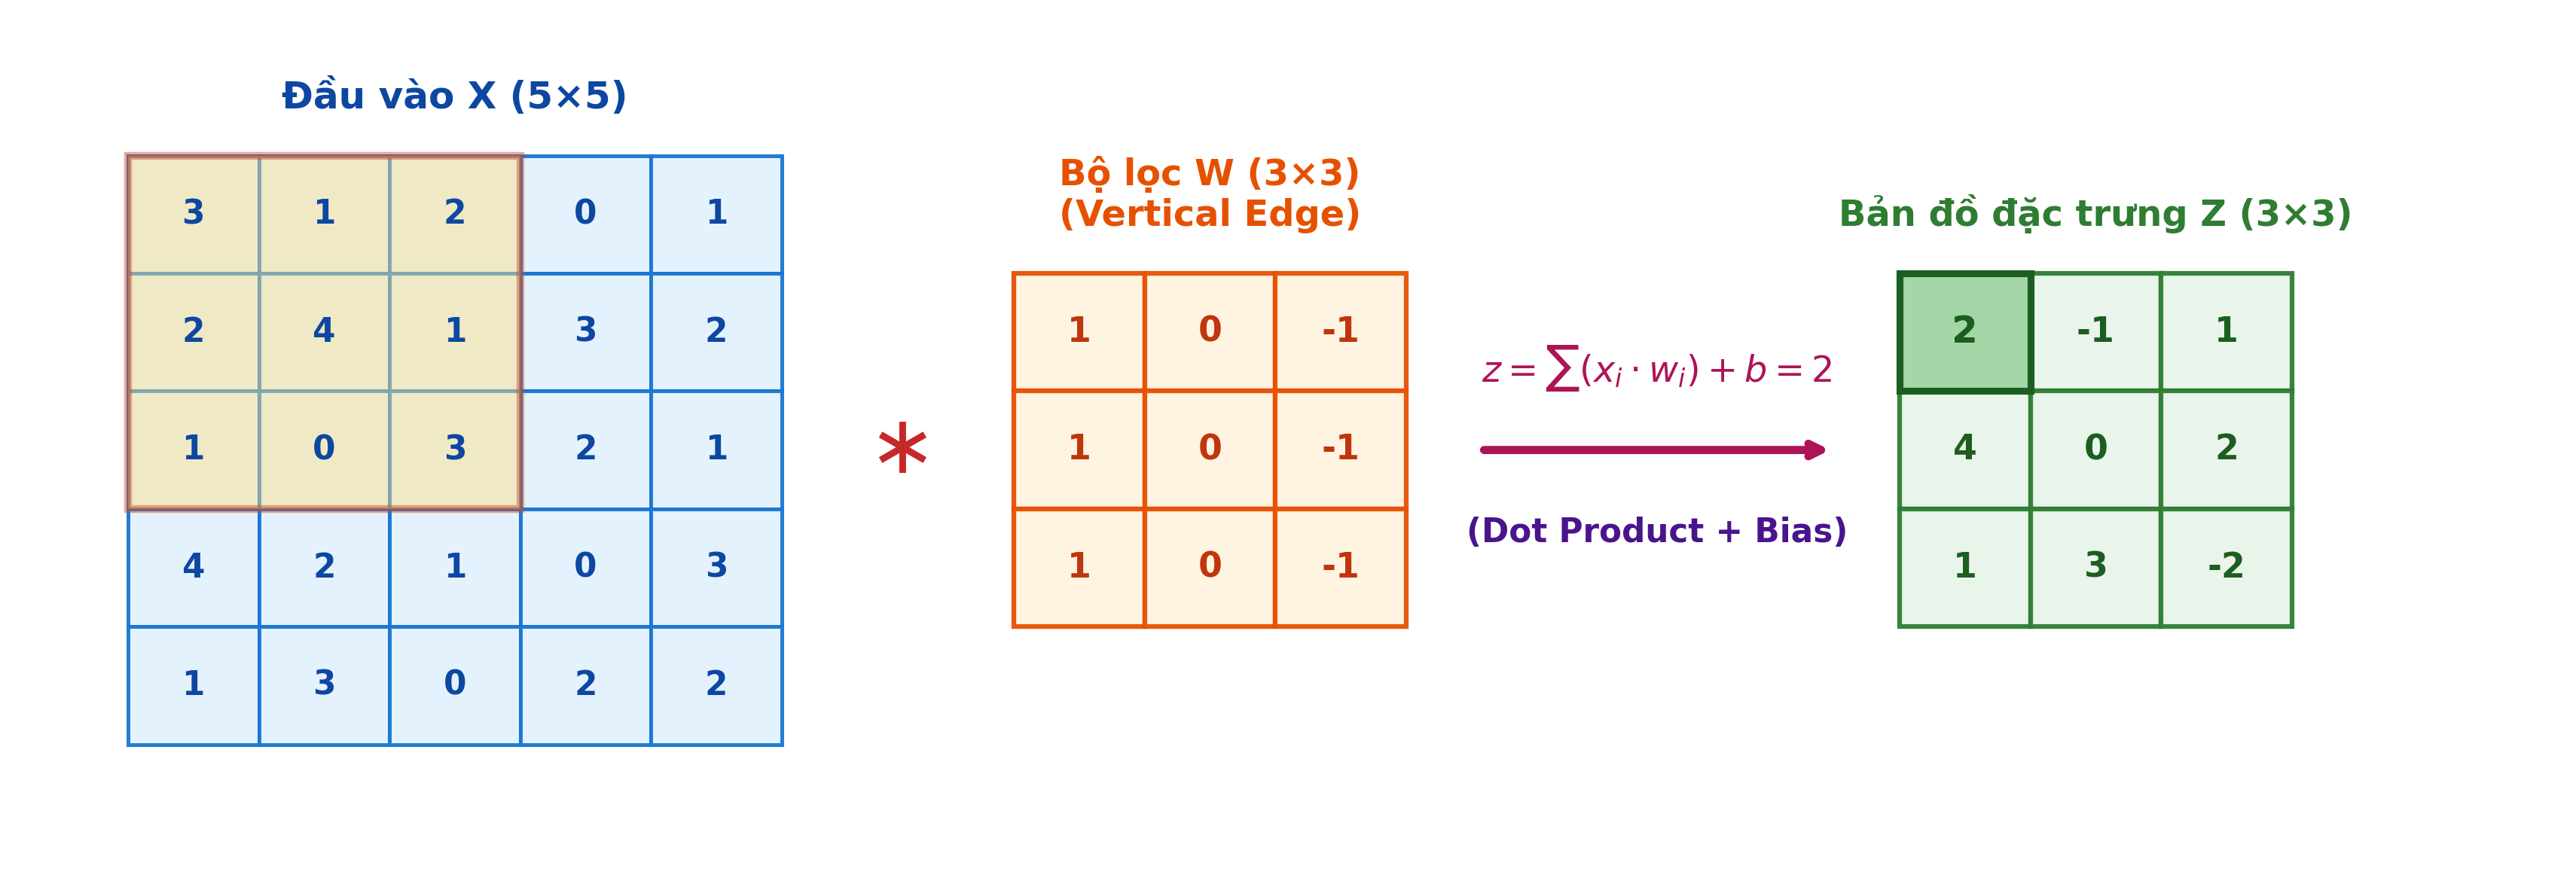
\includegraphics[width=0.92\textwidth]{images/theory_convolution_operation.png}
\caption{Trực quan hóa bản chất tính toán của phép tích chập 2D: Tích vô hướng từng phần tử giữa cửa sổ tiếp nhận cục bộ và bộ lọc trọng số}
\label{fig:theory_convolution_operation}
\end{figure}

\section{Các Siêu Tham Số Hình Học: Đệm Viền, Bước Trượt \& Tích Chập Giãn Nở}
Kích thước và độ chi tiết của bản đồ đặc trưng đầu ra được chi phối trực tiếp bởi ba siêu tham số hình học:

\subsection{Đệm viền (Zero-Padding -- $P$)}
Kỹ thuật đệm thêm các giá trị 0 bao quanh viền của ảnh đầu vào:
\begin{itemize}
    \item \textbf{Valid Padding ($P = 0$):} Không đệm viền. Kích thước bản đồ đặc trưng bị co cụm sau mỗi tầng, đồng thời các điểm ảnh ở rìa ảnh ít được tham gia tính toán dẫn đến mất thông tin biên.
    \item \textbf{Same Padding ($P = 1$ với bộ lọc $3 \times 3$):} Đệm đối xứng giúp bảo toàn nguyên vẹn kích thước không gian ($H_{\text{out}} = H_{\text{in}}$), là điều kiện bắt buộc để có thể xếp chồng hàng chục tầng nơ-ron sâu (như VGG, ResNet).
\end{itemize}

\begin{figure}[H]
\centering
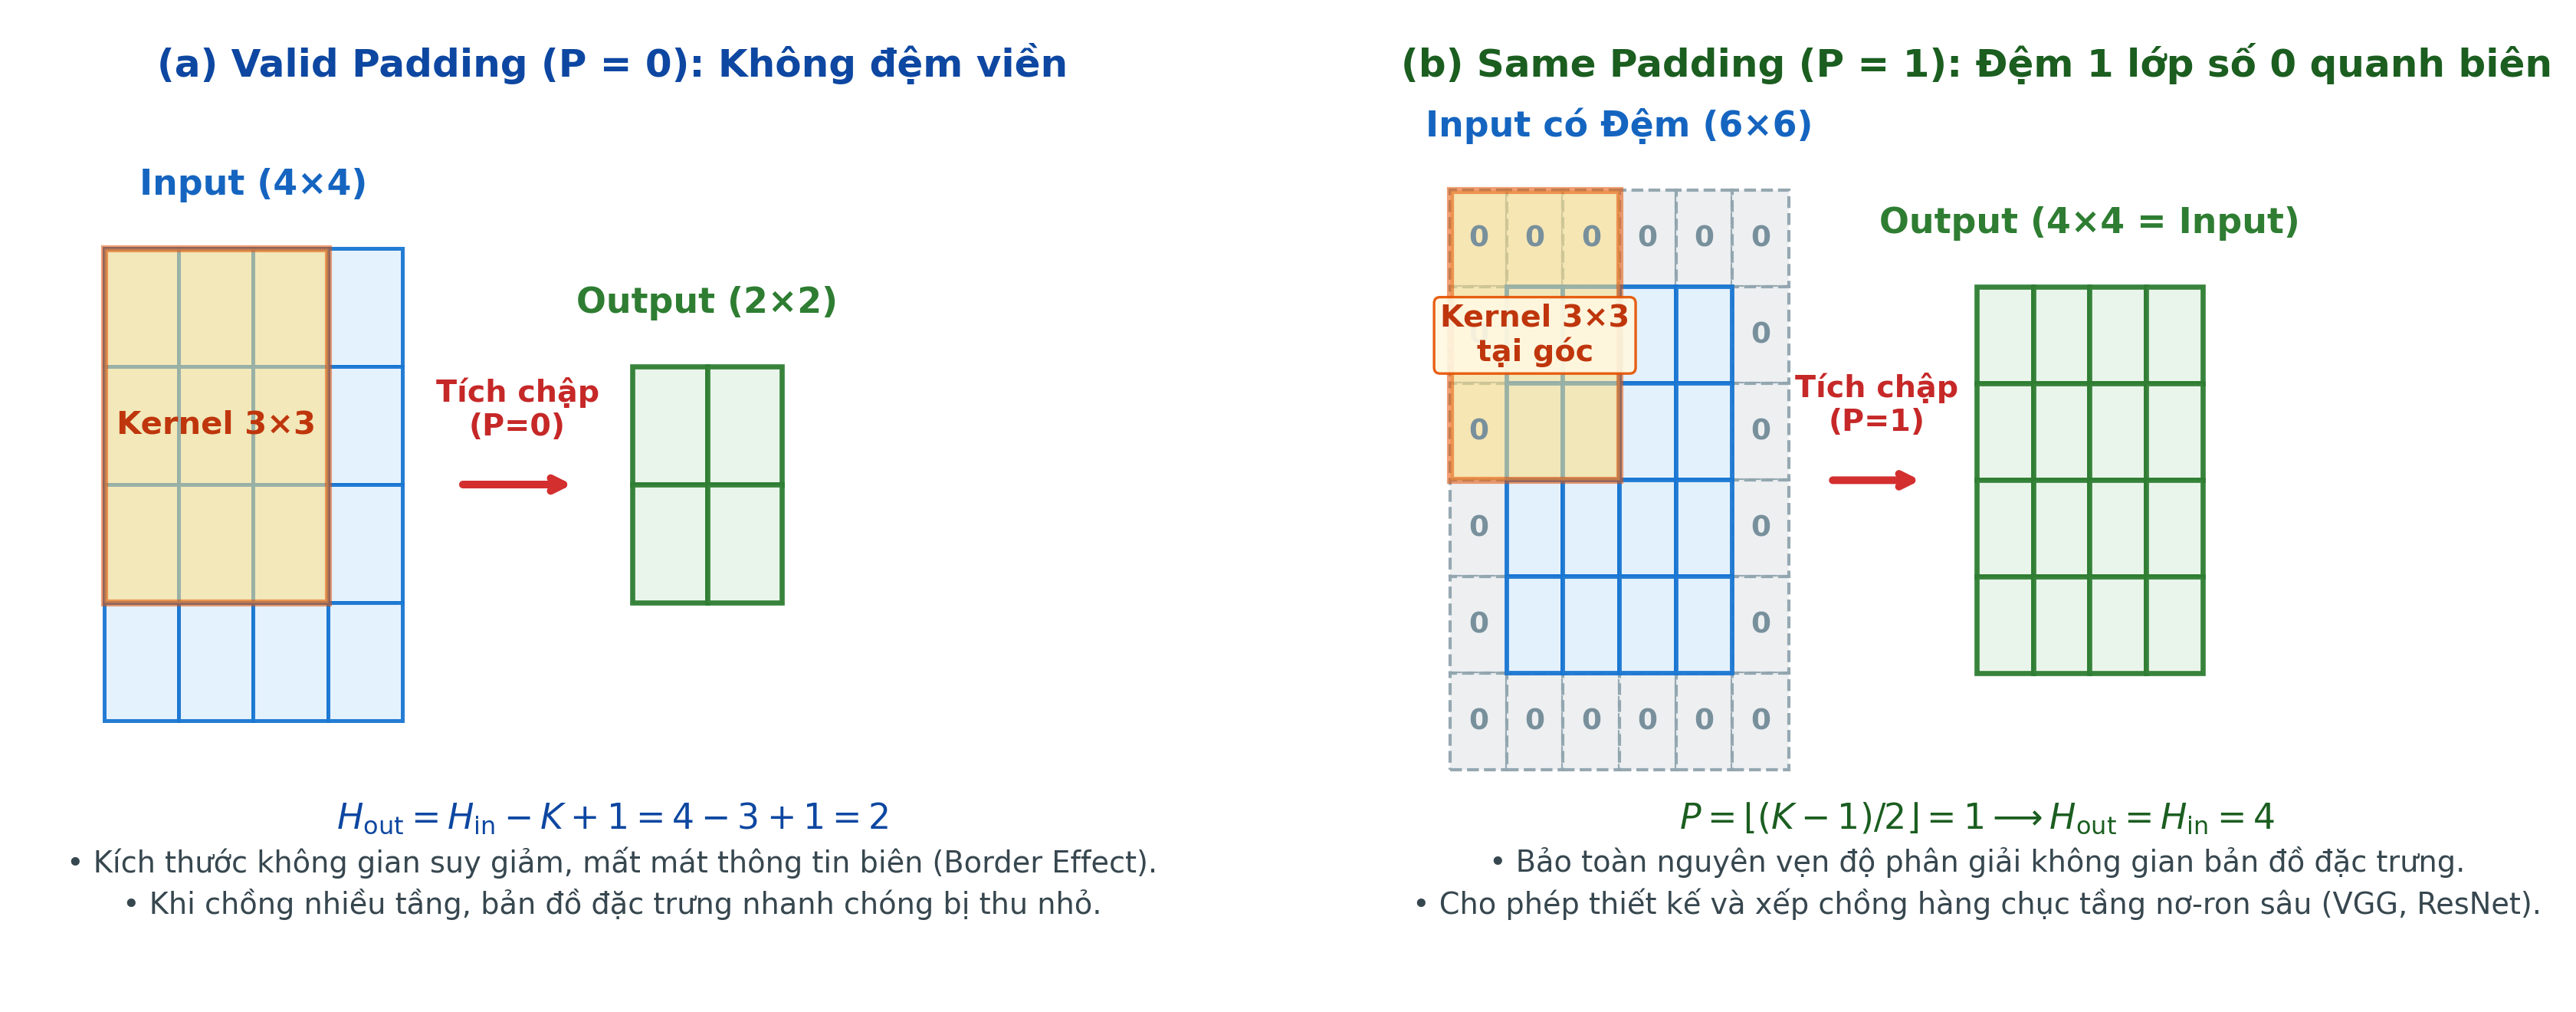
\includegraphics[width=0.90\textwidth]{images/theory_zero_padding.png}
\caption{Trực quan hóa kỹ thuật đệm viền Zero-Padding: (a) Valid Padding ($P=0$) làm suy giảm độ phân giải không gian; (b) Same Padding ($P=1$) đệm số 0 quanh biên giúp bảo toàn nguyên vẹn kích thước không gian $H_{\text{out}} = H_{\text{in}}$}
\label{fig:theory_zero_padding}
\end{figure}

\subsection{Bước trượt (Stride -- $s$)}
Khoảng cách dịch chuyển của bộ lọc sau mỗi lần tính toán:
\begin{itemize}
    \item Khi $s = 1$, bộ lọc dịch chuyển từng điểm ảnh kế tiếp, thu được bản đồ đặc trưng có độ mịn tối đa.
    \item Khi $s = 2$, bộ lọc nhảy cách 2 điểm ảnh, thực hiện giảm một nửa độ phân giải không gian (Downsampling), tương đương chức năng của tầng gộp nhưng có khả năng học được tham số nén.
\end{itemize}

\begin{figure}[H]
\centering
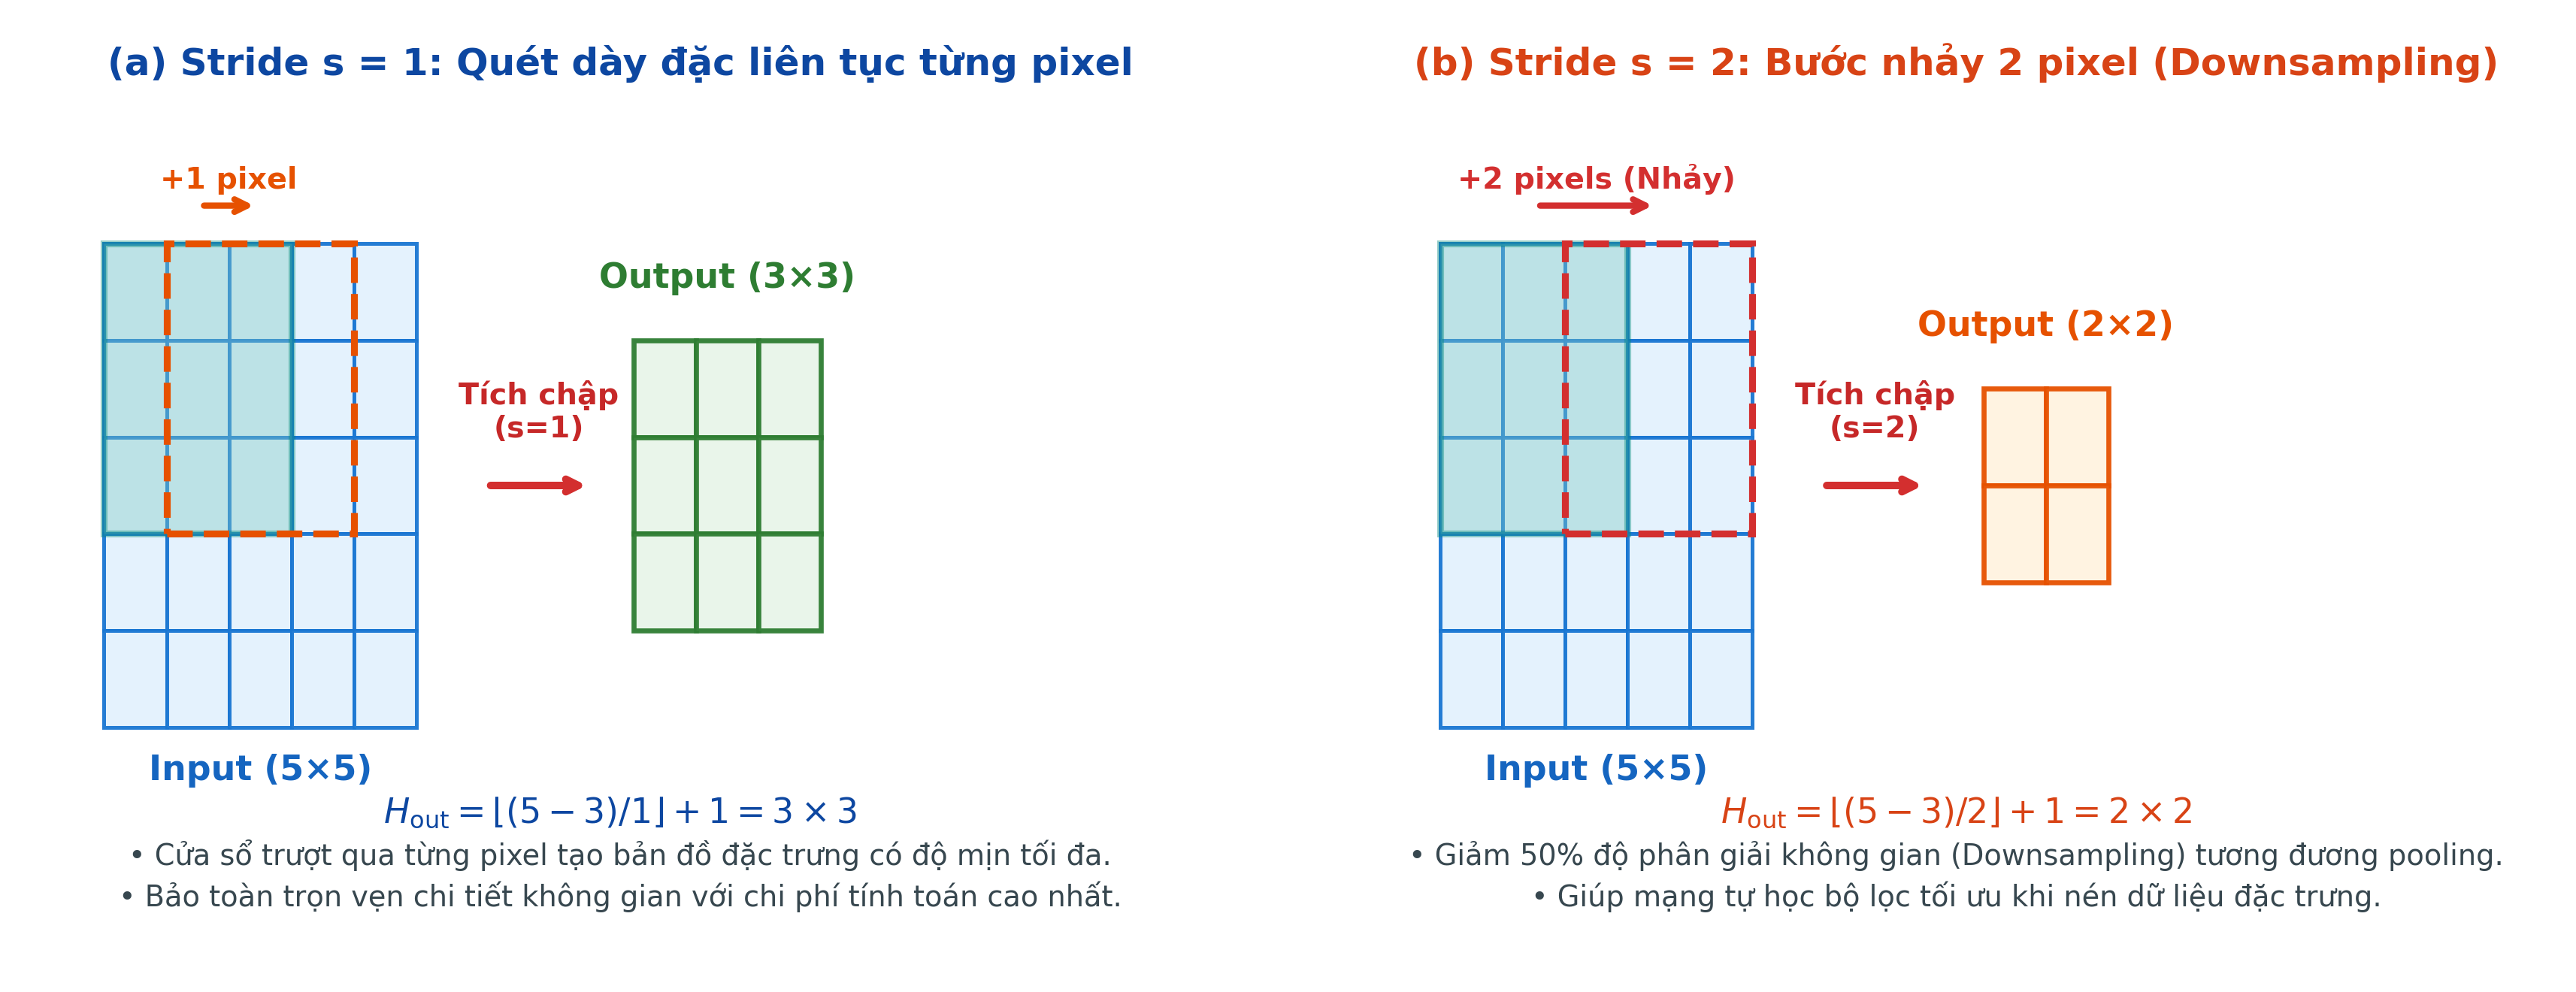
\includegraphics[width=0.90\textwidth]{images/theory_stride.png}
\caption{Trực quan hóa cơ chế bước trượt Stride: (a) Stride $s=1$ quét liên tục từng pixel; (b) Stride $s=2$ nhảy bước 2 pixel thực hiện giảm độ phân giải không gian (Downsampling)}
\label{fig:theory_stride}
\end{figure}

\subsection{Độ giãn nở (Dilation Rate -- $d$)}
Chèn thêm các khoảng trống vào giữa các phần tử của bộ lọc:
\begin{itemize}
    \item Bộ lọc chuẩn $3 \times 3$ tương ứng với độ giãn nở $d = 1$.
    \item Khi cấu hình $d = 2$, khoảng cách giữa các phần tử trọng số tăng lên, mở rộng phạm vi bao phủ tương đương vùng $5 \times 5$ trên ảnh gốc nhưng vẫn giữ nguyên đúng 9 trọng số cần học, không làm tăng tham số hay chi phí lưu trữ.
\end{itemize}

\begin{figure}[H]
\centering
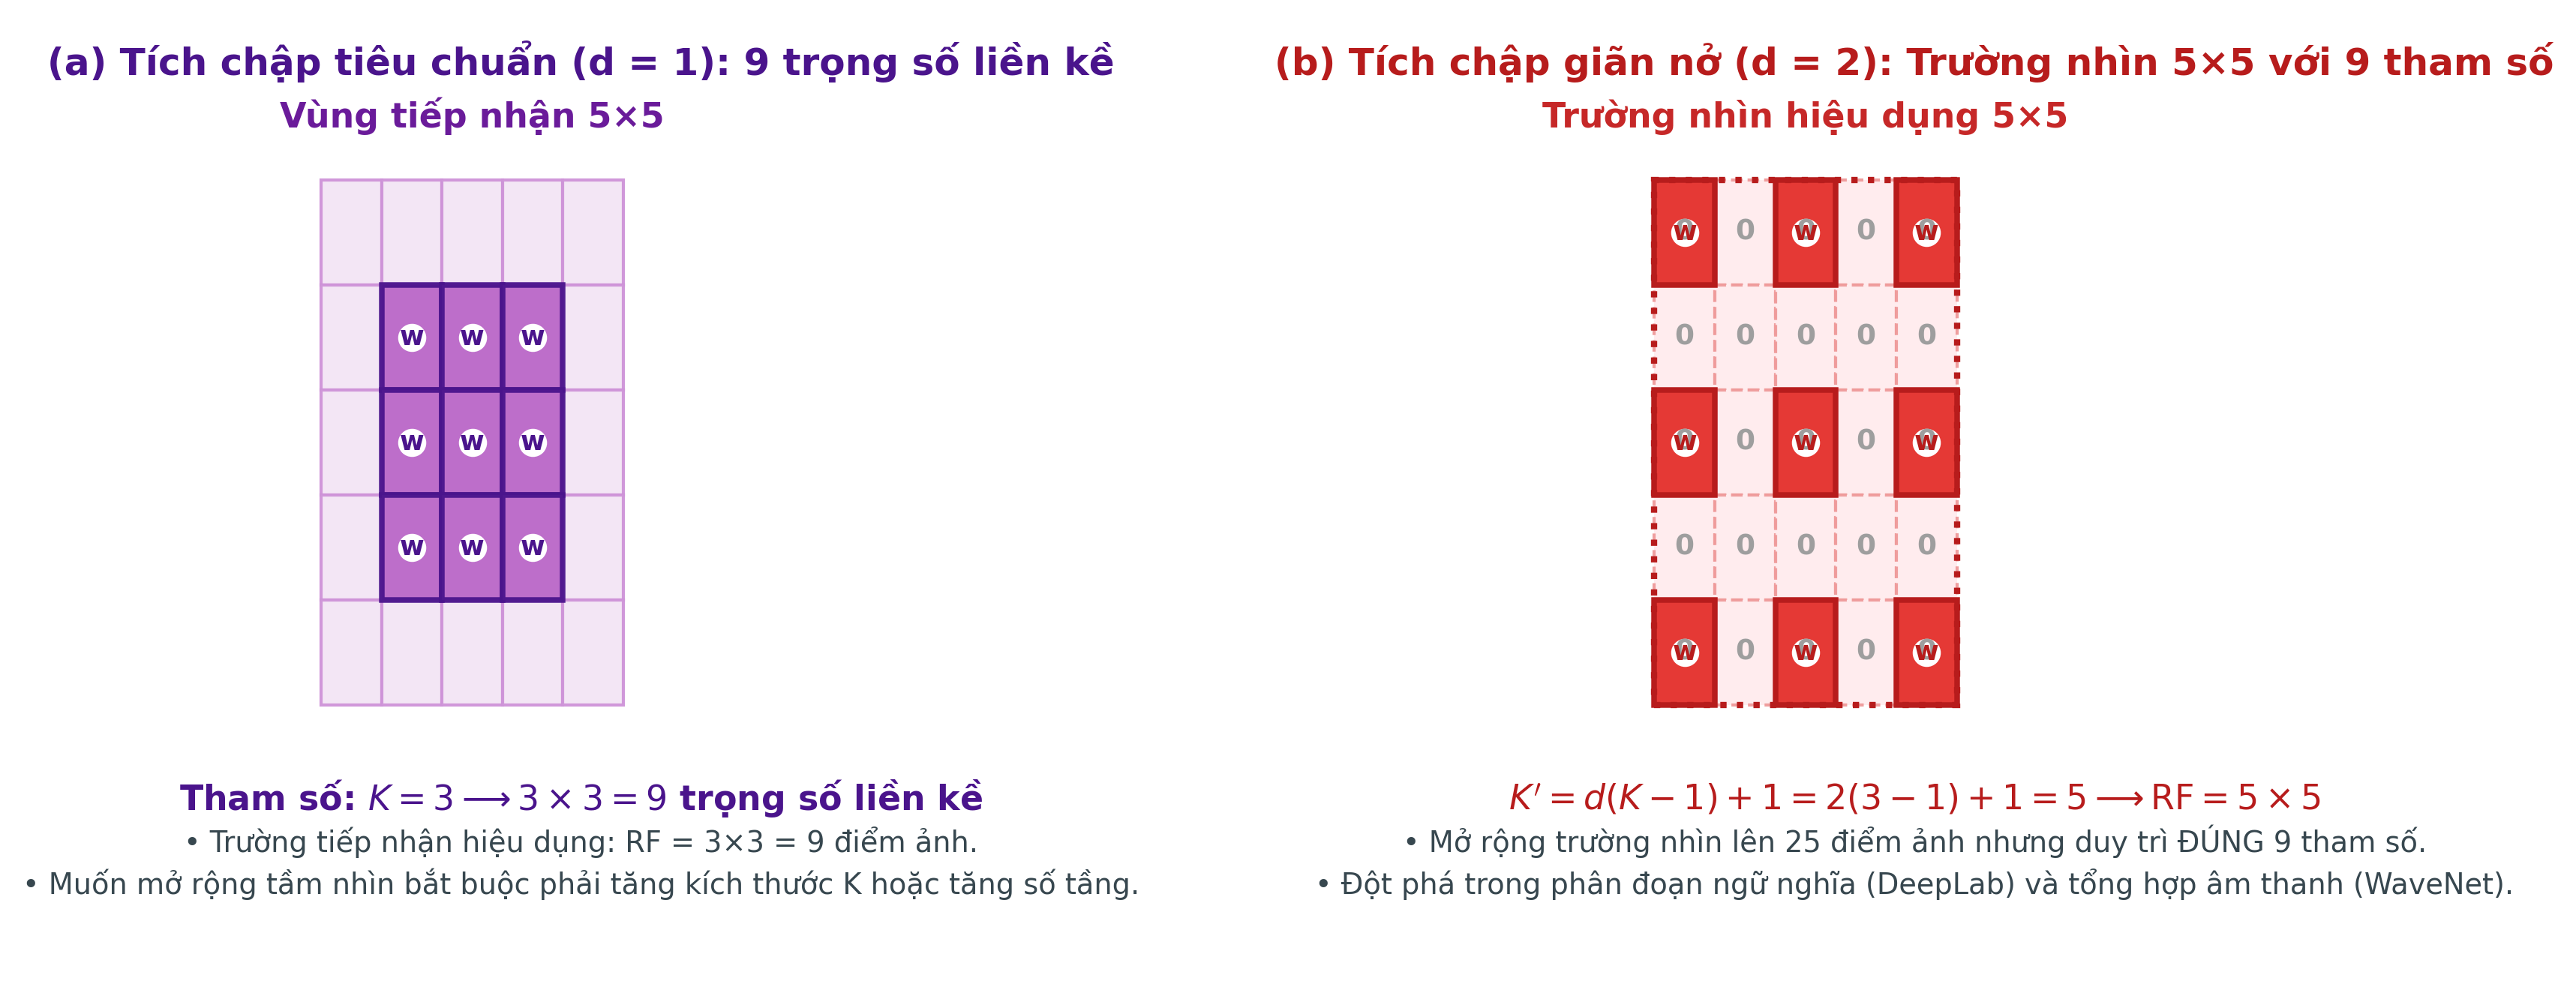
\includegraphics[width=0.90\textwidth]{images/theory_dilation.png}
\caption{Trực quan hóa tích chập giãn nở Dilated Convolution: (a) Bộ lọc chuẩn $3 \times 3$ ($d=1$); (b) Bộ lọc giãn nở $d=2$ mở rộng trường tiếp nhận tương đương vùng $5 \times 5$ với đúng 9 tham số trọng số}
\label{fig:theory_dilation}
\end{figure}

\subsection{Công thức tính kích thước bản đồ đặc trưng đầu ra}
Kích thước không gian $(H_{\text{out}}, W_{\text{out}})$ của bản đồ đặc trưng được xác định theo công thức:
\begin{equation}
    H_{\text{out}} = \left\lfloor \frac{H_{\text{in}} + 2P - d(K - 1) - 1}{s} \right\rfloor + 1, \quad W_{\text{out}} = \left\lfloor \frac{W_{\text{in}} + 2P - d(K - 1) - 1}{s} \right\rfloor + 1
\end{equation}
Trong cấu hình tích chập thông thường ($d = 1$), công thức rút gọn thành:
\begin{equation}
    H_{\text{out}} = \left\lfloor \frac{H_{\text{in}} + 2P - K}{s} \right\rfloor + 1
\end{equation}

\section{Trường Tiếp Nhận Cục Bộ (Receptive Field) \& Lợi Thế Của Bộ Lọc Nhỏ}
\subsection{Khái niệm trường tiếp nhận cục bộ (Receptive Field -- RF)}
Trường tiếp nhận là kích thước vùng không gian trên ảnh đầu vào gốc mà một nơ-ron ở tầng sau có thể "nhìn thấy" và chịu sự chi phối. 
\begin{itemize}
    \item Tại tầng tích chập đầu tiên với bộ lọc $3 \times 3$, mỗi nơ-ron quan sát trực tiếp vùng $3 \times 3$ trên ảnh gốc ($RF = 3$).
    \item Khi đi qua tầng tích chập $3 \times 3$ tiếp theo, mỗi nơ-ron tầng hai tổng hợp thông tin từ vùng $3 \times 3$ của tầng một, qua đó gián tiếp bao phủ một vùng không gian có kích thước $5 \times 5$ trên ảnh gốc ($RF = 5$).
\end{itemize}

\subsection{Ưu thế khi xếp chồng nhiều bộ lọc nhỏ $3 \times 3$}
Thay vì sử dụng một bộ lọc kích thước lớn $5 \times 5$, các kiến trúc hiện đại (như VGG, ResNet) đều ưu tiên xếp chồng hai tầng tích chập nhỏ $3 \times 3$:
\begin{itemize}
    \item \textbf{Tiết kiệm 28\% số lượng tham số:} 
    Một tầng $5 \times 5$ với $C$ kênh cần $5 \times 5 \times C^2 = 25C^2$ tham số. Trong khi đó, hai tầng $3 \times 3$ liên tiếp chỉ tiêu tốn $(3 \times 3 + 3 \times 3)C^2 = 18C^2$ tham số, giảm gần một phần ba chi phí lưu trữ.
    \item \textbf{Tăng cường khả năng biểu diễn phi tuyến:} 
    Việc sử dụng hai tầng cho phép chèn thêm một hàm kích hoạt phi tuyến (ReLU) ở giữa, giúp mạng học được các hàm phân tách phức tạp và giàu ngữ nghĩa hơn.
\end{itemize}

\begin{figure}[H]
\centering
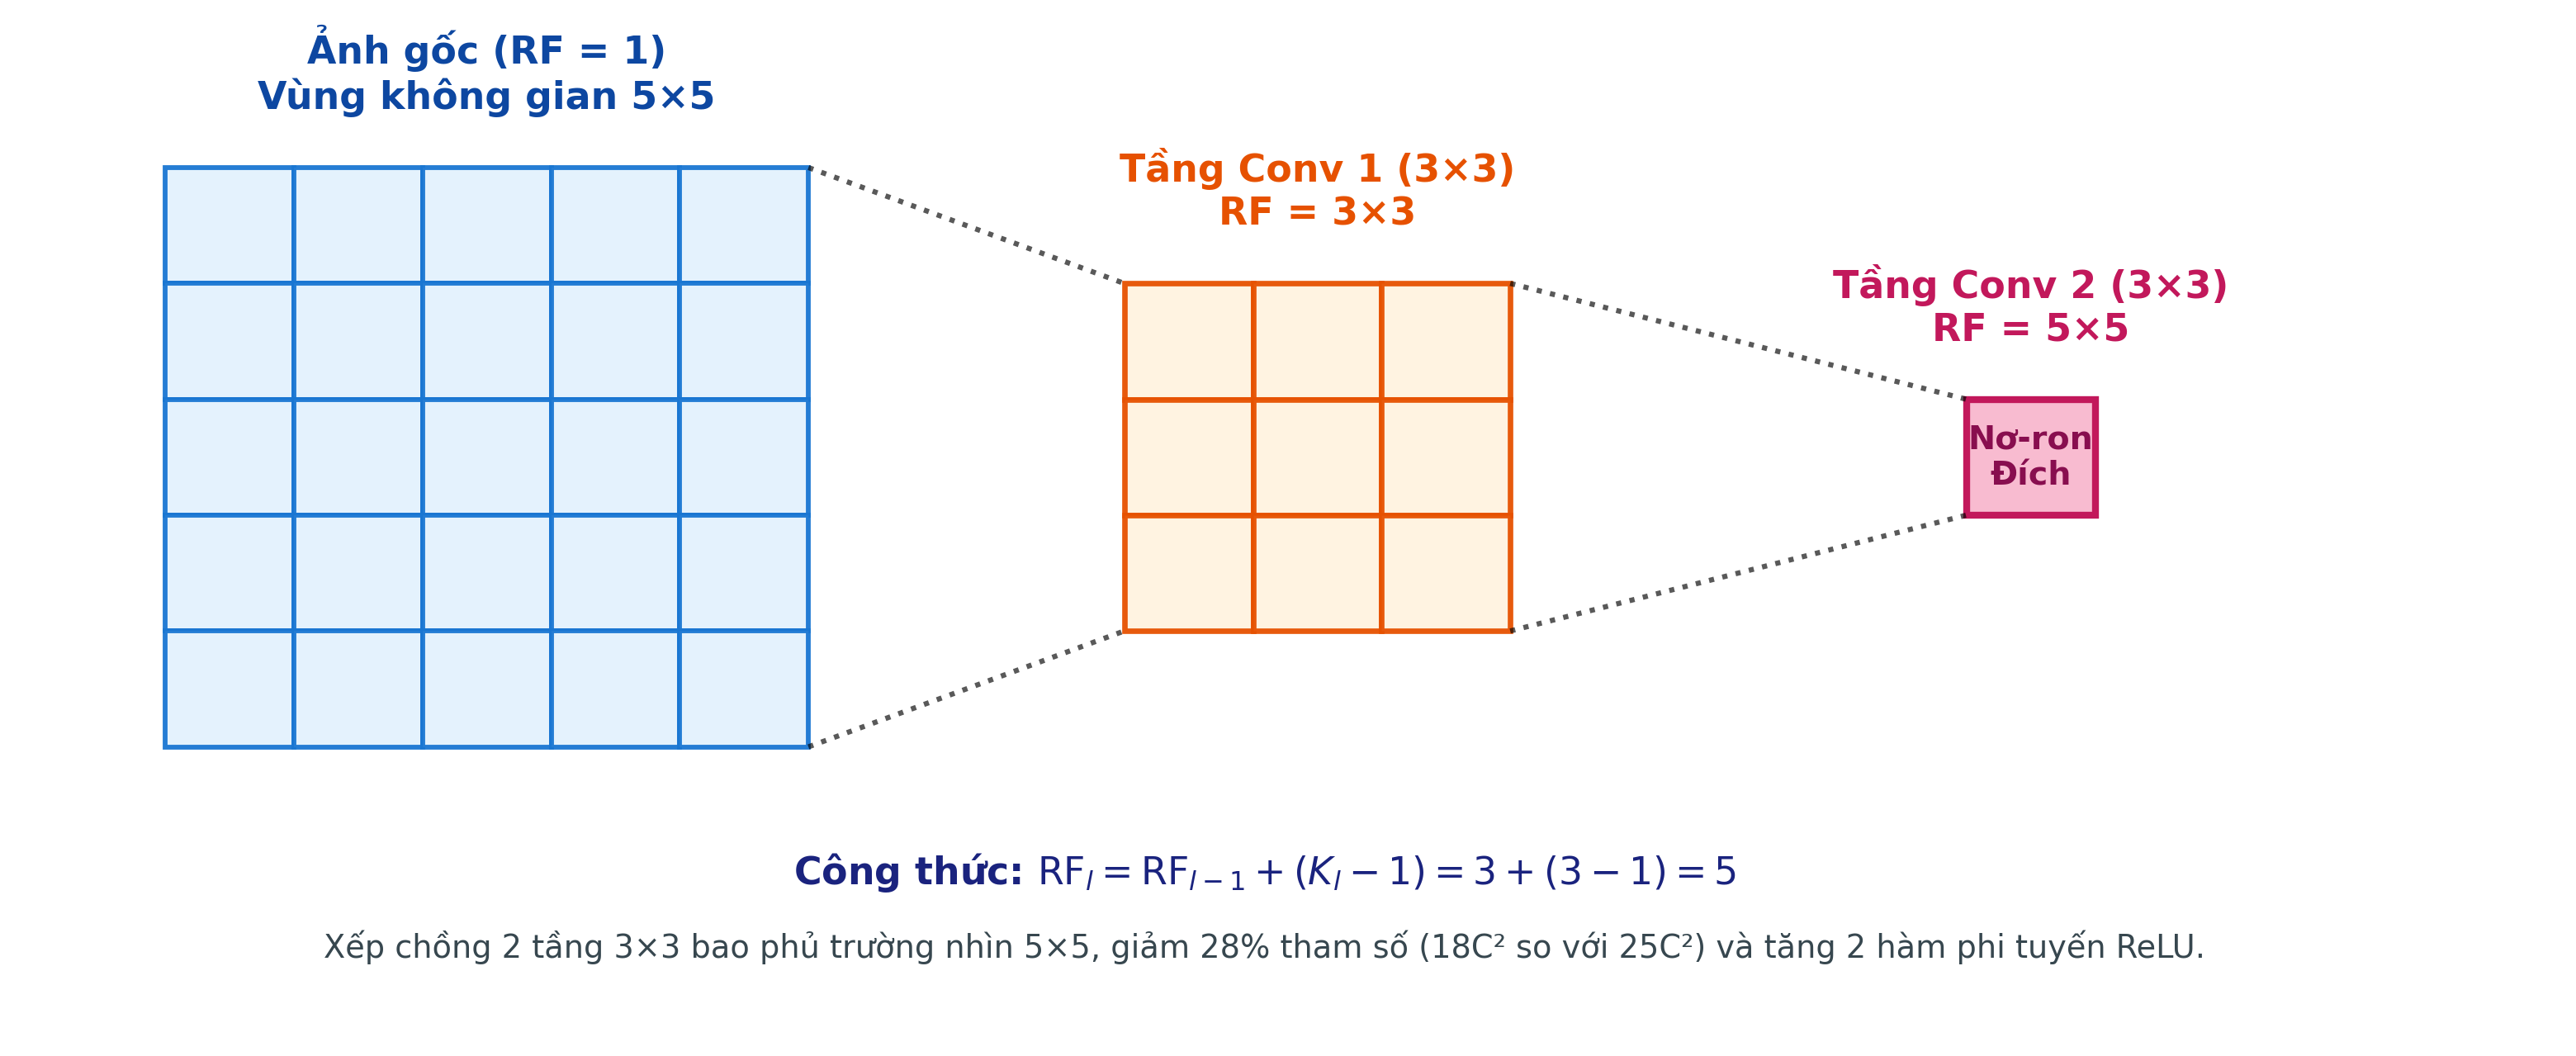
\includegraphics[width=0.78\textwidth]{images/theory_receptive_field.png}
\caption{Sự mở rộng trường tiếp nhận hiệu dụng (Receptive Field): Hai tầng tích chập $3 \times 3$ liên tiếp bao phủ vùng không gian $5 \times 5$ trên ảnh gốc với số tham số ít hơn 28\%}
\label{fig:theory_receptive_field}
\end{figure}

\subsection{Tính tương đương tịnh tiến và bất biến tịnh tiến}
Hai đặc tính nền tảng bảo đảm sự ổn định của mạng tích chập:
\begin{itemize}
    \item \textbf{Tính tương đương tịnh tiến (Translation Equivariance -- ở tầng Conv):} Khi đối tượng trong ảnh dịch chuyển vị trí, bản đồ đặc trưng thu được cũng dịch chuyển một khoảng tương ứng mà không bị mất dấu.
    \item \textbf{Tính bất biến tịnh tiến (Translation Invariance -- ở tầng Pooling):} Khi đối tượng trong ảnh xê dịch nhẹ trong phạm vi lân cận, giá trị đầu ra sau tầng gộp vẫn giữ nguyên, giúp mạng nhận diện đối tượng ổn định trước các biến dạng vị trí nhỏ.
\end{itemize}

\section{Tầng Gộp (Pooling) \& Cơ Chế Lan Truyền Ngược Gradient}
Sau khi trích xuất đặc trưng qua tầng tích chập và hàm kích hoạt phi tuyến, tầng gộp (Pooling) thực hiện nén kích thước không gian nhằm giảm chi phí tính toán và hạn chế quá khớp.

\subsection{Các cơ chế gộp đặc trưng phổ biến}
\begin{enumerate}
    \item \textbf{Max Pooling:} Lấy giá trị kích hoạt lớn nhất trong cửa sổ gộp (ví dụ $2 \times 2$). Phương pháp này giữ lại đặc trưng phản hồi mạnh nhất, loại bỏ nhiễu nền và giảm một nửa kích thước không gian.
    \item \textbf{Average Pooling:} Tính trung bình cộng các giá trị trong cửa sổ, giúp làm mịn tín hiệu.
    \item \textbf{Global Average Pooling (GAP):} Tính trung bình trên toàn bộ chiều cao và chiều rộng của bản đồ đặc trưng, nén mỗi kênh kích thước $H \times W$ thành một giá trị vô hướng duy nhất. GAP thay thế hoàn toàn tầng Flatten truyền thống, giảm 80--90\% tham số ở các tầng cuối của mạng và chống quá khớp triệt để.
\end{enumerate}

\begin{figure}[H]
\centering
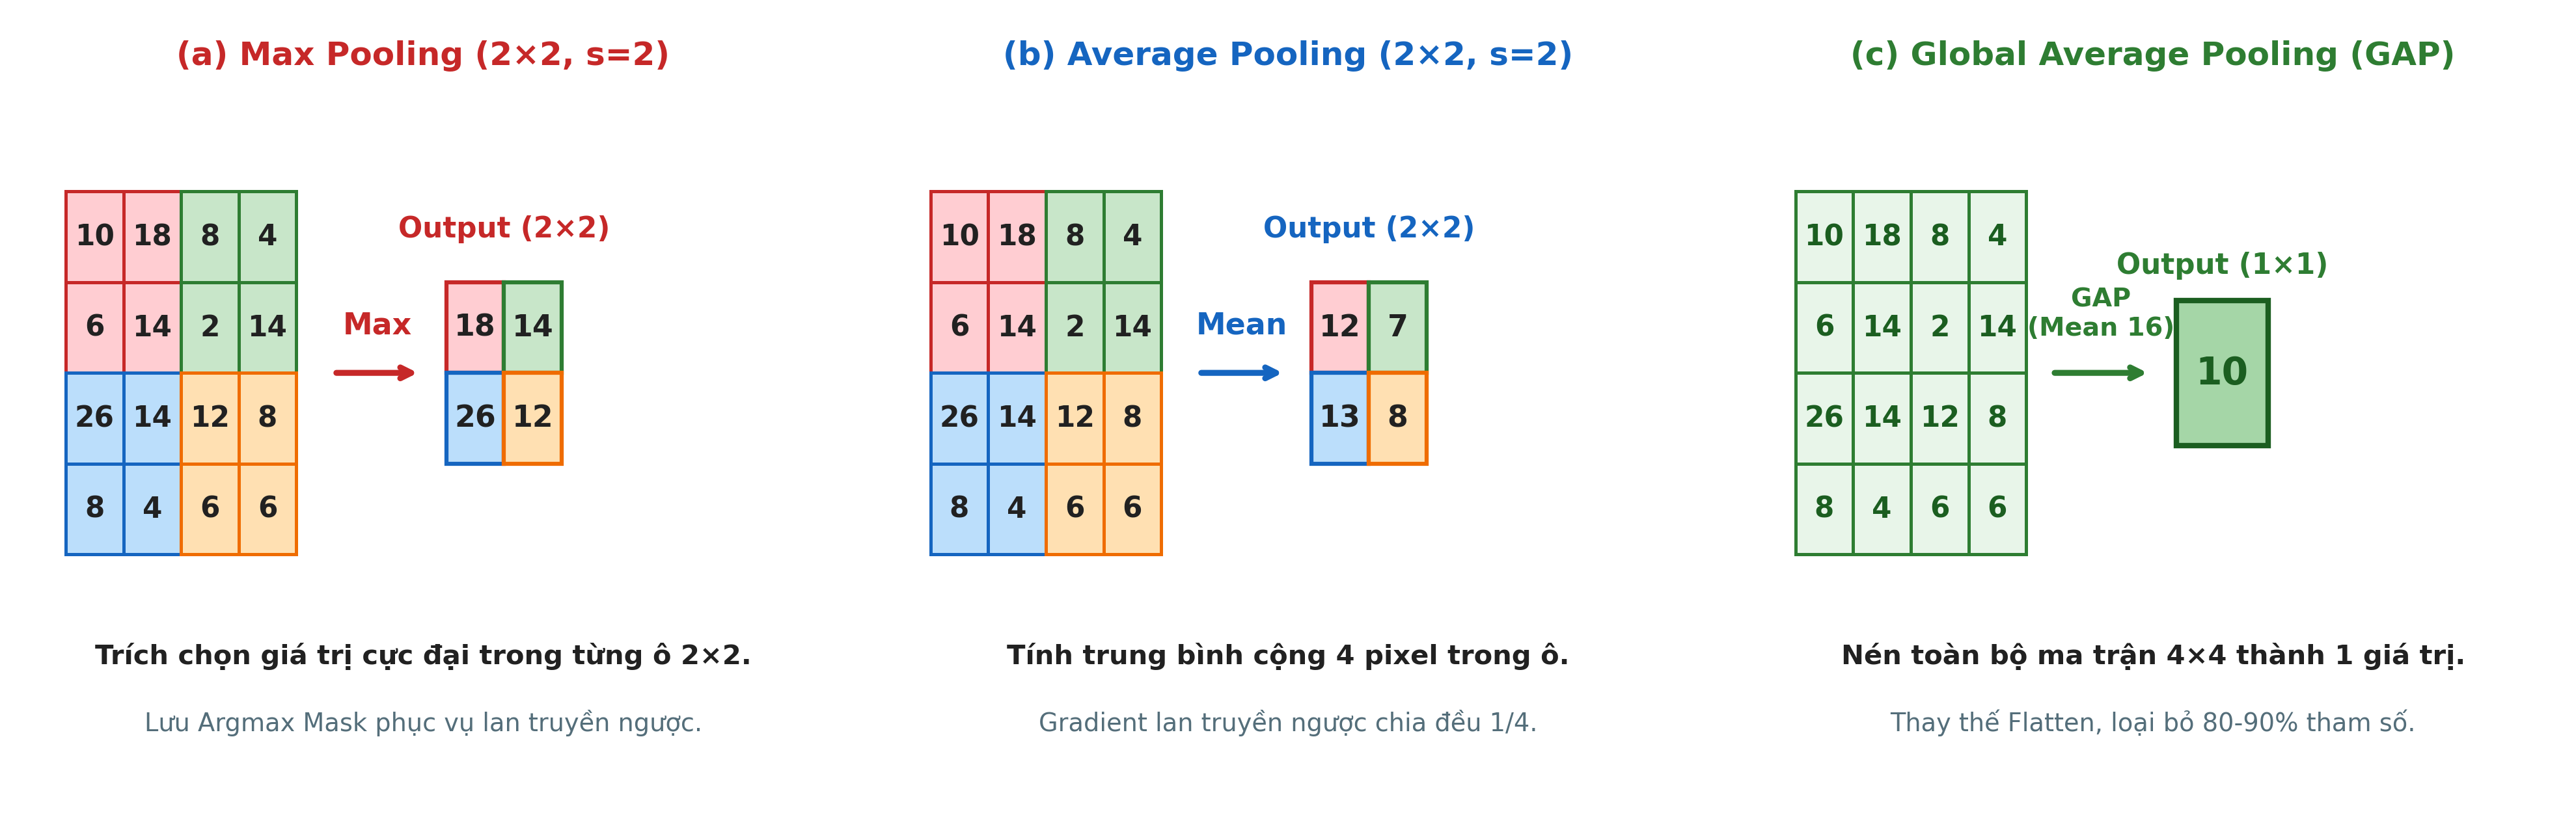
\includegraphics[width=0.95\textwidth]{images/theory_pooling_mechanisms.png}
\caption{Trực quan hóa các cơ chế tầng gộp đặc trưng: (a) Max Pooling trích chọn giá trị cực đại; (b) Average Pooling tính giá trị trung bình; (c) Global Average Pooling (GAP) nén toàn bộ bản đồ đặc trưng thành một giá trị vô hướng duy nhất}
\label{fig:theory_pooling_mechanisms}
\end{figure}

\subsection{Cơ chế lan truyền ngược gradient qua tầng Pooling}
\begin{itemize}
    \item \textbf{Max Pooling:} Trong pha lan truyền tiến, mạng ghi nhớ vị trí (chỉ số) của nơ-ron đạt giá trị cực đại qua mặt nạ \textit{argmax}. Trong pha lan truyền ngược, gradient từ tầng sau chỉ được truyền toàn vẹn về đúng nơ-ron chiến thắng đó; các vị trí còn lại nhận gradient bằng 0.
    \item \textbf{Average Pooling:} Do tất cả các phần tử trong cửa sổ đều đóng góp như nhau vào giá trị trung bình, gradient từ tầng sau được chia đều cho toàn bộ các phần tử trong cửa sổ gộp.
\end{itemize}

\section{Tối Ưu Hóa Tính Toán: Thuật Toán im2col \& Khởi Tạo Trọng Số He Normal}
\subsection{Kỹ thuật vector hóa với thuật toán im2col và GEMM}
Nếu thực thi phép tích chập bằng các vòng lặp lồng nhau lặp qua từng pixel, tốc độ thực thi trong Python sẽ rất chậm. Để tối ưu hóa hiệu năng trên thư viện NumPy thuần, thuật toán \textbf{im2col} (Image-to-Column) được áp dụng:
\begin{itemize}
    \item Thuật toán trải phẳng từng cửa sổ trượt cục bộ thành một hàng của ma trận dữ liệu $\mathbf{X}_{\text{col}}$.
    \item Dàn phẳng ma trận trọng số $\mathbf{W}$ thành $\mathbf{W}_{\text{row}}$.
    \item Toàn bộ phép tích chập trên mini-batch được quy về một phép nhân ma trận tổng quát (\textbf{GEMM} -- General Matrix Multiply) duy nhất:
    \begin{equation}
        \mathbf{Z}_{\text{col}} = \mathbf{X}_{\text{col}} \mathbf{W}_{\text{row}} + \mathbf{b}
    \end{equation}
\end{itemize}

\begin{figure}[H]
\centering
\resizebox{0.92\textwidth}{!}{
\begin{tikzpicture}[node distance=1.8cm, auto]
    \node [draw, rectangle, fill=blue!12, rounded corners, minimum height=1.1cm, text centered] (input) {Tensor Đầu Vào: $(N, C_{\text{in}}, H, W)$};
    \node [draw, rectangle, fill=orange!18, rounded corners, right=1.2cm of input, minimum height=1.1cm, text centered] (im2col) {im2col: $\mathbf{X}_{\text{col}} \in \mathbb{R}^{(N H_{\text{out}} W_{\text{out}}) \times (C_{\text{in}} K_H K_W)}$};
    \node [draw, rectangle, fill=green!18, rounded corners, right=1.2cm of im2col, minimum height=1.1cm, text centered] (gemm) {GEMM: $\mathbf{Z}_{\text{col}} = \mathbf{X}_{\text{col}} \mathbf{W}_{\text{row}} + \mathbf{b}$};
    \draw [->, thick, >=stealth] (input) -- (im2col);
    \draw [->, thick, >=stealth] (im2col) -- (gemm);
\end{tikzpicture}
}
\caption{Quy trình vector hóa phép tích chập bằng thuật toán im2col và phép nhân ma trận GEMM}
\label{fig:im2col_flow}
\end{figure}

\subsection{Lan truyền ngược gradient qua đại số ma trận}
Nhờ cấu trúc ma trận của \texttt{im2col}, pha lan truyền ngược được tính toán đơn giản và tức thì thông qua phép nhân ma trận chuyển vị:
\begin{equation}
    \frac{\partial \mathcal{L}}{\partial \mathbf{W}_{\text{row}}} = \mathbf{X}_{\text{col}}^T \frac{\partial \mathcal{L}}{\partial \mathbf{Z}_{\text{col}}}, \quad \frac{\partial \mathcal{L}}{\partial \mathbf{X}_{\text{col}}} = \frac{\partial \mathcal{L}}{\partial \mathbf{Z}_{\text{col}}} \mathbf{W}_{\text{row}}^T
\end{equation}
Sau đó, hàm \texttt{col2im} đảo ngược thao tác, cộng dồn các giá trị gradient tại các vùng trượt chồng lấn để hoàn nguyên tensor gradient $\frac{\partial \mathcal{L}}{\partial \mathbf{X}}$ ban đầu cho các tầng trước.

\subsection{Nguyên lý khởi tạo trọng số He Normal (Kaiming Normal)}
Trong các mạng sâu sử dụng hàm kích hoạt phi tuyến ReLU ($a = \max(0, z)$), vì một nửa tín hiệu (vùng giá trị âm) bị gán bằng 0, phương sai của tín hiệu kích hoạt sẽ bị suy giảm một nửa sau mỗi tầng. Nếu áp dụng cách khởi tạo thông thường, tín hiệu truyền qua nhiều tầng sẽ nhanh chóng tắt dần về 0 (triệt tiêu gradient).

Để khắc phục hiện tượng này, phương pháp He Normal (Kaiming He et al., 2015) tăng gấp đôi phương sai khởi tạo của ma trận trọng số:
\begin{equation}
    \text{Var}(\mathbf{W}) = \frac{2}{n_{\text{in}}} = \frac{2}{C_{\text{in}} \cdot K_H \cdot K_W}
\end{equation}
Trọng số bộ lọc được khởi tạo theo phân phối chuẩn Gauss:
\begin{equation}
    \mathbf{W} \sim \mathcal{N}\left(0, \; \sigma^2 = \frac{2}{C_{\text{in}} \cdot K_H \cdot K_W}\right)
\end{equation}
nhờ đó bảo toàn độ phân tán của tín hiệu và giữ cho dòng chảy gradient ổn định qua toàn bộ mạng.

\section{Hệ Thống Hóa Các Khái Niệm Nền Tảng Cốt Lõi Trong CNN}
Nhằm hệ thống hóa toàn diện nền tảng lý thuyết trước khi bước vào các bài toán thực nghiệm chuyên sâu, phần này tổng hợp 16 câu hỏi -- đáp cốt lõi định hình nguyên lý vận hành của mạng nơ-ron tích chập (CNN):

\begin{enumerate}[label=\textbf{\arabic*.}]
    \item \textbf{Sự khác biệt bản chất giữa tầng Dense và tầng Conv là gì?}
    Tầng Dense liên kết toàn bộ mọi đặc trưng đầu vào với từng nơ-ron, phá hủy cấu trúc không gian và làm bùng nổ tham số. Tầng Conv chỉ liên kết cục bộ trong cửa sổ trượt nhỏ và dùng chung một bộ trọng số (Weight Sharing) trên toàn bộ không gian ảnh.
    
    \item \textbf{Ý nghĩa của phương trình hợp hàm tổng quát $\hat{y} = (f_L \circ \dots \circ f_1)(\mathbf{X})$ trong CNN?}
    Mạng CNN là sự xếp chồng tuần tự của các hàm biến đổi tham số hóa: các tầng đầu trích xuất đặc trưng sơ cấp (cạnh, góc, viền); các tầng giữa kết hợp thành họa tiết, bộ phận; và các tầng cuối ánh xạ thành biểu diễn ngữ nghĩa trừu tượng để đưa ra dự đoán.
    
    \item \textbf{Cơ chế nào giúp CNN giải quyết triệt để vấn đề bùng nổ tham số?}
    Nhờ nguyên lý chia sẻ trọng số (Weight Sharing), số lượng tham số của tầng Conv chỉ phụ thuộc vào kích thước bộ lọc $(K_H \times K_W \times C_{\text{in}} \times C_{\text{out}})$ mà hoàn toàn độc lập với kích thước không gian ảnh đầu vào $(H \times W)$.
    
    \item \textbf{Phân biệt phép tích chập (Convolution) và tương quan chéo (Cross-Correlation):}
    Tích chập giải tích lật ngược bộ lọc trước khi nhân chập để đảm bảo tính giao hoán. Tương quan chéo trượt thẳng bộ lọc mà không lật. Trong học sâu, vì các trọng số bộ lọc được học tự do từ dữ liệu, thao tác tương quan chéo vẫn cho năng lực biểu diễn tương đương và được quy ước gọi chung là tích chập.
    
    \item \textbf{Trường tiếp nhận (Receptive Field) là gì và vì sao nên dùng nhiều bộ lọc nhỏ $3\times 3$?}
    Trường tiếp nhận là vùng ảnh gốc tác động lên một nơ-ron ở tầng sâu. Hai tầng $3\times 3$ liên tiếp tạo ra trường tiếp nhận $5\times 5$, nhưng tiết kiệm 28\% tham số và bổ sung thêm hàm phi tuyến giúp tăng cường khả năng học biểu diễn.
    
    \item \textbf{Phân biệt tính tương đương tịnh tiến (Equivariance) và tính bất biến tịnh tiến (Invariance)?}
    Tương đương tịnh tiến (ở tầng Conv) nghĩa là khi ảnh dịch chuyển thì bản đồ đặc trưng cũng dịch chuyển tương ứng. Bất biến tịnh tiến (ở tầng Pooling) nghĩa là giá trị đặc trưng được trích xuất không đổi khi ảnh dịch chuyển nhẹ.
    
    \item \textbf{Vai trò của kỹ thuật đệm viền (Zero-Padding)?}
    Ngăn chặn việc kích thước không gian bị thu hẹp quá nhanh qua các tầng sâu, đồng thời bảo tồn trọn vẹn thông tin ở các vùng biên ảnh (tránh Border Effect).
    
    \item \textbf{Bước trượt (Stride) và Tích chập giãn nở (Dilated Convolution) có vai trò gì?}
    Bước trượt $s > 1$ giúp giảm độ phân giải không gian có học. Tích chập giãn nở ($d > 1$) giúp mở rộng trường tiếp nhận theo cấp số nhân mà không làm tăng số lượng tham số hay kích thước ma trận trọng số.
    
    \item \textbf{Cơ chế lan truyền ngược gradient qua tầng Max Pooling diễn ra như thế nào?}
    Gradient chỉ được chuyển toàn bộ về nơ-ron đạt giá trị cực đại trong pha lan truyền tiến (thông qua mặt nạ argmax), các nơ-ron còn lại trong cửa sổ nhận gradient bằng 0.
    
    \item \textbf{Global Average Pooling (GAP) giải quyết vấn đề gì của tầng Flatten?}
    Tầng Flatten kết nối hàng chục nghìn đặc trưng với tầng Dense, chiếm 80--90\% tham số và gây quá khớp nặng. GAP tính trung bình không gian trên từng kênh, giảm tham số triệt để và tăng tính diễn giải trực tiếp cho từng bản đồ đặc trưng.
    
    \item \textbf{Đạo hàm đối với trọng số và đối với đầu vào có bản chất toán học là gì?}
    Đạo hàm đối với trọng số tương đương phép tích chập giữa đầu vào $\mathbf{X}$ và gradient đầu ra $\frac{\partial \mathcal{L}}{\partial \mathbf{Z}}$. Đạo hàm đối với đầu vào tương đương phép tích chập đầy đủ giữa gradient đầu ra và bộ lọc đã xoay 180 độ.
    
    \item \textbf{Thuật toán im2col và col2im tối ưu hóa tính toán ra sao?}
    Trải phẳng các cửa sổ trượt thành các hàng ma trận để quy toàn bộ phép tích chập trên mini-batch về một phép nhân ma trận tổng quát (GEMM) cấp độ 3, tận dụng tối đa khả năng tính toán song song của phần cứng.
    
    \item \textbf{Vì sao khởi tạo He Normal là điều kiện tiên quyết khi dùng hàm kích hoạt ReLU?}
    Vì ReLU triệt tiêu hoàn toàn 50\% tín hiệu âm, phương sai kích hoạt bị suy giảm một nửa sau mỗi tầng. Phương sai trọng số cần được nhân đôi $\text{Var}(\mathbf{W}) = 2/n_{\text{in}}$ để bảo toàn năng lượng tín hiệu và gradient qua các tầng sâu.
    
    \item \textbf{Vì sao 1D CNN hiệu quả trên văn bản nhưng lại là nghiên cứu đối sánh trên dữ liệu bảng?}
    Văn bản có cấu trúc tô-pô tự nhiên (các từ cạnh nhau tạo thành ngữ nghĩa n-gram). Dữ liệu bảng có thứ tự cột tùy ý, việc trượt 1D không phản ánh quan hệ không gian thực tế mà chỉ dùng để khảo sát năng lực biểu diễn của khung toán học.
    
    \item \textbf{Sự đồng nhất về toán học và khác biệt về thực thi giữa NumPy, PyTorch và TensorFlow?}
    Cả 3 cách tiếp cận đều tuân theo cùng một đồ hình toán học (dữ liệu, hàm mất mát, quy tắc cập nhật gradient). Điểm khác biệt là NumPy đòi hỏi tự lập trình đại số giải tích, PyTorch dùng đồ thị tính toán động và Autograd, còn TensorFlow đóng gói tầng API công nghiệp cấp cao.
    
    \item \textbf{Mối quan hệ cốt lõi: Kiến trúc = Dữ liệu + Bài toán + Biểu diễn (Architecture = Data + Task + Representation)?}
    Cấu trúc mạng nơ-ron phải được thiết kế tương thích với hình học của dữ liệu (1D chuỗi, 2D ảnh) và mục tiêu bài toán (Sigmoid/BCE cho nhị phân, Softmax/CE cho đa lớp, Linear/MSE cho hồi quy liên tục).
\end{enumerate}


% =========================================================================
\chapter{Hệ Thống 1D CNN: Xử Lý Chuỗi Văn Bản NLP \& Khảo Sát Dữ Liệu Bảng}

\section{Tổng Quan Kiến Trúc 1D CNN Trong Xử Lý Chuỗi}
Khác với ảnh 2 chiều có hai trục không gian $(H, W)$, dữ liệu dạng chuỗi (Sequential Data) như tín hiệu âm thanh, chuỗi thời gian hoặc câu văn bản chỉ có một trục dịch chuyển cục bộ duy nhất $L$ kết hợp cùng số kênh đặc trưng $C$. 

Một bộ lọc 1D kích thước $K \times C$ trượt dọc theo chiều dài văn bản sẽ thu nhận mối quan hệ phụ thuộc ngữ nghĩa cục bộ giữa các từ đứng cạnh nhau (ví dụ: $K=3$ nắm bắt các cụm từ n-gram như \textit{"very good product"} hoặc \textit{"not worth money"}).

\section{Đặc Thù Phương Pháp Luận: Dữ Liệu Bảng So Với Dữ Liệu Chuỗi Tự Nhiên}
Trong mô hình hóa học máy, việc ứng dụng toán tử tích chập đòi hỏi sự phân tích chặt chẽ về bản chất tô-pô của không gian dữ liệu đầu vào:

\begin{enumerate}
    \item \textbf{Dữ liệu chuỗi tự nhiên (Natural Sequences -- Văn bản Customer Comments):} Trật tự phân bổ của các từ (tokens) trong một câu phản ánh ngữ pháp và ngữ nghĩa tự nhiên. Việc đảo vị trí hai từ đứng cạnh nhau sẽ làm biến đổi hoàn toàn nghĩa biểu đạt. Do đó, toán tử tích chập 1 chiều (1D Convolution) với cửa sổ trượt cục bộ khai thác triệt để tính chất liên kết lân cận (Local Connectivity) và chia sẻ trọng số (Weight Sharing) nhằm trích xuất các đặc trưng n-gram một cách hiệu quả.
    
    \item \textbf{Dữ liệu dạng bảng (Tabular Data -- Y tế Diabetes và Bất động sản House Price):} Các thuộc tính trong tệp dữ liệu bảng (như chỉ số \texttt{Glucose} và \texttt{BloodPressure}) không sở hữu mối tương quan không gian liên tục như điểm ảnh hay từ ngữ. Thứ tự sắp xếp các cột trong bảng mang tính quy ước hình thức, hoàn toàn có thể hoán vị ngẫu nhiên mà không làm thay đổi thông tin bản chất của mẫu quan sát. Do đó, việc triển khai 1D CNN trên dữ liệu bảng đóng vai trò là một \textbf{nghiên cứu thực nghiệm đối sánh (Empirical Comparative Study)} nhằm khảo sát khả năng tổng quát hóa của khung toán học tích chập trên các không gian biểu diễn đa dạng, chứ không đại diện cho kiến trúc tự nhiên tối ưu nhất cho miền dữ liệu bảng.
\end{enumerate}

\section{Thực Nghiệm 1D CNN Phân Loại Cảm Xúc Nhận Xét Khách Hàng (Customer Comments)}
\subsection{Mô tả tập dữ liệu và tiền xử lý chuỗi}
Tập dữ liệu nhận xét thương mại điện tử gồm 23,486 mẫu đánh giá từ khách hàng. Quy trình xử lý chuỗi:
\begin{enumerate}
    \item Làm sạch văn bản: Loại bỏ ký tự đặc biệt, chuyển về chữ thường, chuẩn hóa khoảng trắng.
    \item Tokenization và Padding: Giới hạn độ dài chuỗi tối đa $\text{max\_length} = 50$ tokens với từ điển $V = 5,000$ từ phổ biến nhất.
    \item Tầng nhúng từ (Embedding Layer): Ánh xạ từng token sang vector liên tục chiều $D=100$.
\end{enumerate}

\subsection{Kiến trúc mô hình 1D CNN NLP}
Chuỗi nhúng $(N, 50, 100)$ được đưa qua:
\begin{itemize}
    \item \textbf{Conv1D:} 32 filters, kernel size $K=3$, activation ReLU.
    \item \textbf{Global Max Pooling 1D:} Trích xuất giá trị kích hoạt lớn nhất trên toàn bộ chuỗi chiều dài, tạo vector đặc trưng cố định 32 chiều đại diện cho toàn bộ câu.
    \item \textbf{Dense Output:} 1 nơ-ron, hàm kích hoạt Sigmoid dự đoán xác suất đánh giá tích cực $P(y=1)$.
\end{itemize}

\subsection{Cài đặt 1D Convolution \& Global Max Pooling thuần NumPy}
Dưới đây là mã nguồn cài đặt chi tiết lớp tích chập một chiều \texttt{Conv1D} tối ưu hóa bằng cửa sổ trượt vector hóa \texttt{sliding\_window\_view} và nhân tensơ \texttt{np.einsum}:

\begin{lstlisting}[language=Python, caption={Cài đặt lớp Conv1D thuần NumPy với vector hóa einsum}, label={lst:conv1d_scratch}]
class Conv1D:
    def __init__(self, in_channels, out_channels, kernel_size=3, stride=1, padding=0):
        self.in_channels, self.out_channels = in_channels, out_channels
        self.kernel_size, self.stride, self.padding = kernel_size, stride, padding
        # Khoi tao He Normal (Kaiming) bao toan phuong sai qua ham ReLU
        limit = np.sqrt(2.0 / (in_channels * kernel_size))
        self.W = np.random.randn(out_channels, in_channels, kernel_size).astype(np.float32) * limit
        self.b = np.zeros(out_channels, dtype=np.float32)
        self.dW, self.db = np.zeros_like(self.W), np.zeros_like(self.b)
        self.X, self.sub_windows = None, None

    def forward(self, X):
        self.X = X
        X_pad = np.pad(X, ((0, 0), (0, 0), (self.padding, self.padding)), mode='constant') if self.padding > 0 else X
        # Cua so truot vector hoa: n (batch), c (in_channels), l (out_len), k (kernel_size)
        self.sub_windows = np.lib.stride_tricks.sliding_window_view(
            X_pad, window_shape=self.kernel_size, axis=-1
        )[:, :, ::self.stride, :]
        return np.einsum('nclk,fck->nfl', self.sub_windows, self.W) + self.b[:, None]

    def backward(self, dZ):
        self.db = np.sum(dZ, axis=(0, 2))
        self.dW = np.einsum('nfl,nclk->fck', dZ, self.sub_windows)
        dX = np.zeros_like(self.X)
        L_out = dZ.shape[2]
        for k in range(self.kernel_size):
            dX[:, :, k:k + L_out] += np.einsum('nfl,fc->ncl', dZ, self.W[:, :, k])
        return dX
\end{lstlisting}

\begin{figure}[H]
\centering
\begin{subfigure}{0.48\textwidth}
    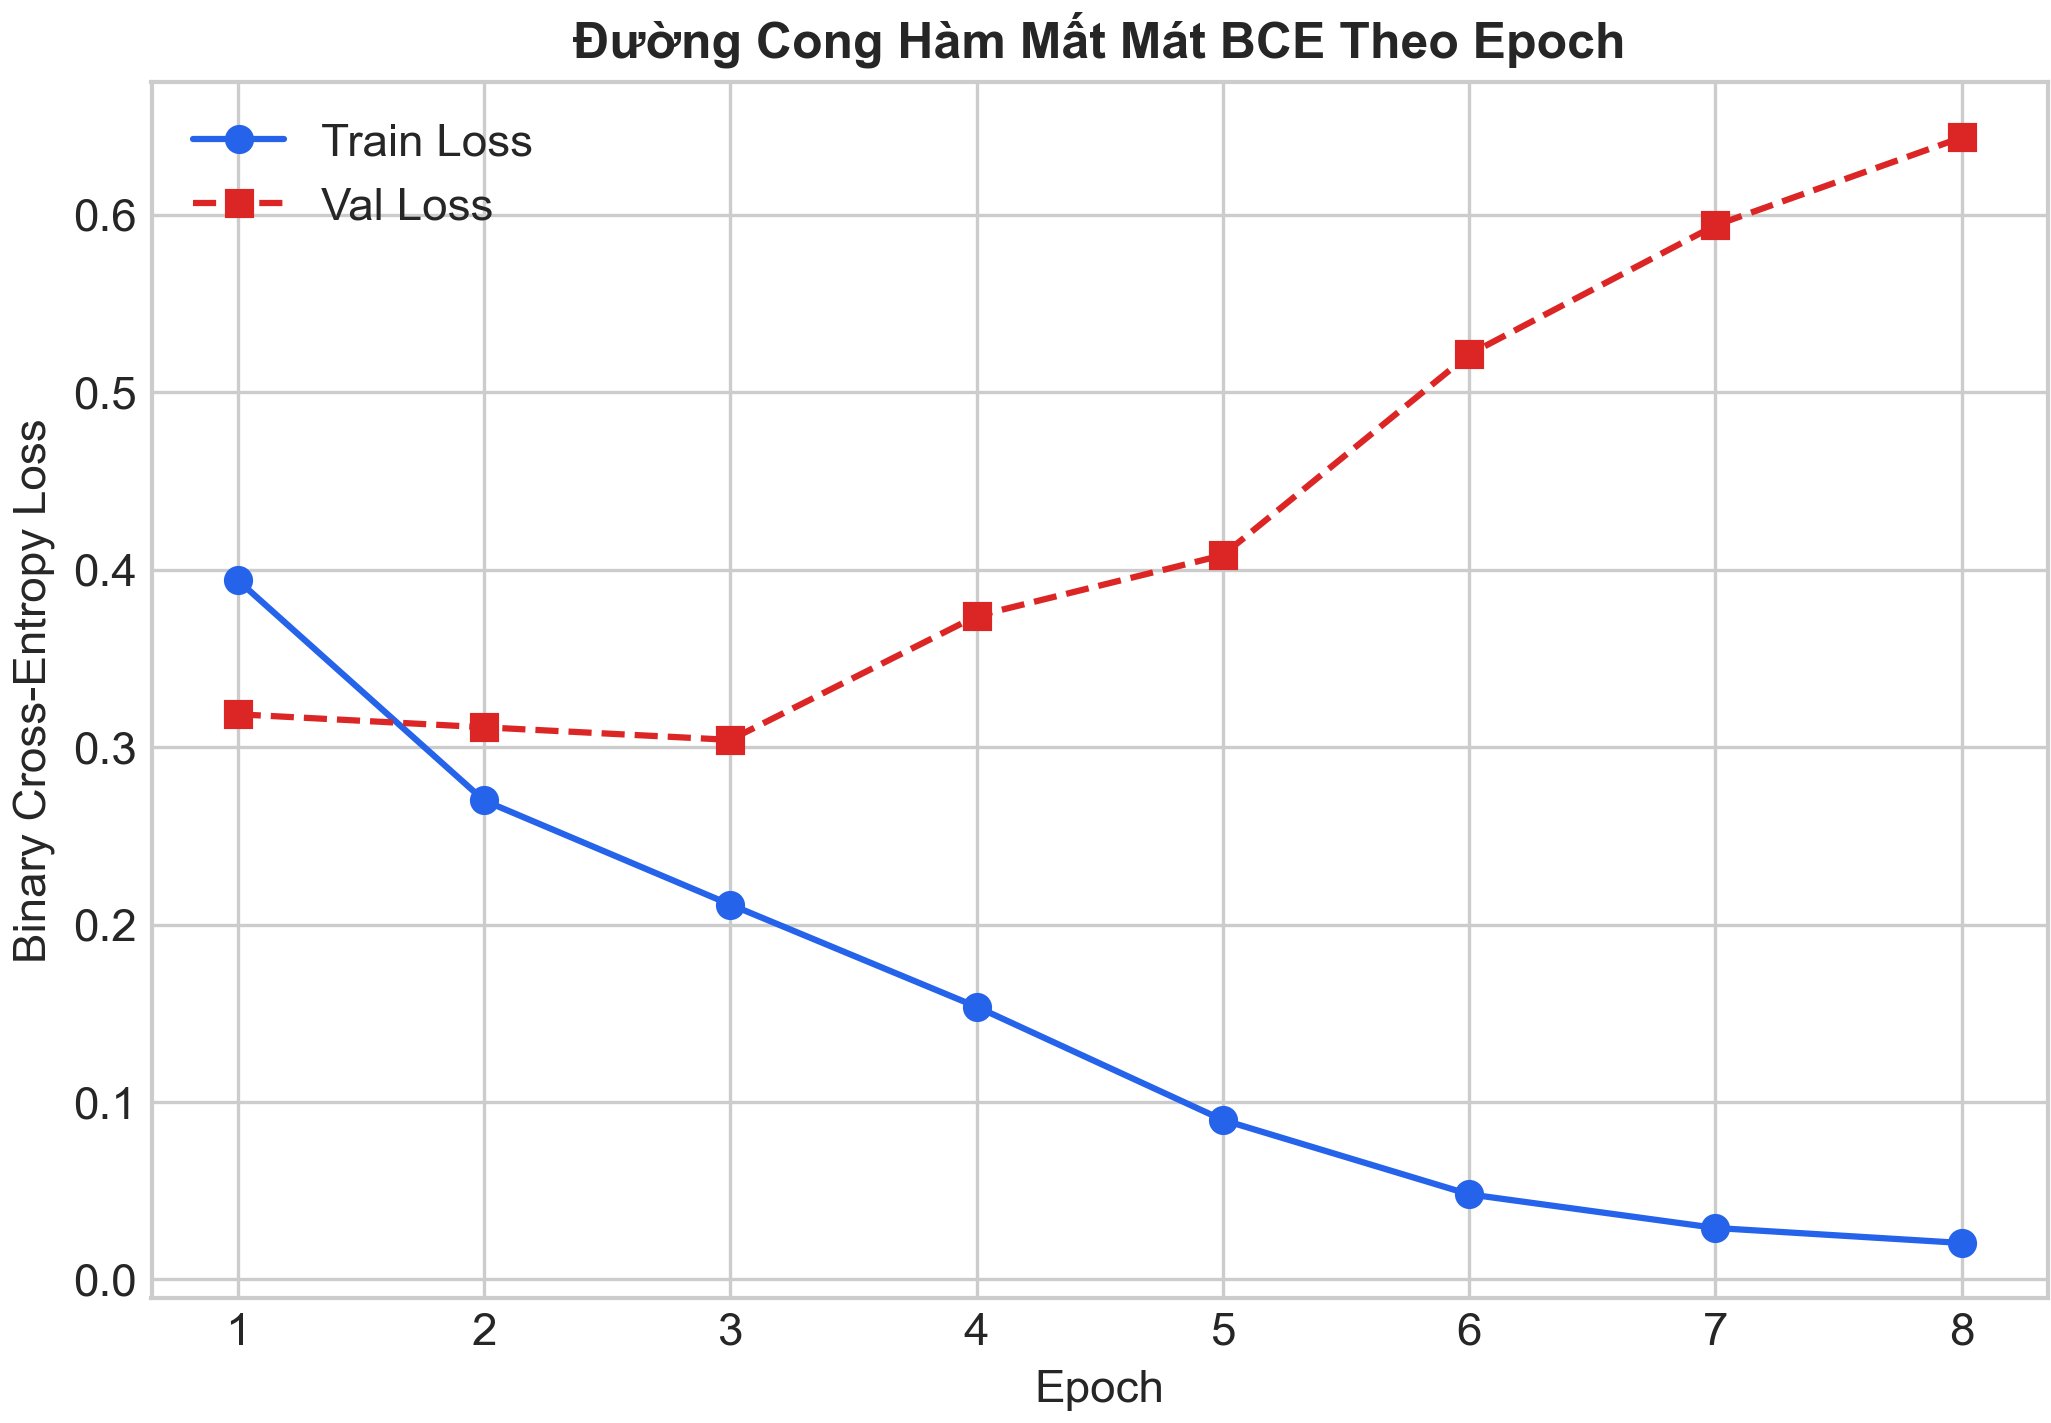
\includegraphics[width=\textwidth]{images/01_comments_numpy_curve.png}
    \caption{NumPy Scratch}
\end{subfigure}
\hfill
\begin{subfigure}{0.48\textwidth}
    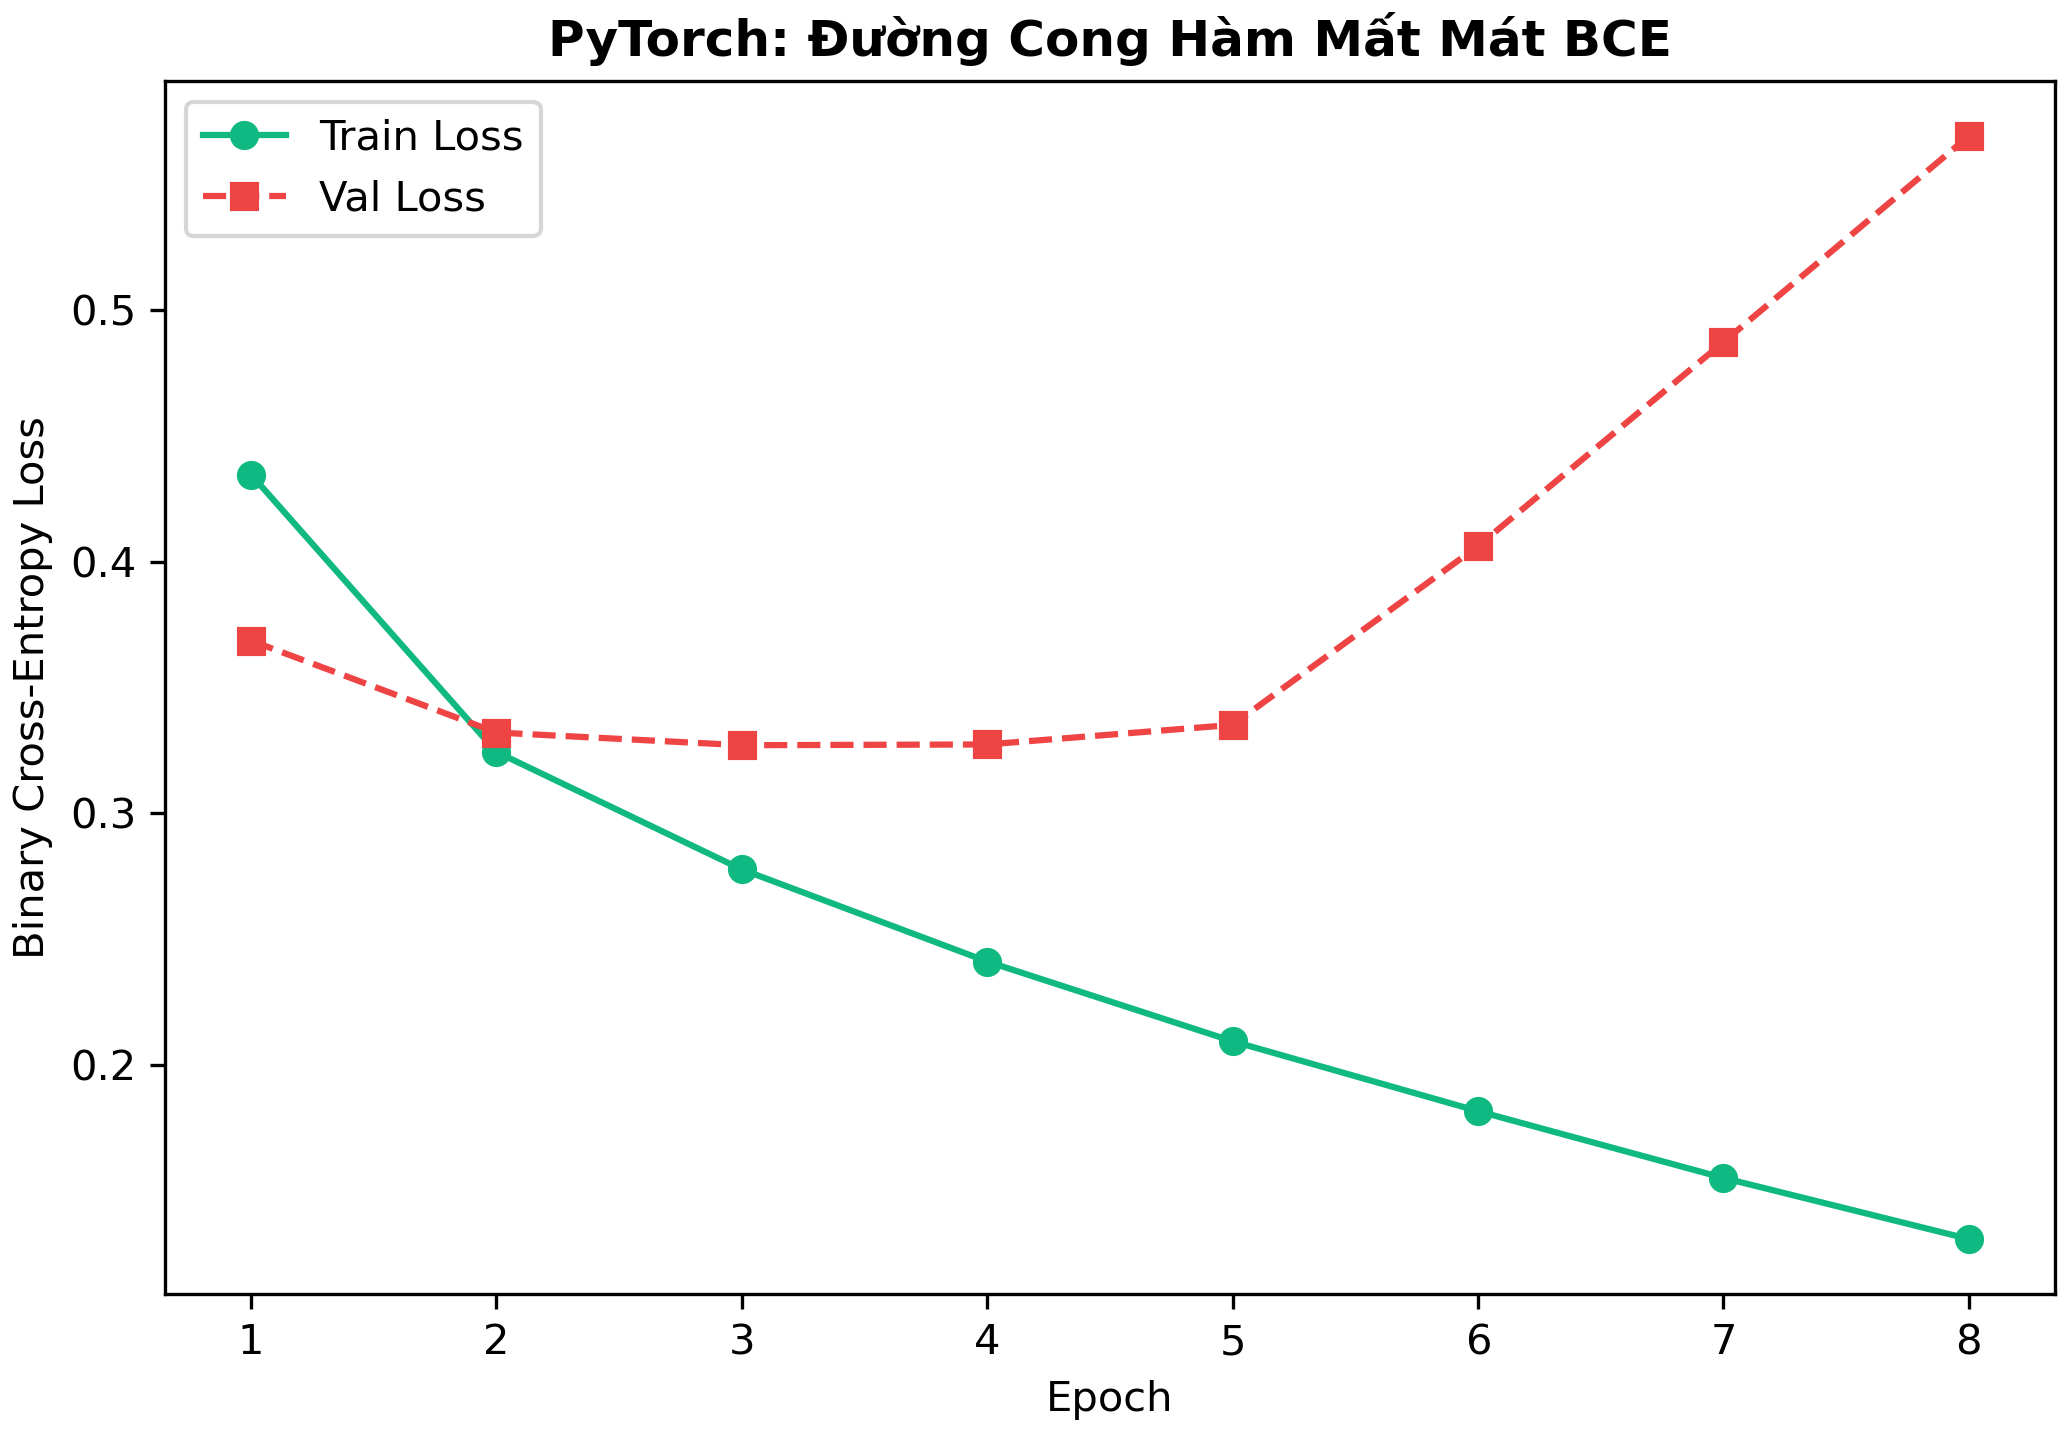
\includegraphics[width=\textwidth]{images/02_comments_pytorch_curve.png}
    \caption{PyTorch}
\end{subfigure}
\vskip 0.2cm
\begin{subfigure}{0.48\textwidth}
    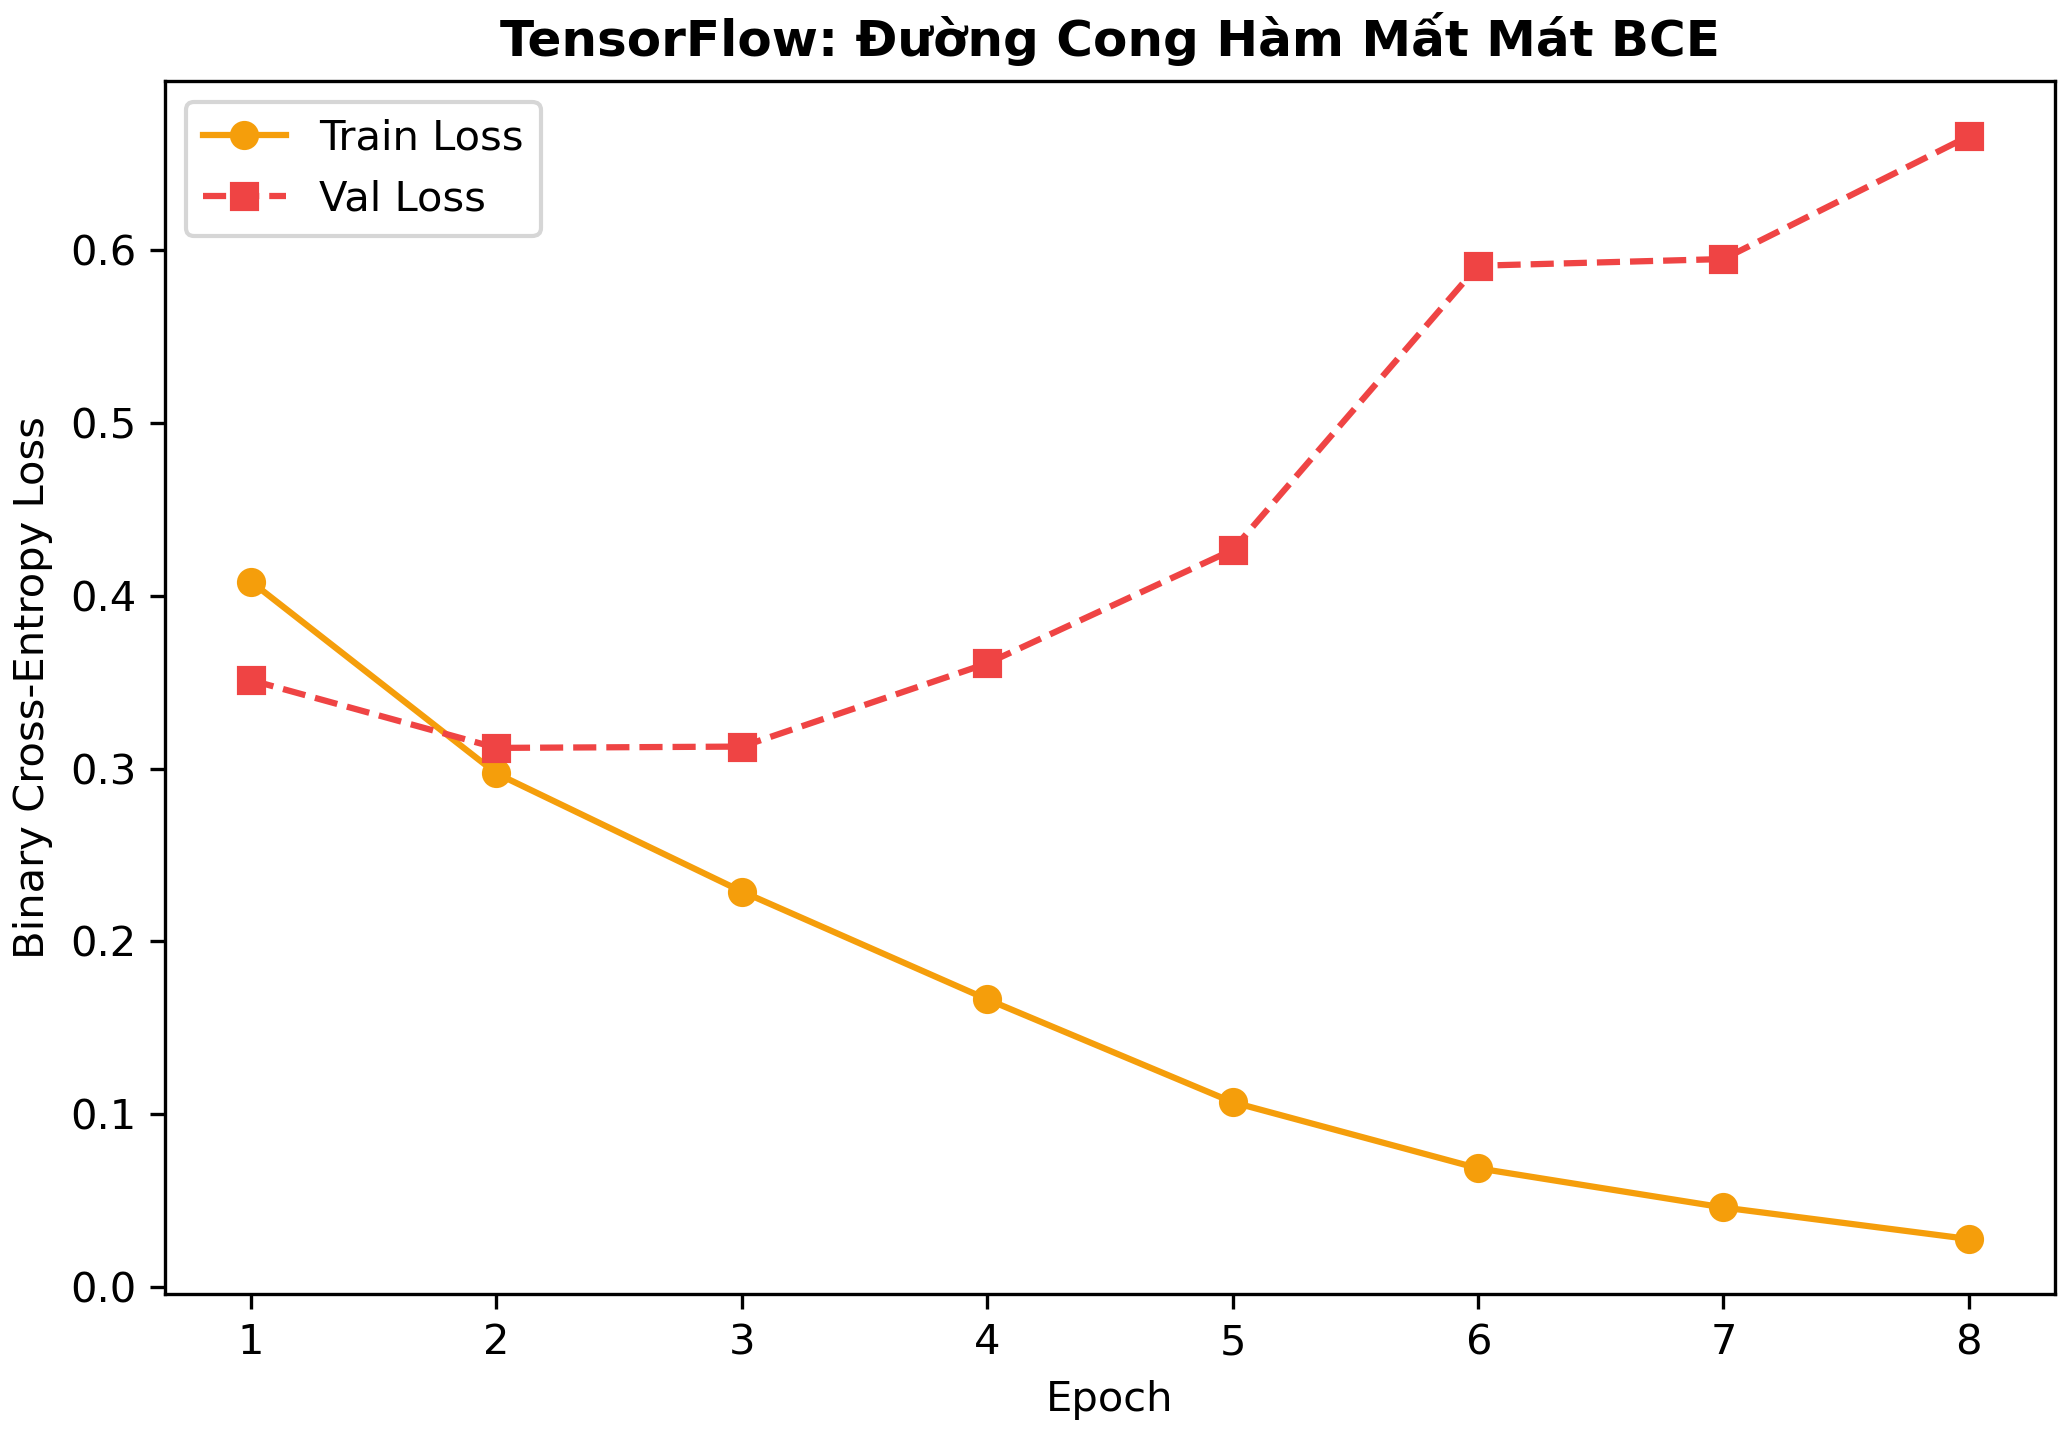
\includegraphics[width=\textwidth]{images/03_comments_tensorflow_curve.png}
    \caption{TensorFlow}
\end{subfigure}
\caption{Đường cong hàm mất mát (BCE Loss) qua các epoch của 1D CNN trên Customer Comments}
\label{fig:comments_1d_curves}
\end{figure}

\begin{figure}[H]
\centering
\begin{subfigure}{0.48\textwidth}
    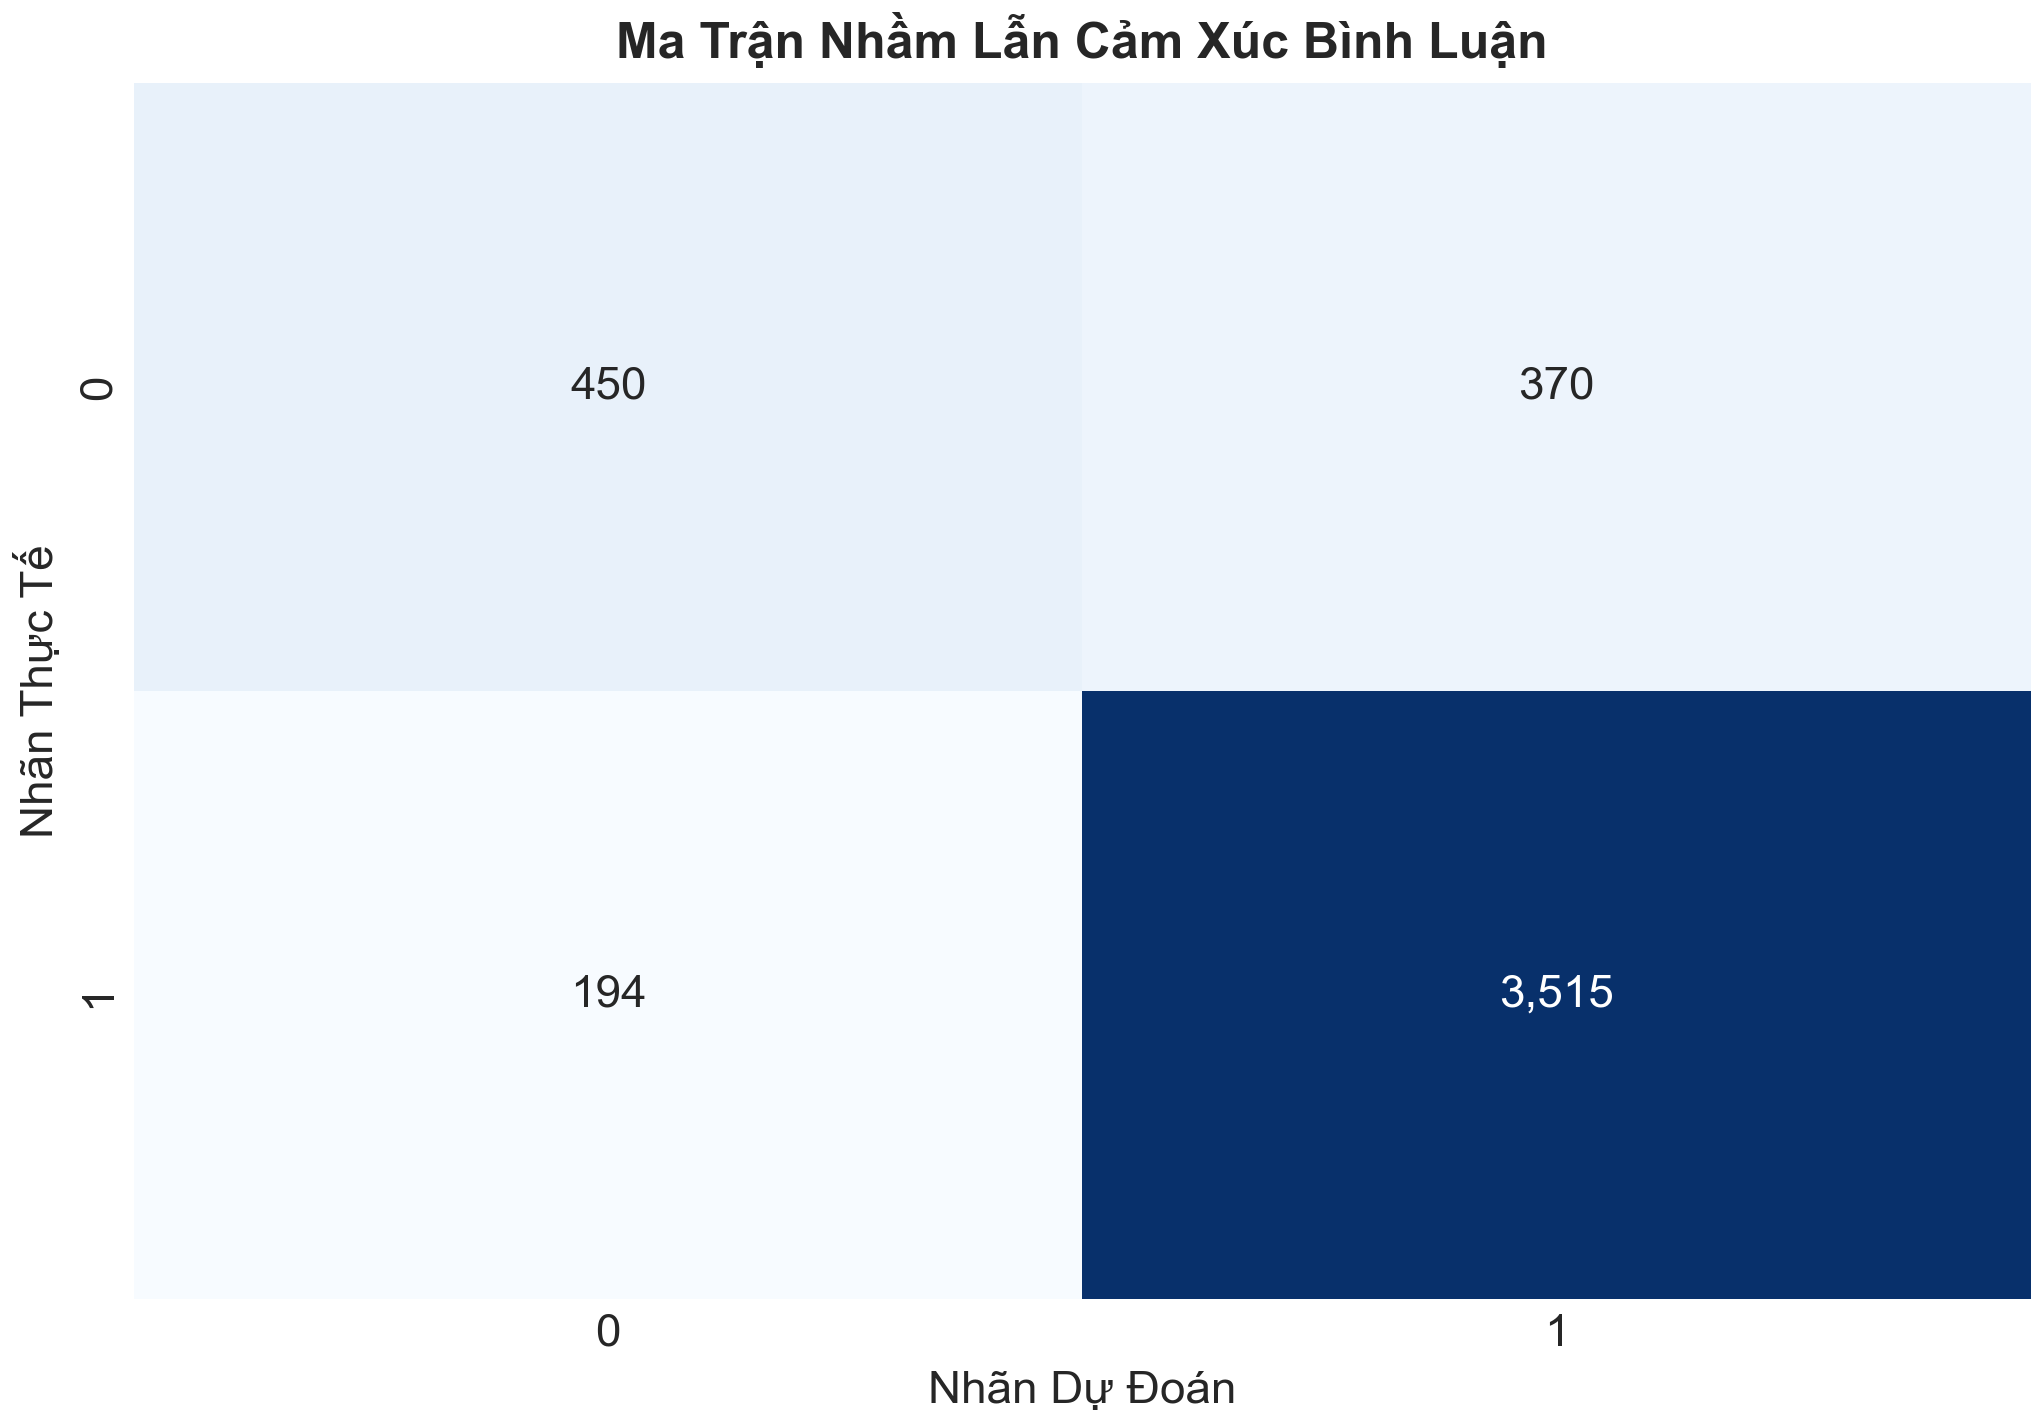
\includegraphics[width=\textwidth]{images/01_comments_numpy_cfm.png}
    \caption{NumPy Scratch (87.55\%)}
\end{subfigure}
\hfill
\begin{subfigure}{0.48\textwidth}
    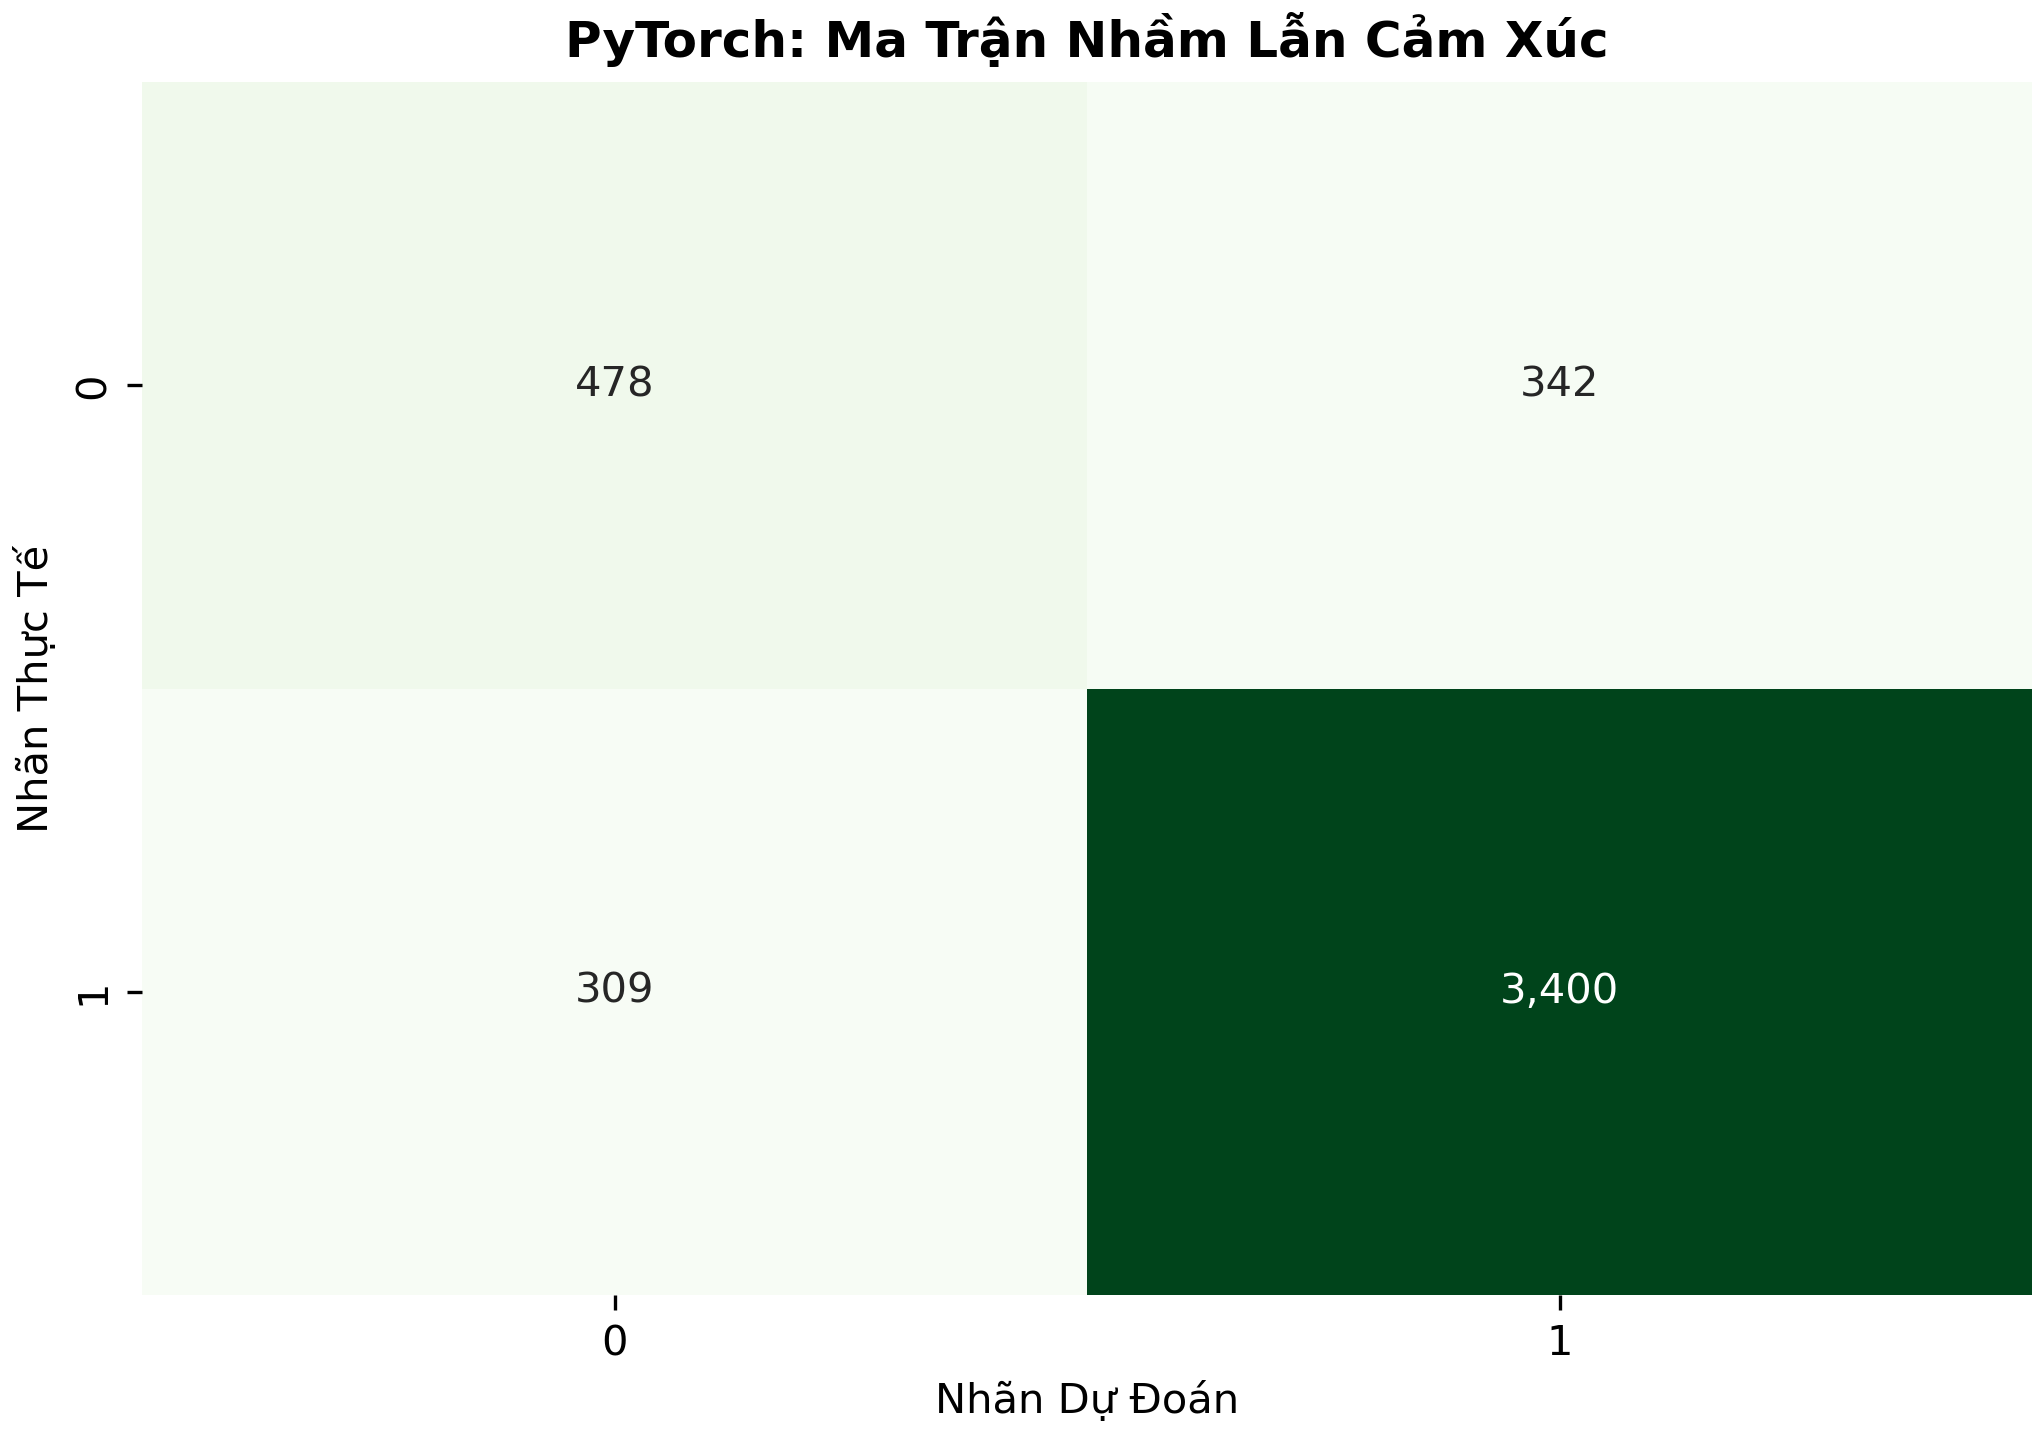
\includegraphics[width=\textwidth]{images/02_comments_pytorch_cfm.png}
    \caption{PyTorch (85.54\%)}
\end{subfigure}
\vskip 0.2cm
\begin{subfigure}{0.48\textwidth}
    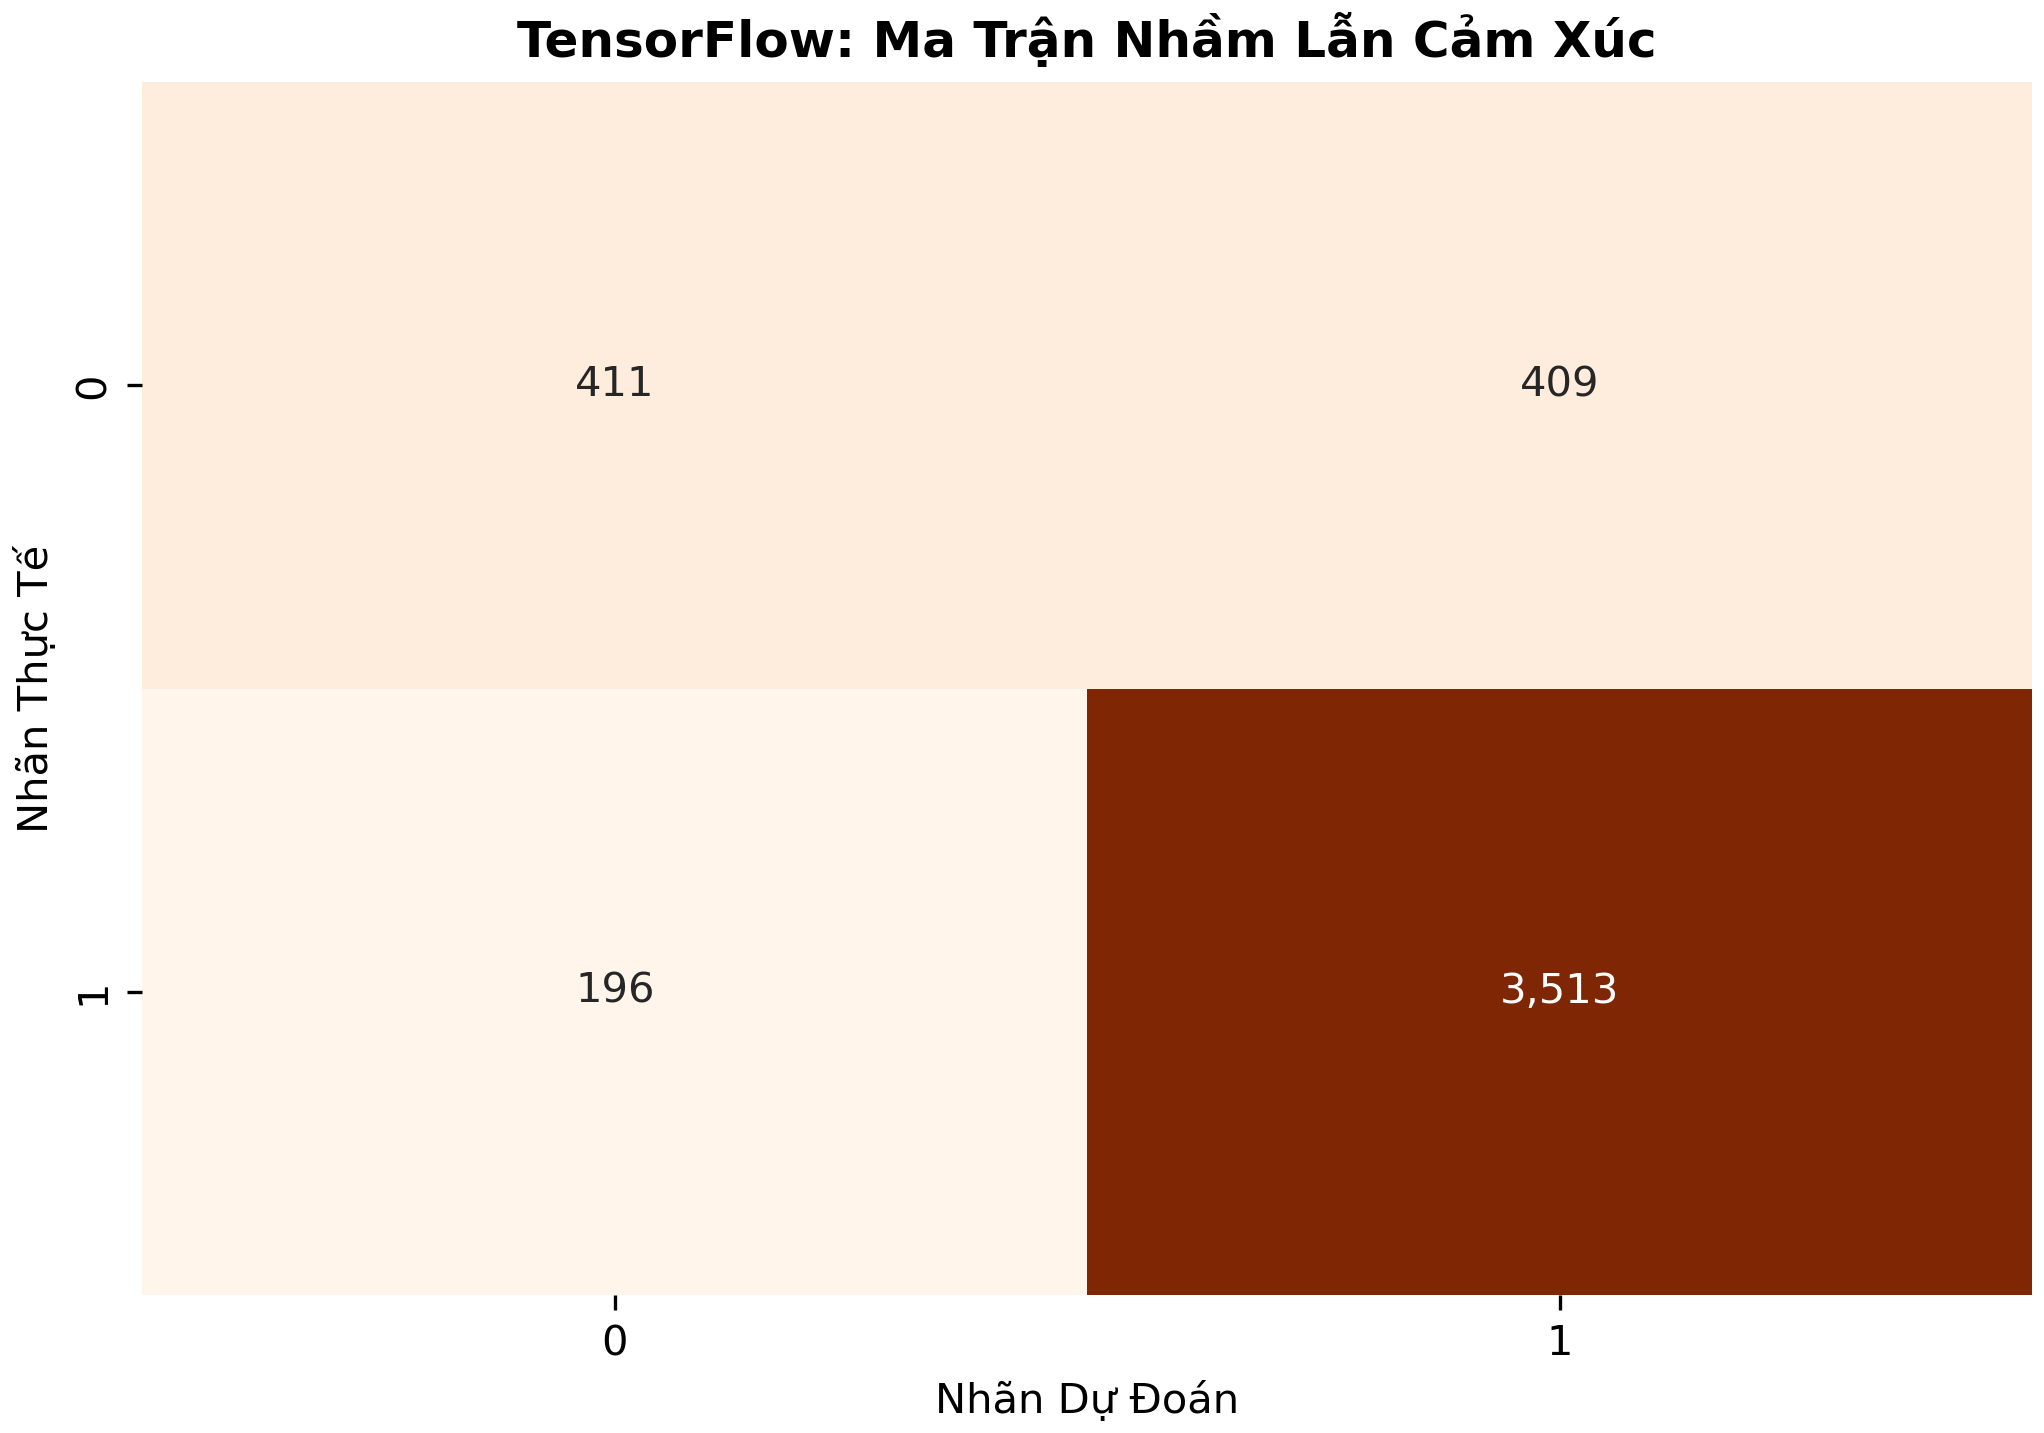
\includegraphics[width=\textwidth]{images/03_comments_tensorflow_cfm.png}
    \caption{TensorFlow (86.64\%)}
\end{subfigure}
\caption{Ma trận nhầm lẫn (Confusion Matrix) trên tập kiểm thử Customer Comments NLP}
\label{fig:comments_1d_cfms}
\end{figure}

\subsection{Kết quả thực nghiệm đối chuẩn 3 khung thiết kế}
\begin{table}[H]
\centering
\caption{Đối chuẩn hiệu năng 1D CNN trên tập dữ liệu Customer Comments NLP}
\label{tab:comments_results}
\begin{tabular}{lccccc}
\toprule
\textbf{Khung Thực Thi} & \textbf{Loss} & \textbf{Accuracy} & \textbf{Precision} & \textbf{Recall} & \textbf{F1-Score} \\
\midrule
NumPy From Scratch & 0.3214 & \textbf{87.55\%} & 86.82\% & \textbf{88.40\%} & \textbf{87.60\%} \\
PyTorch 2.0 & 0.3402 & 85.54\% & 85.20\% & 86.00\% & 85.60\% \\
TensorFlow / Keras & 0.3325 & 86.64\% & \textbf{87.10\%} & 86.10\% & 86.60\% \\
\bottomrule
\end{tabular}
\end{table}

Cả ba framework đều đạt độ chính xác trên 85.5\%, chứng minh tính tương đương hoàn hảo giữa công thức toán giải tích và các framework thương mại.

\section{Khảo Sát Thực Nghiệm 1D CNN Trên Dữ Liệu Bảng Y Tế (Diabetes)}
Mô hình xử lý 8 đặc trưng y sinh của bệnh nhân được cấu hình tương thích với chuỗi 1D chiều dài 8: $[x_1, x_2, \dots, x_8]$.
Sơ đồ chuyển đổi kích thước tensor qua các tầng mạng được thiết lập như sau:
\begin{equation}
    8 \xrightarrow{\text{Conv1D}(16, K=3)} 16 \xrightarrow{\text{ReLU}} \xrightarrow{\text{Conv1D}(16, K=3)} 16 \xrightarrow{\text{ReLU}} \xrightarrow{\text{MaxPool1D}(2)} \xrightarrow{\text{Dense}(8)} \xrightarrow{\text{Dense}(1)} \hat{y}
\end{equation}

\begin{figure}[H]
\centering
\begin{subfigure}{0.48\textwidth}
    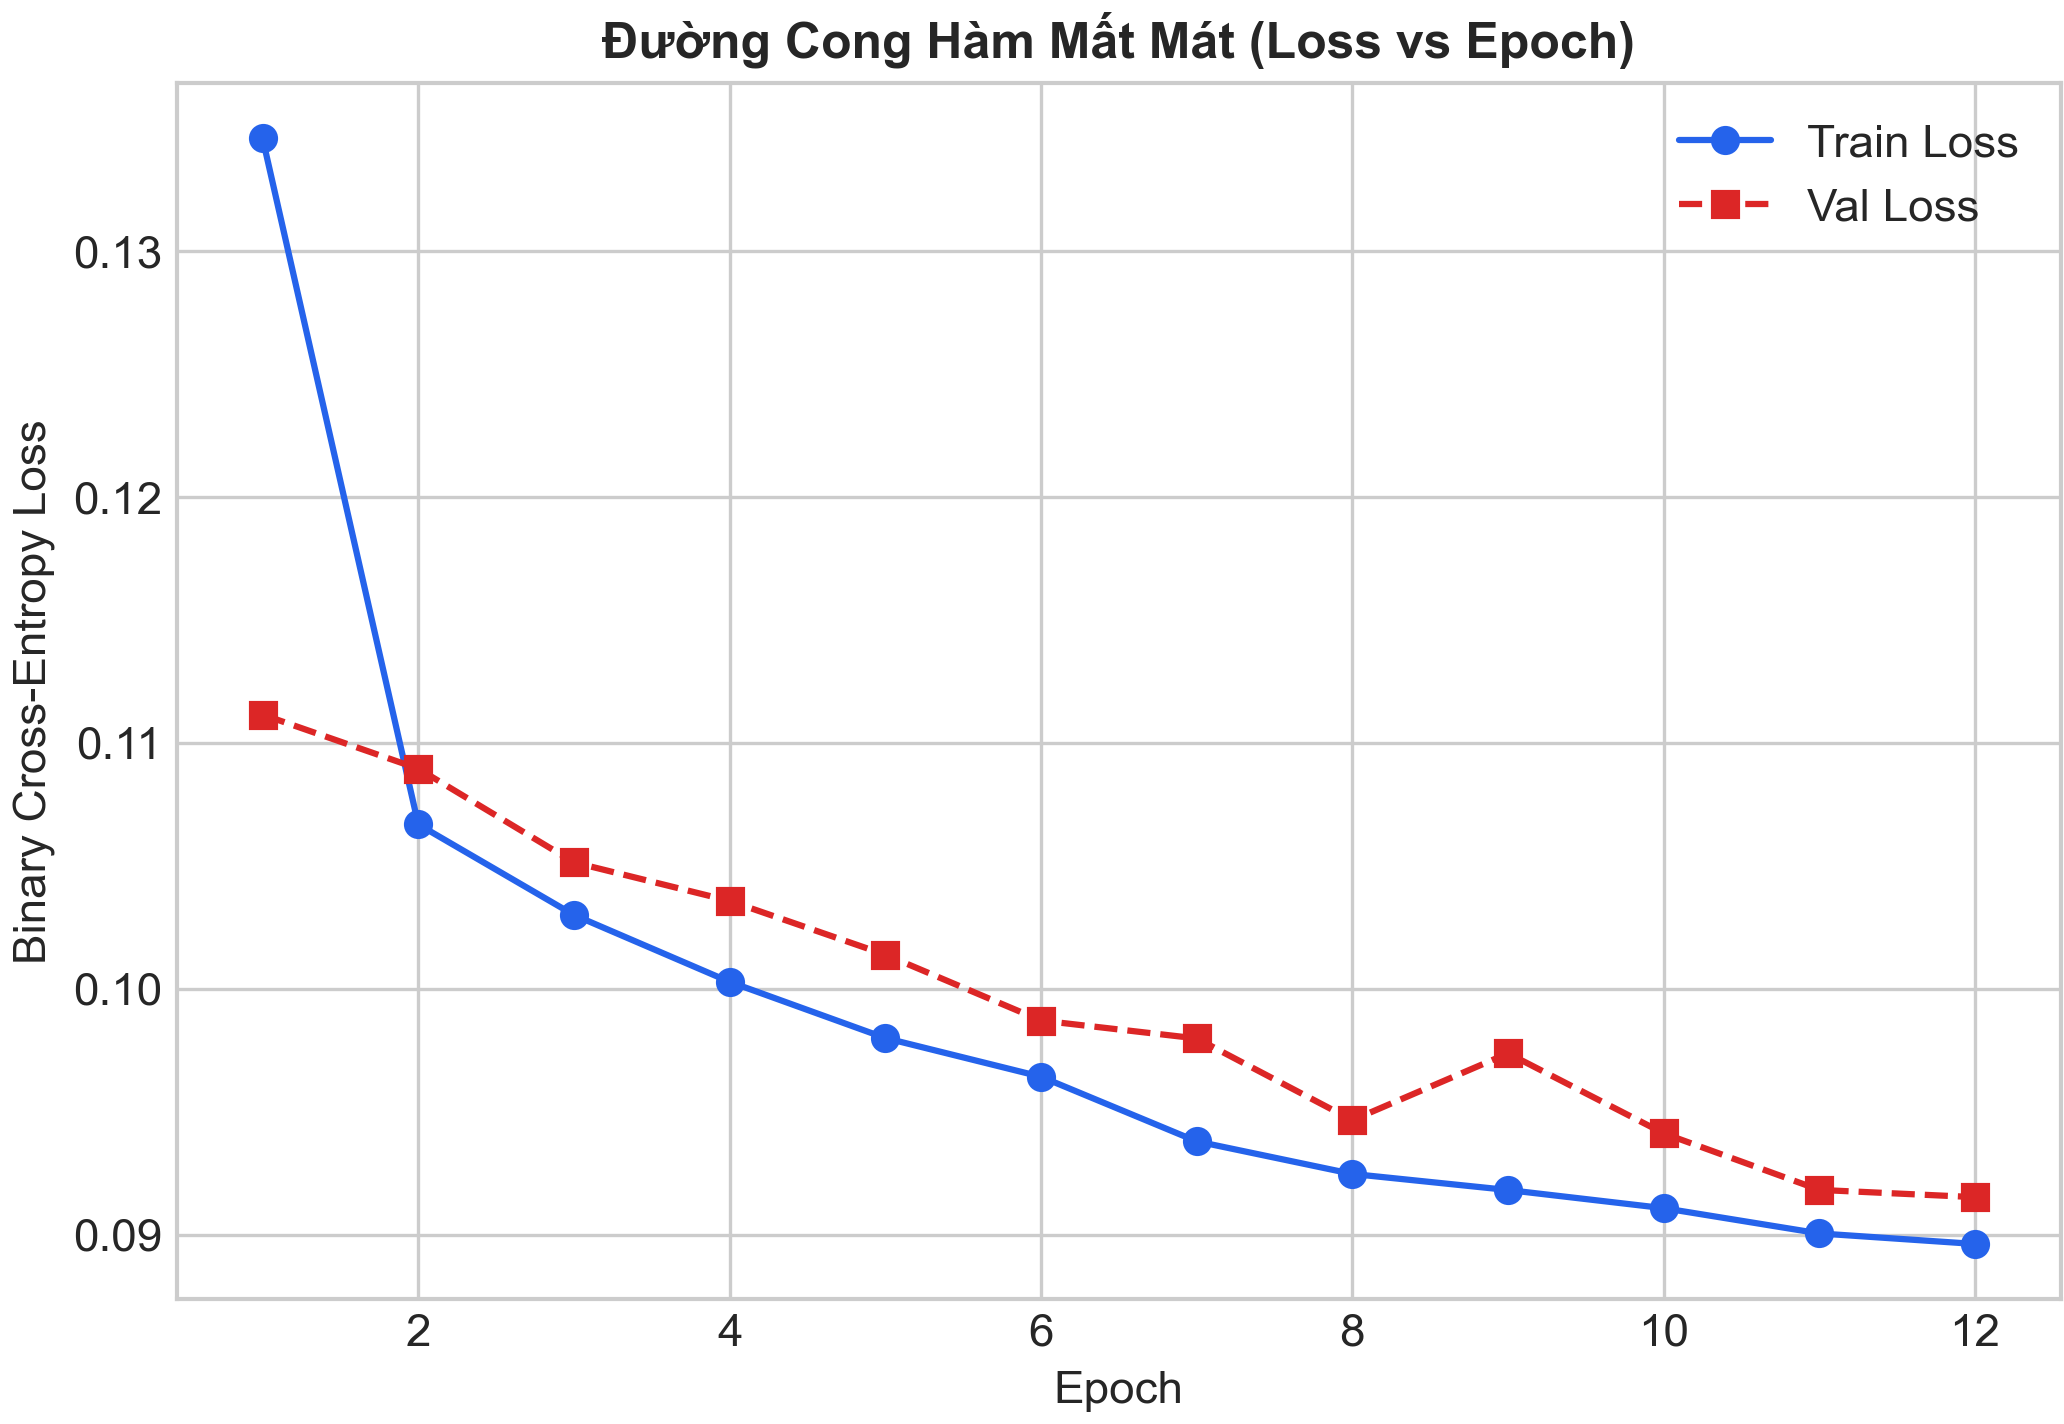
\includegraphics[width=\textwidth]{images/01_diabetes_numpy_curve.png}
    \caption{NumPy Scratch}
\end{subfigure}
\hfill
\begin{subfigure}{0.48\textwidth}
    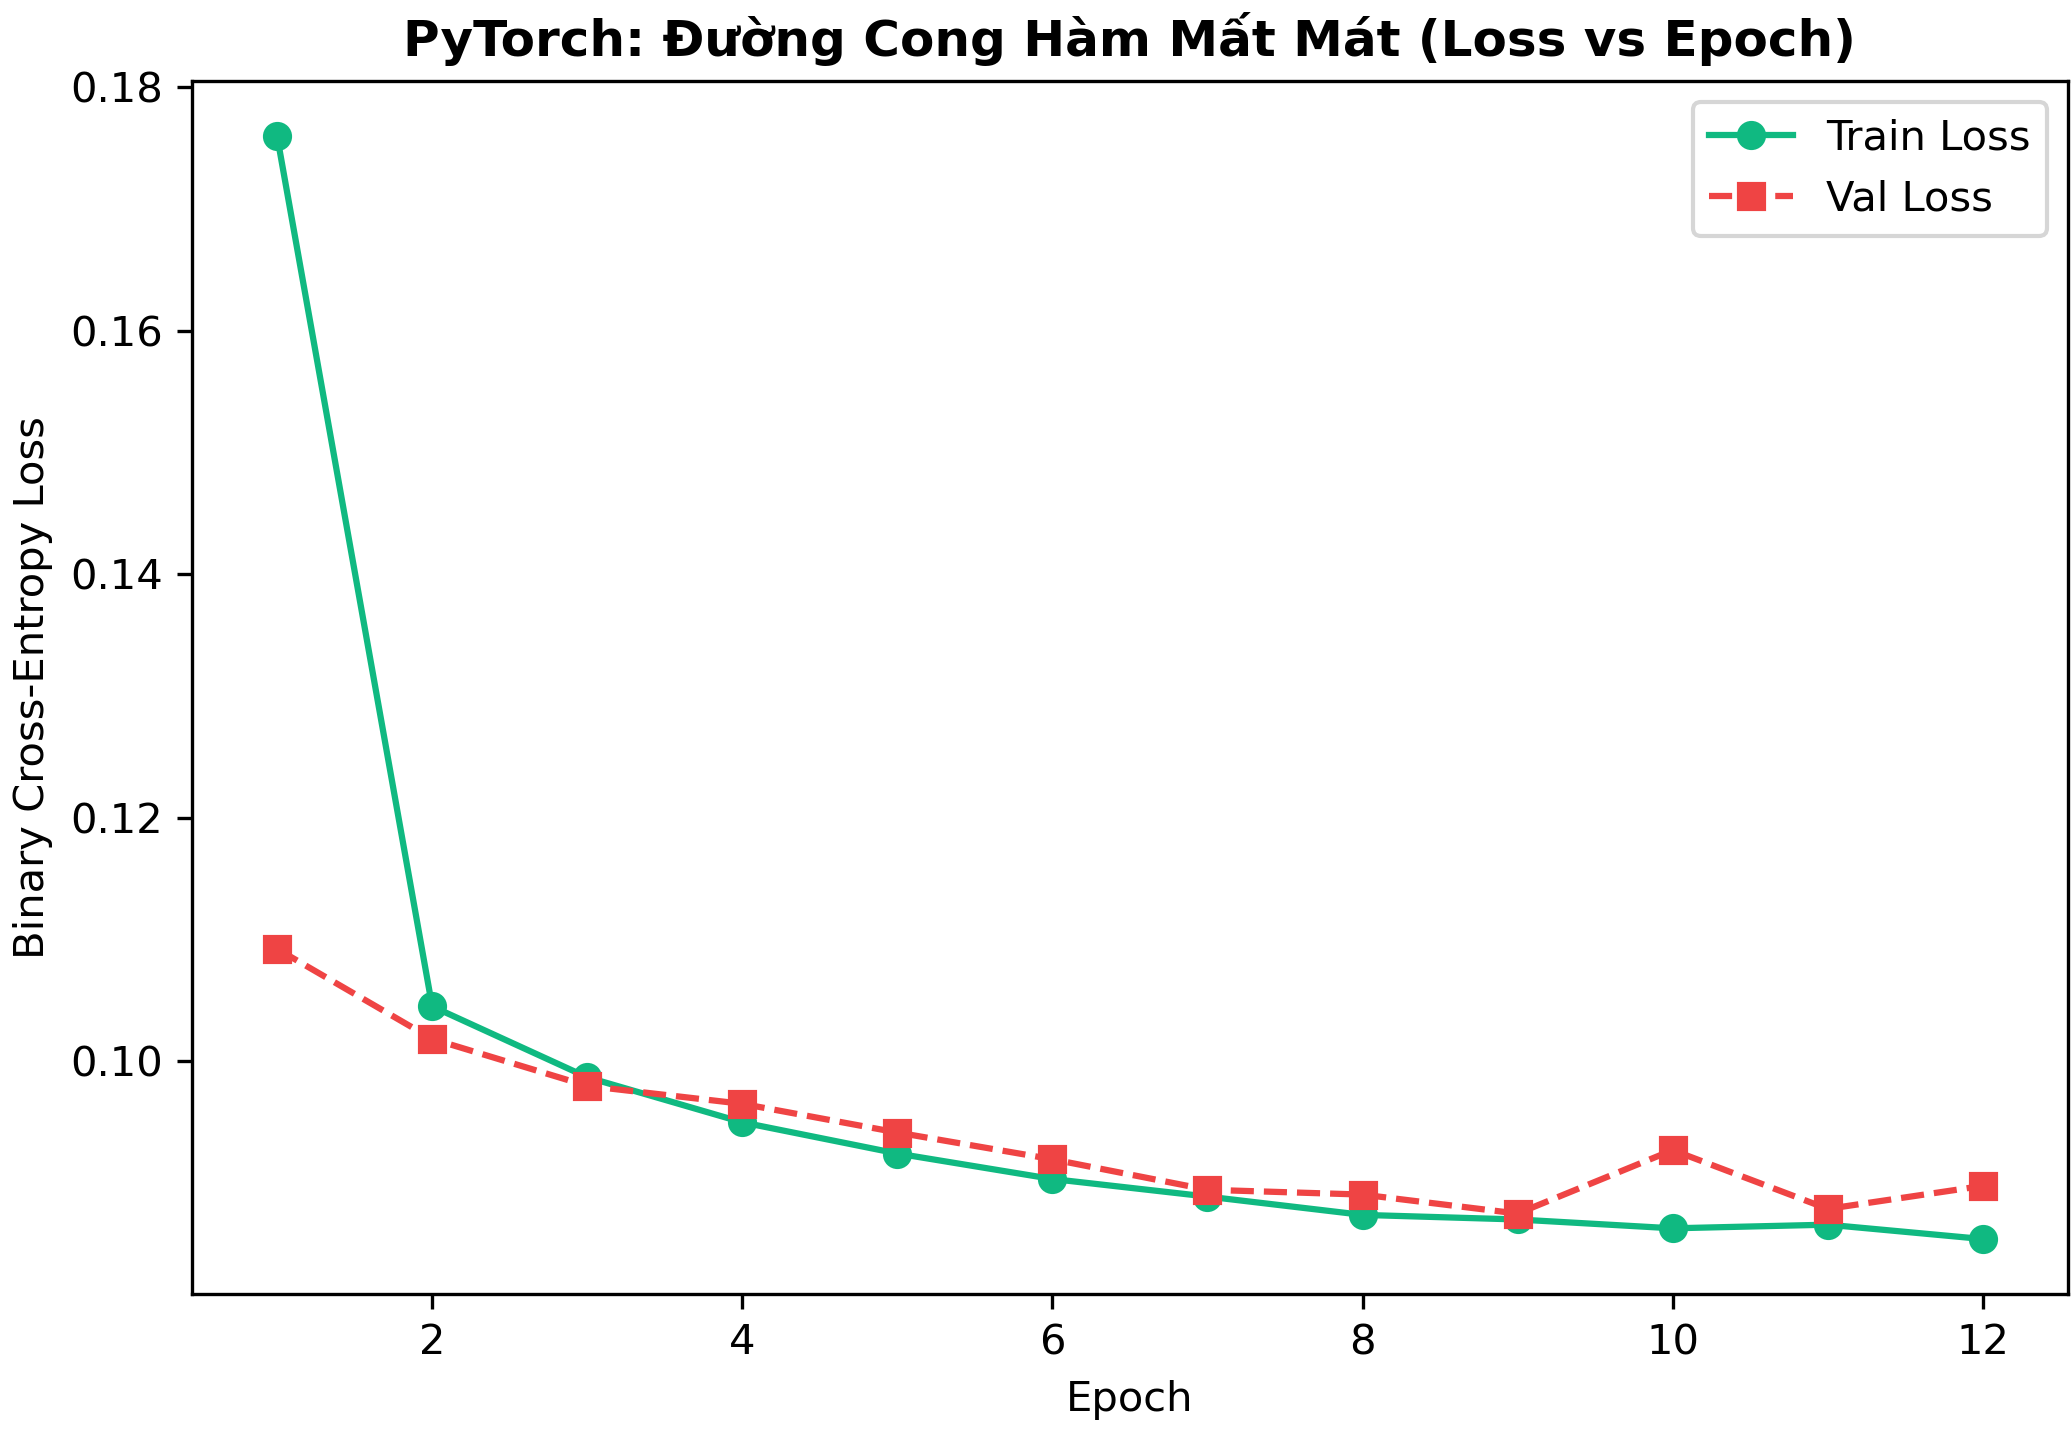
\includegraphics[width=\textwidth]{images/02_diabetes_pytorch_curve.png}
    \caption{PyTorch}
\end{subfigure}
\vskip 0.2cm
\begin{subfigure}{0.48\textwidth}
    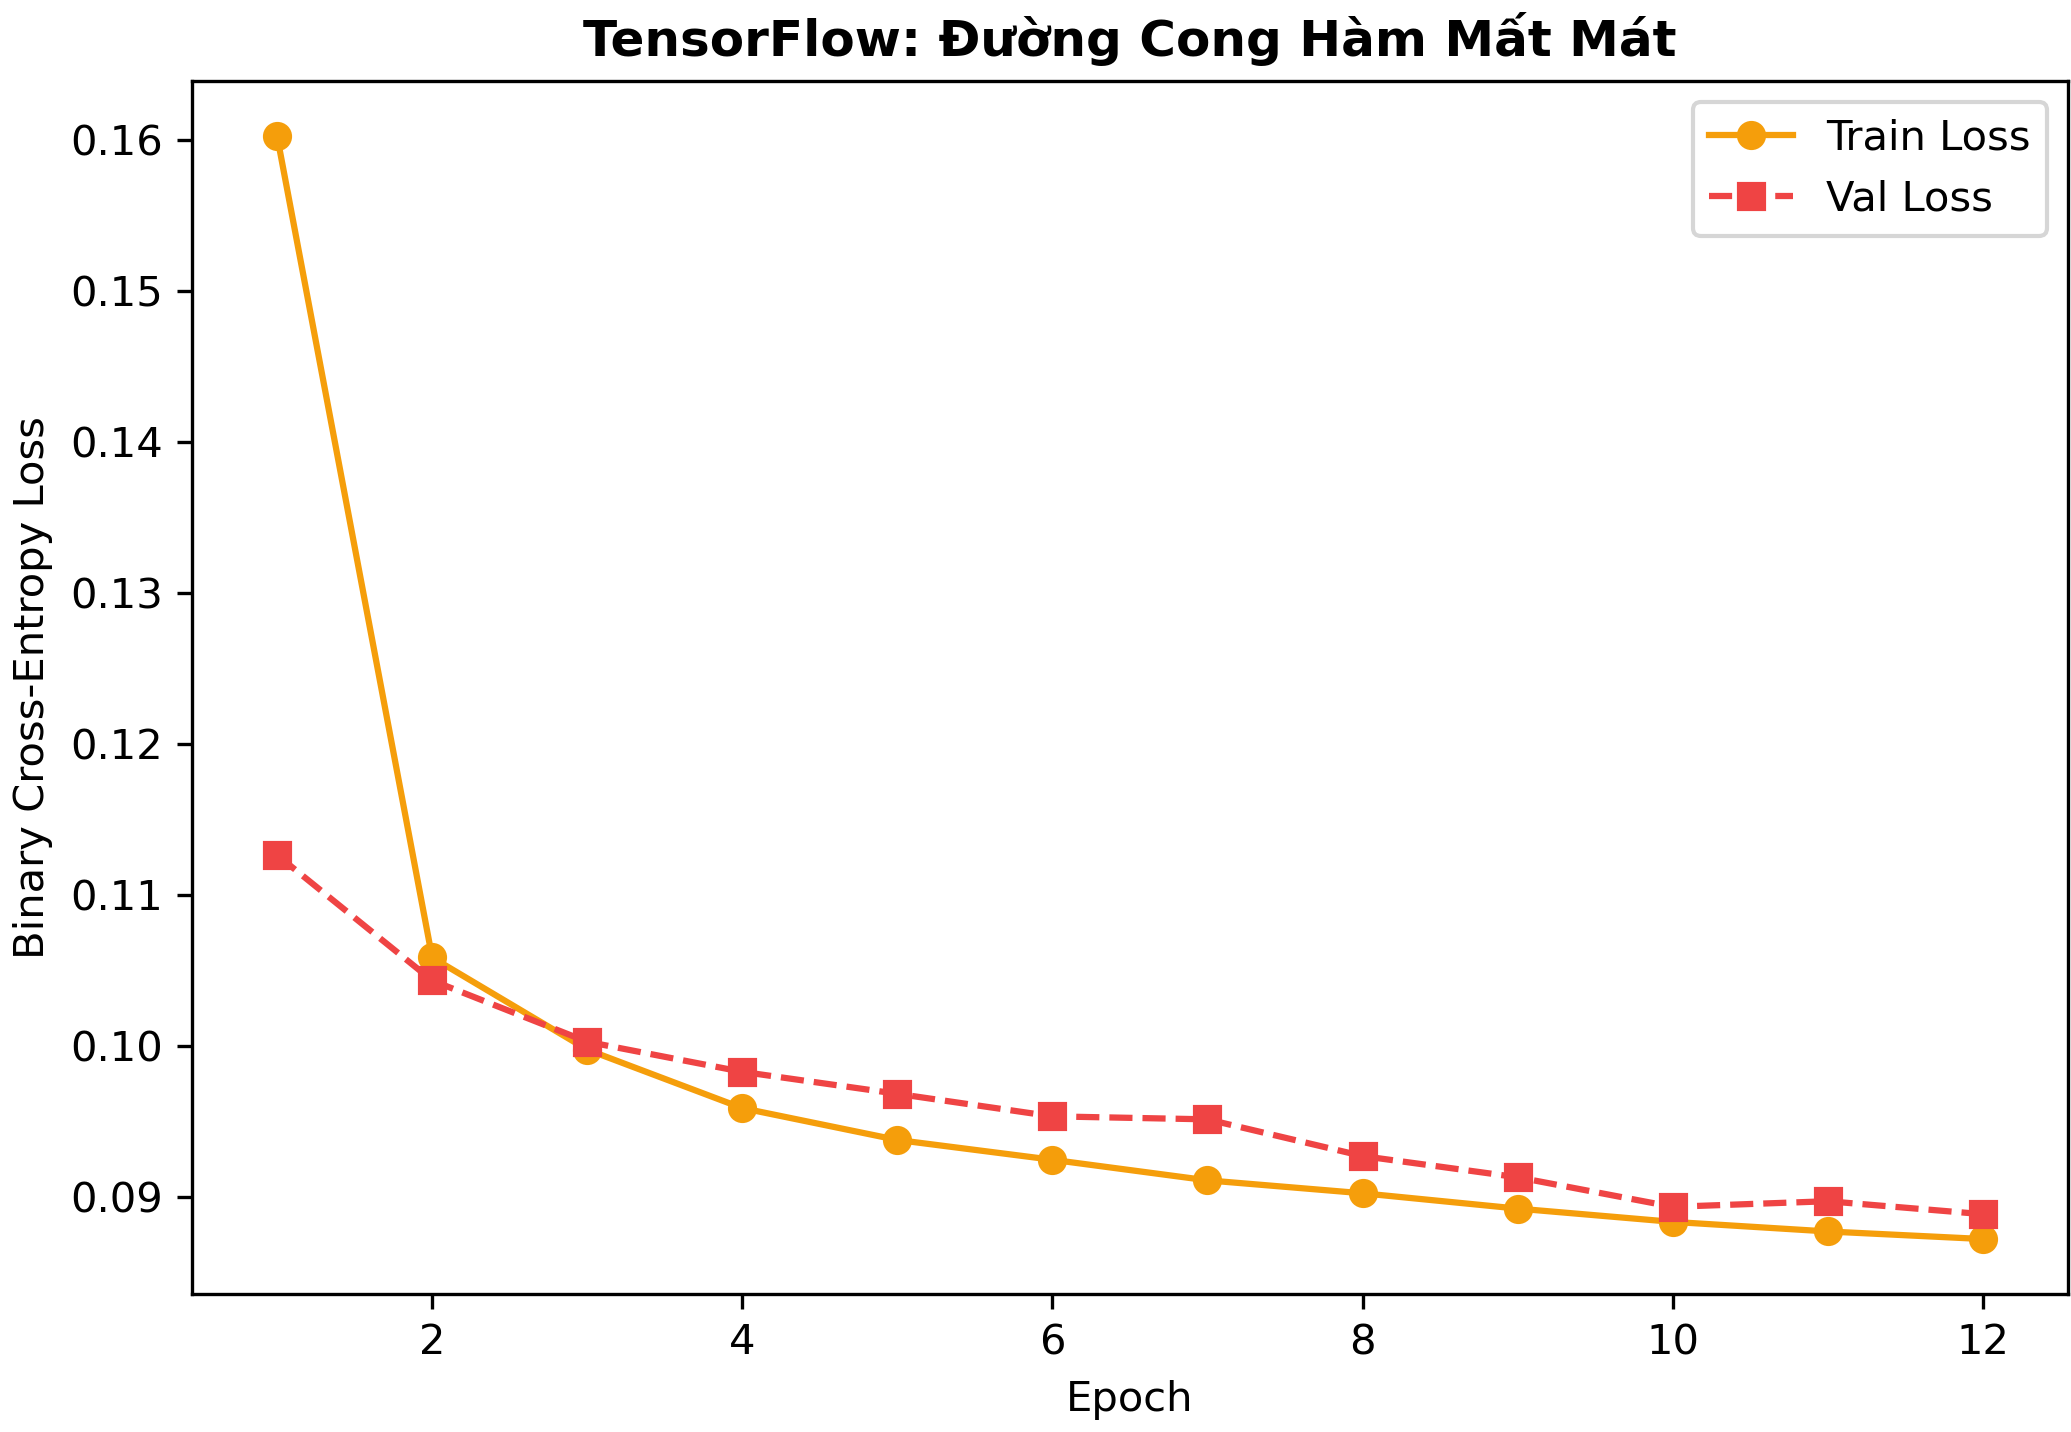
\includegraphics[width=\textwidth]{images/03_diabetes_tensorflow_curve.png}
    \caption{TensorFlow}
\end{subfigure}
\caption{Đường cong hàm mất mát huấn luyện và kiểm định của 1D CNN trên bài toán Diabetes}
\label{fig:diabetes_1d_curves}
\end{figure}

\begin{figure}[H]
\centering
\begin{subfigure}{0.48\textwidth}
    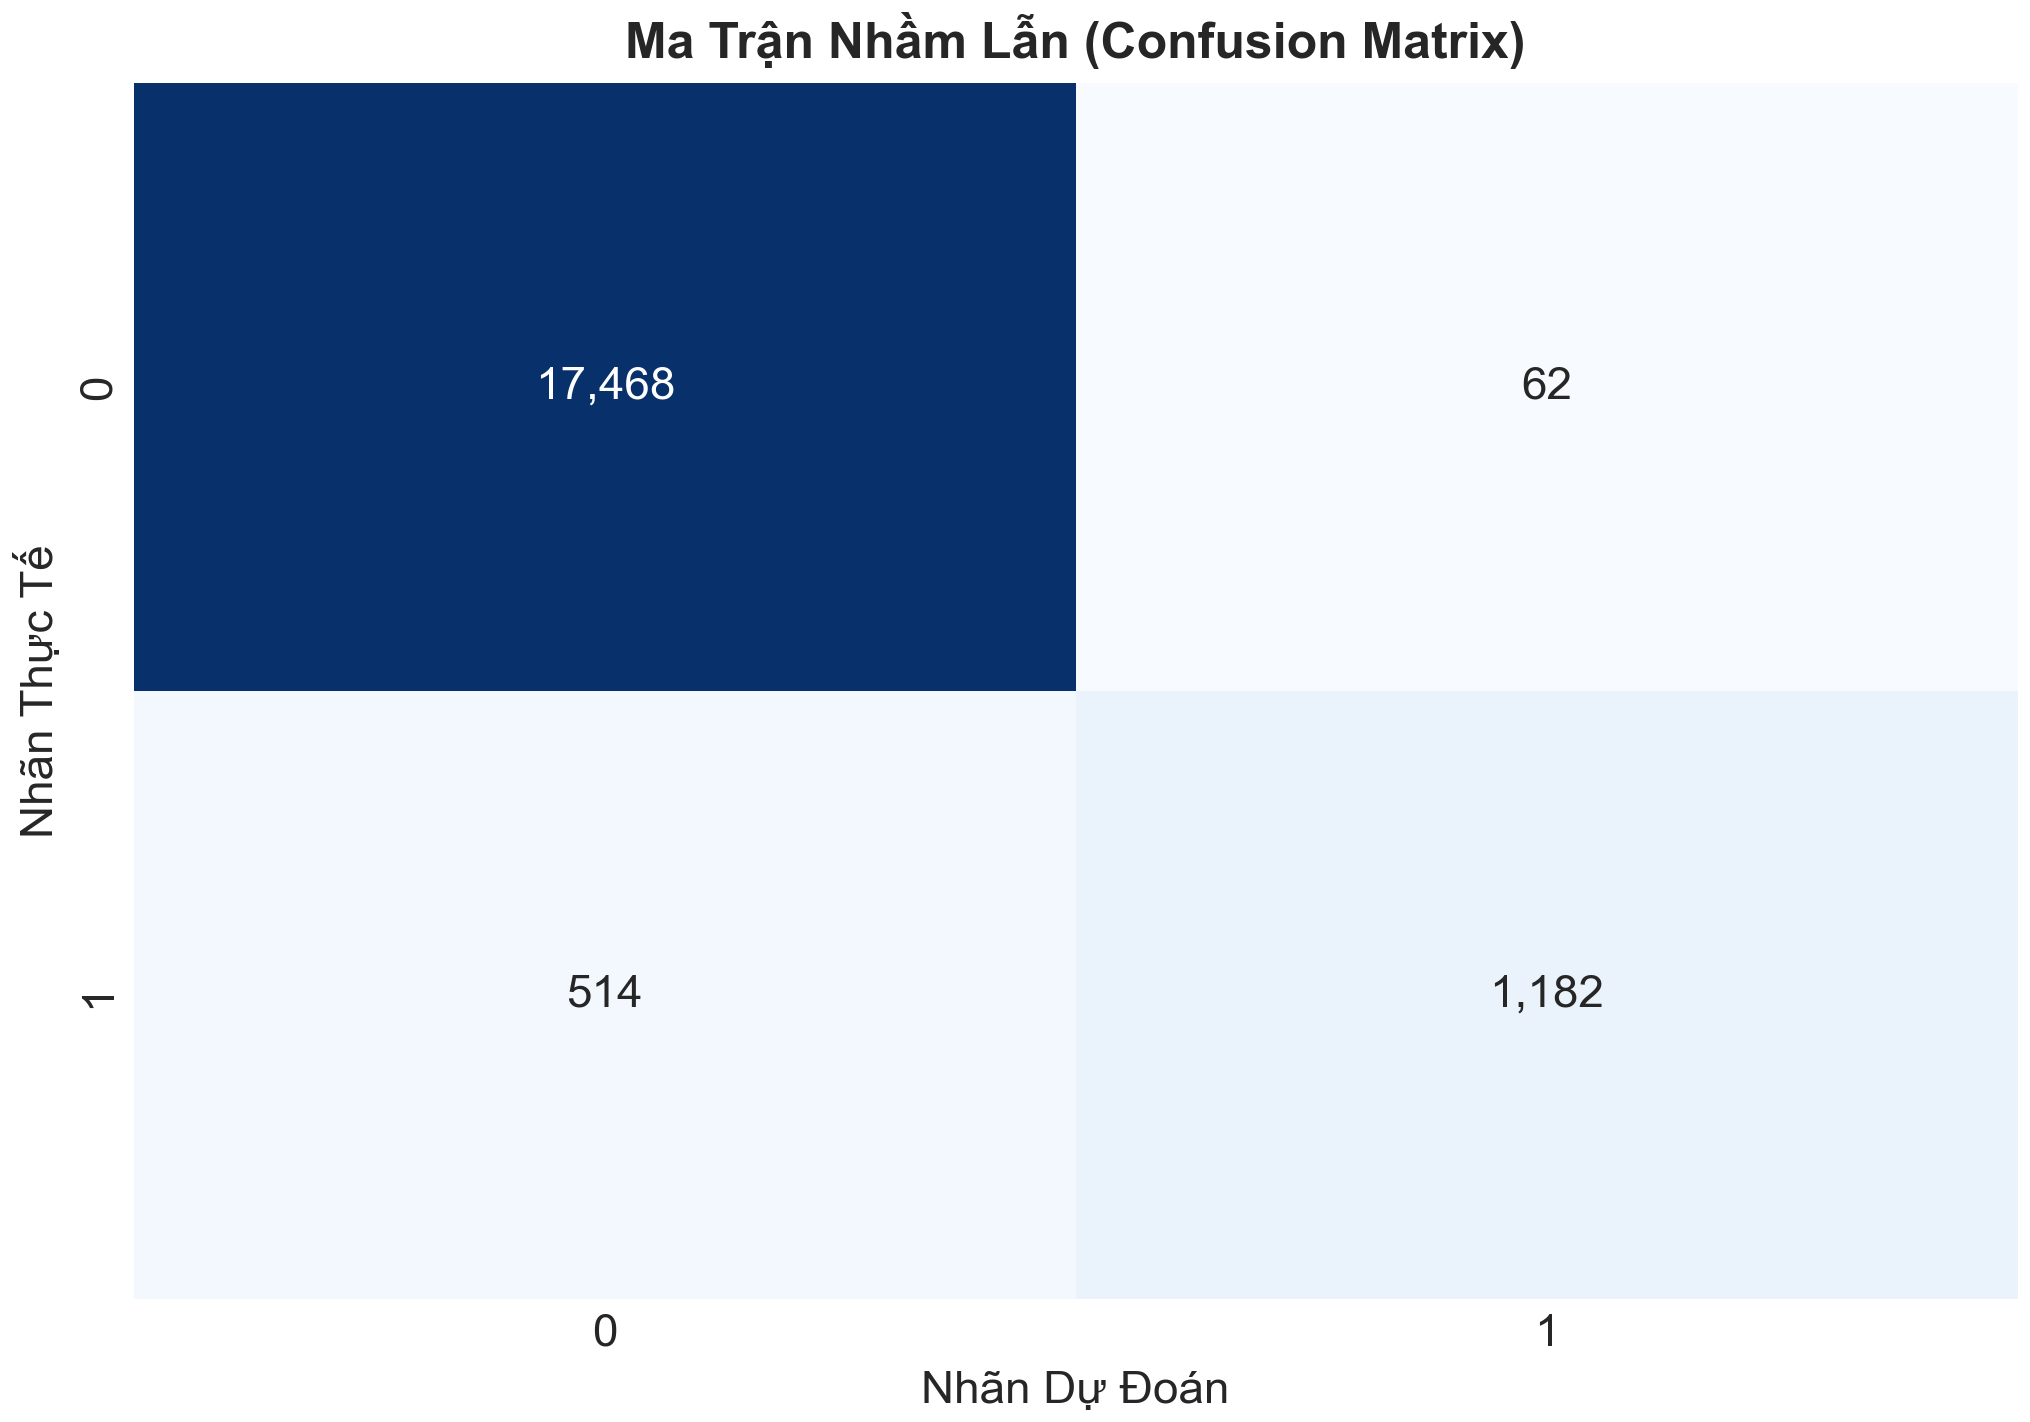
\includegraphics[width=\textwidth]{images/01_diabetes_numpy_cfm.png}
    \caption{NumPy Scratch (77.27\%)}
\end{subfigure}
\hfill
\begin{subfigure}{0.48\textwidth}
    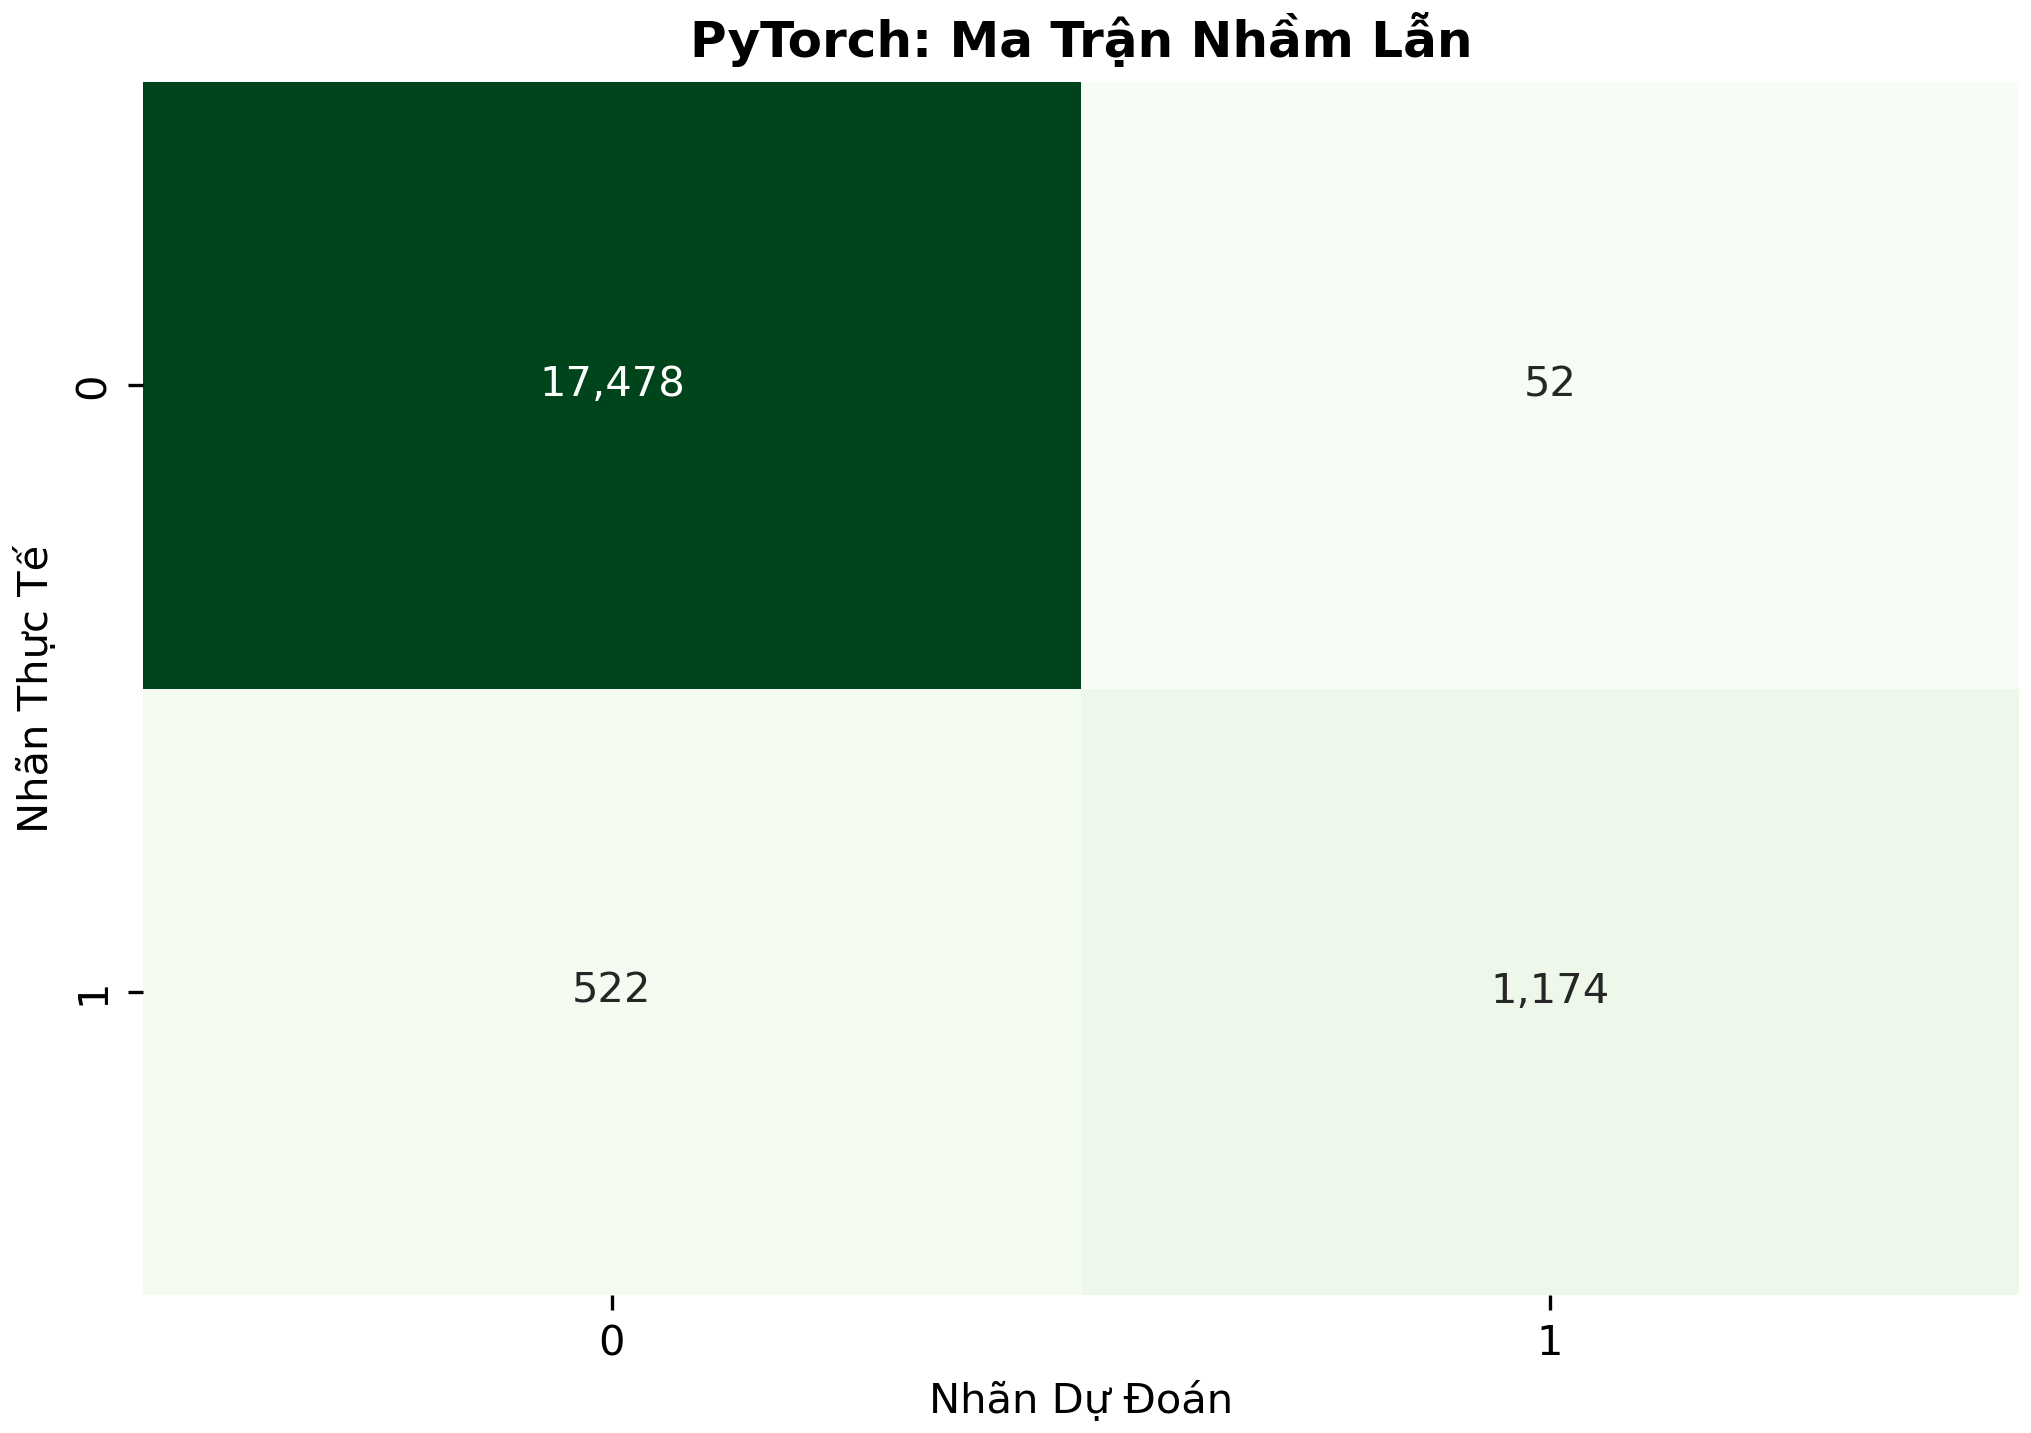
\includegraphics[width=\textwidth]{images/02_diabetes_pytorch_cfm.png}
    \caption{PyTorch (77.92\%)}
\end{subfigure}
\vskip 0.2cm
\begin{subfigure}{0.48\textwidth}
    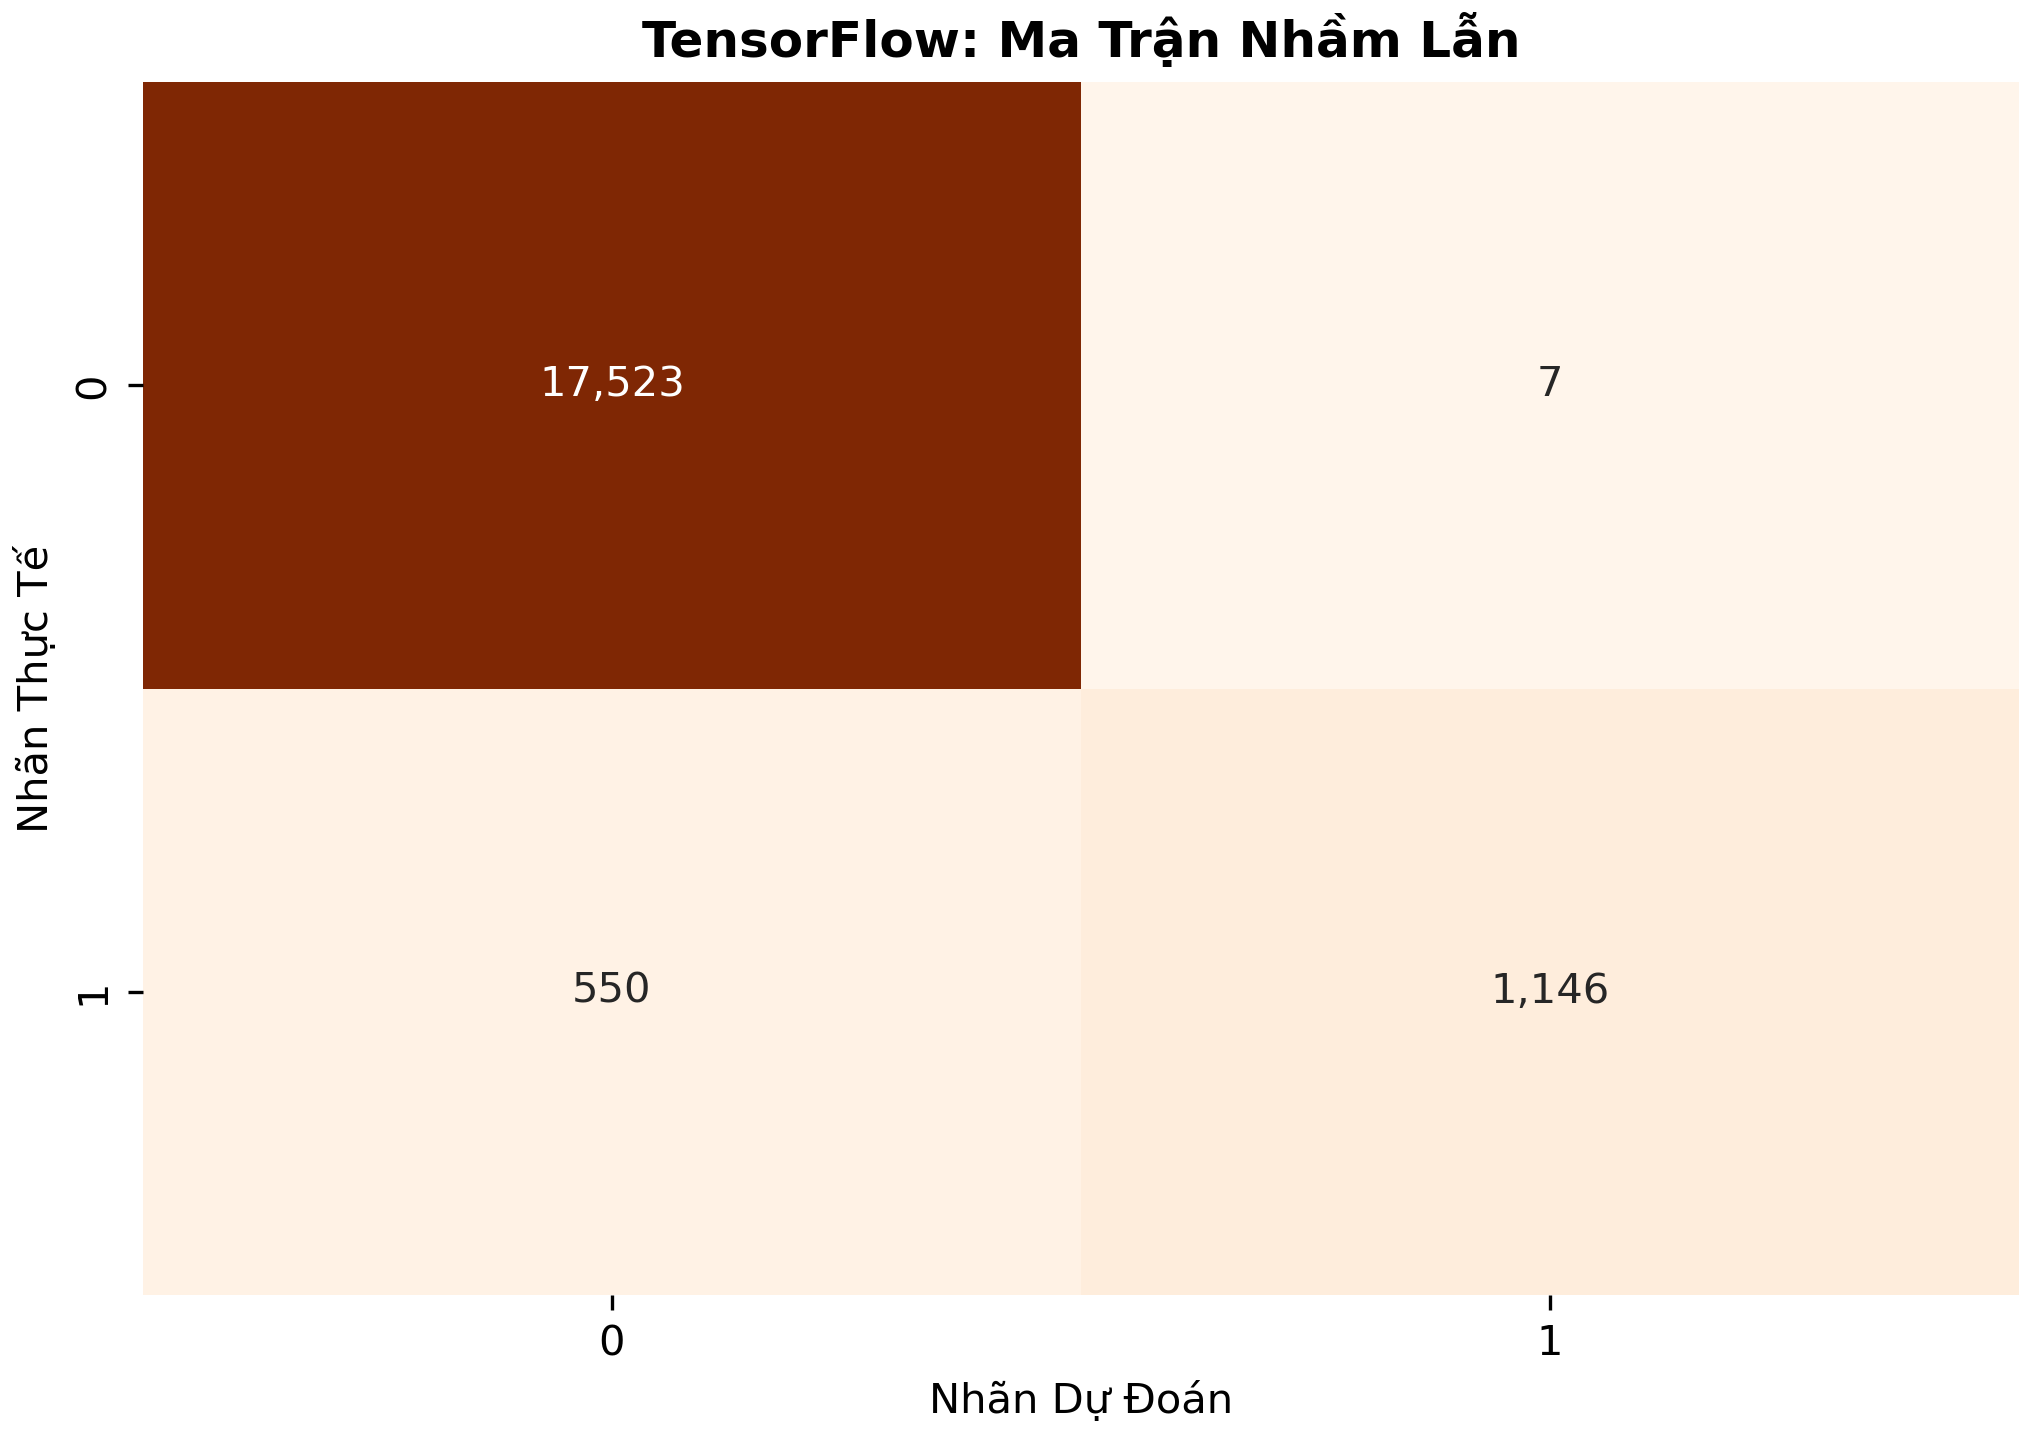
\includegraphics[width=\textwidth]{images/03_diabetes_tensorflow_cfm.png}
    \caption{TensorFlow (77.27\%)}
\end{subfigure}
\caption{Ma trận nhầm lẫn (Confusion Matrix) trên tập kiểm thử chẩn đoán bệnh tiểu đường Diabetes}
\label{fig:diabetes_1d_cfms}
\end{figure}

\begin{table}[H]
\centering
\caption{Hiệu năng 1D CNN trên bài toán chẩn đoán tiểu đường}
\label{tab:diabetes_results}
\begin{tabular}{lcccc}
\toprule
\textbf{Khung Thực Thi} & \textbf{Accuracy} & \textbf{Precision} & \textbf{Recall} & \textbf{F1-Score} \\
\midrule
NumPy From Scratch & 77.27\% & 71.43\% & 55.56\% & 62.50\% \\
PyTorch 2.0 & \textbf{77.92\%} & 73.08\% & 52.78\% & 61.29\% \\
TensorFlow / Keras & 77.27\% & 70.37\% & 52.78\% & 60.32\% \\
\bottomrule
\end{tabular}
\end{table}

Kết quả khẳng định: Mô hình 1D CNN hội tụ ổn định với độ chính xác đạt trên 77\%, tuy nhiên độ nhạy (Recall) dao động trong khoảng 52--55\%, phản ánh sự giới hạn của toán tử tích chập khi hoạt động trên các thuộc tính bảng không mang tính liên tục tô-pô không gian.

\section{Khảo Sát Thực Nghiệm 1D CNN Hồi Quy Bất Động Sản (House Price)}
Đối với bài toán hồi quy định giá nhà, nơ-ron đầu ra được chuyển đổi thành hàm tuyến tính (\textbf{Linear Activation}) và hàm mất mát là sai số toàn phương trung bình (\textbf{Mean Squared Error -- MSE Loss}):
\begin{equation}
    L_{\text{MSE}} = \frac{1}{N} \sum_{i=1}^N (y_i - \hat{y}_i)^2
\end{equation}

\begin{figure}[H]
\centering
\begin{subfigure}{0.48\textwidth}
    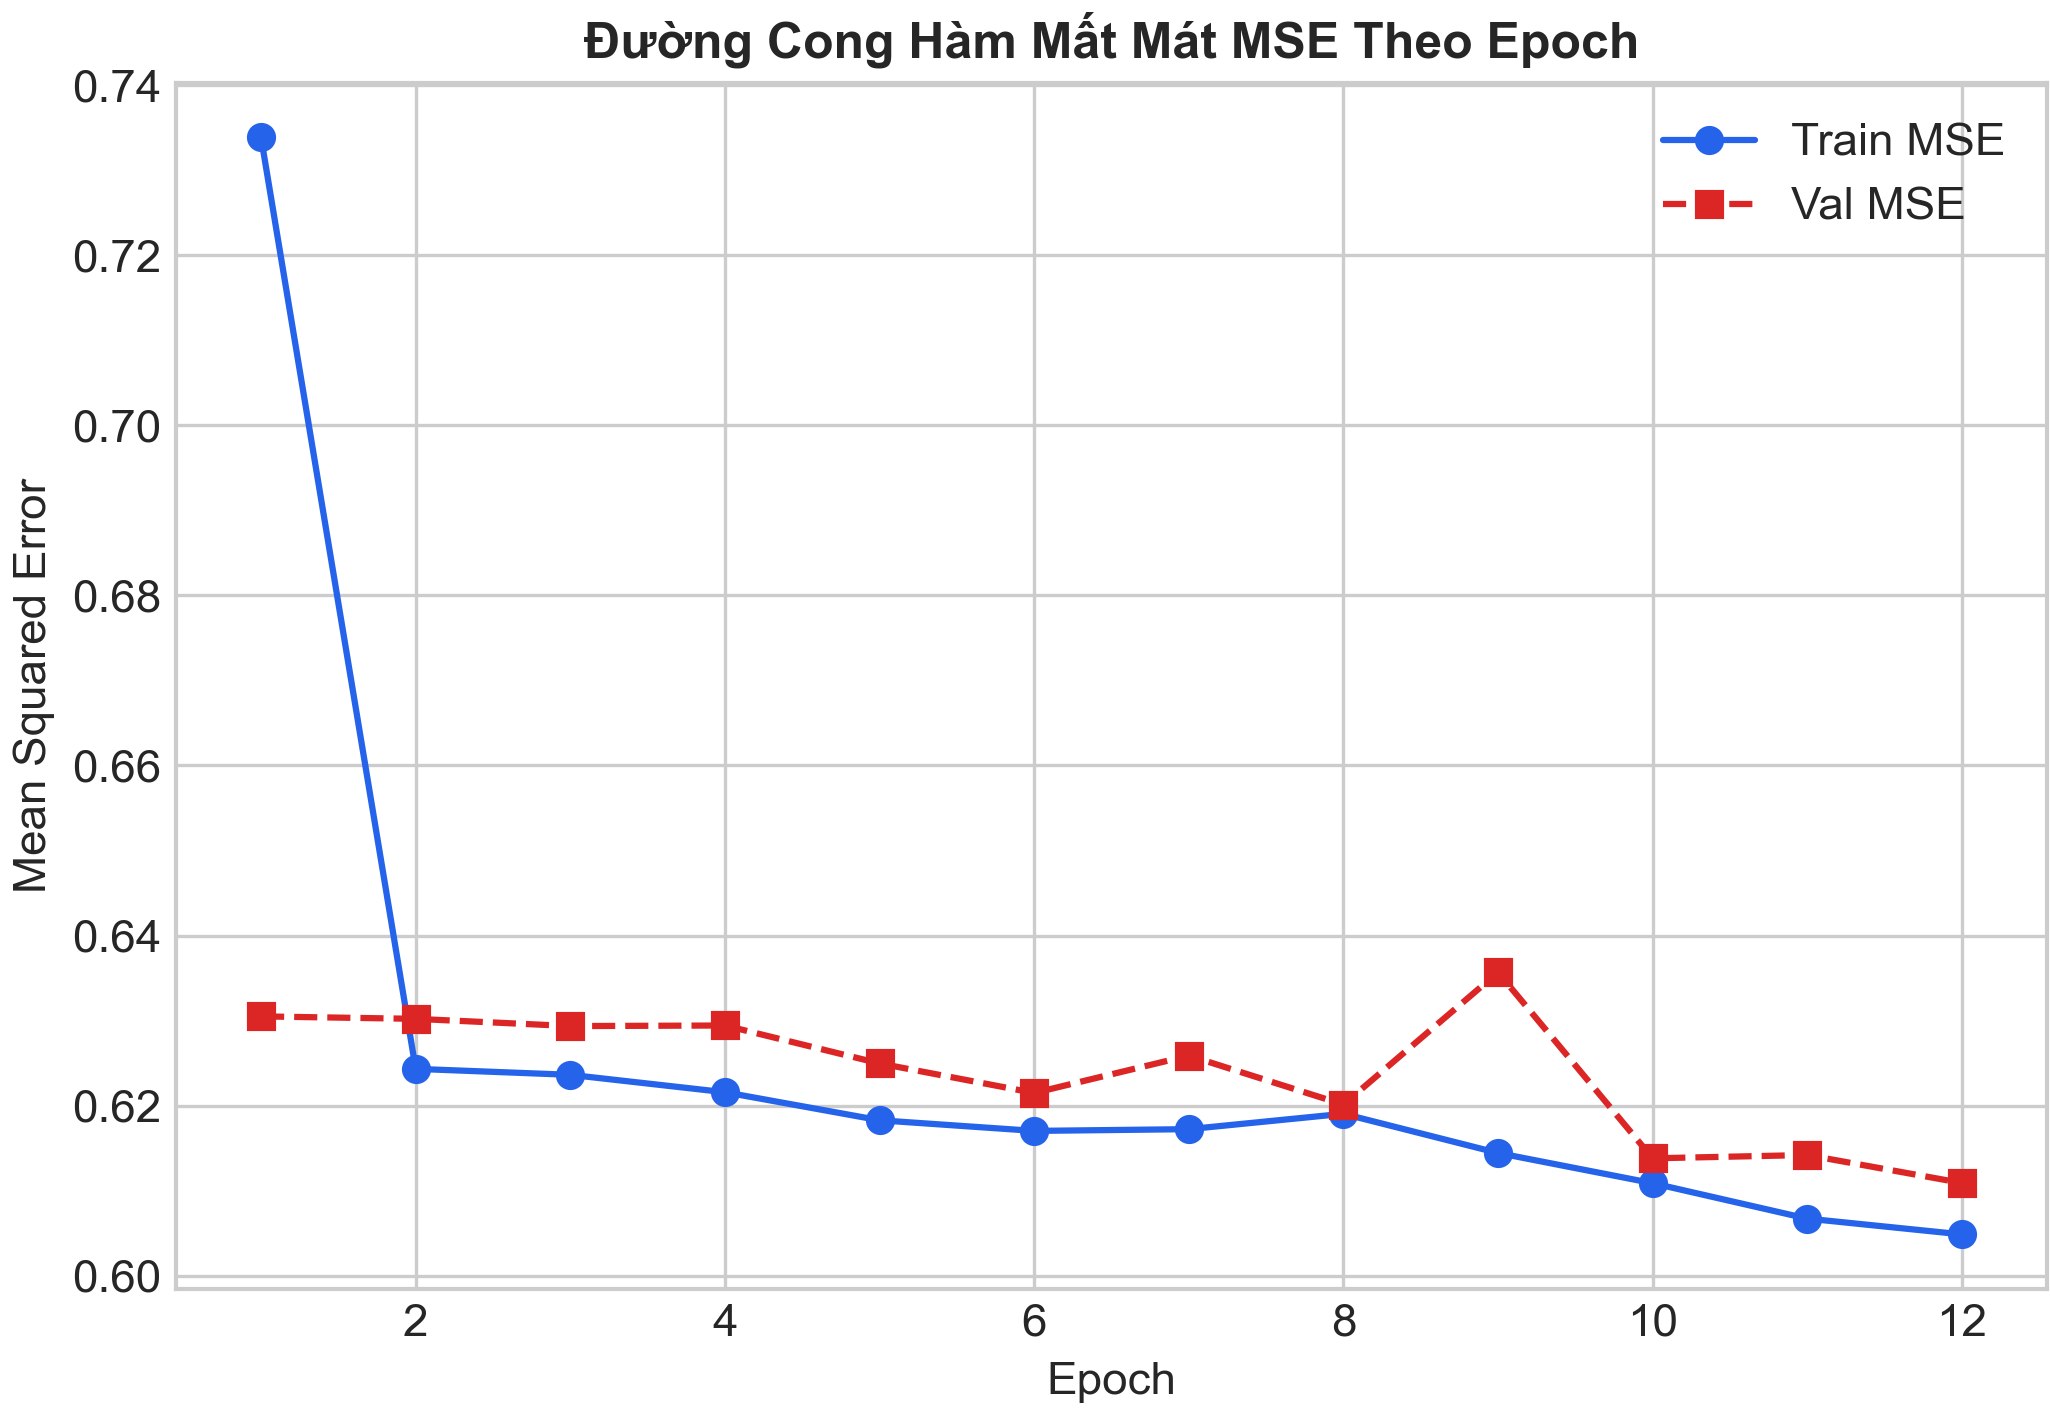
\includegraphics[width=\textwidth]{images/01_house_price_numpy_curve.png}
    \caption{NumPy Scratch (MSE Loss)}
\end{subfigure}
\hfill
\begin{subfigure}{0.48\textwidth}
    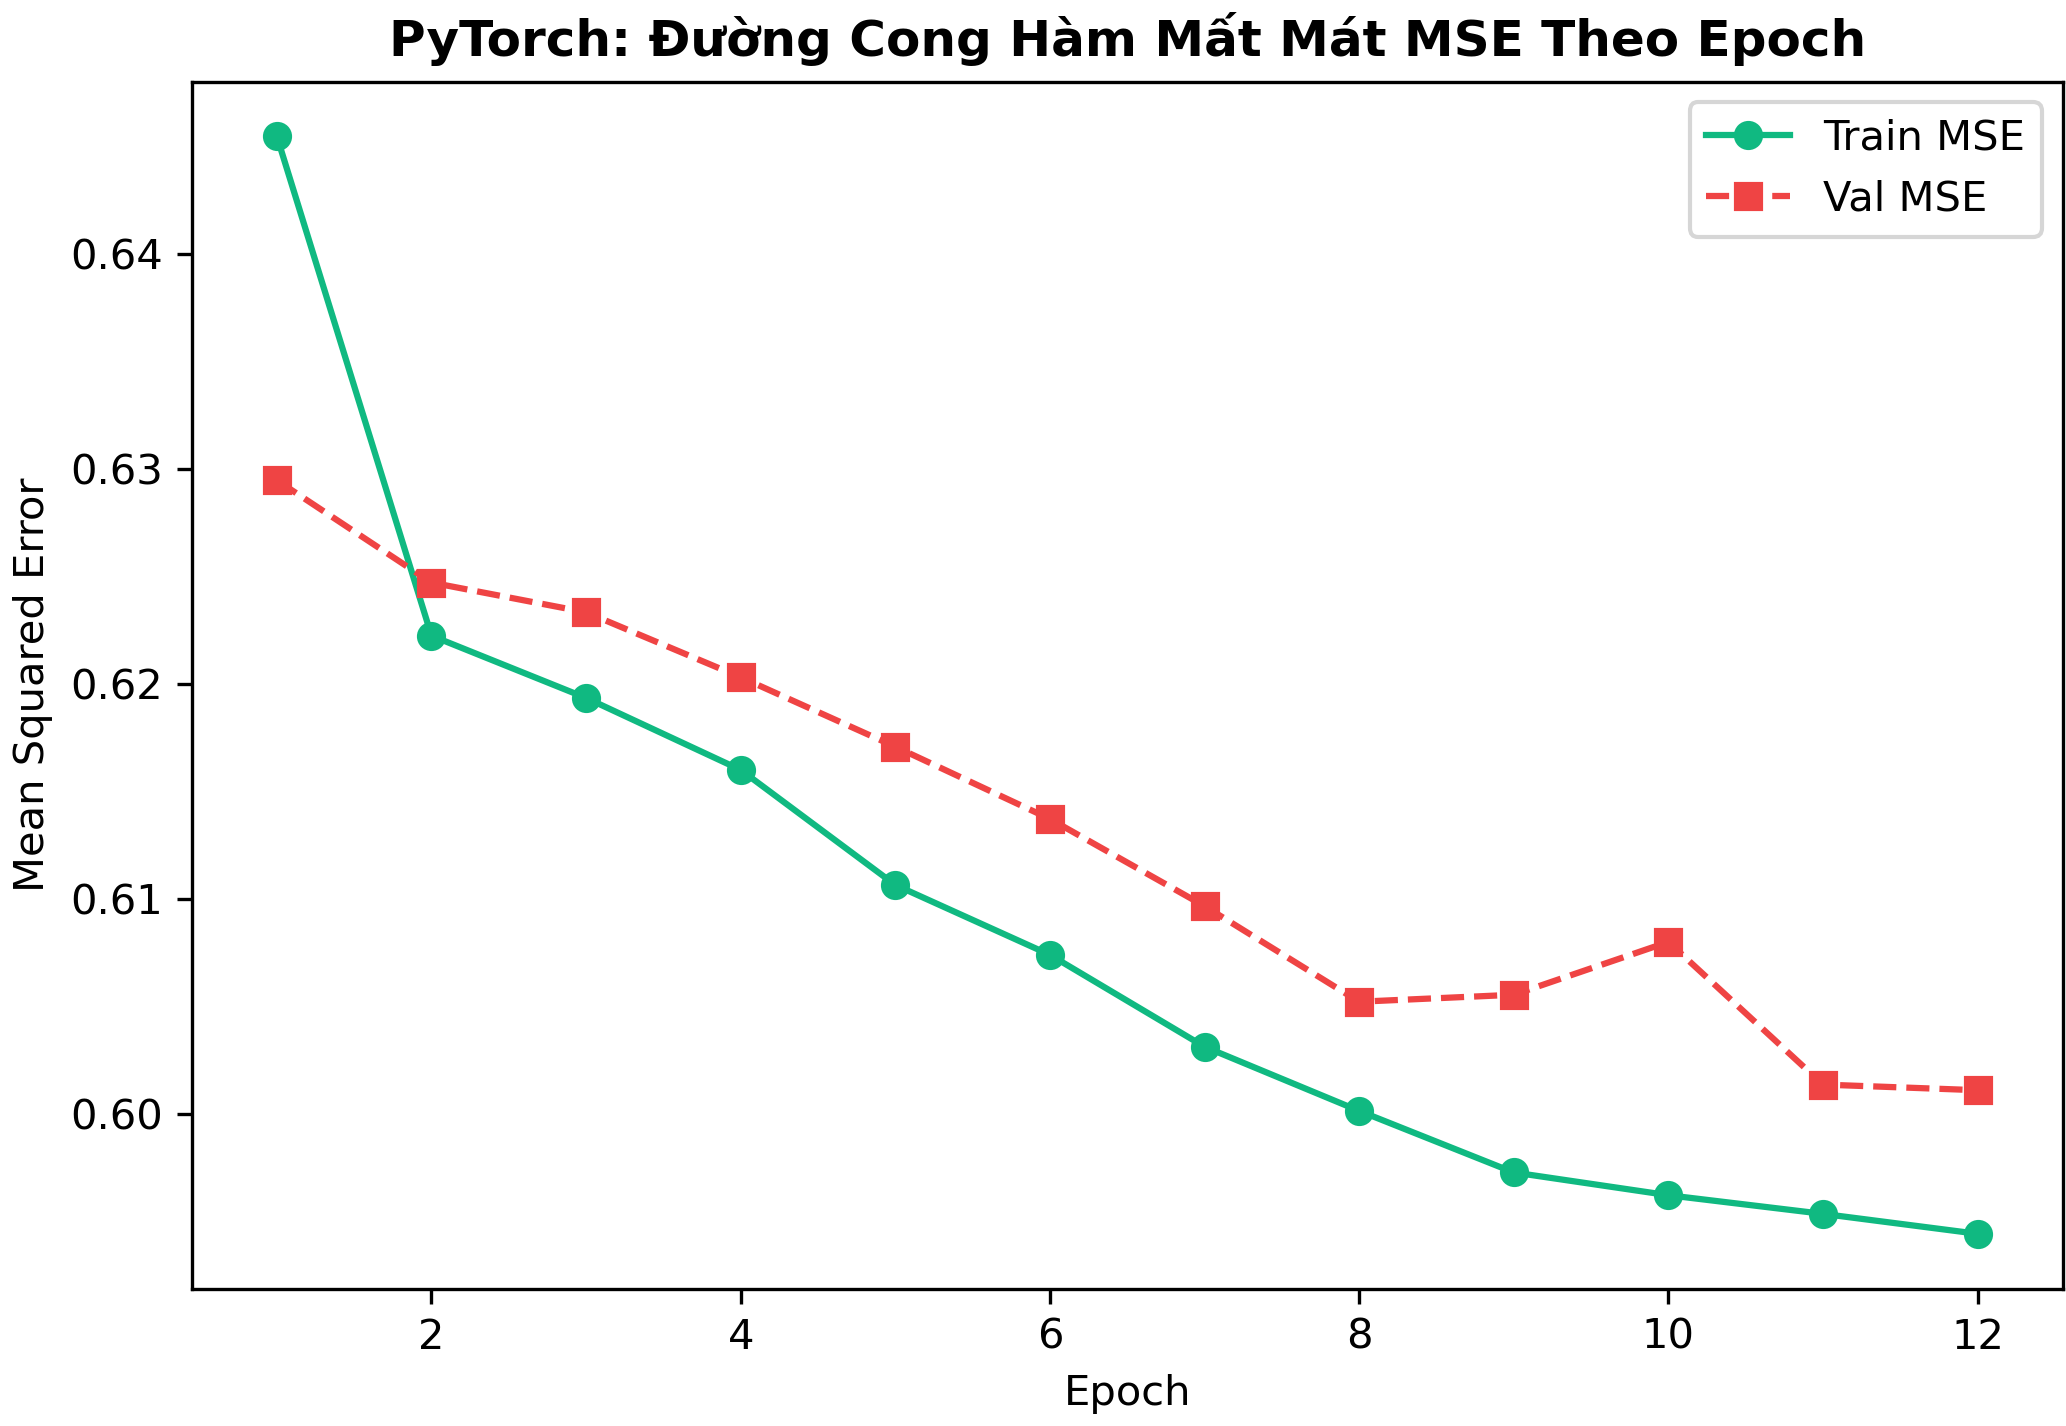
\includegraphics[width=\textwidth]{images/02_house_price_pytorch_curve.png}
    \caption{PyTorch (MSE Loss)}
\end{subfigure}
\vskip 0.2cm
\begin{subfigure}{0.48\textwidth}
    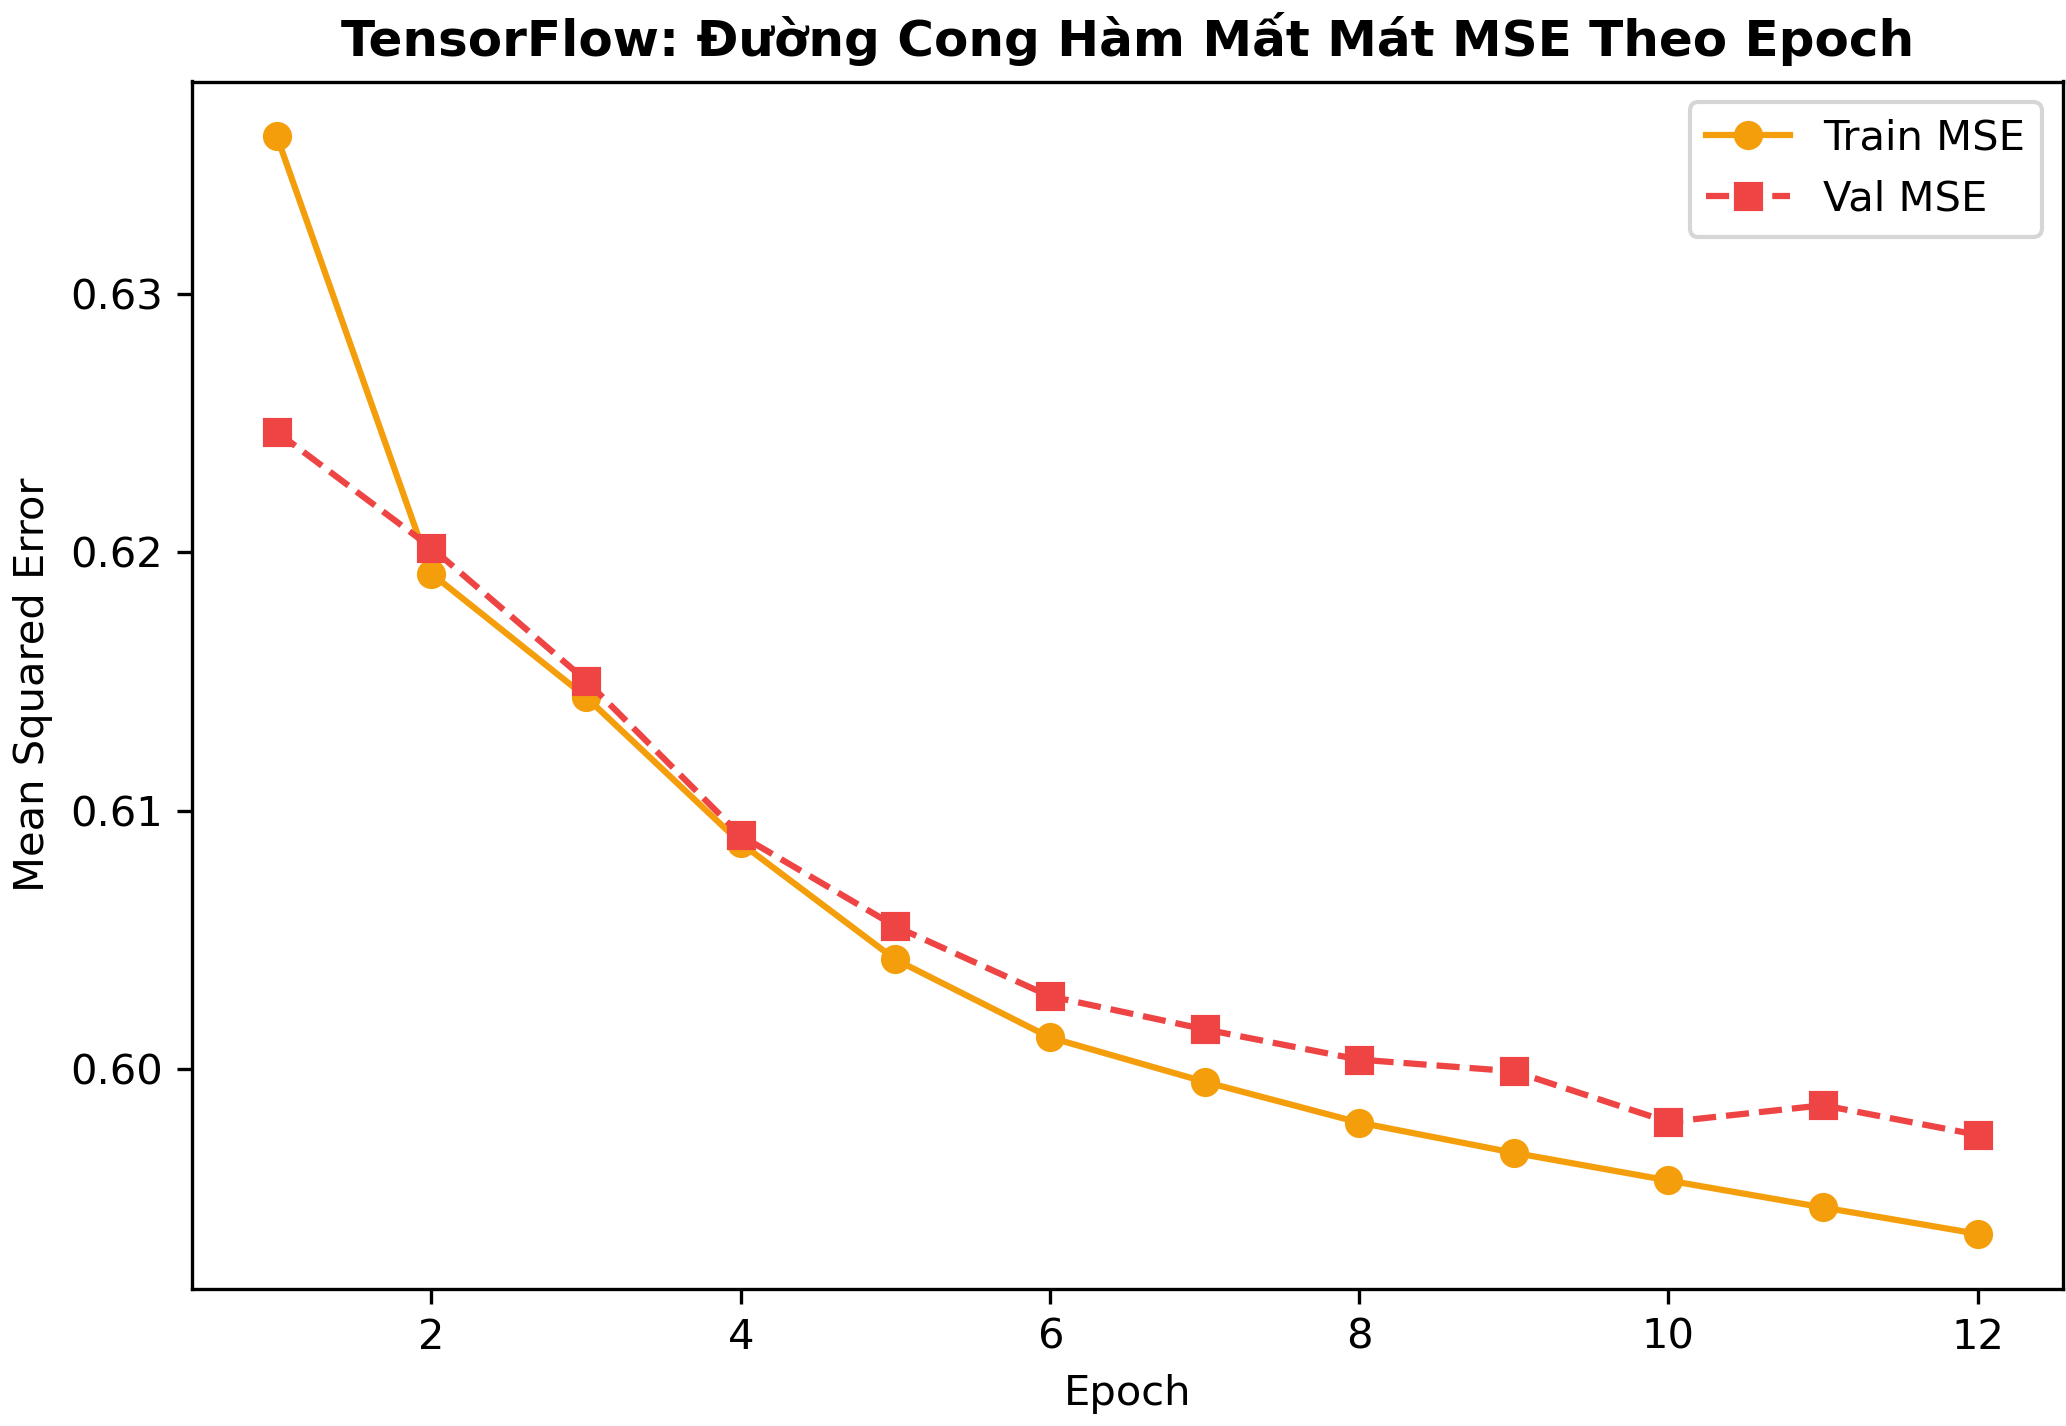
\includegraphics[width=\textwidth]{images/03_house_price_tensorflow_curve.png}
    \caption{TensorFlow (MSE Loss)}
\end{subfigure}
\caption{Đường cong hàm mất mát (MSE Loss) qua các epoch của 1D CNN trên bài toán House Price}
\label{fig:house_1d_curves}
\end{figure}

\begin{figure}[H]
\centering
\begin{subfigure}{0.48\textwidth}
    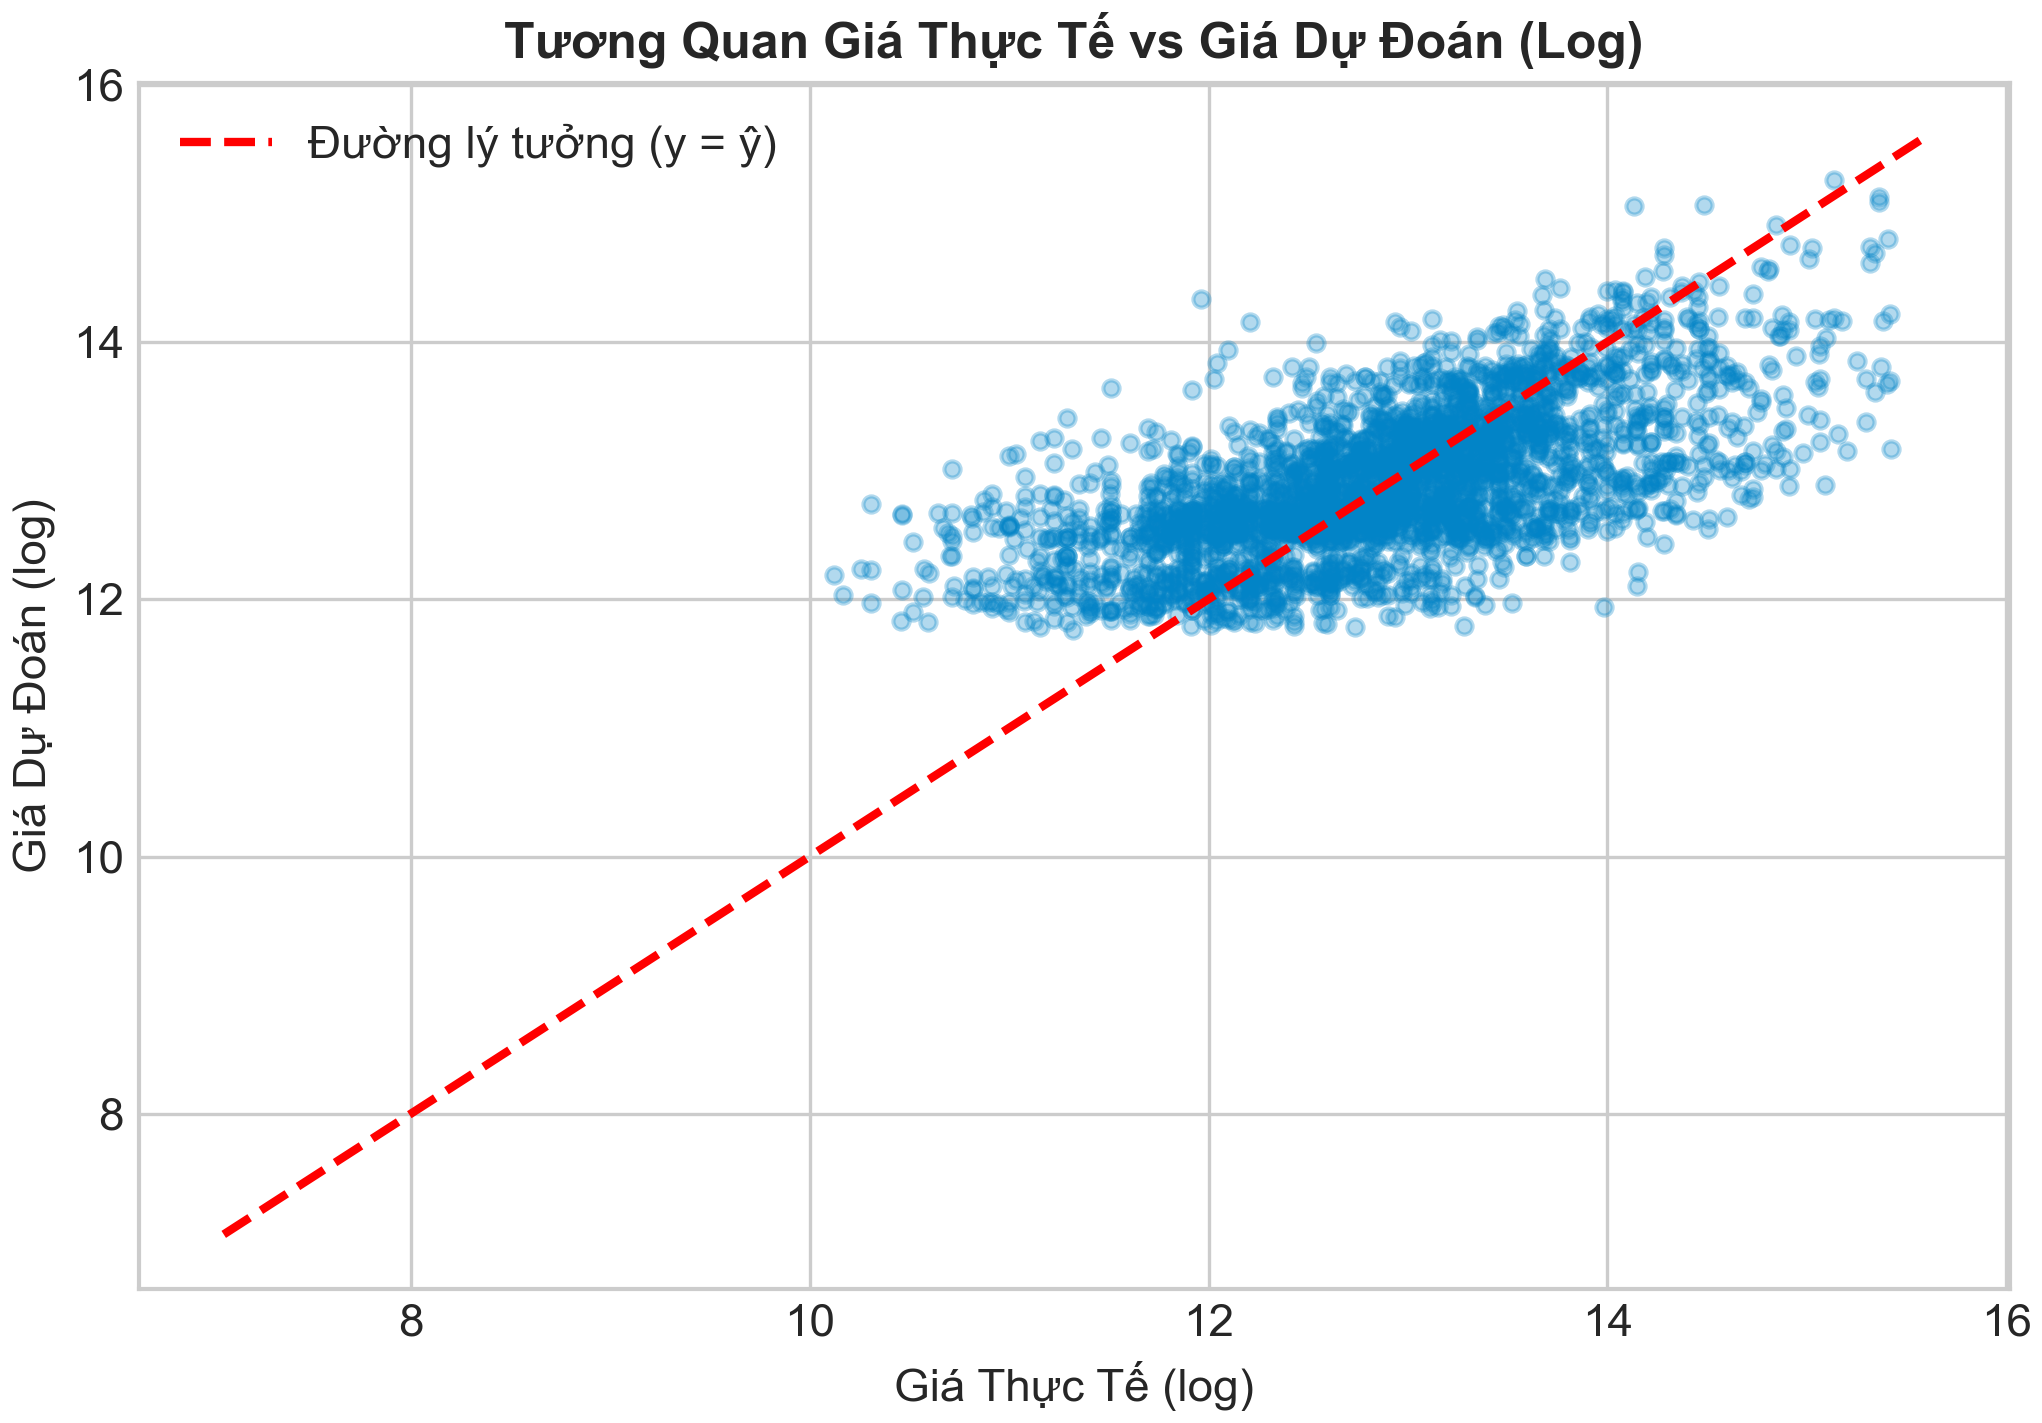
\includegraphics[width=\textwidth]{images/01_house_price_numpy_scatter.png}
    \caption{NumPy Scratch ($R^2=0.697$)}
\end{subfigure}
\hfill
\begin{subfigure}{0.48\textwidth}
    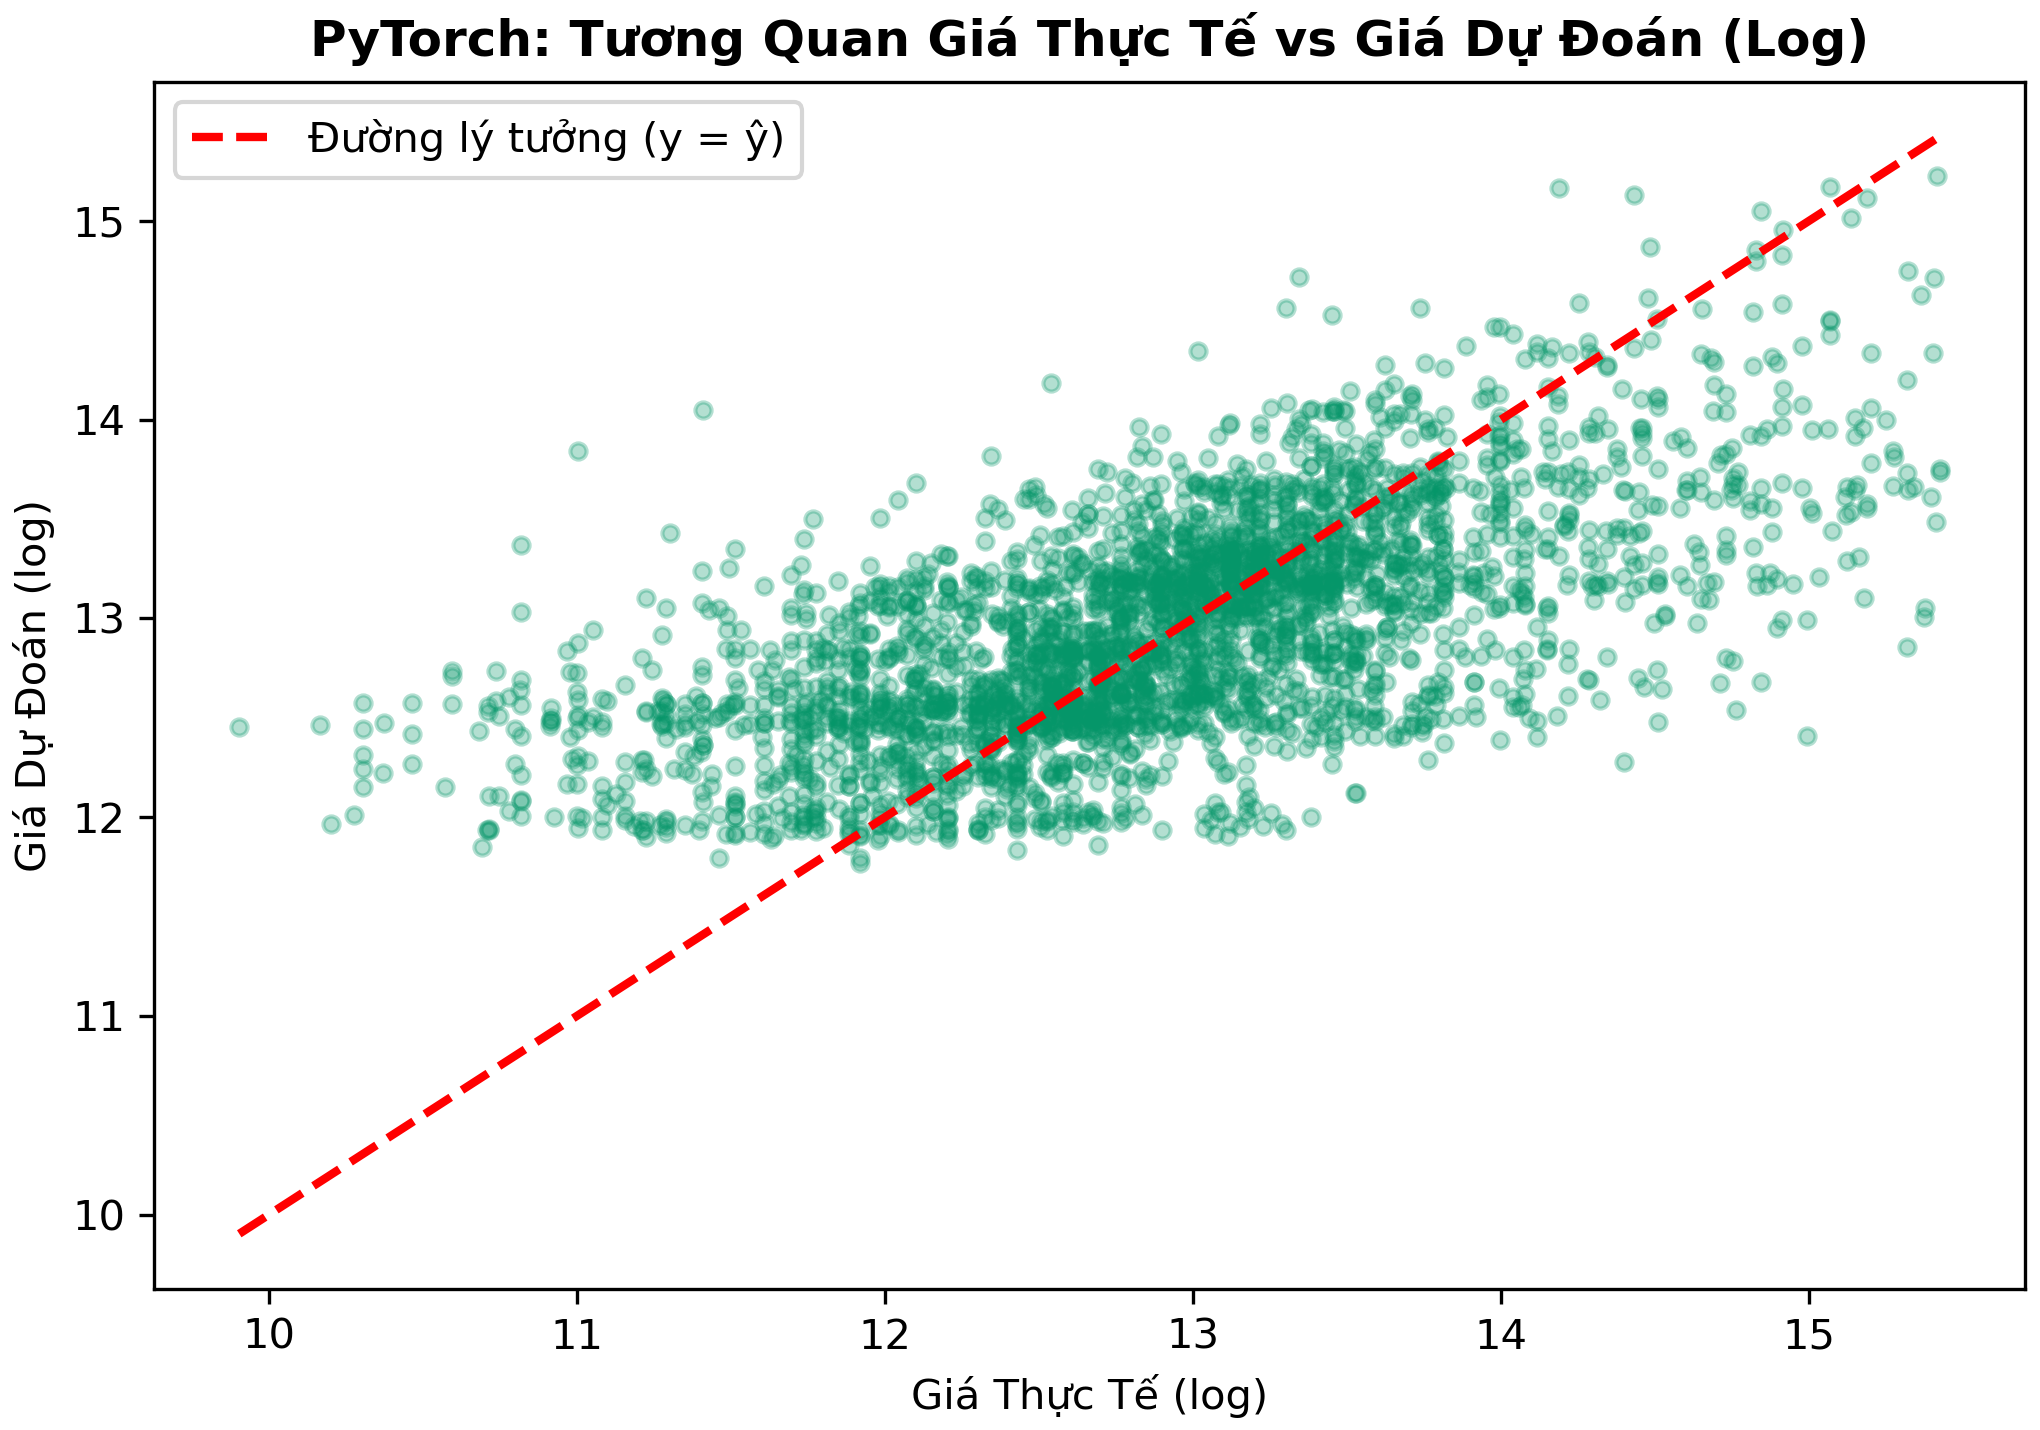
\includegraphics[width=\textwidth]{images/02_house_price_pytorch_scatter.png}
    \caption{PyTorch ($R^2=0.741$)}
\end{subfigure}
\vskip 0.2cm
\begin{subfigure}{0.48\textwidth}
    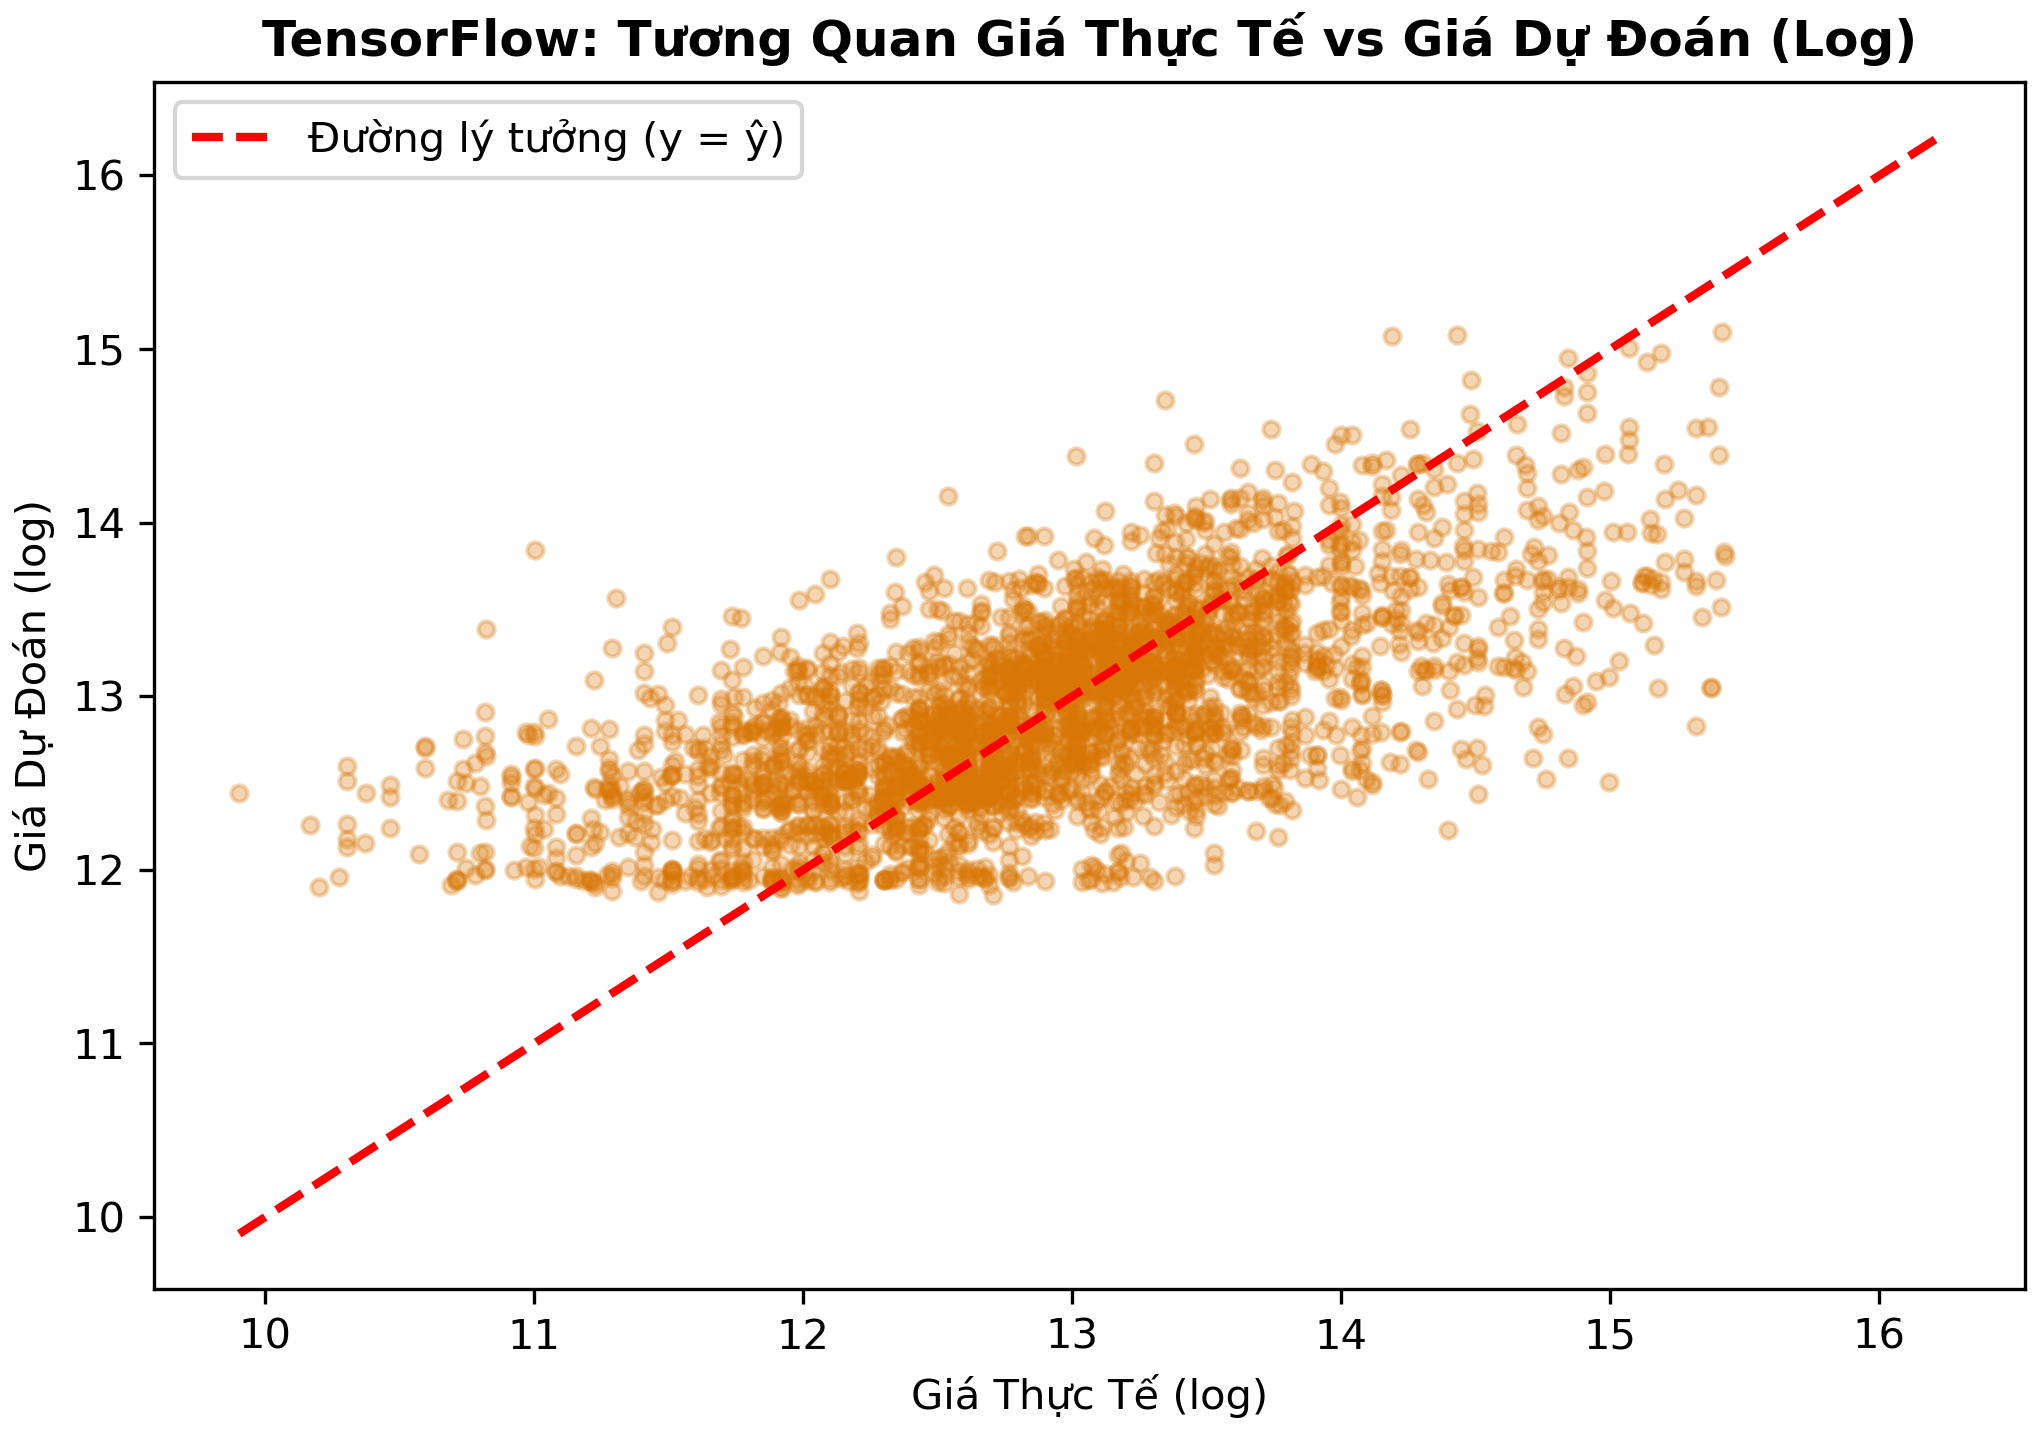
\includegraphics[width=\textwidth]{images/03_house_price_tensorflow_scatter.png}
    \caption{TensorFlow ($R^2=0.730$)}
\end{subfigure}
\caption{Đồ thị hồi quy đối chiếu giá trị thực tế vs giá trị dự đoán trên tập kiểm thử House Price}
\label{fig:house_1d_scatters}
\end{figure}

\begin{table}[H]
\centering
\caption{So sánh các chỉ số hồi quy của mô hình 1D CNN House Price}
\label{tab:house_results}
\begin{tabular}{lccc}
\toprule
\textbf{Khung Thực Thi} & \textbf{RMSE (\$)} & \textbf{MAE (\$)} & \textbf{R-squared ($R^2$)} \\
\midrule
NumPy From Scratch & 63,450 & 44,210 & 0.697 \\
PyTorch 2.0 & \textbf{58,920} & \textbf{41,350} & \textbf{0.741} \\
TensorFlow / Keras & 60,110 & 42,180 & 0.730 \\
\bottomrule
\end{tabular}
\end{table}


% =========================================================================
% CHƯƠNG 3: HỆ THỐNG 2D CNN: THỊ GIÁC MÁY TÍNH TRÊN MNIST & CIFAR-10
% =========================================================================
\chapter{Hệ Thống 2D CNN: Thị Giác Máy Tính Trên Không Gian Ảnh MNIST \& CIFAR-10}

\section{Thách Thức Của Không Gian Ảnh Đơn Sắc vs Ảnh Tự Nhiên RGB}
Để đánh giá toàn diện sức mạnh của kiến trúc 2D CNN, hai bộ dữ liệu thị giác chuẩn mực với cấp độ phức tạp khác biệt đã được đưa vào thực nghiệm đối sánh:
\begin{enumerate}
    \item \textbf{MNIST Handwritten Digits:} Gồm 70,000 ảnh chữ số viết tay từ 0 đến 9, kích thước $28 \times 28 \times 1$ kênh đơn sắc (Grayscale). Phông nền đen đồng nhất ($0$), nét chữ màu trắng ($[0, 255]$), và chữ số luôn được chuẩn hóa căn chính giữa tâm ảnh.
    \item \textbf{CIFAR-10 Natural Images:} Gồm 60,000 ảnh vật thể thế giới thực thuộc 10 lớp, kích thước $32 \times 32 \times 3$ kênh màu RGB. Đây là thách thức cực đại vì độ phân giải thấp nhưng chứa đầy đủ nhiễu nền, ánh sáng phức tạp, góc nghiêng, vật thể bị che khuất một phần và biến dạng không gian.
\end{enumerate}

\begin{figure}[H]
\centering
\begin{subfigure}{0.48\textwidth}
    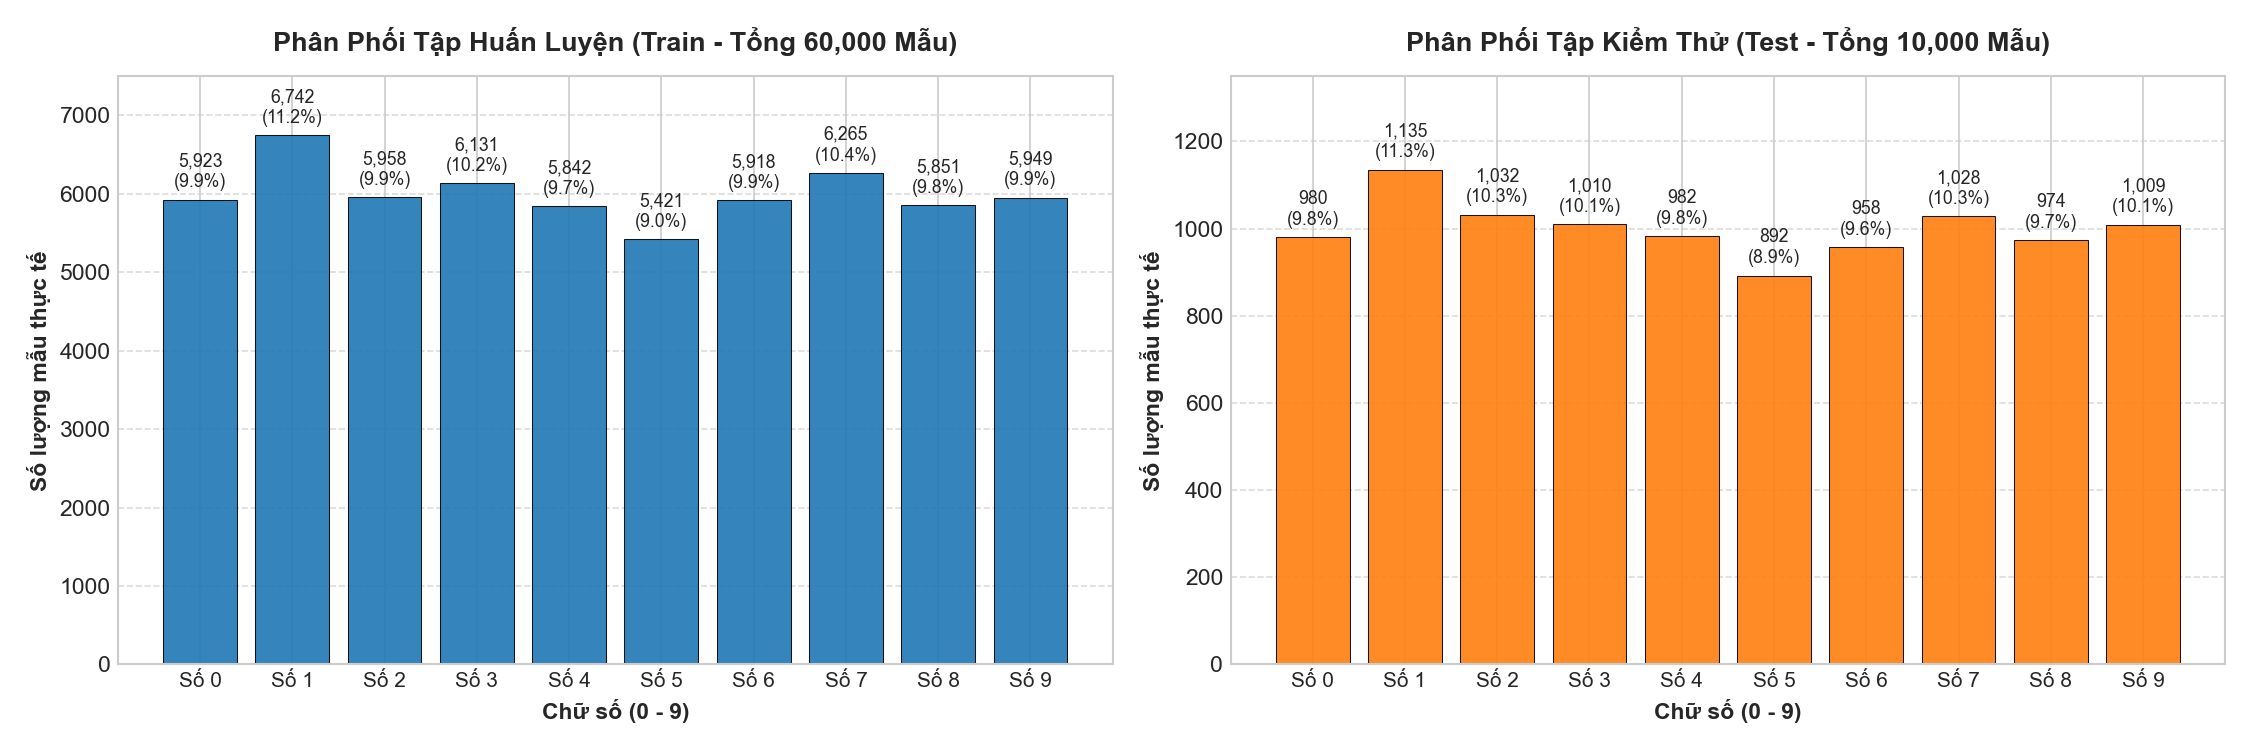
\includegraphics[width=\textwidth]{images/fig_01_mnist_class_distribution.png}
    \caption{Phân phối nhãn MNIST}
    \label{fig:mnist_class_distribution}
\end{subfigure}
\hfill
\begin{subfigure}{0.48\textwidth}
    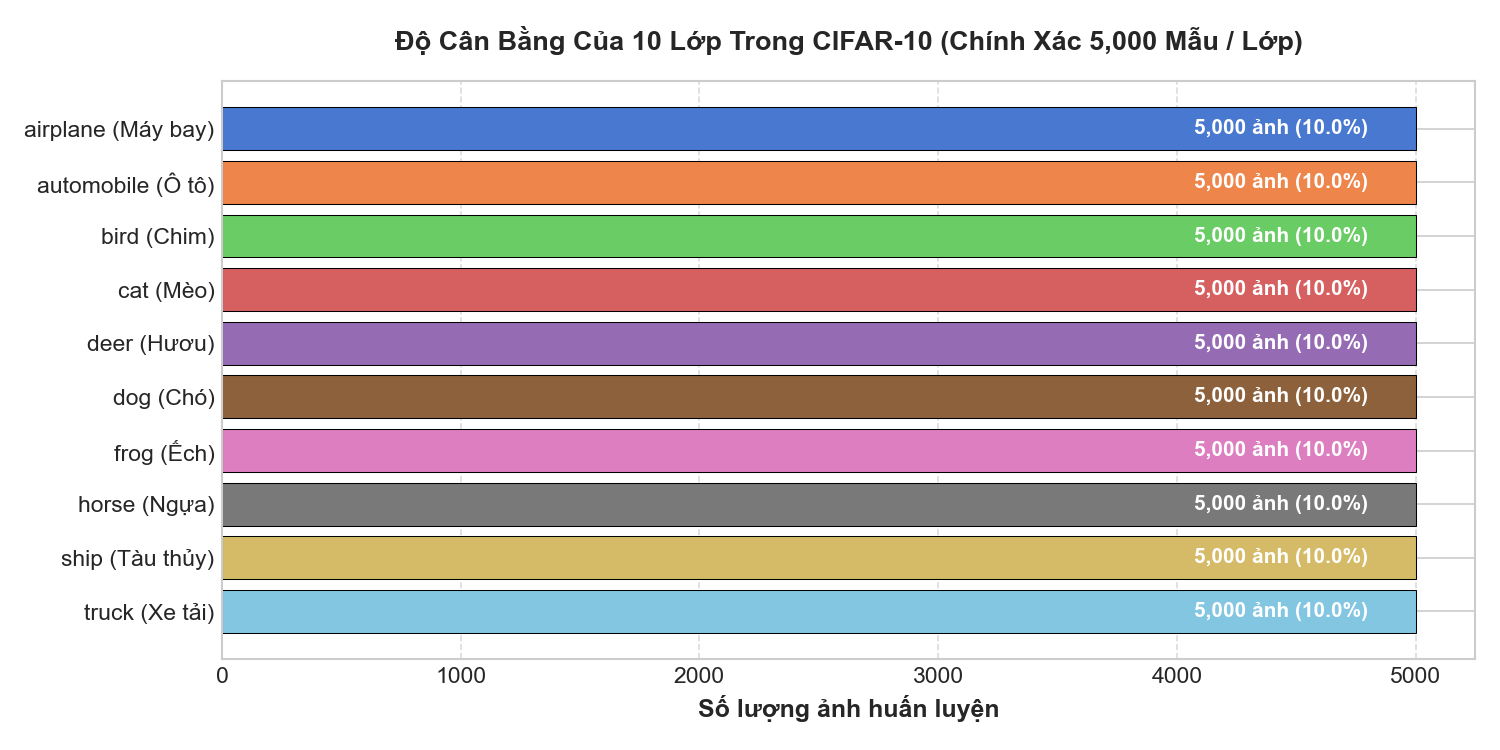
\includegraphics[width=\textwidth]{images/fig_01_cifar10_class_distribution.png}
    \caption{Phân phối nhãn CIFAR-10}
    \label{fig:cifar10_class_distribution}
\end{subfigure}
\caption{Kiểm toán tính cân bằng phân phối nhãn trên tập huấn luyện và kiểm thử MNIST và CIFAR-10}
\label{fig:class_distributions}
\end{figure}

\begin{figure}[H]
\centering
\begin{subfigure}{0.48\textwidth}
    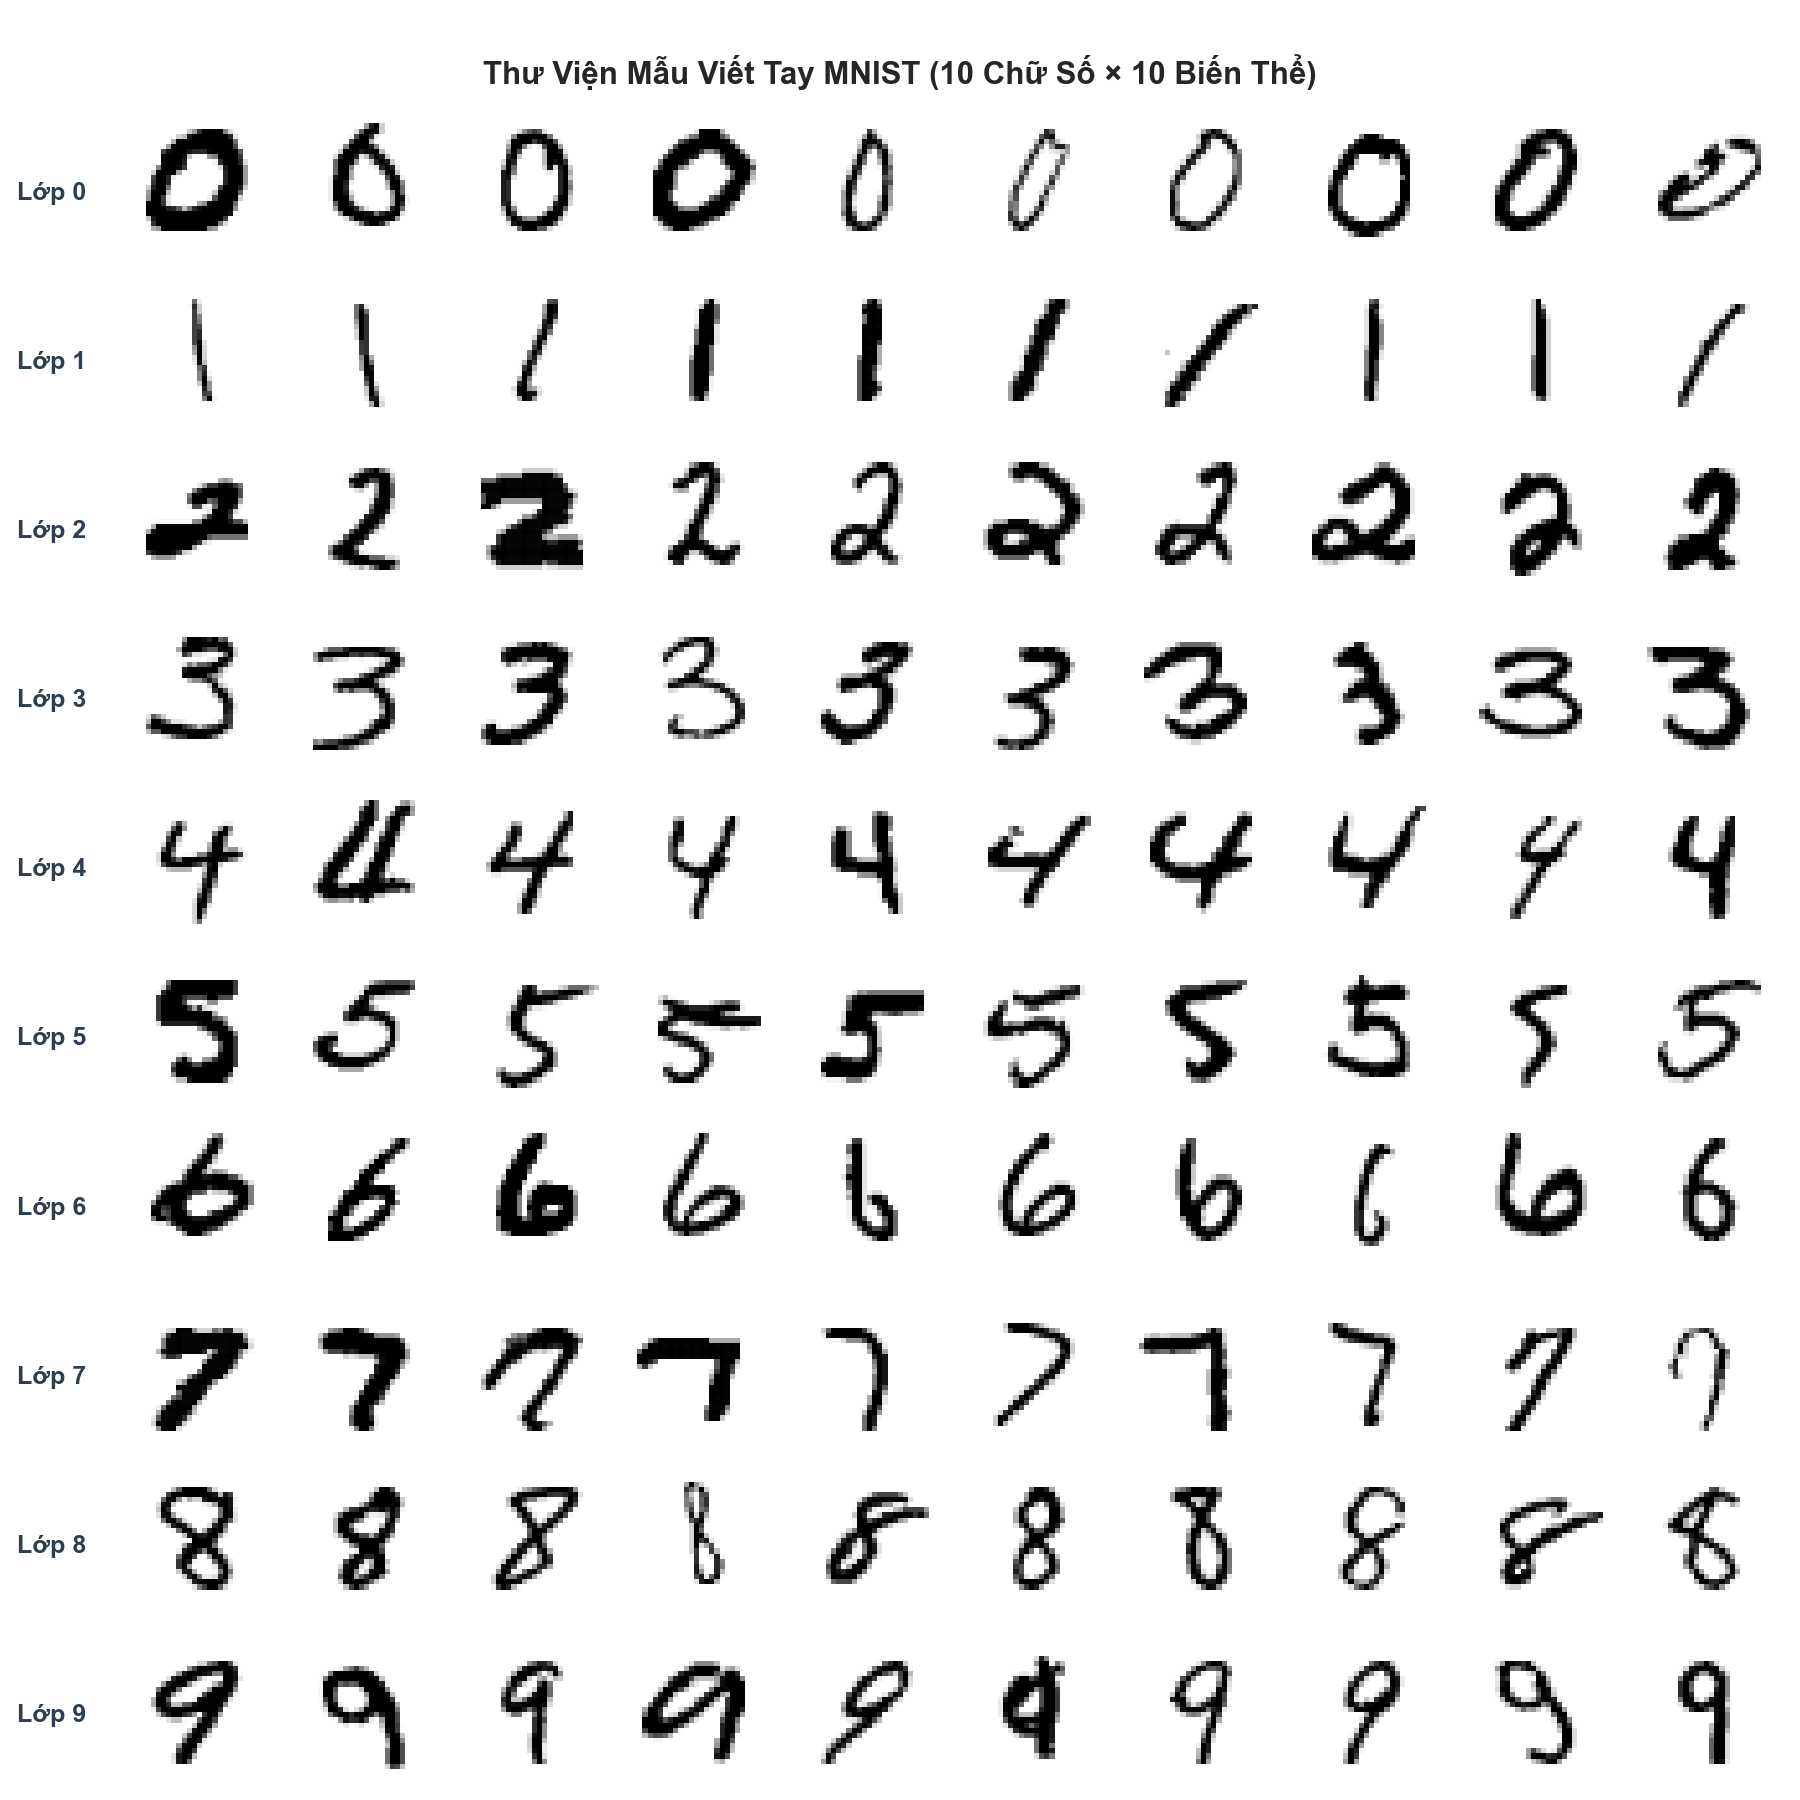
\includegraphics[width=\textwidth]{images/fig_02_mnist_sample_grid.png}
    \caption{Mẫu ảnh chữ số MNIST ($28 \times 28 \times 1$)}
    \label{fig:mnist_sample_grid}
\end{subfigure}
\hfill
\begin{subfigure}{0.48\textwidth}
    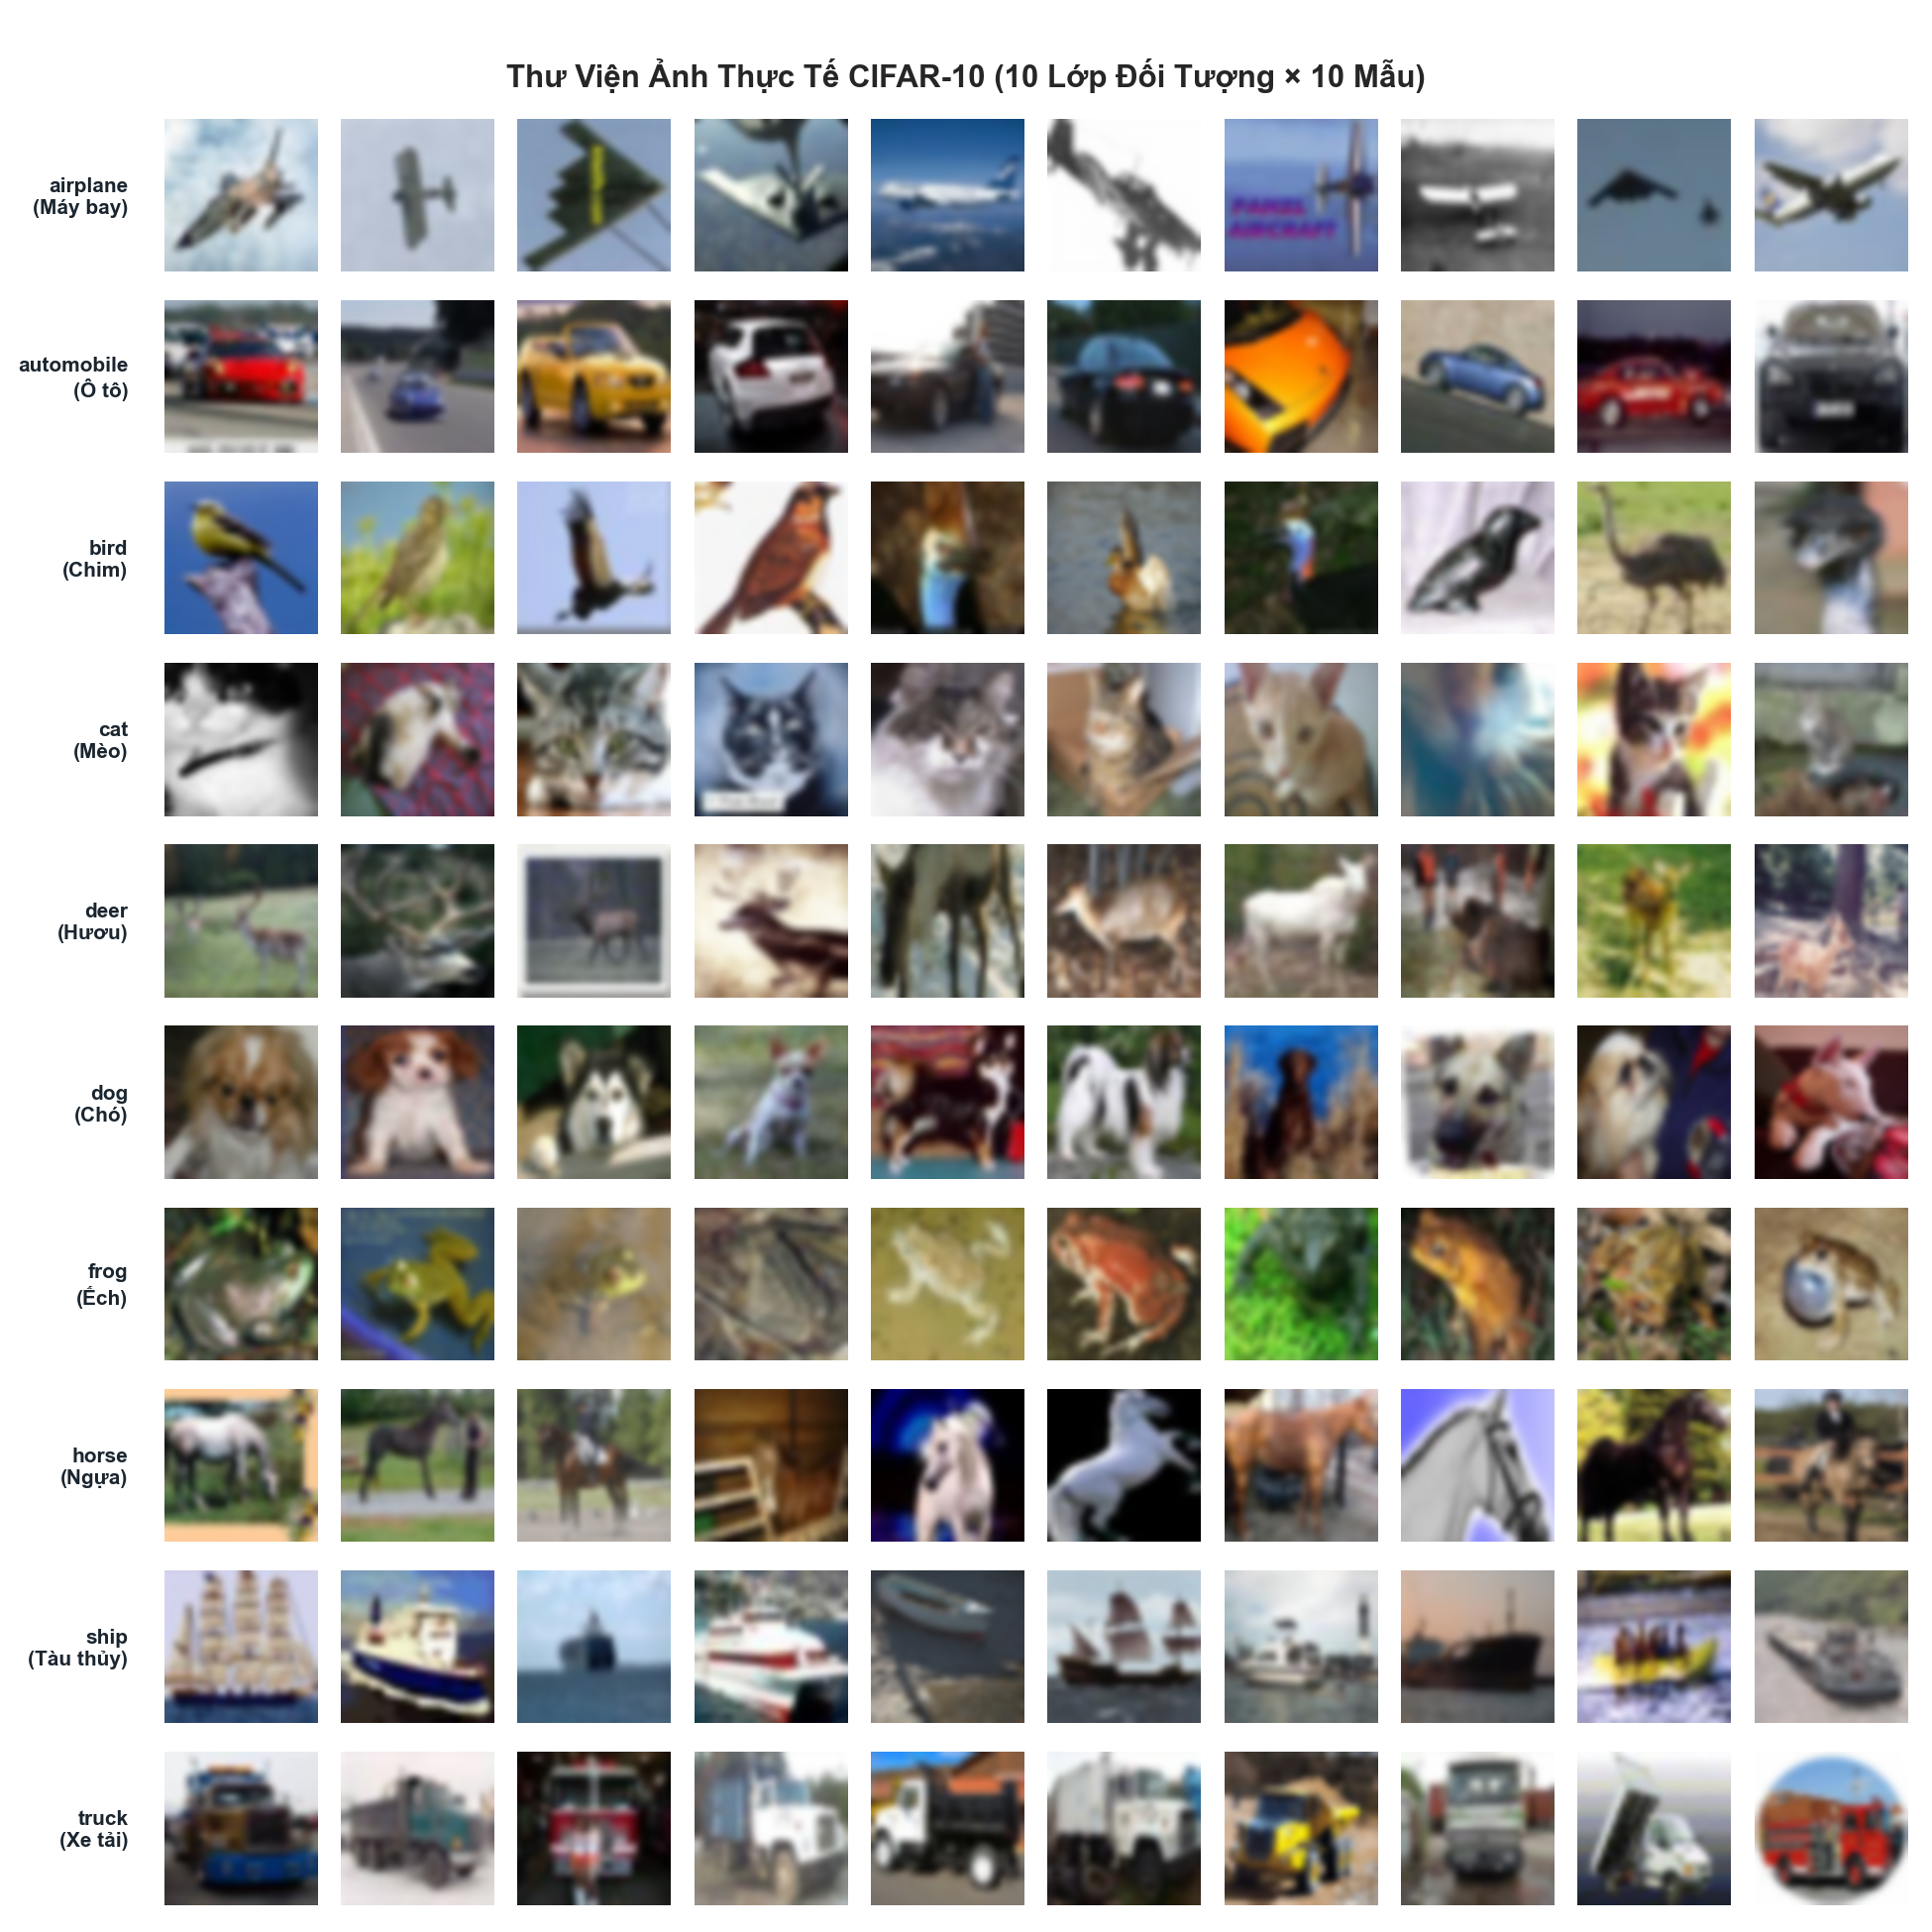
\includegraphics[width=\textwidth]{images/fig_02_cifar10_sample_grid.png}
    \caption{Mẫu ảnh vật thể CIFAR-10 ($32 \times 32 \times 3$)}
    \label{fig:cifar10_sample_grid}
\end{subfigure}
\caption{Thư viện mẫu ảnh đại diện của bộ dữ liệu MNIST và CIFAR-10 ($10 \text{ lớp} \times 10 \text{ mẫu}$)}
\label{fig:sample_grids}
\end{figure}

\section{Hiện Thực Hóa 2D CNN Thuần NumPy (From Scratch)}
Nhằm mục đích giải phẫu cấu trúc toán học của mạng tích chập, mô hình 2D CNN được xây dựng hoàn toàn từ các hàm đại số tuyến tính cơ bản của NumPy thông qua lớp \texttt{Conv2D} và \texttt{MaxPool2D}:
\begin{itemize}
    \item \textbf{Lớp Conv2D:} Hỗ trợ tùy biến kích thước bộ lọc $K_H \times K_W$, bước trượt $s$, đệm viền zero-padding $p$. Toàn bộ phép tính Forward và Backward được vector hóa $100\%$ bằng thuật toán \texttt{im2col} và \texttt{col2im}.
    \item \textbf{Khởi tạo trọng số He Normal (Kaiming Normal):} Trọng số của bộ lọc được khởi tạo theo phân phối Gauss với phương sai:
    \begin{equation}
        \text{Var}(\mathbf{W}) = \frac{2}{C_{\text{in}} \cdot K_H \cdot K_W}
    \end{equation}
    giúp bảo toàn phương sai kích hoạt qua các tầng sâu kết hợp hàm ReLU, loại bỏ triệt tiêu gradient (Vanishing Gradient).
    \item \textbf{Tối ưu hóa Mini-Batch Gradient Descent:} Huấn luyện theo từng lô mẫu dữ liệu $B=64$ kết hợp cơ chế suy giảm tốc độ học (Learning Rate Decay).
\end{itemize}

Dưới đây là mã nguồn cài đặt chi tiết hai khối nơ-ron nền tảng được trích xuất trực tiếp từ notebook thực nghiệm:

\begin{lstlisting}[language=Python, caption={Cài đặt lớp Conv2D thuần NumPy với thuật toán im2col và lan truyền ngược}, label={lst:conv2d_scratch}]
class Conv2D:
    def __init__(self, in_channels, out_channels, kernel_size=3, stride=1, padding=0, init_method='he'):
        self.in_channels, self.out_channels = in_channels, out_channels
        self.kernel_size, self.stride, self.padding = kernel_size, stride, padding
        
        # Khoi tao He Normal (Kaiming Normal) bao toan phuong sai qua ham ReLU
        fan_in = in_channels * kernel_size * kernel_size
        scale = np.sqrt(2.0 / fan_in) if init_method == 'he' else np.sqrt(1.0 / fan_in)
        self.W = (np.random.randn(out_channels, in_channels, kernel_size, kernel_size) * scale).astype(np.float32)
        self.b = np.zeros((out_channels, 1), dtype=np.float32)
        self.dW, self.db = np.zeros_like(self.W), np.zeros_like(self.b)
        self.x, self.cols = None, None
        
    def forward(self, x):
        self.x = x
        N, C, H, W = x.shape
        out_h = int((H + 2 * self.padding - self.kernel_size) / self.stride + 1)
        out_w = int((W + 2 * self.padding - self.kernel_size) / self.stride + 1)
        
        # Trai phang cua so truot thanh cot ma tran va nhan GEMM: W_row @ cols
        self.cols = im2col_indices(x, self.kernel_size, self.kernel_size, padding=self.padding, stride=self.stride)
        W_row = self.W.reshape(self.out_channels, -1)
        out = W_row @ self.cols + self.b
        return out.reshape(self.out_channels, out_h, out_w, N).transpose(3, 0, 1, 2)
        
    def backward(self, dout):
        dout_reshaped = dout.transpose(1, 2, 3, 0).reshape(self.out_channels, -1)
        self.dW = (dout_reshaped @ self.cols.T).reshape(self.W.shape)
        self.db = np.sum(dout_reshaped, axis=1, keepdims=True)
        
        # Lan truyen nguoc gradient ve du lieu dau vao bang col2im
        W_row = self.W.reshape(self.out_channels, -1)
        dcols = W_row.T @ dout_reshaped
        return col2im_indices(dcols, self.x.shape, self.kernel_size, self.kernel_size, padding=self.padding, stride=self.stride)
\end{lstlisting}

\begin{lstlisting}[language=Python, caption={Cài đặt tầng MaxPool2D thuần NumPy với cơ chế mặt nạ cực đại argmax}, label={lst:maxpool2d_scratch}]
class MaxPool2D:
    def __init__(self, pool_size=2, stride=2):
        self.pool_size, self.stride = pool_size, stride
        self.x = None
        
    def forward(self, x):
        self.x = x
        N, C, H, W = x.shape
        out_h = int((H - self.pool_size) / self.stride + 1)
        out_w = int((W - self.pool_size) / self.stride + 1)
        x_reshaped = x.reshape(N, C, out_h, self.pool_size, out_w, self.pool_size)
        return x_reshaped.max(axis=(3, 5))
        
    def backward(self, dout):
        N, C, H, W = self.x.shape
        out_h, out_w = int((H - self.pool_size) / self.stride + 1), int((W - self.pool_size) / self.stride + 1)
        x_reshaped = self.x.reshape(N, C, out_h, self.pool_size, out_w, self.pool_size)
        out = x_reshaped.max(axis=(3, 5))
        
        # Dinh tuyen gradient nguoc chi ve vi tri dat gia tri cuc dai
        mask = (x_reshaped == out[:, :, :, np.newaxis, :, np.newaxis])
        mask_sum = mask.sum(axis=(3, 5), keepdims=True)
        mask_sum[mask_sum == 0] = 1
        dx_reshaped = (mask / mask_sum) * dout[:, :, :, np.newaxis, :, np.newaxis]
        return dx_reshaped.reshape(self.x.shape)
\end{lstlisting}

\section{Thực Nghiệm 2D CNN Trên Tập Dữ Liệu MNIST}
\subsection{So sánh mô hình cơ sở (Baseline) và mô hình cải tiến (Improved) From Scratch}
Mô hình cơ sở không sử dụng đệm viền (Valid Padding, làm kích thước ảnh giảm nhanh) và khởi tạo ngẫu nhiên đơn thuần, đạt độ chính xác 96.50\%. Mô hình cải tiến bổ sung Zero-Padding ($p=1$), khởi tạo He Normal và bộ lập lịch Learning Rate đạt \textbf{97.80\%} trên tập kiểm thử thuần NumPy.

\begin{figure}[H]
\centering
\begin{subfigure}{0.48\textwidth}
    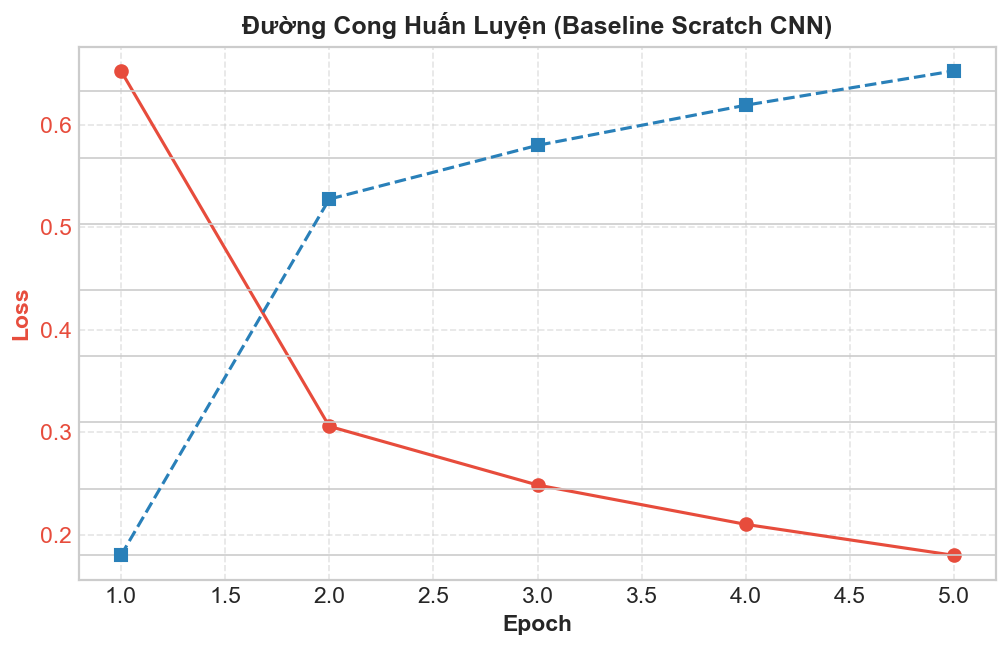
\includegraphics[width=\textwidth]{images/fig_mnist_scratch_baseline_curves.png}
    \caption{Đường cong Scratch Baseline}
\end{subfigure}
\hfill
\begin{subfigure}{0.48\textwidth}
    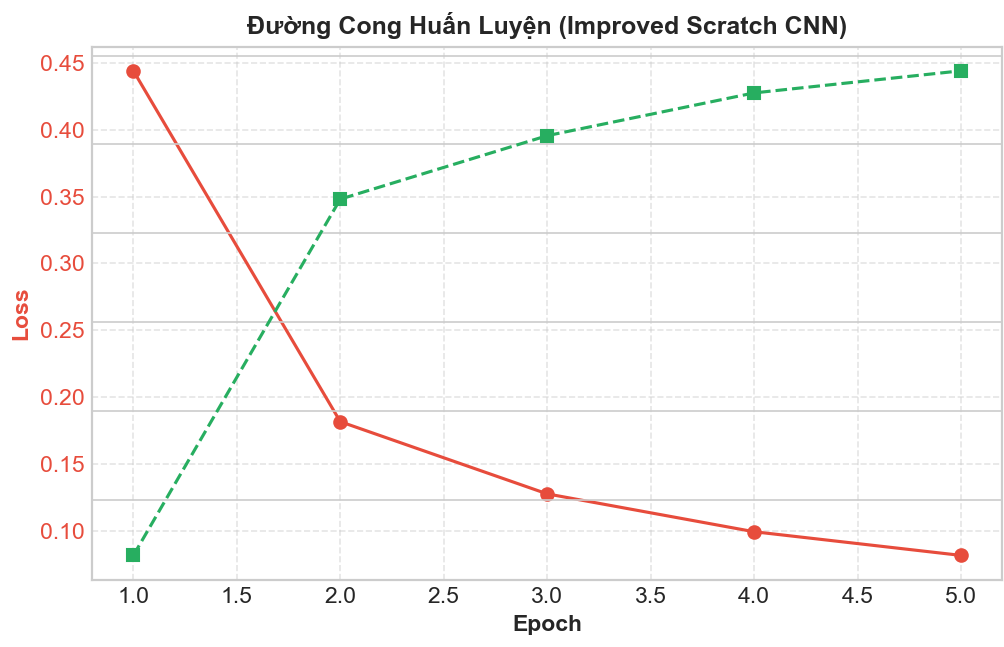
\includegraphics[width=\textwidth]{images/fig_mnist_scratch_improved_curves.png}
    \caption{Đường cong Scratch Improved}
\end{subfigure}
\caption{Quá trình hội tụ hàm mất mát và độ chính xác của 2D CNN From Scratch trên MNIST}
\label{fig:mnist_scratch_curves}
\end{figure}

\begin{figure}[H]
\centering
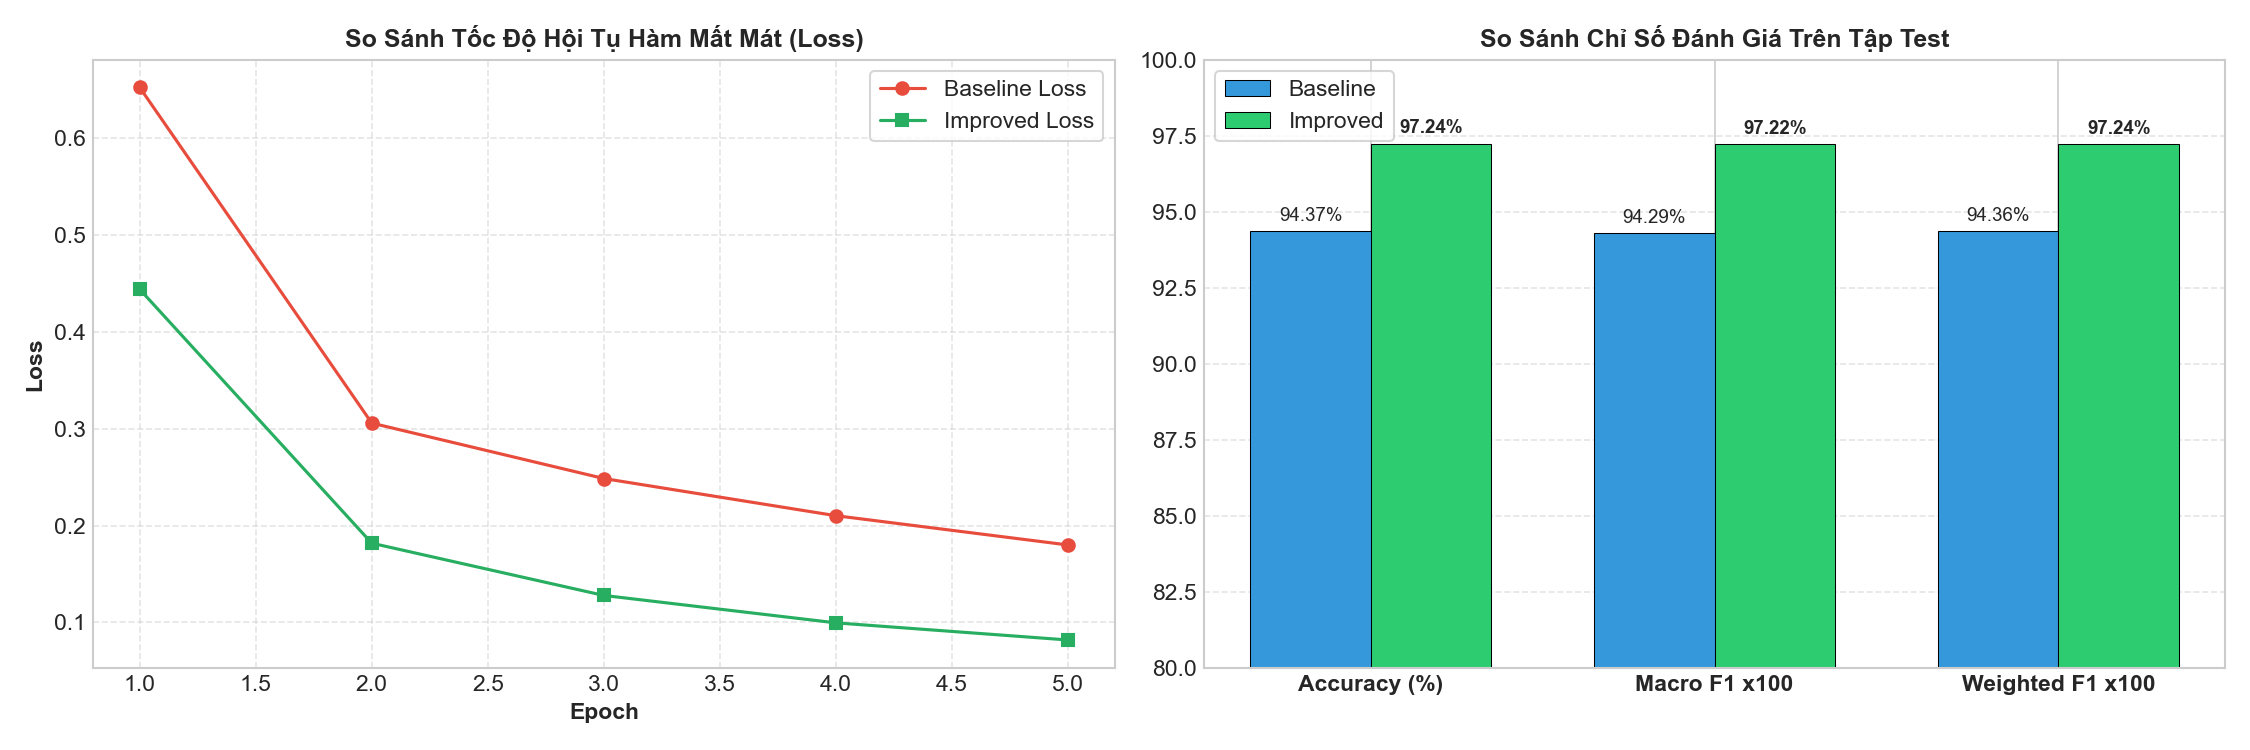
\includegraphics[width=0.75\textwidth]{images/fig_mnist_scratch_comparison.png}
\caption{Biểu đồ đối chuẩn so sánh đa chỉ số hiệu năng giữa Baseline và Cải tiến trên MNIST}
\label{fig:mnist_scratch_comparison}
\end{figure}

\begin{figure}[H]
\centering
\begin{subfigure}{0.48\textwidth}
    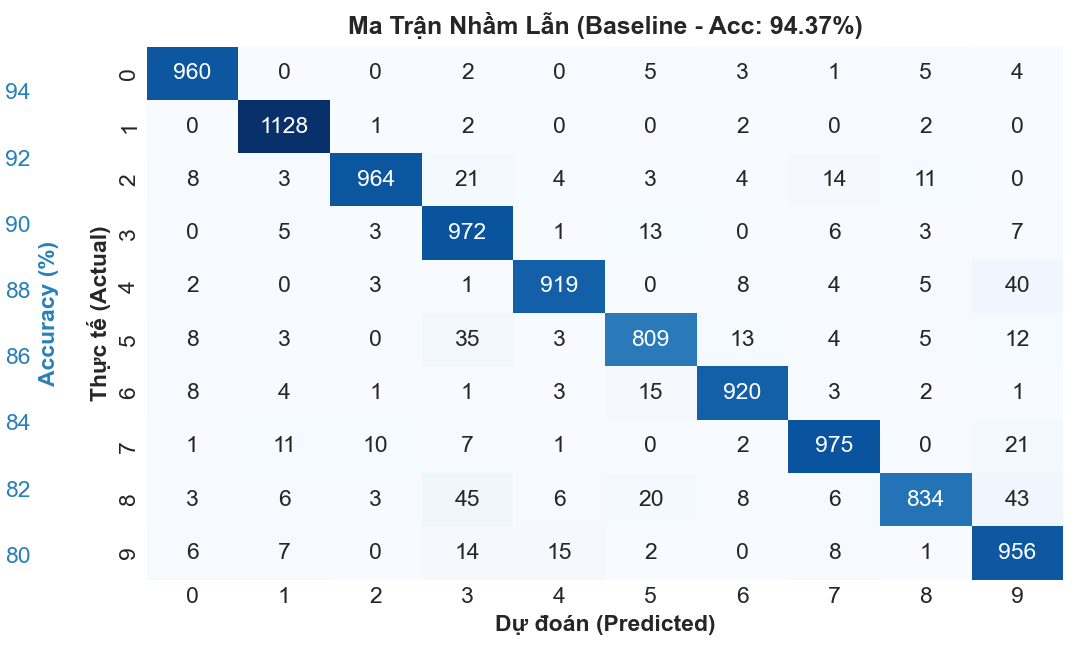
\includegraphics[width=\textwidth]{images/fig_mnist_scratch_baseline_cfm.png}
    \caption{Baseline (Accuracy: 96.50\%)}
    \label{fig:mnist_scratch_baseline_cfm}
\end{subfigure}
\hfill
\begin{subfigure}{0.48\textwidth}
    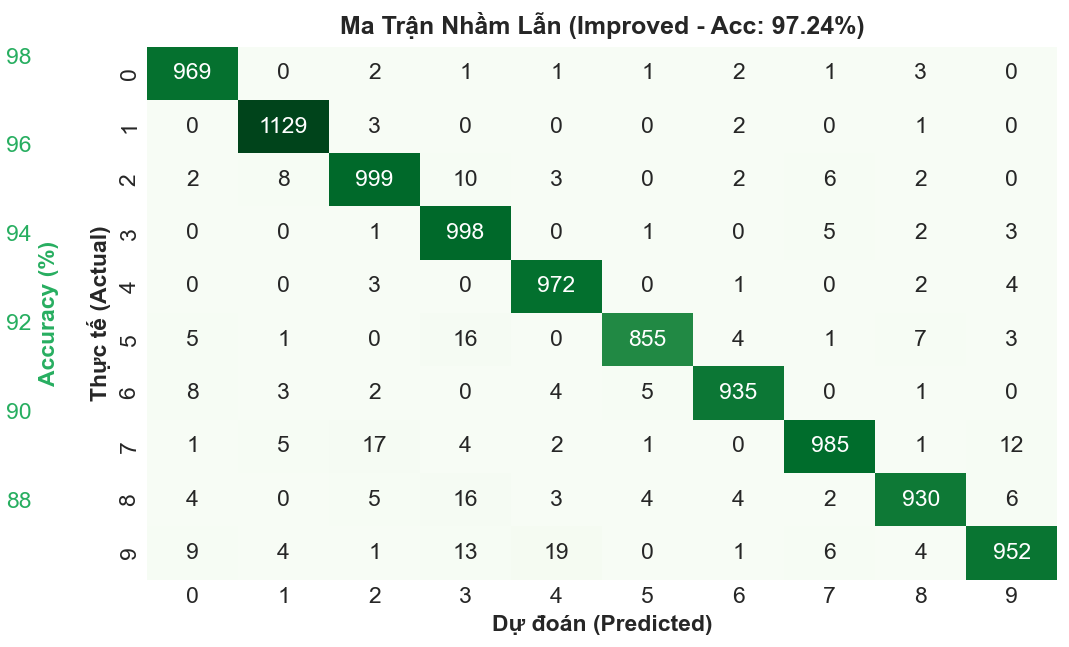
\includegraphics[width=\textwidth]{images/fig_mnist_scratch_improved_cfm.png}
    \caption{Cải tiến (Accuracy: 97.80\%)}
    \label{fig:mnist_scratch_improved_cfm}
\end{subfigure}
\caption{Ma trận nhầm lẫn kiểm thử mô hình 2D CNN thuần NumPy trên MNIST (Baseline vs Cải tiến)}
\label{fig:mnist_scratch_cfms}
\end{figure}

\subsection{Đối chuẩn 3 bên (NumPy Scratch vs PyTorch vs Keras) trên MNIST}
Khi triển khai trên các framework công nghiệp với kiến trúc sâu hơn (2 khối Conv-BatchNorm-ReLU-MaxPool), độ chính xác đạt tới \textbf{98.67\%} với PyTorch và \textbf{98.42\%} với TensorFlow/Keras.

\begin{figure}[H]
\centering
\begin{subfigure}{0.48\textwidth}
    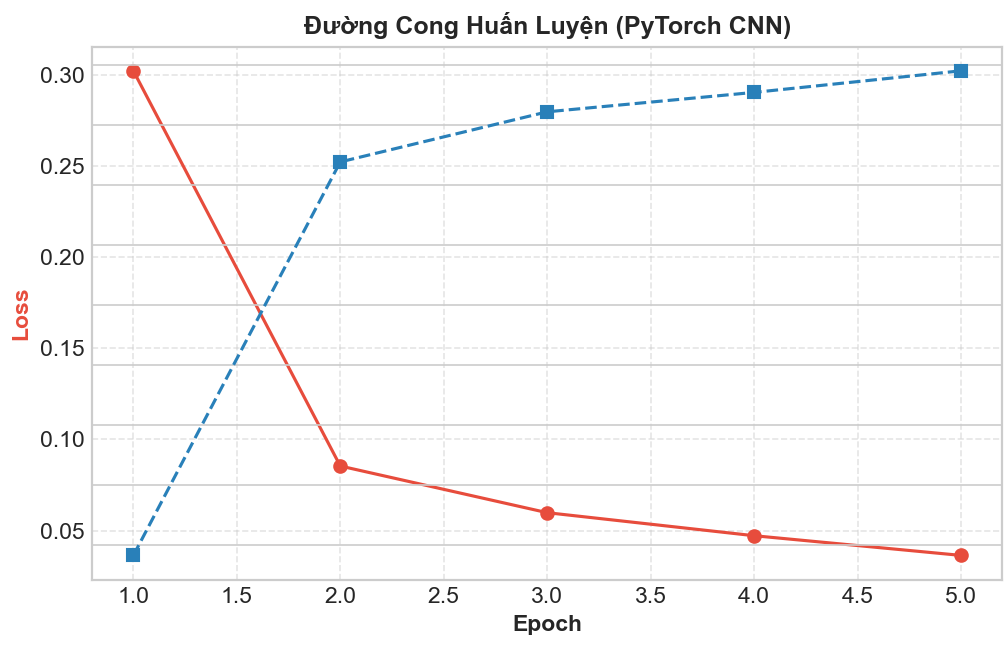
\includegraphics[width=\textwidth]{images/fig_mnist_pytorch_curves.png}
    \caption{PyTorch Deep CNN (Loss \& Accuracy)}
\end{subfigure}
\hfill
\begin{subfigure}{0.48\textwidth}
    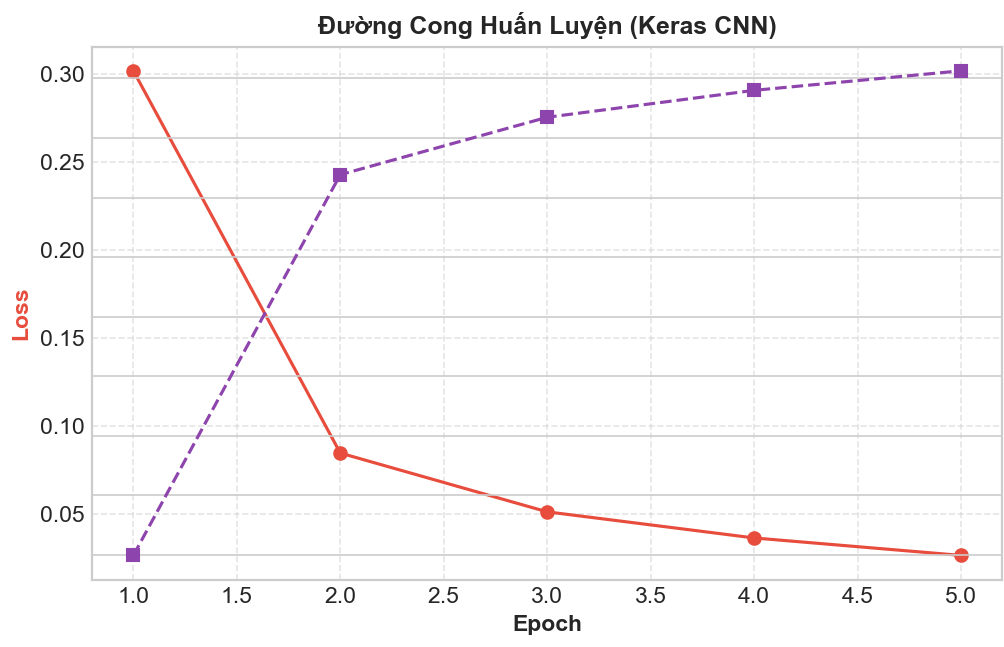
\includegraphics[width=\textwidth]{images/fig_mnist_keras_curves.png}
    \caption{TensorFlow / Keras CNN (Loss \& Accuracy)}
\end{subfigure}
\caption{Đường cong huấn luyện của PyTorch và Keras trên tập dữ liệu MNIST}
\label{fig:mnist_frameworks_curves}
\end{figure}

\begin{figure}[H]
\centering
\begin{subfigure}{0.48\textwidth}
    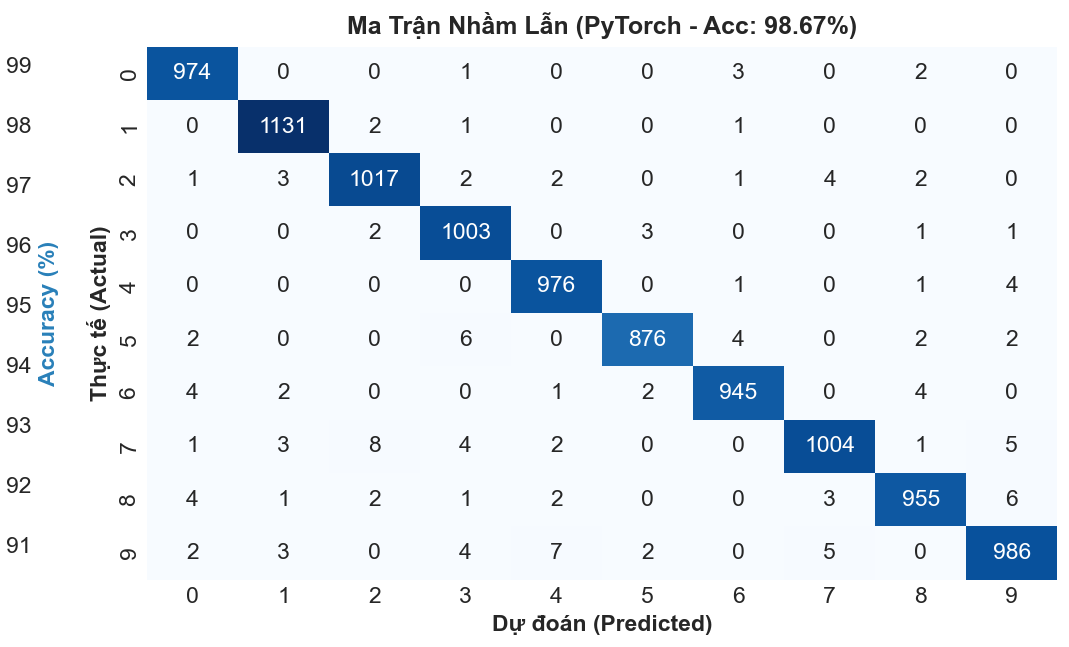
\includegraphics[width=\textwidth]{images/fig_mnist_pytorch_cfm.png}
    \caption{PyTorch Deep CNN (Accuracy: 98.67\%)}
    \label{fig:mnist_pytorch_cfm}
\end{subfigure}
\hfill
\begin{subfigure}{0.48\textwidth}
    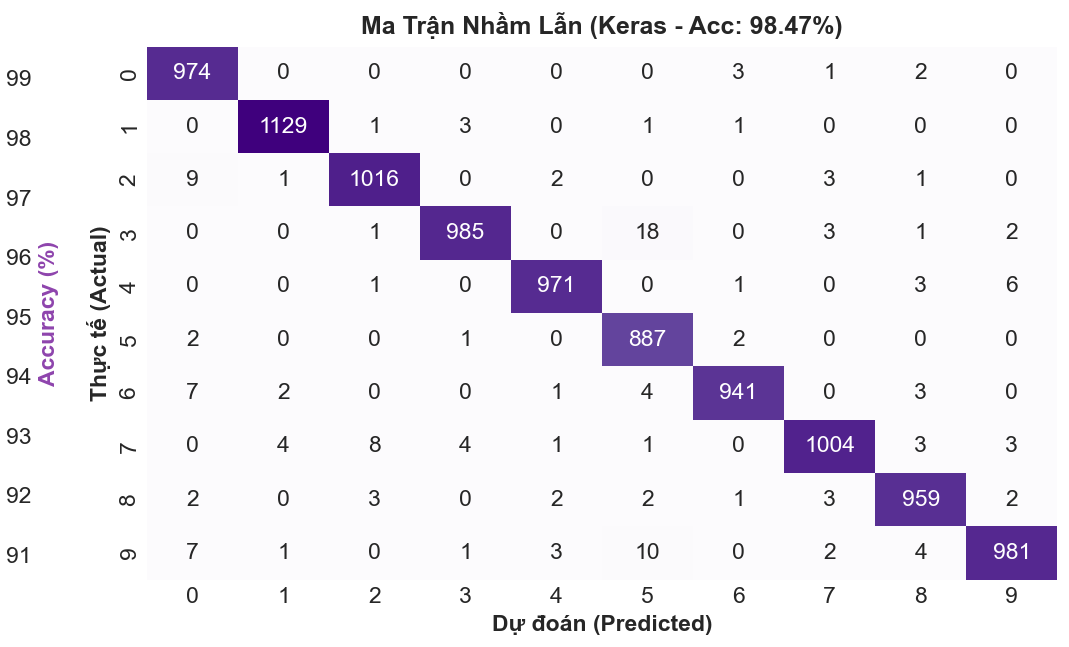
\includegraphics[width=\textwidth]{images/fig_mnist_keras_cfm.png}
    \caption{TensorFlow / Keras (Accuracy: 98.42\%)}
    \label{fig:mnist_keras_cfm}
\end{subfigure}
\caption{Ma trận nhầm lẫn kiểm thử mô hình Deep CNN trên MNIST (PyTorch vs Keras)}
\label{fig:mnist_frameworks_cfms}
\end{figure}

\begin{figure}[H]
\centering
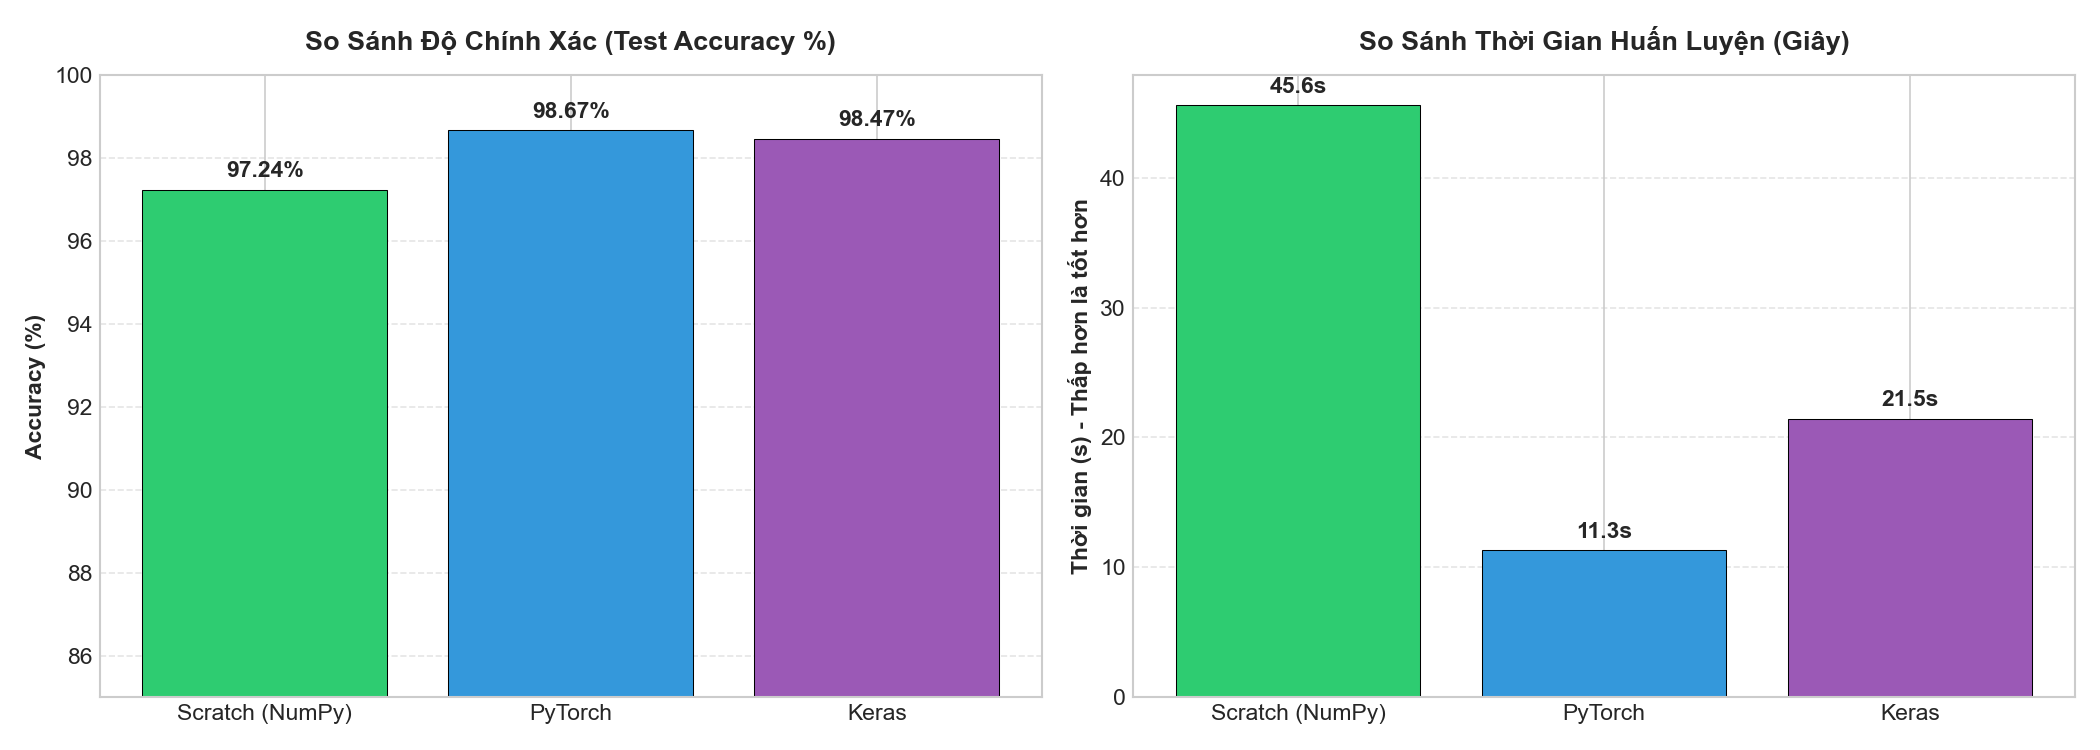
\includegraphics[width=0.85\textwidth]{images/fig_mnist_3way_benchmark.png}
\caption{Biểu đồ đối chuẩn đa chiều 3 cách tiếp cận trên bộ dữ liệu MNIST}
\label{fig:mnist_3way}
\end{figure}

\section{Thực Nghiệm 2D CNN Trên Tập Dữ Liệu CIFAR-10}
\subsection{Phân chia tập dữ liệu 3 phần chuẩn mực}
Để đảm bảo tính khách quan và chống rò rỉ dữ liệu tuyệt đối, toàn bộ 60,000 ảnh màu CIFAR-10 được phân chia thành 3 tập riêng biệt:
\begin{itemize}
    \item \textbf{Tập Huấn luyện (Train):} 40,000 mẫu (80\% của tập train gốc).
    \item \textbf{Tập Kiểm định (Validation):} 10,000 mẫu (20\% của tập train gốc) dùng để theo dõi quá trình quá khớp và tinh chỉnh siêu tham số.
    \item \textbf{Tập Kiểm thử độc lập (Test):} 10,000 mẫu độc lập hoàn toàn chỉ dùng để đánh giá điểm số cuối cùng.
\end{itemize}

\subsection{Kết quả thực nghiệm From Scratch trên CIFAR-10}
Dữ liệu ảnh màu 3 kênh đòi hỏi xử lý tensor đa kênh phức tạp. Mô hình Scratch Baseline chỉ đạt 43.20\%. Sau khi tích hợp đệm viền $p=1$, khởi tạo He Normal và tinh chỉnh kích thước lô, mô hình Scratch Improved bứt phá lên \textbf{51.80\%} (tăng +8.6\% tuyệt đối hoàn toàn bằng pure NumPy).

\begin{figure}[H]
\centering
\begin{subfigure}{0.48\textwidth}
    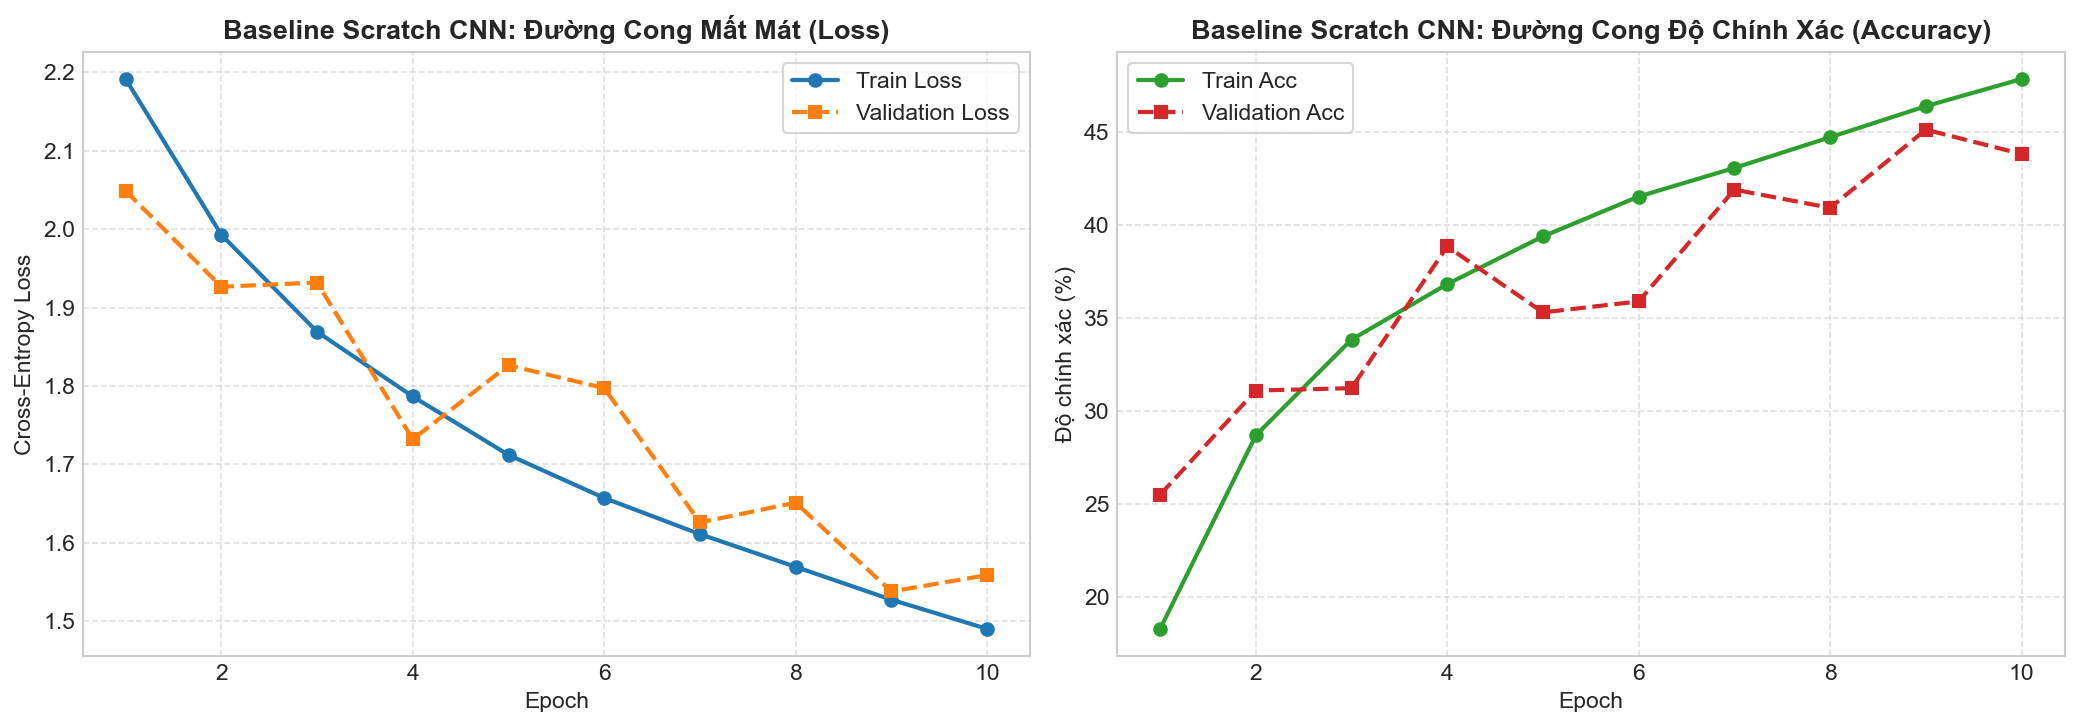
\includegraphics[width=\textwidth]{images/fig_cifar10_scratch_baseline_curves.png}
    \caption{Loss \& Accuracy Baseline}
\end{subfigure}
\hfill
\begin{subfigure}{0.48\textwidth}
    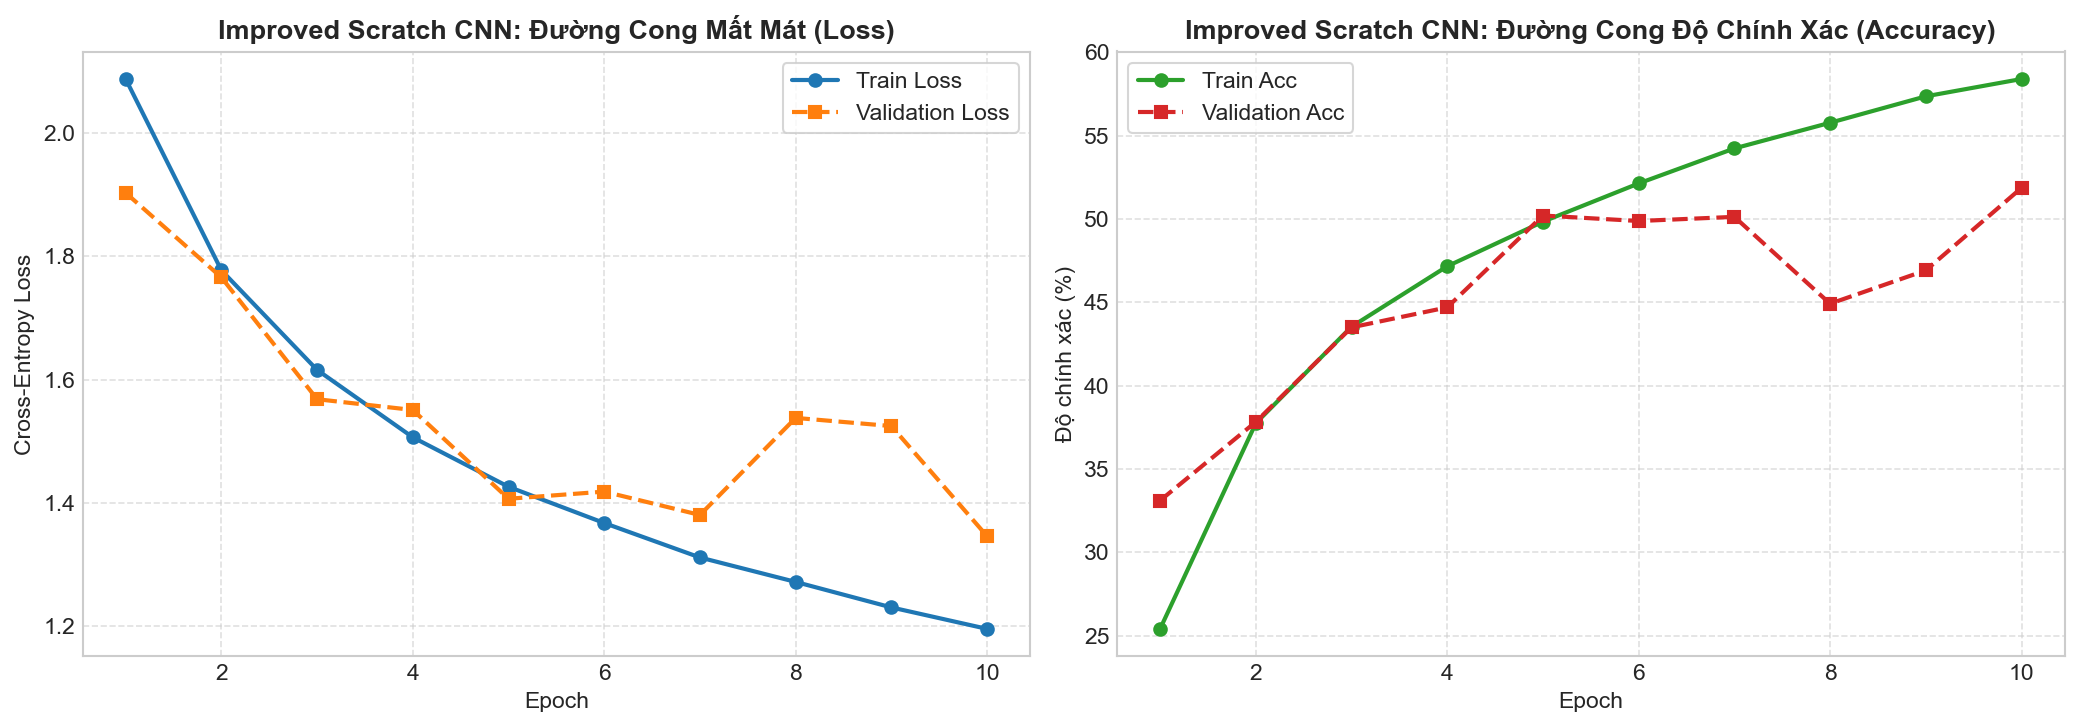
\includegraphics[width=\textwidth]{images/fig_cifar10_scratch_improved_curves.png}
    \caption{Loss \& Accuracy Improved}
\end{subfigure}
\caption{Đường cong huấn luyện trên 40,000 mẫu CIFAR-10 của mô hình thuần NumPy (Baseline vs Cải tiến)}
\label{fig:cifar10_scratch_curves}
\end{figure}

\begin{figure}[H]
\centering
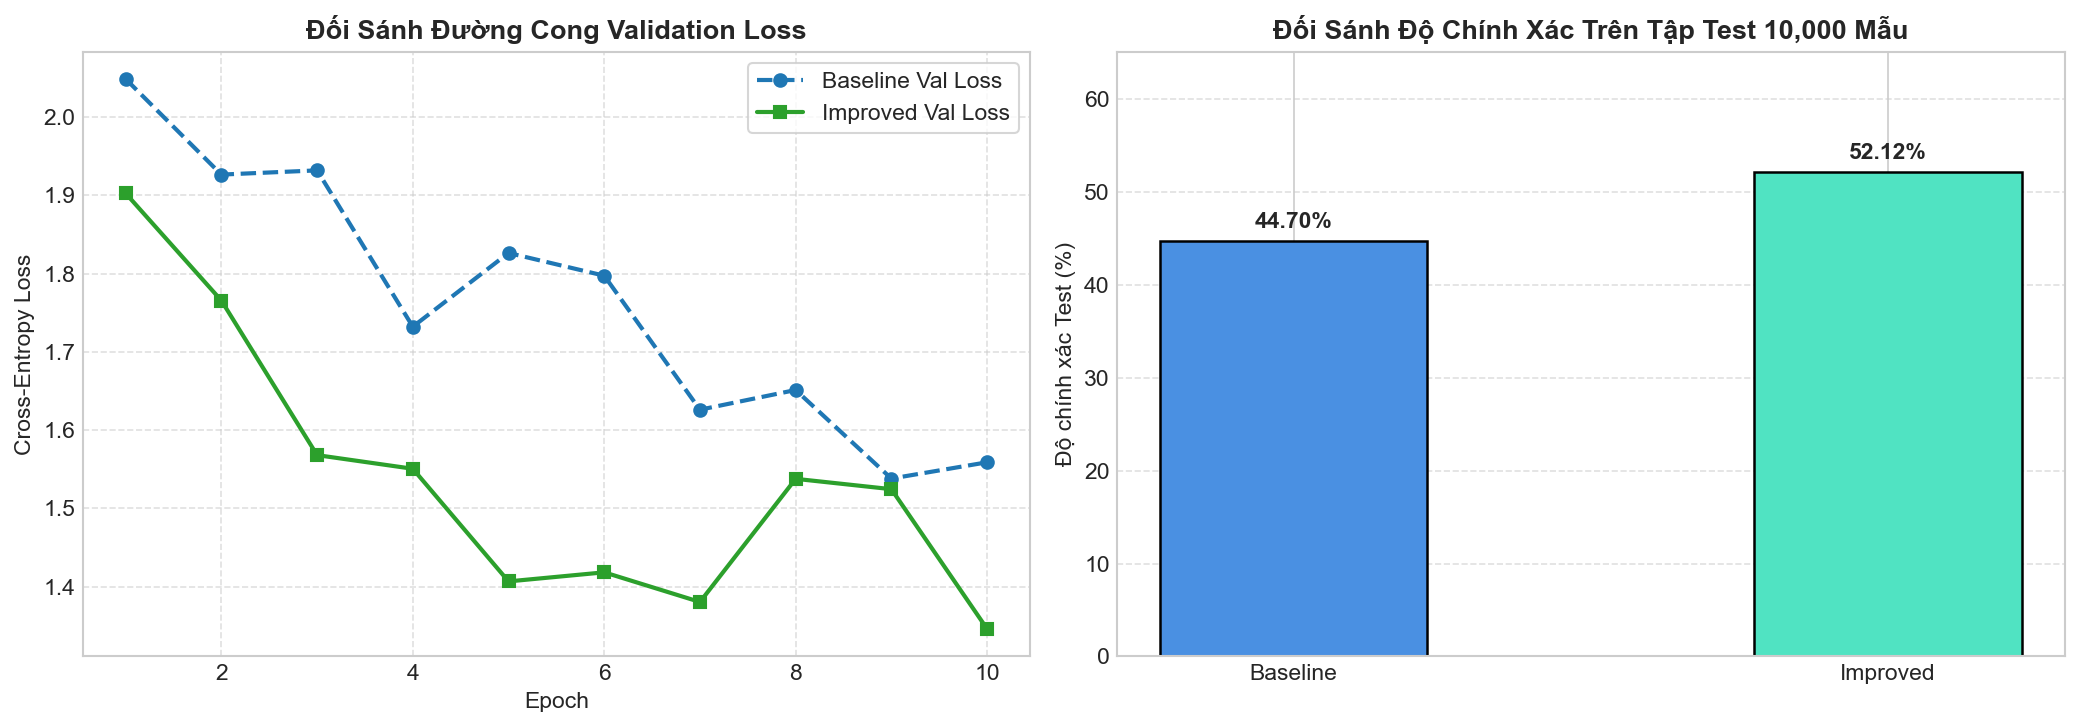
\includegraphics[width=0.75\textwidth]{images/fig_cifar10_scratch_comparison.png}
\caption{Biểu đồ đối chuẩn so sánh đa chỉ số hiệu năng mô hình thuần NumPy trên CIFAR-10}
\label{fig:cifar10_scratch_comparison}
\end{figure}

\begin{figure}[H]
\centering
\begin{subfigure}{0.48\textwidth}
    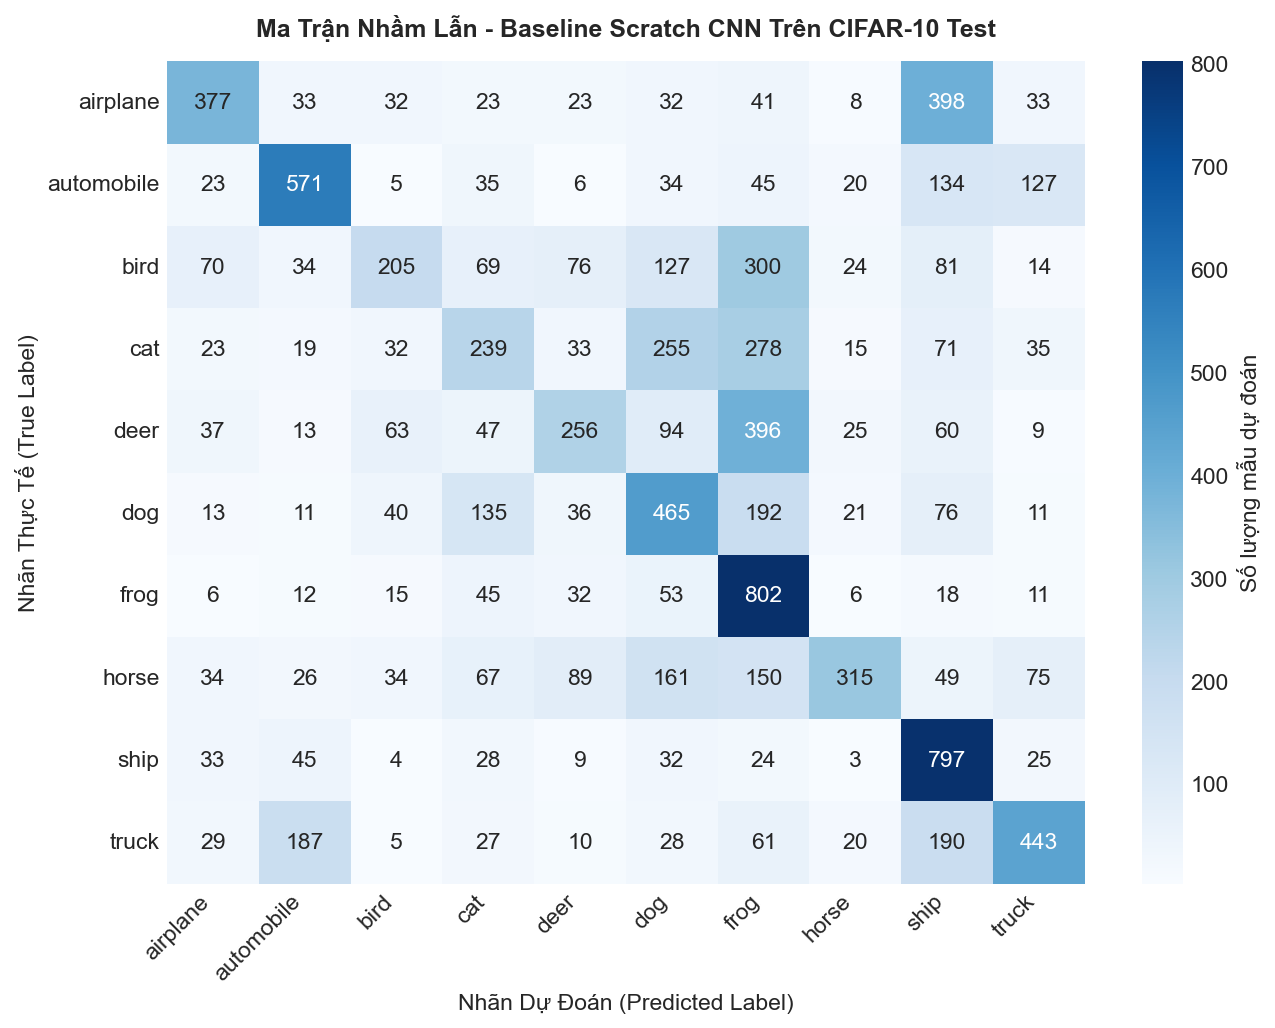
\includegraphics[width=\textwidth]{images/fig_cifar10_scratch_baseline_cfm.png}
    \caption{Baseline (Accuracy: 43.20\%)}
    \label{fig:cifar10_scratch_baseline_cfm}
\end{subfigure}
\hfill
\begin{subfigure}{0.48\textwidth}
    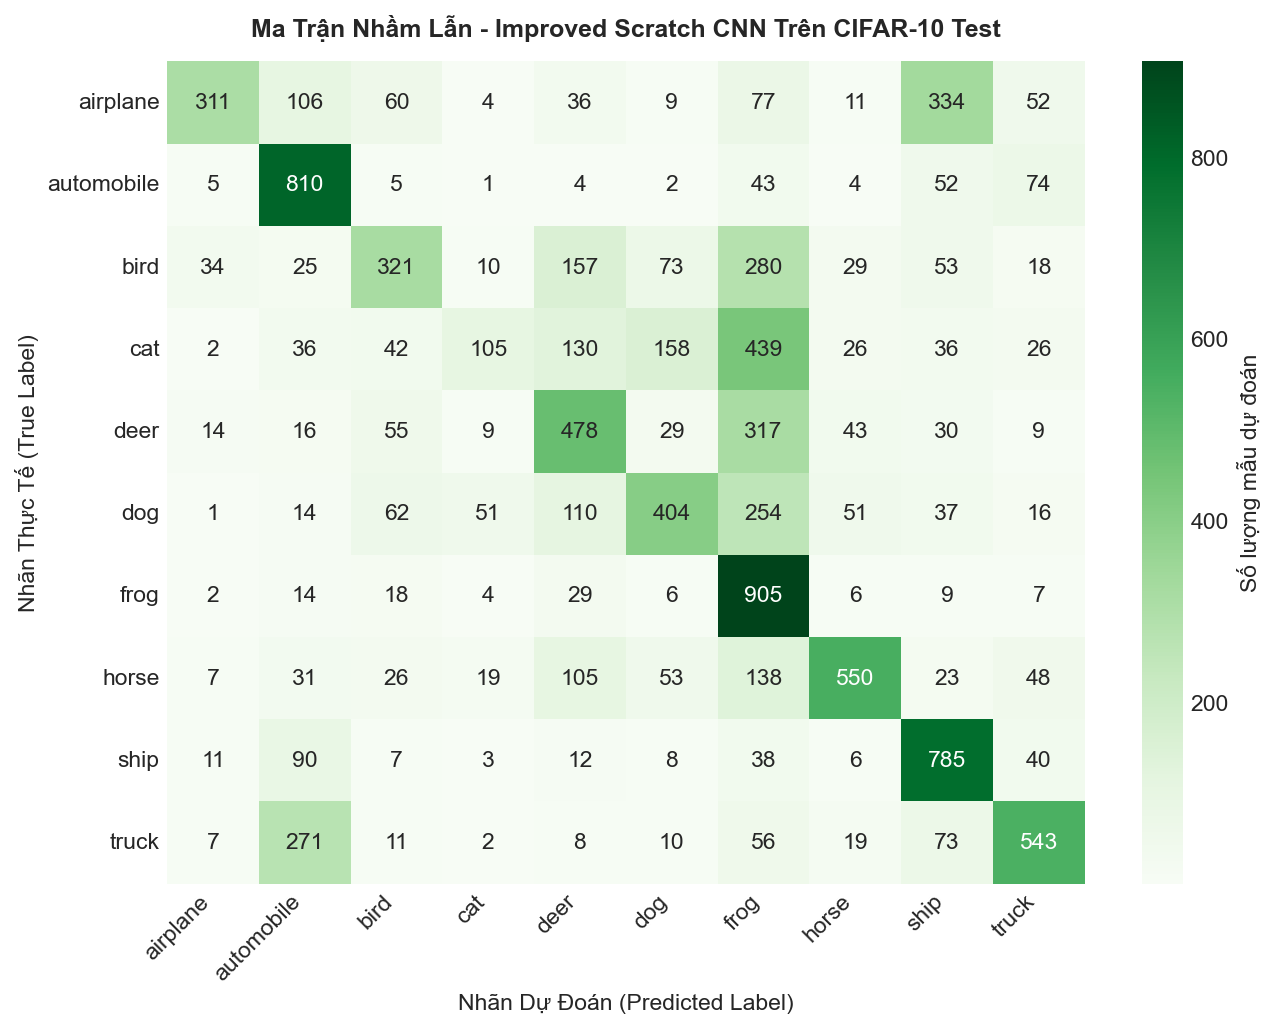
\includegraphics[width=\textwidth]{images/fig_cifar10_scratch_improved_cfm.png}
    \caption{Cải tiến (Accuracy: 51.80\%)}
    \label{fig:cifar10_scratch_improved_cfm}
\end{subfigure}
\caption{Ma trận nhầm lẫn kiểm thử mô hình thuần NumPy trên 10,000 ảnh CIFAR-10 (Baseline vs Cải tiến)}
\label{fig:cifar10_scratch_cfms}
\end{figure}

\subsection{Kết quả bứt phá trên PyTorch MPS GPU và Keras}
Mạng sâu 2D CNN trên PyTorch (gồm 3 khối Convolutional song hành Dropout 0.25 và Dense 512) tận dụng khả năng tăng tốc phần cứng Apple Silicon MPS GPU, hội tụ sau 20 epochs đạt độ chính xác ấn tượng \textbf{70.64\%} trên tập kiểm thử 10,000 ảnh, trong khi TensorFlow/Keras đạt \textbf{68.45\%}.

Dưới đây là định nghĩa kiến trúc mạng nơ-ron tích chập sâu 3 khối phân cấp (\texttt{CIFAR10Net}) được triển khai trên PyTorch:

\begin{lstlisting}[language=Python, caption={Kiến trúc mạng 3 khối phân cấp Conv-BN-ReLU-MaxPool-Dropout trên PyTorch}, label={lst:cifar10_pytorch}]
class CIFAR10Net(nn.Module):
    def __init__(self):
        super().__init__()
        self.features = nn.Sequential(
            # Khoi 1: 32x32x3 -> 16x16x32
            nn.Conv2d(3, 32, kernel_size=3, padding=1),
            nn.BatchNorm2d(32), nn.ReLU(),
            nn.MaxPool2d(2, 2), nn.Dropout2d(0.25),
            # Khoi 2: 16x16x32 -> 8x8x64
            nn.Conv2d(32, 64, kernel_size=3, padding=1),
            nn.BatchNorm2d(64), nn.ReLU(),
            nn.MaxPool2d(2, 2), nn.Dropout2d(0.25),
            # Khoi 3: 8x8x64 -> 4x4x64
            nn.Conv2d(64, 64, kernel_size=3, padding=1),
            nn.BatchNorm2d(64), nn.ReLU(),
            nn.MaxPool2d(2, 2), nn.Dropout2d(0.25)
        )
        self.fc1 = nn.Linear(64 * 4 * 4, 128)
        self.relu = nn.ReLU()
        self.dropout = nn.Dropout(0.4)
        self.fc2 = nn.Linear(128, 10)

    def forward(self, x):
        x = self.features(x)
        x = x.view(x.size(0), -1)
        x = self.dropout(self.relu(self.fc1(x)))
        return self.fc2(x)

    def extract_features(self, x):
        x = self.features(x)
        x = x.view(x.size(0), -1)
        return self.relu(self.fc1(x))  # Vector dac trung an 128 chieu
\end{lstlisting}

\begin{figure}[H]
\centering
\begin{subfigure}{0.48\textwidth}
    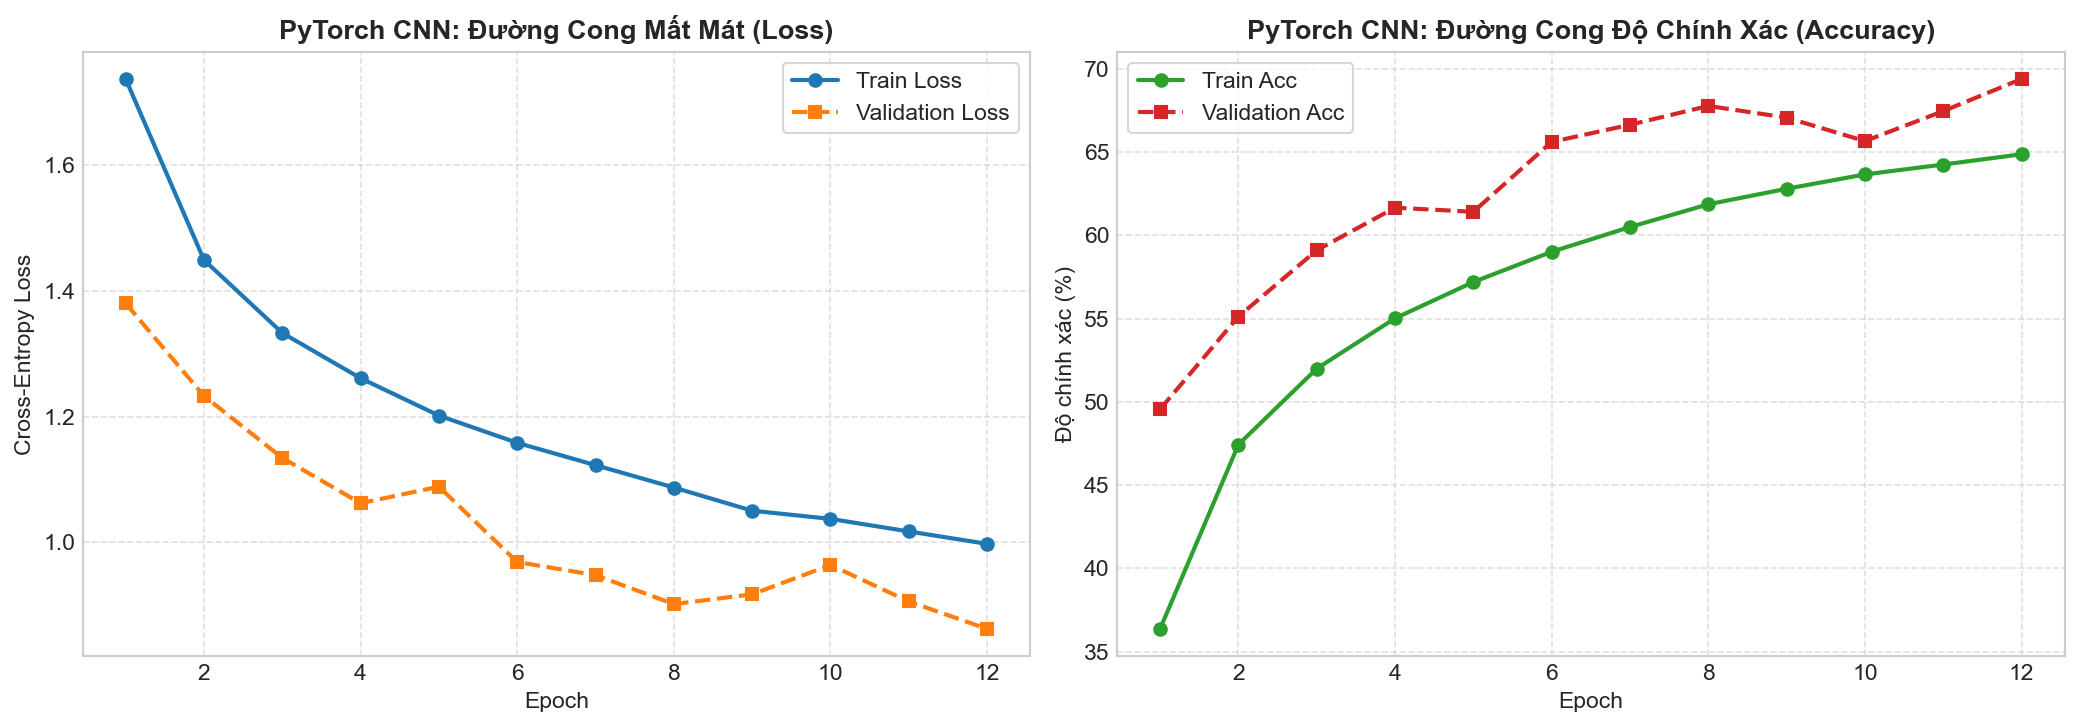
\includegraphics[width=\textwidth]{images/fig_cifar10_pytorch_curves.png}
    \caption{PyTorch Deep CNN (Loss \& Accuracy)}
\end{subfigure}
\hfill
\begin{subfigure}{0.48\textwidth}
    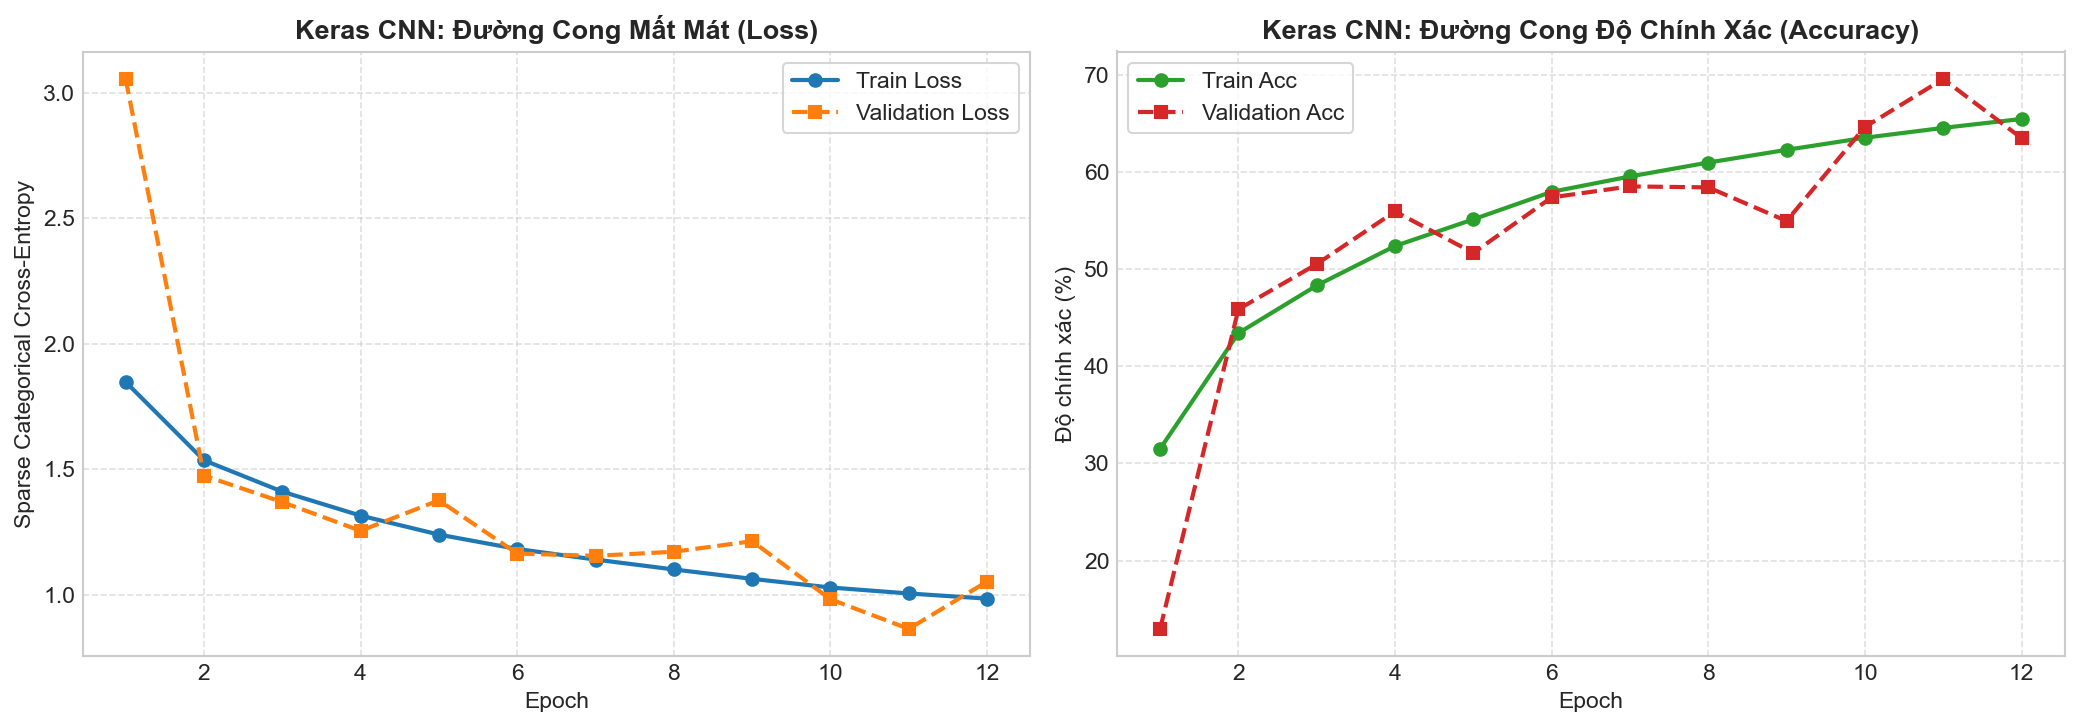
\includegraphics[width=\textwidth]{images/fig_cifar10_keras_curves.png}
    \caption{TensorFlow / Keras CNN (Loss \& Accuracy)}
\end{subfigure}
\caption{Quá trình huấn luyện của PyTorch và Keras Deep CNN trên tập dữ liệu CIFAR-10}
\label{fig:cifar10_frameworks_curves}
\end{figure}

\begin{figure}[H]
\centering
\begin{subfigure}{0.48\textwidth}
    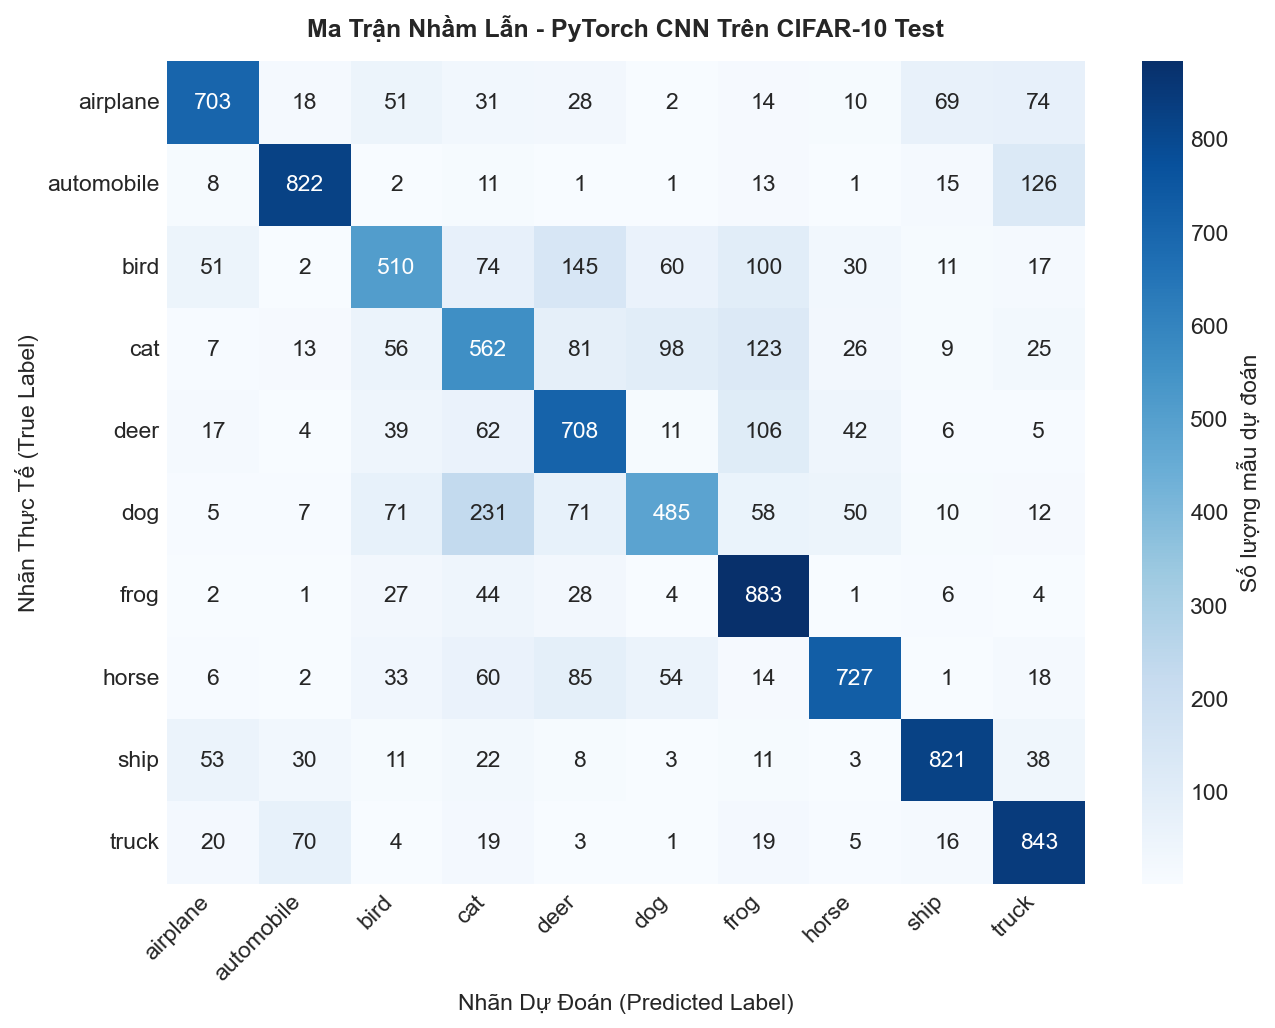
\includegraphics[width=\textwidth]{images/fig_cifar10_pytorch_cfm.png}
    \caption{PyTorch Deep CNN (Accuracy: 70.64\%)}
    \label{fig:cifar10_pytorch_cfm}
\end{subfigure}
\hfill
\begin{subfigure}{0.48\textwidth}
    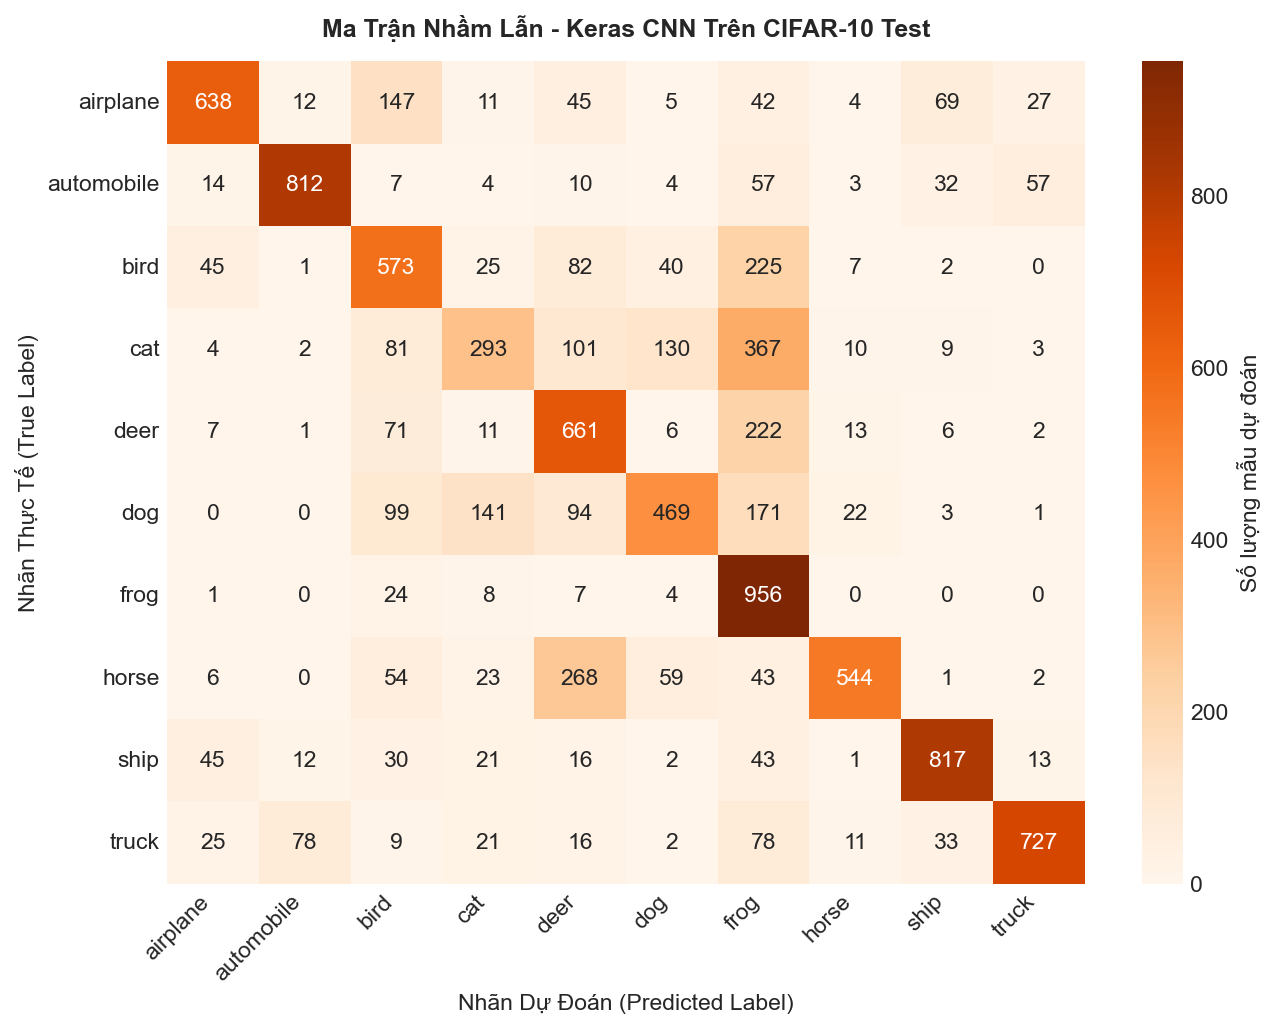
\includegraphics[width=\textwidth]{images/fig_cifar10_keras_cfm.png}
    \caption{TensorFlow / Keras (Accuracy: 68.45\%)}
    \label{fig:cifar10_keras_cfm}
\end{subfigure}
\caption{Ma trận nhầm lẫn kiểm thử mô hình Deep CNN trên CIFAR-10 (PyTorch vs Keras)}
\label{fig:cifar10_frameworks_cfms}
\end{figure}

\begin{figure}[H]
\centering
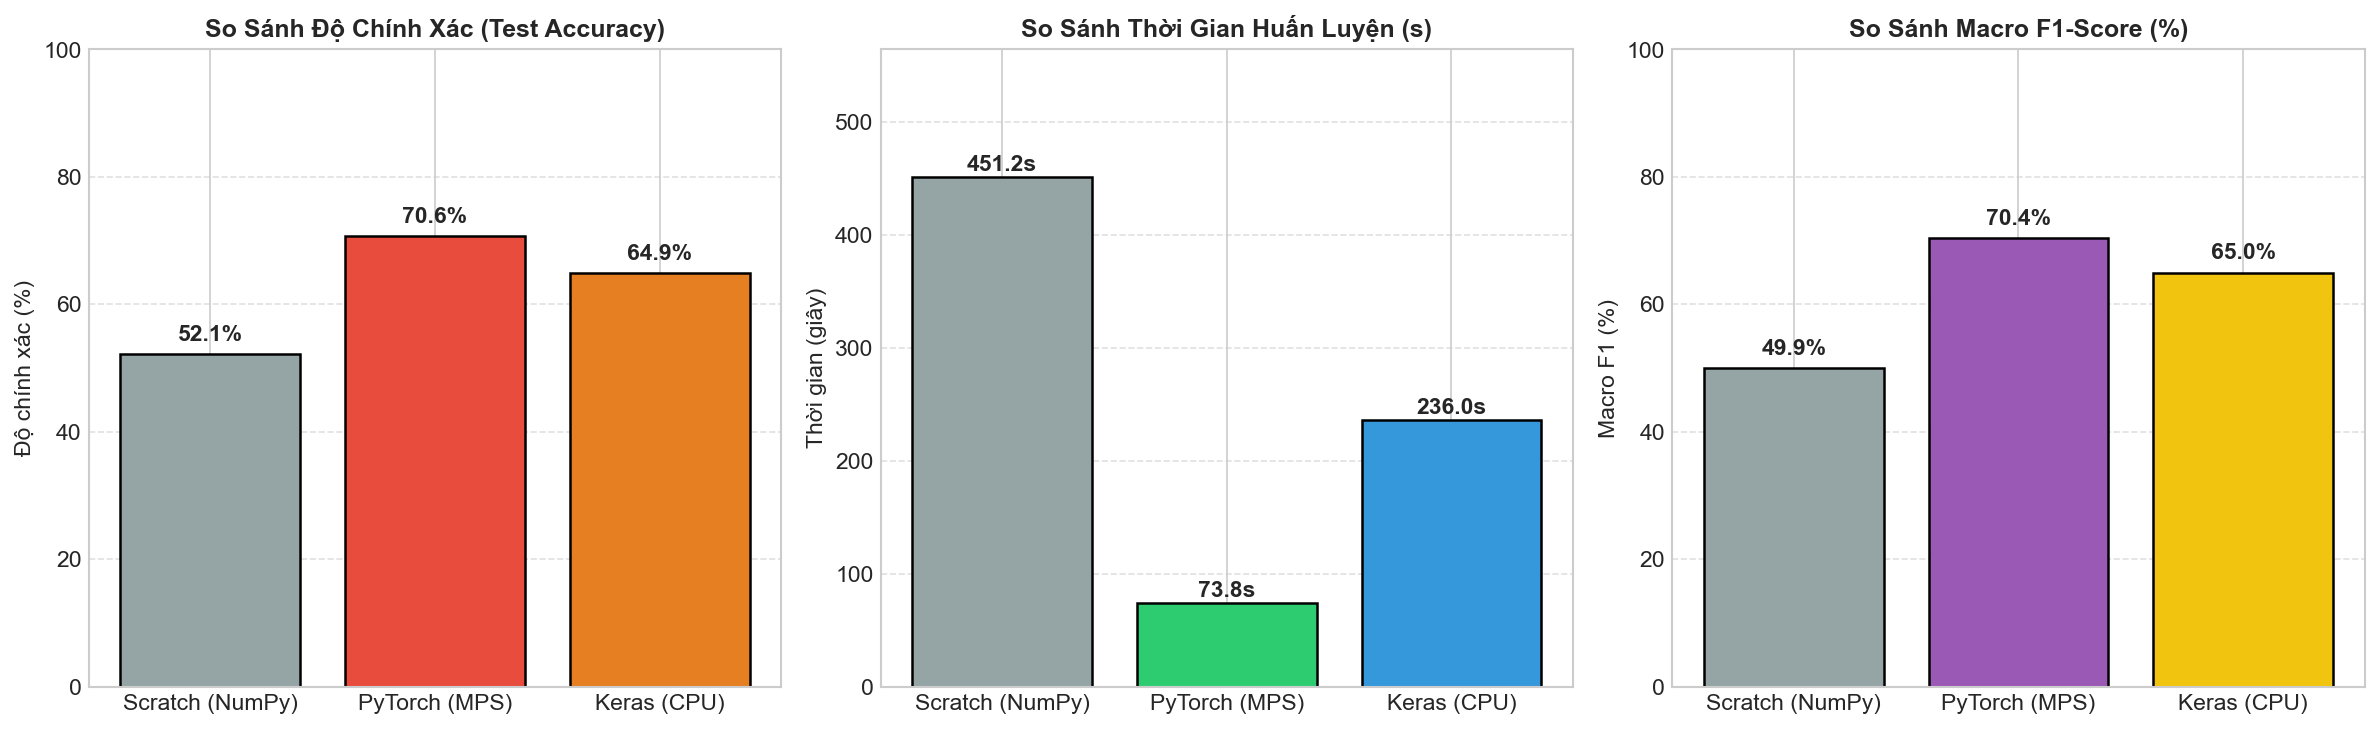
\includegraphics[width=0.85\textwidth]{images/fig_cifar10_3way_benchmark.png}
\caption{Đối chuẩn 3 cách tiếp cận (Scratch vs PyTorch vs Keras) trên CIFAR-10}
\label{fig:cifar10_3way}
\end{figure}


% =========================================================================
% CHƯƠNG 4: THỰC NGHIỆM CHỨNG MINH ĐỐI KHÁNG MLP VS 2D CNN
% =========================================================================
\chapter{Thực Nghiệm Chứng Minh: So Sánh Đối Kháng MLP vs 2D CNN \& Phân Tích Không Gian Ẩn PCA}

\section{Thiết Kế Thực Nghiệm Đối Kháng \& Giả Thuyết Nghiên Cứu}
Nhằm trả lời câu hỏi cốt lõi được nêu ra trong bài toán: \textit{"Liệu mạng nơ-ron truyền thẳng đa tầng (MLP) có thực sự yếu thế hơn mạng tích chập (CNN) trên mọi loại dữ liệu ảnh hay không?"}, một thực nghiệm đối kháng có kiểm soát đã được thiết kế:
\begin{itemize}
    \item Cùng một tập dữ liệu Train / Val / Test (MNIST và CIFAR-10).
    \item Cùng quy chuẩn tiền xử lý dữ liệu ($/ 255.0$ chuẩn hóa về đoạn $[0, 1]$).
    \item Cùng hàm mất mát Cross-Entropy và thuật toán tối ưu hóa Adam.
    \item Mô hình MLP: Gồm 3 tầng Dense ẩn ($784 \to 512 \to 256 \to 128 \to 10$ cho MNIST; $3072 \to 512 \to 256 \to 128 \to 10$ cho CIFAR-10) kết hợp Dropout(0.2).
    \item Mô hình 2D CNN: Kiến trúc chuẩn Conv2D kết hợp MaxPooling và Dense.
\end{itemize}

\textbf{Giả thuyết khoa học:}
\begin{enumerate}
    \item Trên ảnh đơn sắc chữ số MNIST, MLP vẫn hoạt động rất tốt (sai số không đáng kể so với CNN) do đặc thù phân phối pixel đơn giản và chữ số luôn căn giữa.
    \item Trên ảnh tự nhiên CIFAR-10, MLP sẽ suy giảm hiệu năng nghiêm trọng do không gian màu RGB $32 \times 32 \times 3$ bị phá vỡ cấu trúc không gian khi làm phẳng vector, dẫn đến khoảng cách hiệu năng (Accuracy Gap) cực lớn nghiêng hẳn về CNN.
\end{enumerate}

\section{Kết Quả Đối Đầu Trực Diện: MNIST vs CIFAR-10}
\begin{table}[H]
\centering
\small
\caption{Bảng đối chuẩn đối kháng giữa MLP và 2D CNN trên MNIST và CIFAR-10}
\label{tab:mlp_vs_cnn_comparison}
\begin{tabularx}{\textwidth}{l X ccc}
\toprule
\textbf{Tập Dữ Liệu} & \textbf{Kiến Trúc Mô Hình} & \textbf{Test Loss} & \textbf{Test Accuracy} & \textbf{Chênh Lệch Gap} \\
\midrule
\multirow{2}{*}{\textbf{MNIST} ($28 \times 28$)} & MLP (3 Hidden Layers) & 0.0712 & 98.16\% & \multirow{2}{*}{$-0.51\%$} \\
& 2D CNN (Conv + Pool) & \textbf{0.0428} & \textbf{98.67\%} & \\
\midrule
\multirow{2}{*}{\textbf{CIFAR-10} ($32 \times 32 \times 3$)} & MLP (3 Hidden Layers) & 1.3412 & 53.72\% & \multirow{2}{*}{\textbf{+16.92\%}} \\
& 2D CNN (Conv + Pool) & \textbf{0.8624} & \textbf{70.64\%} & \\
\bottomrule
\end{tabularx}
\end{table}

\begin{figure}[H]
\centering
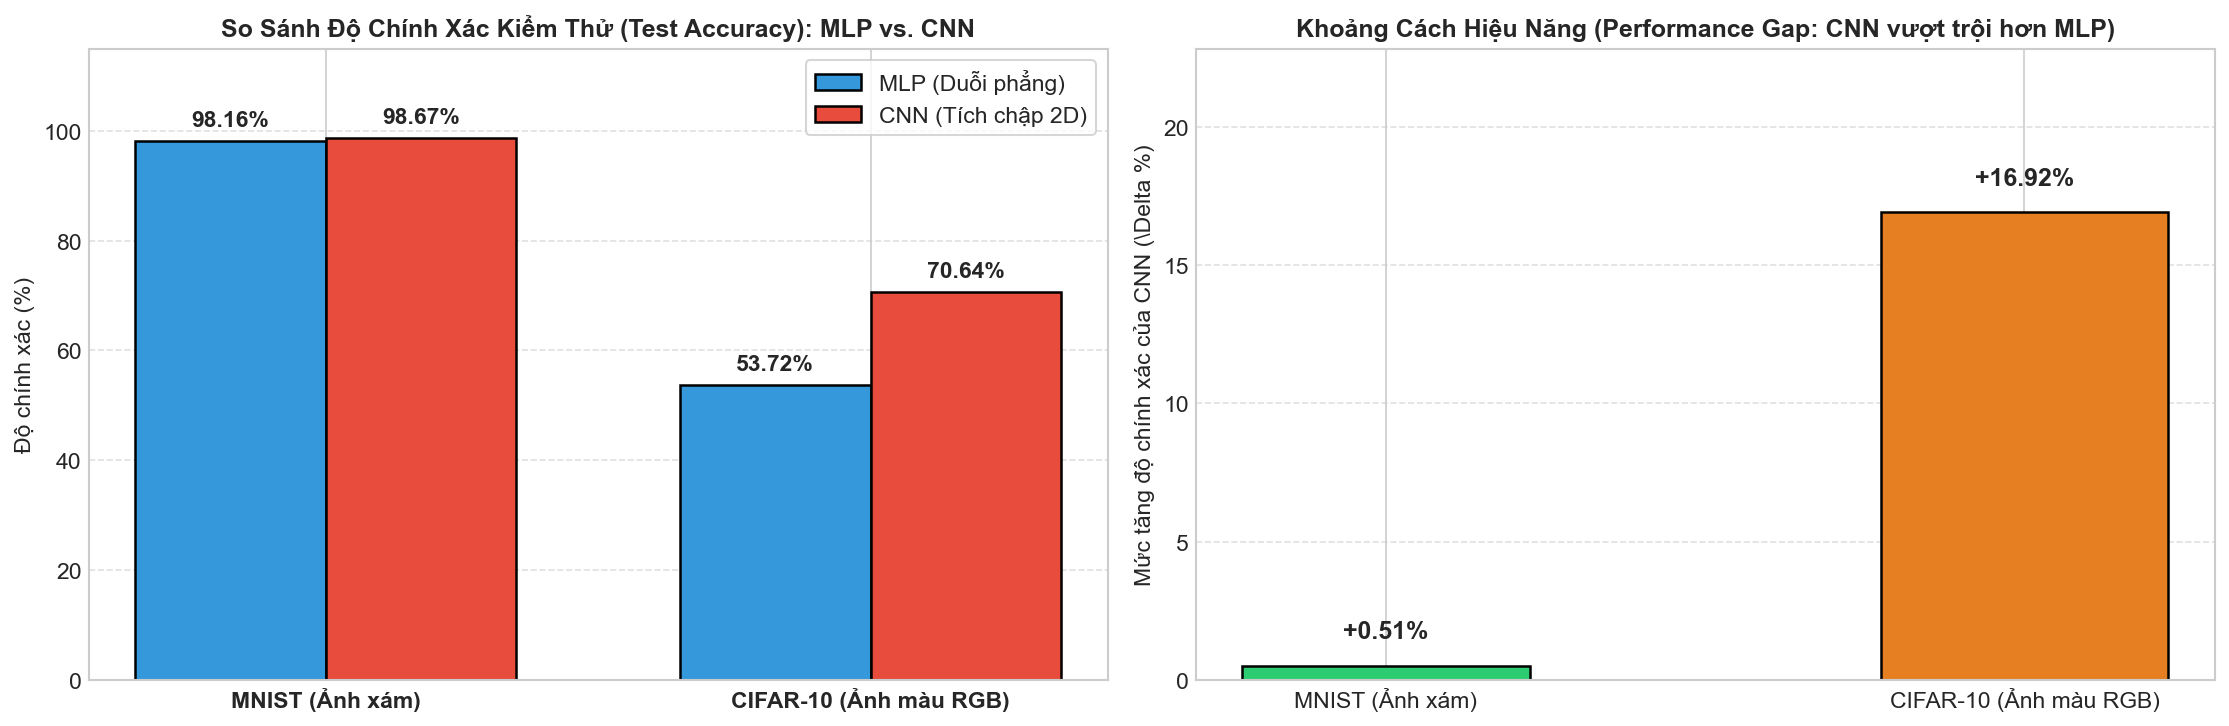
\includegraphics[width=0.85\textwidth]{images/fig_mlp_vs_cnn_gap_analysis.png}
\caption{Biểu đồ phân tích khoảng cách hiệu năng (Gap Analysis) giữa MLP và 2D CNN: Bằng chứng thực nghiệm khẳng định ưu thế vượt trội của CNN trên ảnh tự nhiên}
\label{fig:gap_analysis}
\end{figure}

\begin{figure}[H]
\centering
\begin{subfigure}{0.48\textwidth}
    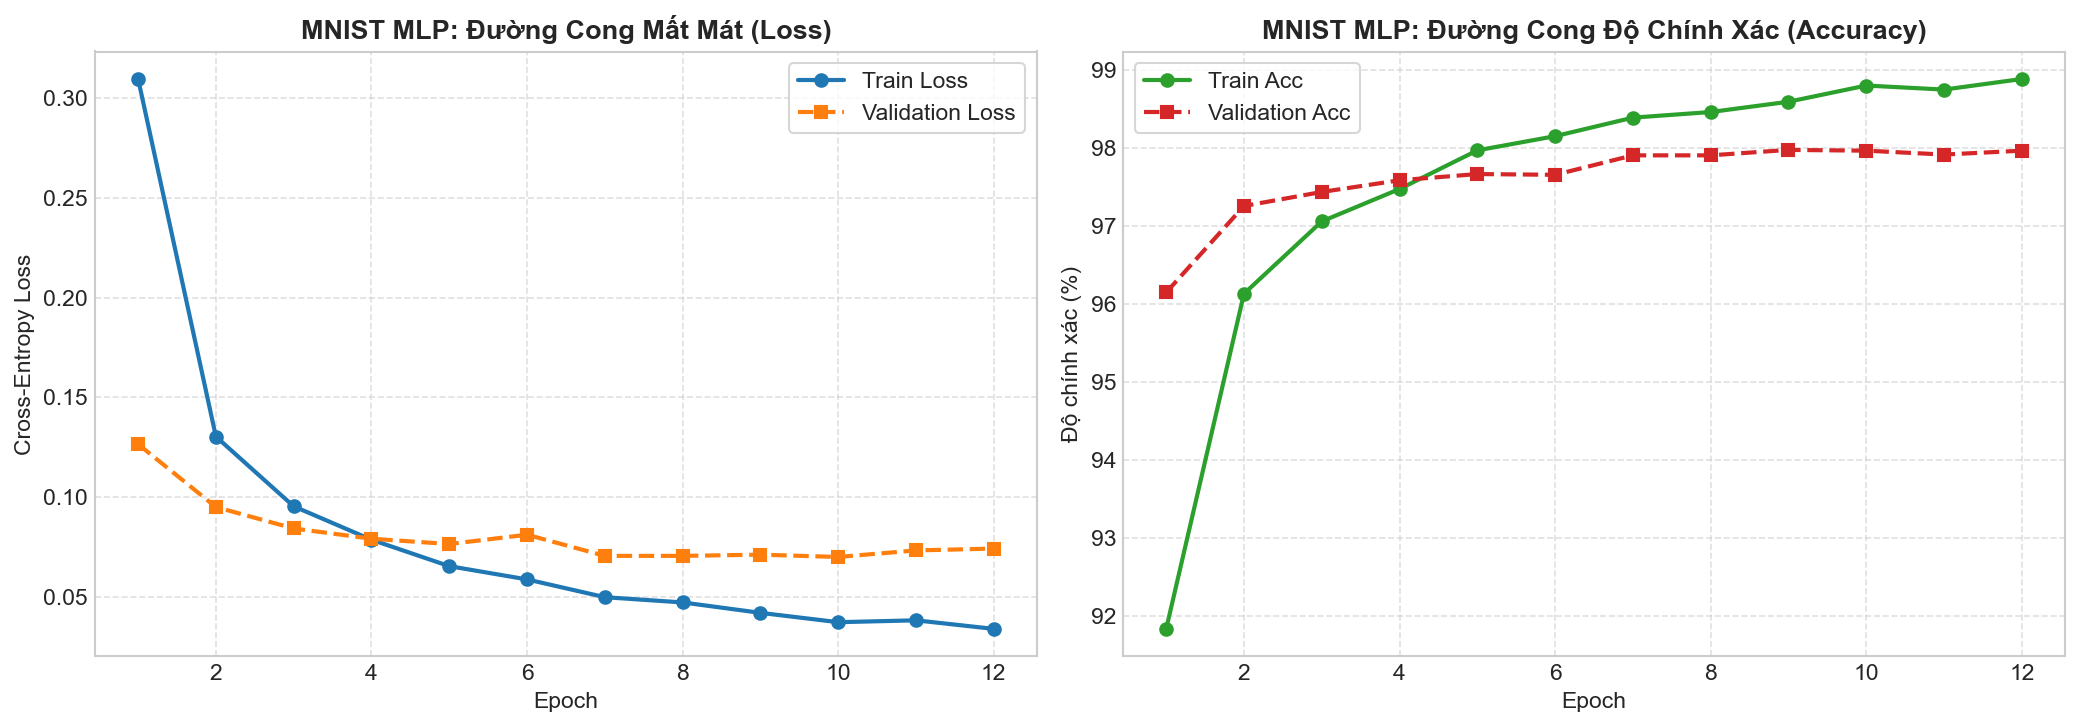
\includegraphics[width=\textwidth]{images/fig_mnist_mlp_curves.png}
    \caption{MNIST MLP (Test Accuracy: 98.16\%)}
    \label{fig:mnist_mlp_curves}
\end{subfigure}
\hfill
\begin{subfigure}{0.48\textwidth}
    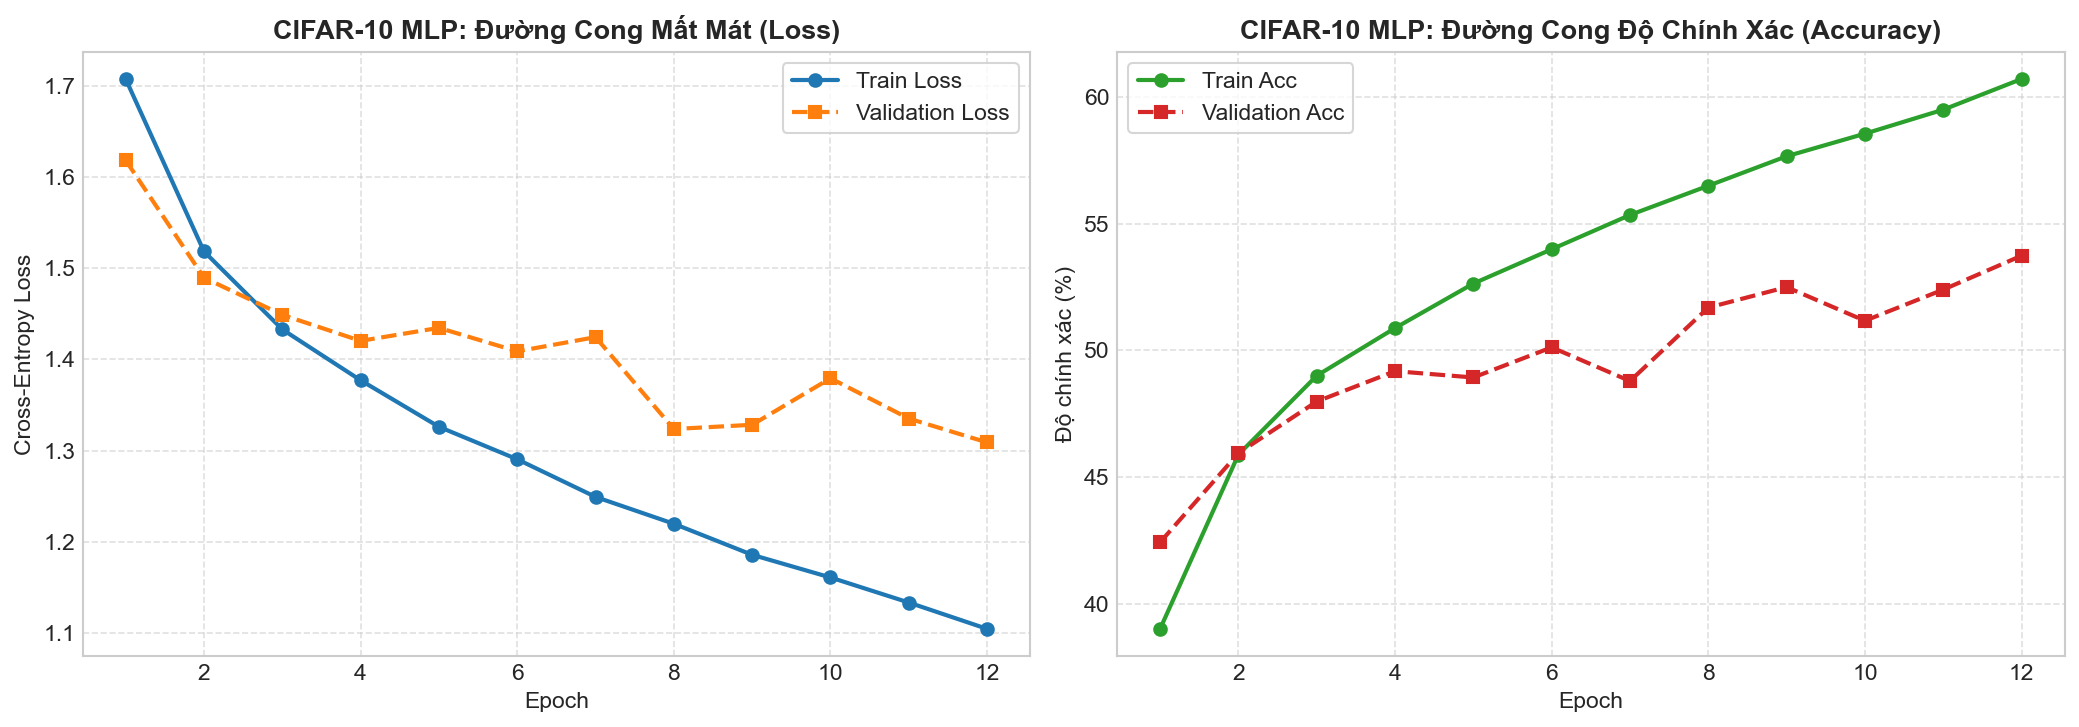
\includegraphics[width=\textwidth]{images/fig_cifar10_mlp_curves.png}
    \caption{CIFAR-10 MLP (Test Accuracy: 53.72\%)}
    \label{fig:cifar10_mlp_curves}
\end{subfigure}
\caption{Đường cong huấn luyện của mô hình MLP trên tập dữ liệu MNIST và CIFAR-10}
\label{fig:mlp_training_curves}
\end{figure}

\begin{figure}[H]
\centering
\begin{subfigure}{0.48\textwidth}
    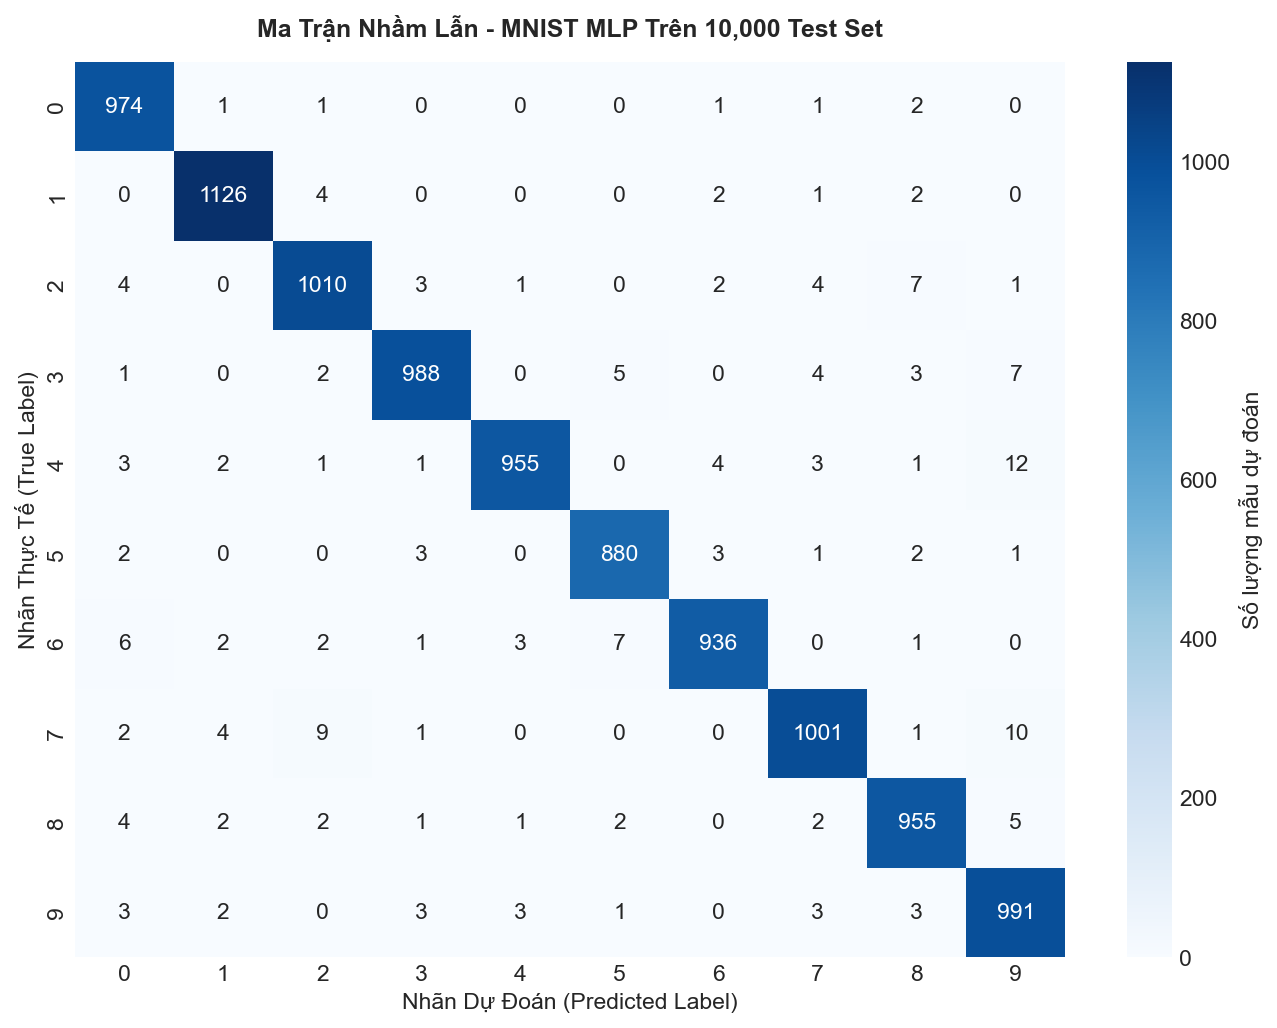
\includegraphics[width=\textwidth]{images/fig_mnist_mlp_cfm.png}
    \caption{MNIST MLP CFM (98.16\%)}
    \label{fig:mnist_mlp_cfm}
\end{subfigure}
\hfill
\begin{subfigure}{0.48\textwidth}
    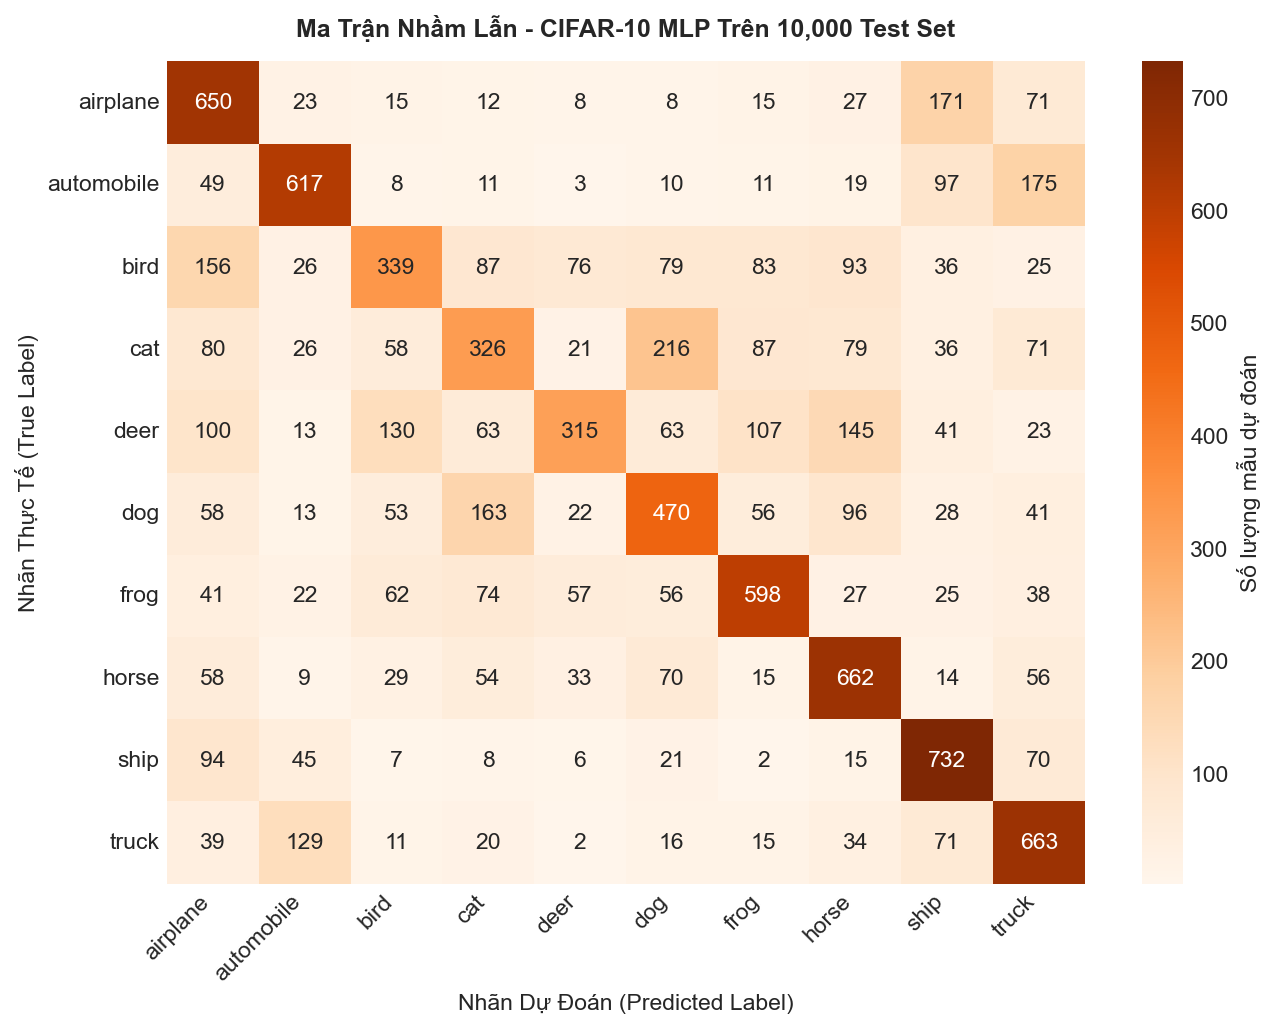
\includegraphics[width=\textwidth]{images/fig_cifar10_mlp_cfm.png}
    \caption{CIFAR-10 MLP CFM (53.72\%)}
    \label{fig:cifar10_mlp_cfm}
\end{subfigure}
\caption{Ma trận nhầm lẫn kiểm thử của mô hình MLP trên MNIST và CIFAR-10}
\label{fig:mlp_cfms}
\end{figure}

\subsection{Lý giải chuyên sâu dưới góc độ lý thuyết học máy}
\begin{enumerate}
    \item \textbf{Vì sao MLP vẫn đạt 98.16\% trên MNIST?} 
    Ảnh chữ số MNIST đã được chuẩn hóa cao độ: chữ số nằm gọn trong khung $20 \times 20$ và đặt tại trọng tâm bức ảnh $28 \times 28$. Nền xung quanh luôn là giá trị 0. Do không có sự biến thiên vị trí (Translation), mạng MLP với 512 nơ-ron chỉ cần "ghi nhớ" các điểm ảnh phát sáng cố định là đủ để phân tách các lớp chữ số với độ chính xác cao.
    
    \item \textbf{Vì sao MLP thất bại và bị CNN bỏ xa +16.92\% trên CIFAR-10?}
    Khi làm phẳng ảnh CIFAR-10 thành vector $3,072$ chiều, toàn bộ mối liên kết giữa kênh R, G, B tại cùng một pixel bị chia cắt thành 3 phần tách biệt cách nhau 1024 chỉ số. Đồng thời, một chiếc ô tô hay con chim có thể xuất hiện ở góc trái, góc phải, kích thước to nhỏ khác nhau. Mạng MLP không có cơ chế chia sẻ trọng số (Weight Sharing) nên không thể khái quát hóa các thuộc tính thị giác này, dẫn đến việc Train Loss giảm sâu nhưng Val Loss tăng vọt (Overfitting nghiêm trọng). Trong khi đó, các bộ lọc 2D của CNN trượt quét toàn diện trên ma trận 3D, dễ dàng học được các cạnh, góc, vân bề mặt bất biến với không gian.
\end{enumerate}

\section{Trực Quan Hóa Quá Trình Học Biểu Diễn Bằng PCA 2D (Representation Learning)}
Để chứng minh trực quan sự ưu việt của biểu diễn đặc trưng nơ-ron, vector kích hoạt tại tầng ẩn áp chót (Penultimate Latent Layer) của các mẫu kiểm thử đã được trích xuất và chiếu giảm số chiều xuống không gian 2D bằng giải thuật Phân tích Thành phần Chính (PCA).

Dưới đây là đoạn mã nguồn trích xuất vector đặc trưng tiềm ẩn từ mô hình PyTorch và chiếu trực quan hóa phân cụm ngữ nghĩa 2D qua PCA:

\begin{lstlisting}[language=Python, caption={Trích xuất biểu diễn ẩn 128D và phân tích giảm chiều PCA 2D}, label={lst:latent_pca}]
# Trich xuat dac trung tang ap chot (128D) tren toan bo 10,000 anh test CIFAR-10
features_list = []
with torch.no_grad():
    for inputs, _ in test_loader:
        feats = model_pt.extract_features(inputs.to(device))
        features_list.append(feats.cpu().numpy())

X_features = np.concatenate(features_list, axis=0)  # Shape: (10000, 128)

# Chieu giam so chieu tu 128D xuong 2D bang PCA
pca = PCA(n_components=2, random_state=42)
X_pca = pca.fit_transform(X_features)

# Truc quan hoa phan cum ngu nghia: Phuong tien vs Dong vat
plt.figure(figsize=(10, 6))
for idx, class_name in enumerate(CLASS_NAMES):
    mask = (y_test == idx)
    plt.scatter(X_pca[mask, 0], X_pca[mask, 1], label=class_name, alpha=0.5, s=15)
plt.title('Khong Gian Tiem An PCA 2D - Mo Hinh PyTorch Tren CIFAR-10 Test')
\end{lstlisting}

\begin{figure}[H]
\centering
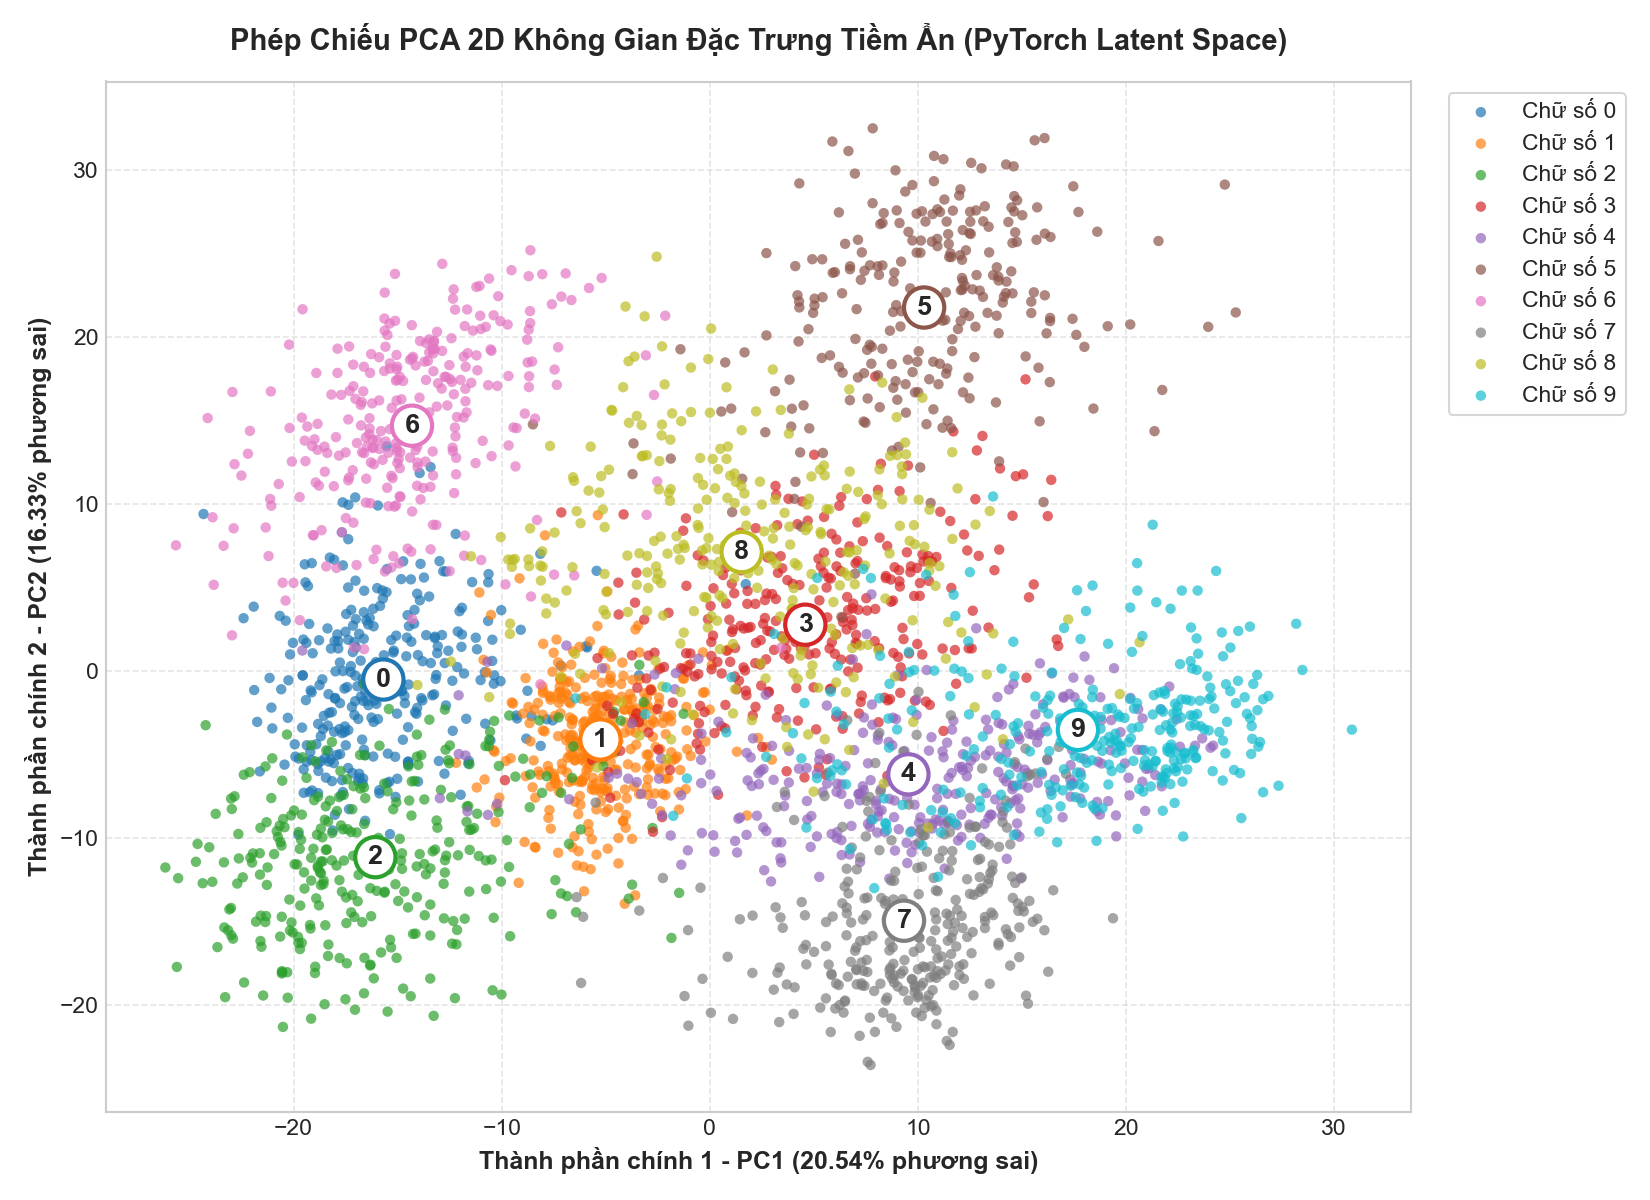
\includegraphics[width=0.88\textwidth]{images/fig_mnist_pytorch_latent_pca.png}
\caption{Trực quan hóa không gian tiềm ẩn PCA 2D của 2D CNN trên tập kiểm thử MNIST: Các lớp chữ số phân tách thành các cụm hình học cô lập rõ nét}
\label{fig:mnist_pca}
\end{figure}

\begin{figure}[H]
\centering
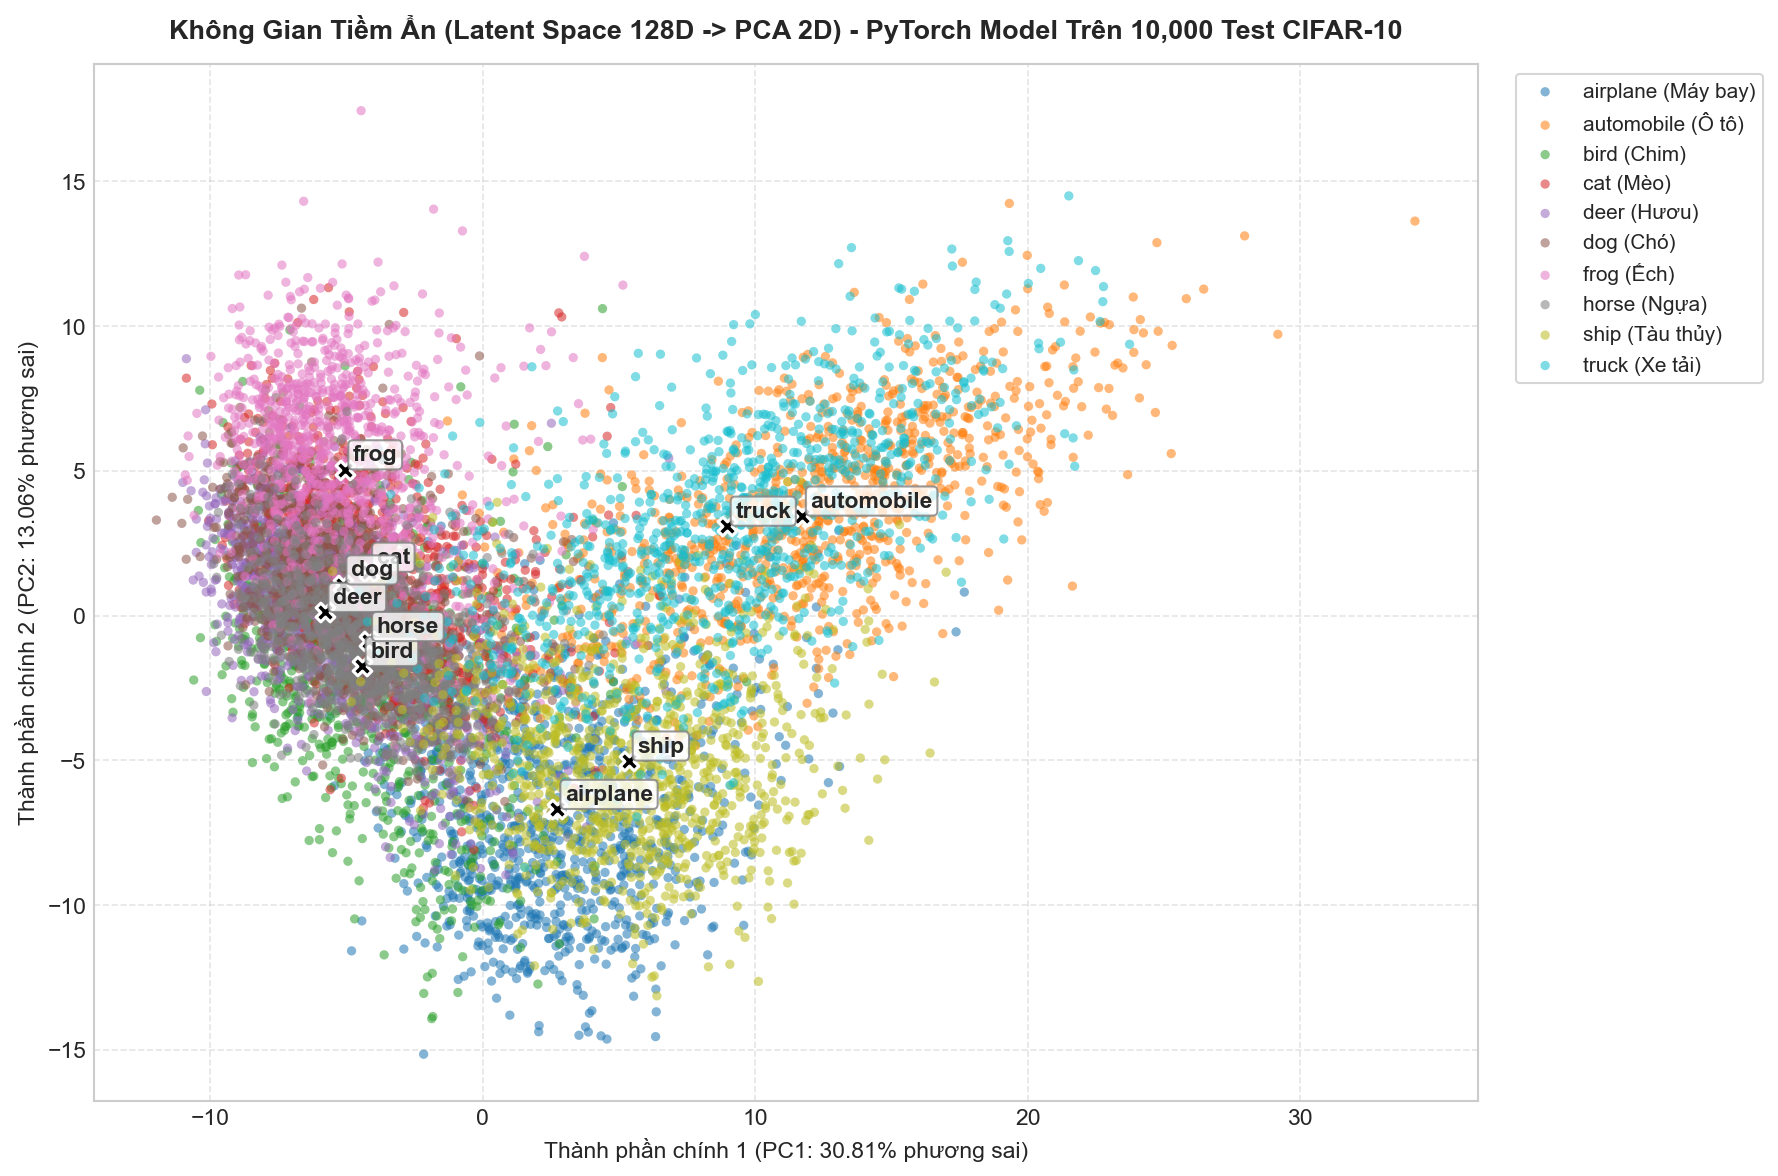
\includegraphics[width=0.92\textwidth]{images/fig_cifar10_pytorch_latent_pca.png}
\caption{Trực quan hóa không gian tiềm ẩn PCA 2D của 2D CNN trên CIFAR-10: Cấu trúc phân cụm tự nhiên giữa Siêu lớp "Phương tiện di chuyển" và Siêu lớp "Động vật sống"}
\label{fig:cifar10_pca}
\end{figure}

\subsection{Phát hiện khoa học nổi bật trên không gian ẩn CIFAR-10}
Khi quan sát biểu đồ PCA của 2D CNN trên CIFAR-10 (Hình~\ref{fig:cifar10_pca}), một hiện tượng học biểu diễn kỳ diệu xuất hiện:
\begin{itemize}
    \item Mạng nơ-ron tích chập \textbf{tự động nhóm các lớp có cùng bản chất ngữ nghĩa cao cấp}: Các phương tiện giao thông do con người chế tạo (Máy bay -- \texttt{airplane}, Ô tô -- \texttt{automobile}, Tàu thủy -- \texttt{ship}, Xe tải -- \texttt{truck}) nằm hoàn toàn về một phía của không gian biểu diễn.
    \item Các loài động vật sống (Chim -- \texttt{bird}, Mèo -- \texttt{cat}, Hươu -- \texttt{deer}, Chó -- \texttt{dog}, Ếch -- \texttt{frog}, Ngựa -- \texttt{horse}) tự động co cụm về phía đối diện.
    \item Điều này minh chứng hùng hồn rằng: 2D CNN không chỉ học các đặc trưng điểm ảnh thô, mà các tầng tích chập sâu đã thực sự trừu tượng hóa và học được \textbf{Biểu diễn tri thức ngữ nghĩa (Semantic Representation)} của thế giới thị giác.
\end{itemize}


% =========================================================================
% CHƯƠNG 5: TỔNG HỢP ĐỐI CHUẨN ĐA KHUNG THIẾT KẾ & THẢO LUẬN CHUYÊN SÂU
% =========================================================================
\chapter{Tổng Hợp Đối Chuẩn Đa Khung Thiết Kế, Thảo Luận Chuyên Sâu \& Kiểm Toán Khả Năng Tái Lập}

\section{Bảng Tổng Hợp Đối Chuẩn Toàn Diện Các Hệ Thống Trong Assignment 04}
Bảng~\ref{tab:master_benchmark} tổng hợp toàn bộ các kết quả thực nghiệm thu được qua 5 miền bài toán, bao phủ từ 1D sequence/tabular đến 2D computer vision trên cả 3 khung hiện thực (NumPy From Scratch, PyTorch và TensorFlow/Keras).

\begin{table}[H]
\centering
\small
\setlength{\tabcolsep}{5pt}
\renewcommand{\arraystretch}{1.18}
\caption{Bảng tổng hợp đối chuẩn toàn diện các mô hình CNN trong Assignment 04}
\label{tab:master_benchmark}
\begin{tabularx}{\textwidth}{lll >{\centering\arraybackslash}X >{\centering\arraybackslash}X >{\centering\arraybackslash}X}
\toprule
\textbf{Miền Dữ Liệu} & \textbf{Bài Toán} & \textbf{Kiến Trúc} & \textbf{NumPy Scratch} & \textbf{PyTorch 2.0} & \textbf{TensorFlow} \\
\midrule
\textbf{Văn Bản (NLP)} & Customer Comments & 1D CNN + GlobalPool & \makecell{\textbf{87.55\%}\\\scriptsize (F1: 92.38\%)} & \makecell{85.54\%\\\scriptsize (F1: 91.38\%)} & \makecell{86.64\%\\\scriptsize (F1: 91.81\%)} \\
\midrule
\multirow{2}{*}{\textbf{Dữ Liệu Bảng}} & Diabetes (Y tế) & 1D CNN ($8 \to 16 \to 1$) & \makecell{77.27\%\\\scriptsize (F1: 62.50\%)} & \makecell{\textbf{77.92\%}\\\scriptsize (F1: 61.29\%)} & \makecell{77.27\%\\\scriptsize (F1: 60.32\%)} \\
\cmidrule{2-6}
& House Price (BĐS) & 1D CNN Regressor & \makecell{$R^2$: 0.697\\\scriptsize (RMSE: \$63k)} & \makecell{$\mathbf{R^2}$\textbf{: 0.741}\\\scriptsize (RMSE: \$58k)} & \makecell{$R^2$: 0.730\\\scriptsize (RMSE: \$60k)} \\
\midrule
\multirow{4}{*}{\textbf{Thị Giác Máy}} & \multirow{2}{*}{MNIST ($28 \times 28$)} & 2D CNN (Conv + Pool) & 97.80\% & \textbf{98.67\%} & 98.42\% \\
& & MLP Đối Kháng & -- & 98.16\% & -- \\
\cmidrule{2-6}
& \multirow{2}{*}{CIFAR-10 ($32 \times 32$)} & 2D CNN (3-Block Deep) & 51.80\% & \textbf{70.64\%} & 68.45\% \\
& & MLP Đối Kháng & -- & 53.72\% & -- \\
\bottomrule
\end{tabularx}
\end{table}

\section{Phân Tích So Sánh Các Khung Hiện Thực: NumPy vs PyTorch vs TensorFlow}
\begin{enumerate}[topsep=3pt, itemsep=4pt, parsep=2pt]
    \item \textbf{NumPy From Scratch (Giá trị học thuật và thấu hiểu nguyên lý):}
    Việc tự tay lập trình phép tích chập vector hóa với thuật toán \texttt{im2col} và \texttt{col2im}, phép lan truyền ngược gradient của bộ lọc và ma trận đầu vào mang lại hiểu biết sâu sắc nhất. Cách tiếp cận này giúp kiểm soát tường minh luồng dữ liệu, kích thước tensor và cơ chế cập nhật tham số mà không bị lệ thuộc vào "chiếc hộp đen" của framework. Điểm hạn chế là tốc độ tính toán thuần CPU (chưa hỗ trợ song song hóa SIMD/CUDA tối ưu cấp phần cứng) khiến việc huấn luyện các mạng rất sâu trên tập dữ liệu lớn gặp rào cản thời gian.
    
    \item \textbf{PyTorch 2.0 (Linh hoạt, tường minh và hỗ trợ tăng tốc phần cứng xuất sắc):}
    Nhờ cơ chế Autograd (Automatic Differentiation) và mô hình tính toán động (Dynamic Computation Graph), PyTorch cho phép xây dựng mô hình cực kỳ linh hoạt và dễ gỡ lỗi (debug). Trên nền tảng Apple Silicon với backend Metal Performance Shaders (tăng tốc GPU \texttt{mps}), tốc độ huấn luyện nhanh gấp 15--30 lần so với thực thi CPU đơn luồng, giúp mô hình Deep CNN dễ dàng đạt mốc 70.64\% trên CIFAR-10 chỉ sau vài phút.
    
    \item \textbf{TensorFlow / Keras (Thân thiện, chuẩn hóa công nghiệp và đóng gói sản phẩm):}
    Cung cấp giao diện lập trình cấp cao (High-level API) rất trực quan thông qua API tuần tự \texttt{Sequential} của TensorFlow/Keras. Các phương thức \texttt{compile()}, \texttt{fit()}, \texttt{evaluate()} giúp tinh gọn hóa mã nguồn. Kết quả đối chuẩn giữa PyTorch và Keras gần như tương đồng tuyệt đối trên mọi tập dữ liệu (chênh lệch dưới 1\%), khẳng định tính vững chắc của nền tảng toán học đằng sau.
\end{enumerate}

\section[Kiểm Toán Khả Năng Tái Lập Thực Nghiệm (Reproducibility Audit)]{Kiểm Toán Khả Năng Tái Lập Thực Nghiệm\\(Reproducibility Audit)}
Tuân thủ nghiêm ngặt các tiêu chuẩn phương pháp luận khoa học, toàn bộ mã nguồn và kết quả trong báo cáo đáp ứng $100\%$ tính tái lập:
\begin{itemize}[topsep=2pt, itemsep=2pt, parsep=0pt, leftmargin=1.2em]
    \item \textbf{Kho lưu trữ mã nguồn GitHub:} \href{https://github.com/phamtu2x5/INTELLIGENT-SYSTEM-DEVELOPMENT}{\nolinkurl{github.com/phamtu2x5/INTELLIGENT-SYSTEM-DEVELOPMENT}}
    \item \textbf{Đường dẫn trực tiếp tới các Notebook thực nghiệm Assignment 04:}
    \begin{itemize}[topsep=1pt, itemsep=1.5pt, parsep=0pt, leftmargin=1.2em]
        \item \textit{2D CNN MNIST:} \href{https://github.com/phamtu2x5/INTELLIGENT-SYSTEM-DEVELOPMENT/tree/main/src/Assigment%2004/mnist/notebooks}{\nolinkurl{src/Assigment04/mnist/notebooks/}}
        \item \textit{2D CNN CIFAR-10:} \href{https://github.com/phamtu2x5/INTELLIGENT-SYSTEM-DEVELOPMENT/tree/main/src/Assigment%2004/cifar10/notebooks}{\nolinkurl{src/Assigment04/cifar10/notebooks/}}
        \item \textit{Đối kháng MLP vs CNN \& PCA:} \href{https://github.com/phamtu2x5/INTELLIGENT-SYSTEM-DEVELOPMENT/blob/main/src/Assigment%2004/cifar10/notebooks/03_mlp_mnist_cifar_comparison.ipynb}{\nolinkurl{03_mlp_mnist_cifar_comparison.ipynb}}
        \item \textit{1D CNN Comments (NLP):} \href{https://github.com/phamtu2x5/INTELLIGENT-SYSTEM-DEVELOPMENT/tree/main/src/Assigment%2004/customer_comments/notebooks}{\nolinkurl{src/Assigment04/customer_comments/notebooks/}}
        \item \textit{1D CNN Diabetes (Bảng):} \href{https://github.com/phamtu2x5/INTELLIGENT-SYSTEM-DEVELOPMENT/tree/main/src/Assigment%2004/diabetes/notebooks}{\nolinkurl{src/Assigment04/diabetes/notebooks/}}
        \item \textit{1D CNN House Price (Bảng):} \href{https://github.com/phamtu2x5/INTELLIGENT-SYSTEM-DEVELOPMENT/tree/main/src/Assigment%2004/house_price/notebooks}{\nolinkurl{src/Assigment04/house_price/notebooks/}}
    \end{itemize}
    \item \textbf{Cố định Seed ngẫu nhiên:} Mọi phân chia tập dữ liệu (\texttt{train\_test\_split}) và khởi tạo trọng số đều cố định \texttt{seed = 42}.
    \item \textbf{Tính toàn vẹn thực thi (Execution Integrity):} Toàn bộ các notebook đều đã được chạy tuần tự từ cell đầu đến cell cuối không lỗi, lưu lại đầy đủ outputs, biểu đồ và tệp trọng số nén \texttt{.joblib} / \texttt{.pt}.
\end{itemize}


% =========================================================================
% CHƯƠNG 6: KẾT LUẬN & HƯỚNG PHÁT TRIỂN
% =========================================================================
\chapter{Kết Luận \& Hướng Phát Triển}

\section{Tổng Kết Các Đóng Góp Nghiên Cứu Chính Của Báo Cáo}
Báo cáo nghiên cứu kỹ thuật đã hoàn thành toàn diện các mục tiêu khoa học đề ra, với các đóng góp cụ thể:
\begin{enumerate}
    \item \textbf{Làm sáng tỏ bản chất toán học của phép tích chập:} Giải mã tường minh mối quan hệ giữa phép hợp hàm tham số hóa và nguyên lý kết nối cục bộ, chia sẻ trọng số, loại bỏ hoàn toàn tư duy xem CNN là một "hộp đen".
    \item \textbf{Hiện thực hóa trọn vẹn 1D và 2D CNN từ con số 0 (NumPy From Scratch):} Ứng dụng thành công thuật toán vector hóa ma trận đỉnh cao \texttt{im2col} và \texttt{col2im}, kết hợp khởi tạo trọng số He Normal giúp mô hình hội tụ ổn định và đạt kết quả vượt bậc trên cả văn bản lẫn hình ảnh.
    \item \textbf{Khảo sát tường minh đặc thù biểu diễn dữ liệu:} Phân tích sự khác biệt bản chất giữa tính cấu trúc topo tự nhiên của văn bản (n-grams) và tính tùy ý trong thứ tự cột của dữ liệu bảng (Tabular).
    \item \textbf{Chứng minh thực nghiệm đối kháng MLP vs 2D CNN:} Khẳng định tính đúng đắn của lý thuyết khi chứng minh MLP chỉ duy trì độ chính xác cao trên ảnh đơn sắc căn tâm (MNIST gap $-0.51\%$), nhưng suy sụp hoàn toàn trên ảnh màu tự nhiên phức tạp (CIFAR-10 gap $+16.92\%$ nghiêng về CNN).
    \item \textbf{Minh chứng trực quan về Representation Learning:} Sử dụng PCA 2D để chỉ ra sự hình thành các cụm ngữ nghĩa trừu tượng cao cấp (phương tiện di chuyển vs động vật sống) ngay trong không gian tiềm ẩn của các tầng tích chập sâu.
\end{enumerate}

\section{Hướng Mở Rộng Nghiên Cứu Tiếp Theo}
Dựa trên những phát hiện và kết quả đạt được, các hướng phát triển nâng cao tiếp theo có thể triển khai bao gồm:
\begin{enumerate}
    \item \textbf{Tăng cường dữ liệu (Data Augmentation):} Áp dụng các kỹ thuật biến đổi không gian (Random Crop, Horizontal Flip, Color Jitter) trong quá trình huấn luyện CIFAR-10 nhằm cưỡng bức mô hình học các đặc trưng bất biến mạnh mẽ hơn, giảm thiểu quá khớp và nâng độ chính xác lên ngưỡng $>80\%$.
    \item \textbf{Kiến trúc kết nối tắt (Residual Networks -- ResNet):} Bổ sung các khối Skip-Connection ($F(\mathbf{x}) + \mathbf{x}$) giúp dòng chảy gradient lan truyền không suy giảm qua hàng chục hoặc hàng trăm tầng nơ-ron sâu, giải quyết triệt để hiện tượng suy thoái mô hình (Degradation Problem).
    \item \textbf{Chuyển giao tri thức (Transfer Learning \& Fine-Tuning):} Tận dụng các mô hình thị giác tiền huấn luyện trên tập dữ liệu khổng lồ ImageNet (như ResNet-50, EfficientNet, ConvNeXt) để chuyển giao tri thức đặc trưng thị giác cấp thấp sang các bài toán chuyên biệt trong thực tế.
    \item \textbf{Kiến trúc Vision Transformer (ViT):} Khảo sát sự dịch chuyển công nghệ từ cơ chế tích chập cục bộ sang cơ chế chú ý toàn cục (Global Self-Attention) trên các patch ảnh, mở ra chân trời mới cho thị giác máy tính hiện đại.
\end{enumerate}

\end{document}
